\chapter{Cross-tissue comparison of chromatin accessibility, gene expression signature and immunophenotypes in PsA}
\chaptermark{Cross-tissue comparison analysis in PsA}
\label{ch:Results3}


%%%%%%%%%%%%%%%%%%%%%%%%%%%%%%%%%%%%%%%%%%%%%%%%%%

\section{Introduction}

\subsection{The relevance of cell type and tissue specificity in the study of PsA}

Consideration of cell and type specificity in the study of complex diseases is fundamental for the understanding of the disease pathophysiology. As previously reviewed (\ref{ch:Intro}), the dysregulated immune response in PsA is the results of the interaction between cellular components of the innate and adaptive immune response. Consequently, the molecular characterisation of the different immune cell types is pivotal not only for the understanding of the immune response but also to define disease state, comprehend the impact of genetic variants increasing disease risk and identify drugs with optimal efficacy and specificity.

PsA is considered a systemic disease where studies in PBMCs have demonstrated changes in cell type composition and cytokine production when compared to healthy individuals. For example, increased frequencies of circulating IL-17$^+$ and IL-22$^+$ CD4$^+$ T cells have been reported in PB from PsA patients compared to control individuals \parencite{Benham2013}. Moreover, reduced percentage of pDCs and NK in PB have also been observed in PB from PsA compared to controls \parencite{Jongbloed2006, Spadaro2004}. In terms of cytokine production, stimulated PBMCs from PsA patients released greater levels of IL-17 and IL-22 than the healthy control counterparts \parencite{Benham2013}. 

Nevertheless, PsA is characterised by involvement of the joints, where repeated local inflammatory response leads eventually to joint destruction. Oligoarticular PsA (involving four or fewer joints) is commonly managed by joint aspiration followed by intra-articular steroid injection to relieve pain, facilitating the sample collection for research purposes \parencite{Kavanaugh2006}. The importance of studying the synovium in PsA have been highlighted by differences in cell composition and cytokine production, amongst others, between PB and SF in PsA patients. For example, expansion mCD8$^+$ but not mCD4$^+$ T cells was observed in SF when compared to PB in PsA paired samples \parencite{Ross2000}. Additionally, elevated proportion of T cells expressing the cytokine receptors CCR6$^+$ and IL-23R$^+$ were found in SF compared to PB in patients \parencite{Benham2013}. Moreover, the elevated TNF-$\alpha$, IL-1, IL-6 and IL-18 production in PsA SF was comparable to RA \parencite{Kujik2006}. 


\subsection{Bulk transcriptomic studies in PsA and their limitations}

Genome-wide transcriptomic studies in PsA have been mainly focused in characterising gene expression in bulk PBMCs and SFMCs samples. Several studies have been conducted to better understand gene expression differences in blood between PsA and controls and also specific differences between PB and SF from the same PsA patients or differences with other arthritic diseases \parencite{Stoeckman2006, Batiwalla2005, Gu2002, Dolcino2015}. Amongst the most comprehensives of these studies, that conducted by Dolcino and colleagues revealed genes from the Th-17 axis and type-I IFN signalling to be differentially expressed between PsA and healthy controls in synovial membranes. Moreover, the overlap of genes that were differentially expressed between patients and controls in each of the compartments, highlighted differences and commonalities in the systemic and synovial immune response in PsA. %Other studies have also focused in the understanding the transcriptional changes in PBMCs from PsA patients following MTX and TNFi therapies \parencite{Cuchacovich2014}. 
Cytokines production measurements have also been conducted in serum and SF, revealing increased levels of TNF-$\alpha$, for example, in both tissues when compared to controls and osteoarthritis patienst, respectively \parencite{Ritchlin1998,Li2017}. 

Studies using mixed cell populations can be influenced by the relative proportion of the different cell populations within the sample \parencite{Whitney2003}. For instance, the importance of considering cell types to understand the impact of genetic variants in transcriptional regulation has been explored in a number of immune cells \parencite{Fairfax2012, Fairfax2014, Raj2014, Peters2016, Kasela2017}. These studies have highlighted the regulatory role of some genetic variants only in particular cell types and conditions, previously masked when considering mixed population of cells such as PBMCs. In this respect, expression analysis for a limited number of genes have been performed in specific cell type populations such as stimulated macrophages and Th-17 \textit{in vitro} differentiated cells from na\"{i}ve CD4$^+$ isolated from PB and SF of PsA patients \parencite{Antoniv2006, Leipe2010}. The importance of investigating the transcriptional profile of patients' isolated discrete cell populations have yielded interesting findings in monocytes and Th-17 cells in AS, intestinal epithelial cells in CD and fibroblast-like synoviocytes in RA \parencite{Al-Mossawi2017,Smith2008, Howell2018, Ai2016}. Overall, achieving a detailed and precise understanding of complex diseases requires the study of sorted cell populations and when possible isolated from the affected tissue.  


\subsection{Transcriptomics and proteomics at the single cell resolution}

In addition to the study of specific cell types, evidence for heterogeneity in the transcriptome within cells from the same population has accelerated the development of strategies providing single cell resolution. The establishment of scRNA-seq and mass-cytometry techniques represent an unbiased way to characterise and identify cell subpopulations within the samples, avoiding the pre-selection of particular cell types and thus providing a global overview of cell composition and interactions in the tissue of interest. 

A wide range of approaches to study single-cell transcriptomics have been developed in the last few years, including Drop-seq, SmartSeq2 and 10X Chromium amongst the most widely used \parencite{Picelli2014,Ziegenhain2017}. 10X Chromium technology is based on microfluidics where cells in suspension get directly encapsulated into nanoL droplets that incorporate cell and transcript barcode identifiers (see \ref{ch:Mat}). As a result, 10X Chromium technology does not require pre-sorting of single-cells into plates and enables higher throughput than other with less manipulation and variability than other scRNA-seq methods such as SmartSeq2 \parencite{Baran-Gale2017}.
 
Mass cytometry represents the next generation of fluorescence based flow-cytometry analysis to interrogate expression of cell surface and intracellular molecules. Mass cytometry is a hybrid technique between mass spectrometry and flow cytometry, where the Abs recognising the molecular markers have been labelled with stable isotopes instead of fluorophores \parencite{Bandura2009}. The use of isotopes enables incorporating up to fourty-five Abs to profile cellular populations and assess molecular functions. 



\subsection{The challenges of using a multi-omics approach in the study of complex diseases}

The interaction between genetics and the environment can shape the cellular epigenetic landscape and eventually result in the development of complex diseases. This dynamism of the epigenome entails cell and context specific features which reinforce the importance of studying purified cell types instead of mixed populations. As previously mentioned, the epigenomic landscape has a pivotal role in understanding disease state and also contextualizing the role of putative genetic risk variants in the study of complex diseases. In this context, the implementation of multi-omics approaches in the study of complex diseases has enabled to better understand the relationship between the regulatory landscape, gene expression and protein translation in cell populations of interest. 

As previously highlighted in Chapter \ref{ch:Results2}, the methodological advances in the epigenetics field have allowed to map the regulatory landscape from clinical samples. This approach has facilitated the characterisation of the closest regulatory landscape to disease conditions using cell populations directly isolated from patients, instead of cultured cell lines or primary cells with additional stimulus, and the integration with the transcriptional profiles from paired samples. Incorporation of scRNA-seq and mass cytometry in addition to bulk RNA-seq and flow cytometry have led to a more detailed understanding of the immune system, accounting for the variability at the single-cell level in gene expression and protein translation \parencite{Jaitin2014, Villani2017,Bengsch2018}. In complex diseases such as RA, scRNA-seq has revealed heterogeneity in the synovial fibroblast population and identified a potentially pathogenic cluster highly proliferative and active in pro-inflammatory cytokine secretion \parencite{Mizoguchi2018}. Similarly, mass cytometry analysis performed in RA identified an expanded CD4$^+$ T cell population promoting B cell response \parencite{Rao2017}.



%Recent technical advances such as ATAC-seq are enabling the characterisation of the regulatory landcape in a wide range of cell types and tissues obtained from valuable clinical samples minimising the amount of material required. Profiling the chromatin accessibility in the cell populations isolated from the tissues of interest provides details about the molecular programming of cells and can also inform about the location and status of \text{cis}-regulatory elements. For example differential analysis in B cells isolated from SLE and healthy controls has revealed changes in chromatin accessibility for loci nearby genes involved in B cells activation and enrichment for TFBS potentially regulating pathogenic processes \parencite{Scharer2016}. Similarly a study in age-related macular degeneration (AMD) has identified the retina epithelium as the main tissue driving disease onset though global loss of chromatin accessibility compared to healthy tissue \parencite{Wang2018}. 


One of the most challenging aspects of using a multi-omics approach is the appropriate integration of the data in order to maximise the amount of information extracted and also the reliability of the findings. The power of this integration is increased by generating paired data for all the omics across all the individuals in the cohort, which cannot always be achieved due to sample availability and cost. Recently, Zhang and colleagues have published one of the most comprehensive available study integrating multi-omics (bulk RNA-seq, scRNA-seq and mass cytometry) in RA \parencite{Zhang2018}. This study performed isolation of the main pathophysiological cell types infiltrated into RA synovial membranes, including T cells, B cells, monocytes, and fibroblasts, and identified eighteen unique subpopulations by systematic correlation between transcriptional profiles and mass cytometry.



\subsection{Integration of fine-mapping GWAS SNPs and functional data in PsA}

As already explained in Chapters \ref{ch:Intro} and \ref{ch:Results2}, fine-mapping of the GWAS signals is required in order to reduce the putative number of causal SNPs accounting for a particular association in complex diseases. Fine-mapping using genotype level data incorporates a locus step-wise conditional analysis to identify independent secondary signals, prior to calculate PP and credible sets for each of them \parencite{Maller2012,Bunts2015}. In some cases, this enables to reduce the size of the region associated to disease and thus the number of putative causal SNPs that could be functionally relevant for the disease pathophysiology. Although fine-mapping reduces the number of putative causal SNPs from thousands to tens, additional integration of epigenetics and functional data as well as molecular assays are required to pinpoint the genetic variant and the mechanisms driving the association with disease.  

The PsA GWAS study conducted by Bowes and colleagues successfully performed fine-mapping for seventeen of the associated regions \parencite{Bowes2016}. This study provided a summary table for the overlap of SNPs from the 90\% credible set (list of SNPs explaining 90\% of the PsA GWAS association) with genomic annotations and ENCODE features (cell lines and healthy donors primary cells), to further narrow down the set of putative causal SNPs for each associations as well as the more relevant cell type where they may have an effect. Bowes \textit{et al.} further investigated the PsA-specific association identified in this study at the 5q31 region and a pilot eQTL study confirmed the most significant correlation with \textit{SLC22A5} expression for a SNP in high LD with the GWAS lead SNP.

Leveraging epigenetic data to further refine the candidate causal SNPs from fine-mapping studies could benefit from the generation of disease-specific chromatin regulatory maps in PsA affected tissue and, possibly, further integration of scRNA-seq and mass cytometry from the same individuals. Altogether, this data could represent an additional layer of information in the attempt to identify the causal variant driving GWAS associations with PsA and provide further insight into the disease pathophysiology. 

%Fine-mapping has been systematically applied to a number of immune-mediated GWAS, including T2D, IBD, AS and SLE \parencite{Maller2012,Gaulton2015,Bunt2015,Sun2016,Huang2017}. In contrast, systematic fine-mapping studies for all the sixty-three psoriasis GWAS loci have not been performed yet. In PsA, Bayesian fine-mapping has been conducted for some of the Immunochip GWAS associations, including the 5q31 PsA-specific locus  \parencite{Bowes2015}.
%
%% Maybe in the discussion
%Regardless the contribution towards dissecting causality, traditional Bayesian fine-mapping models assume only one causal SNP driving the association at each locus. As a way to partially address this limitation, these methods include a locus step-wise conditional analysis to identify independent secondary signals, prior to calculate PP and credible sets for each of them \parenicte{Maller2012,Bunts2015}. Improved methods such as stochastic Bayesian fine-mapping outperforms the step-wide Bayesian approached by avoiding the biases of the conditional analysis and considering all the possible models regarding number of putative causal SNPs to explain association of each locus \parencite{Wallace2016}
%
%The resolution of fine mapping studies could be enhanced by the integration of trans-ethnic fine-mapping meta-analysis, particularly by the inclusion of Yoruba (YRI) and Chinese Han (CHB) descendents 1000 Genomes samples with reduced LD blocks, that can shed light on the true independence of secondary signals \parencite{Bunt2015, Kichaev2015}.
%
%Recently, publicly available tools such as fGWAS and PAINTOR have leveraged cell type-specific annotation to inform the Bayesian analysis and output a further refine credible set of SNPs with functional relevance \parencite{Pickrell2014,Kichaev2015}.

%Traditional Bayesian fine-mapping models assume in the model only one causal SNP driving the association at each locus. As a way to partially address this limitation, genotype level fine-mapping incorporates a locus step-wise conditional analysis to identify independent secondary signals, prior to calculate PP and credible sets for each of them \parencite{Maller2012,Bunts2015}. A disadvantage of the methods performing fine-mapping from summary statistics data is the impossibility to perform this conditional analysis.



\section{Aims}

%In the context of technological advances in the epigenetic, transcriptomic and proteomic fields, a comprehensive multi-omic study in PsA samples to investigate discrete cell populations in circulation and at the site of inflammation has not yet been conducted. 
This chapter aims to develop a framework for the integration of a mutli-omic dataset in PsA blood and synovial immune cells. Specifically, using the chromatin accessibility landscape and the transcriptomic profile in a number of immune relevant genes in four cell populations isolated from SF and PB to improve the understanding of cell and tissue-specific differences and the relationship between chromatin accessibility and gene expression in PsA. Moreover, single-cell transcriptomic and mass cytometry will attempt to identify common and tissue-associated cell subsets contributing to pathophysiological relevant pathways in PsA and chronic inflammation. Lastly, fine-mapping of PsA GWAS loci and integration with chromatin accessibility maps of relevant immune cells from PsA samples will be performed to further narrow down the putative causal variants driving such associations. 


Specifically, the aims of this chapter are:


\begin{enumerate}
\item To identify differences in the chromatin accessibility landscape between SF and PB in CD14$^+$ monocytes, mCD4$^+$, mCD8$^+$ and NK cells isolated from PsA patients.
\item To characterise differences in the transcriptomic profiles between SF and PB for relevant immune genes in CD14$^+$ monocytes, mCD4$^+$ and mCD8$^+$ from the same PsA patients.
\item To integrate differences in chromatin accessibility and changes in genes expression from SF and PB.  
\item To further explore transcriptional differences at the single-cell level in cell types of interest and perform a basic integration with mass cytometry data.
 \item To conduct fine-mapping for a number of PsA GWAS loci using genotype data.
\item To integrate the credible set of SNPs identified by fine-mapping with cell and tissue-specific PsA chromatin accessibility maps and publicly available epigenetic and functional data to further narrow down the putative causal SNPs driving such associations.
\end{enumerate}


%Example in PsA
 %For example, a genome-wide study of the methylome in PsA PBMCs revealed a hypomethylated pattern in na\"{i}ve patients compared to those under MTX treatment \parencite{Kim1996}. 


%%%%%%%%%%%%%%%%%%%%%%%%%%%%%%%%%%%%%%%%%%%%%%%%%%
\section{Results}
%

\subsection{PsA patients cohort description and datasets}
In this study peripheral blood (PB) and SF were collected from a cohort of six PsA patients, with equal numbers of males and females (Table \ref{tab:PSA_cohort_metadata}). All the patients presented oligoarticular joint affection and had been first diagnosed with psoriasis. The cohort presented a mean of 1.5 tender or swollen affected joints (TJC66 and SJC66), which is characteristic of the oligoarticular form of disease, involving four or fewer joints. Regarding global assessment, the mean scores for the patient and physician evaluation were 3.2 and 3, respectively, in a scale of 1 to 5. These four measurements including joints and global assessment compose the PsARC disease activity scores, used by clinicians as the main indicator of response to treatment by recommendation of the National Institute for Health and Care Excellence (NICE) (Chapter \ref{ch:Intro}). 

The mean age of the cohort at the time of diagnosis was 44.3 years old and the mean disease duration 8.8 years. Interestingly, PsA1728 was diagnosed at a later age compared to the other patients in the cohort (late PsA onset clinical significance??). Moreover, C-reactive protein (CRP) levels, a further marker of inflammation, presented an average of 17.45 mg/L and was particularly higher in PsA1719 and PsA1728 compared to the other patients. At the time of sample recruitment all the PsA patients were not on active immunosupressive therapy. Post-visit, most of the patients qualified for TNAi biologic therapy xxxx.


%
\begin{landscape}
\begin{center}
\begin{longtable}[ht]{c c c c c c c c c}
%{p{.15\textheight} p{.15\textheight} p{.25\textheight} p{.25\textheight} p{.15\textheight} p{.15\textheight} p{.15\textheight}}
\caption[Description and metadata of the PsA patients cohort.]{\textbf{Description and metadata of the PsA patients cohort.}. PsARC disease activity score is composed of tender joint count 66 (TJC66) and swollen joint count 66 (SJC66), joint pain (4 point score) and self-patient and physician global assessment (5 point score). Joint pain and global assessment use a likert scale based on questionnaire answers that measure the level of agreement with each of statements included. C-reactive protein (CRP).}
\label{tab:PSA_cohort_metadata} \\
\toprule
\textbf{ Sample ID} & \textbf{Sex} & \textbf{Age at} & \textbf{Disease duration} & \textbf{Type} &\textbf{TJC66/SJC66}  & \textbf{Physician } & \textbf{Patient} & \textbf{CRP} \\
                   &               & \textbf{diagnosis} & \textbf{(months)}      &               &                      & \textbf{assessment} & \textbf{assessment}  & \textbf{(mg/L)} \\
\midrule
\midrule
PsA1718 & Female & 17 & 180 & Oligo  & 2/2 & 3 & 3 & 6 \\
PsA1719	& Male &	33 & 24	 & Oligo &	1/1 &	3 & 4 & 36.6 \\           
PsA1607 &	Male & 42 & 108 &	Oligo &	1/1	& 4 & 3 & 8 \\
PsA1728	& Female & 72	& 48 & Oligo & 2/2 & 3 & 4 & 43.2 \\
PsA1801	& Female & 53 & 168 & Oligo & 2/2 &	3 & 3 & 9.9 \\
PsA1505 & Male & 35 &	108 & Oligo & 1/1 & 2 & 2 & 1 \\	
\midrule
Average		& $-$	&	44.3 & 106 & $-$ & 1.5/1.5 & 3 & 3.2 & 17.4 \\																			
\bottomrule
\medskip
\end{longtable}
\end{center}
\end{landscape}

%\clearpage

For each of the patients, paired PB and SF data was generated from bulk or isolated cell types of interest (detailed in Table \ref{tab:PSA_datasets_per_sample} and Chapter \ref{ch:Mat}). Due to project constrains, Fast-ATAC, PCR gene expression array, scRNA-seq and mass cytometry were not generated for all six individuals in the cohort. 

\begin{table}[htbp]
%\setlength{\tabcolsep}{20pt} only to stretch the columns if you want
%\renewcommand{\arraystretch}{1.5}
\centering
\begin{tabular}{@{} c c c c c}
\toprule
\textbf{Sample ID} & \textbf{ATAC} & \textbf{RNA PCR array} & \textbf{scRNA-seq} & \textbf{Mass cytometry} \\
\midrule
\midrule
PsA1718 & Yes & No & No & Yes\\
PsA1719 & Yes & Yes & No & Yes\\
PsA1607 & Yes & Yes & Yes & Yes\\
PsA1728 & No & Yes & No & Yes\\
PsA1801 & No & No & Yes & Yes\\
PsA1605 & No & No & Yes & Yes\\
\bottomrule
\end{tabular}
\medskip %gap
\caption[Datasets generated for each sample in the PsA cohort.]{\textbf{Datasets generated for each sample in the PsA cohort.} Four types of data were generated in paired SF and PB from the same individual. The available datasets vary between individuals due to project constrains. Fast-ATAC data was generated for CD14$^+$, mCD4$^+$, mCD8$^+$ and NK cells. RNA expression by PCR array was performed only for CD14$^+$, mCD4$^+$ and mCD8$^+$ cells. scRNA-seq data was generated using 10X technology in bulk SFMCs and PBMCs.}
\label{tab:PSA_datasets_per_sample}
\end{table}
\bigskip %bigger space

\subsection{Immune cellular composition of blood and synovial fluid in the PsA cohort}
The immune cellular composition of three PsA samples (PsA1718, PsA1719 and PsA1607) was characterised in SF and PB using the ICS mass cytometry panel in Chapter \ref{ch:Mat}. For both tissues, mCD4$^+$ (between 32.1 and 55.6\%) constituted the most abundant cell type followed by mCD8$^+$ (between 16.9 and 24.9\%) and CD14$^+$ "non-classical" monocytes (between 6.9 and 21.7\%). Consistently with previous studies, a trend of increased percentage of mCD8$^+$ pDCs and cDCs was observed in SF compared to PB \parencite{Ross2000,Jongbloed2006}. This data also showed reduced percentage of SF NK cells percentage compared to PB, in line with previous studies suggesting the role of impaired non-MHC-restricted cytotoxicity in PsA \parencite{Spadaro2004}. Similarly, a tendency towards reduced proportions of B cells in SF compared to PB reinforced the lack of contribution of the humoral immune response in PsA pathophysiology. The observed differences in cell composition between SF and PB were not statistically significant for any of the twelve analysed populations likely due to the small samples size (n=3) available for the analysis. Further increase in the sample size will probably prove statistical significance for the observed differences in immune cell composition between the two tissues reproducing the results published by other studies.   

% Add the markers used to define each of the cell types and calculation of percentages based on the the total number of cells in the cluster
\begin{figure}[H]
\centering
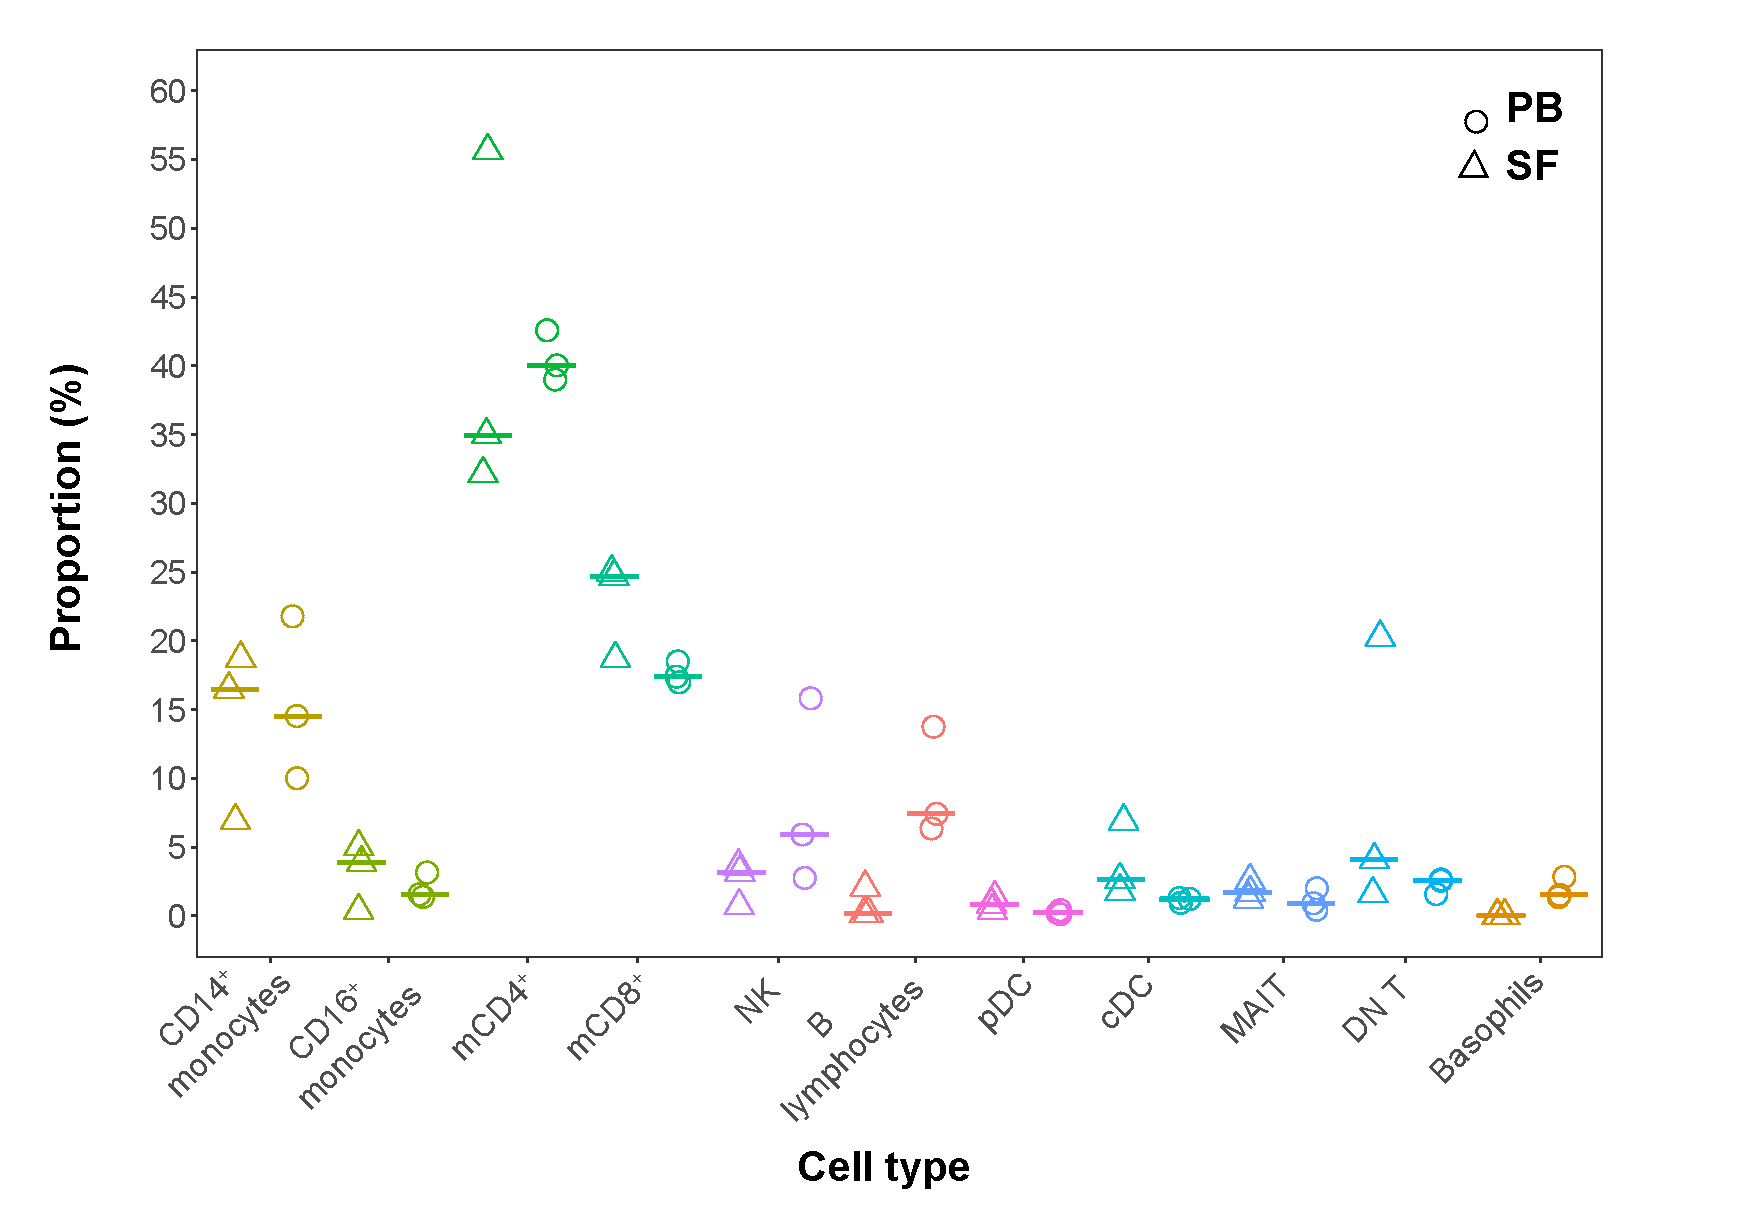
\includegraphics[width=0.7\textwidth]{./Results3/pdfs/PSA_ATAC_cohort_cell_type_composition_boxplots}
\caption[Comparative percentages of PB and SF immune cellular composition from the PsA cohort.]{\textbf{Comparative percentages of PB and SF immune cellular composition from the PsA cohort.} Percentages of each of the twelve cell types identified by mass cytometry are shown by individual and tissue for PsA1718, PsA1719 and PsA1607. Horizontal line represents the median percentage for a particular cell type in the appropriate tissue (SF or PB). Each of the cell types is displayed in a different colour. Central DC=cDC, mucosal-associated invariant T=MAIT, DN=double negative. Data analysis conducted by Dr Nicole Yager.)}
\label{figure:PsA_cell_composition}
\end{figure}



\subsection{Differential chromatin accessibility analysis in immune cells reveals differences between SF and PB}

\subsubsection{Quality control of Fast-ATAC data}
Twenty four Fast-ATAC PsA samples from four different cell types and two tissues (PB and SF) were sequenced and processes using the in-house pipeline as previously detailed in Chapter \ref{ch:Mat}. After filtering for low quality mapping, duplicates and MT reads, the median of total number of reads ranged between 46.6 and 70.2 millions (Figure \ref{figure:PsA_FAST_ATAC_QC} a). Overall, MT and duplicated reads accounted for a median of 40 to 62.2\% from the total number of unfiltered reads depending on cell type (Figure \ref{figure:PsA_FAST_ATAC_QC} b), contributing to the loss of reads in ATAC as previously detailed in Chapter \ref{ch:Results1}. %The final number of reads remaining after filtering was inversely related to the percentage of MT and duplicated reads identified. For example, mCD14$^+$ and mCD8$^+$ presented the lowest median of total number of reads after filtering concomitantly with the greatest percentage of combined MT and duplicated reads. 
%As previously mentioned, the MT DNA in ATAC-seq is one of the main sources of read loss, which is more accessible to the Tn5 transposase due to the absence of nucleosomes. Although the FAST-ATAC protocol represented an improvement, the percentage of MT reads across amongst all the samples ranged between 2.1 and 25.4\%. Similarly, despite initial optimisation of the number of PCR cycles used in the library amplification, the duplicated reads still represented between 22.9 to 55\% of the total number sequenced reads.

Regarding sample quality, TSS enrichment analysis showed differences in the levels of background noise across cell types and highlighted the variability of ATAC performance (Figure \ref{figure:PsA_FAST_ATAC_QC} c). A general trend towards greater TSS enrichment in PB samples compared to SF was observed. mCD4$^+$ and mCD8$^+$ presented the best signal-to-noise ratios, with median of 19.1 and 23.1 fold enrichment, respectively. In contrast, NK was the cell type with the lowest TSS enrichment values. Particularly, the fold enrichment for PsA1719 and PsA1607 in NK were close to the 6 fold enrichment considered by ENCODE as acceptable. Given the limited cohort size, these samples were not excluded, but it is worth noting that they could be contributing noise and thus reducing the power of the differential analysis.

 
\bigskip
\begin{figure}[H]
\centering
\begin{subfigure}[b]{0.48\textwidth}
\centering 
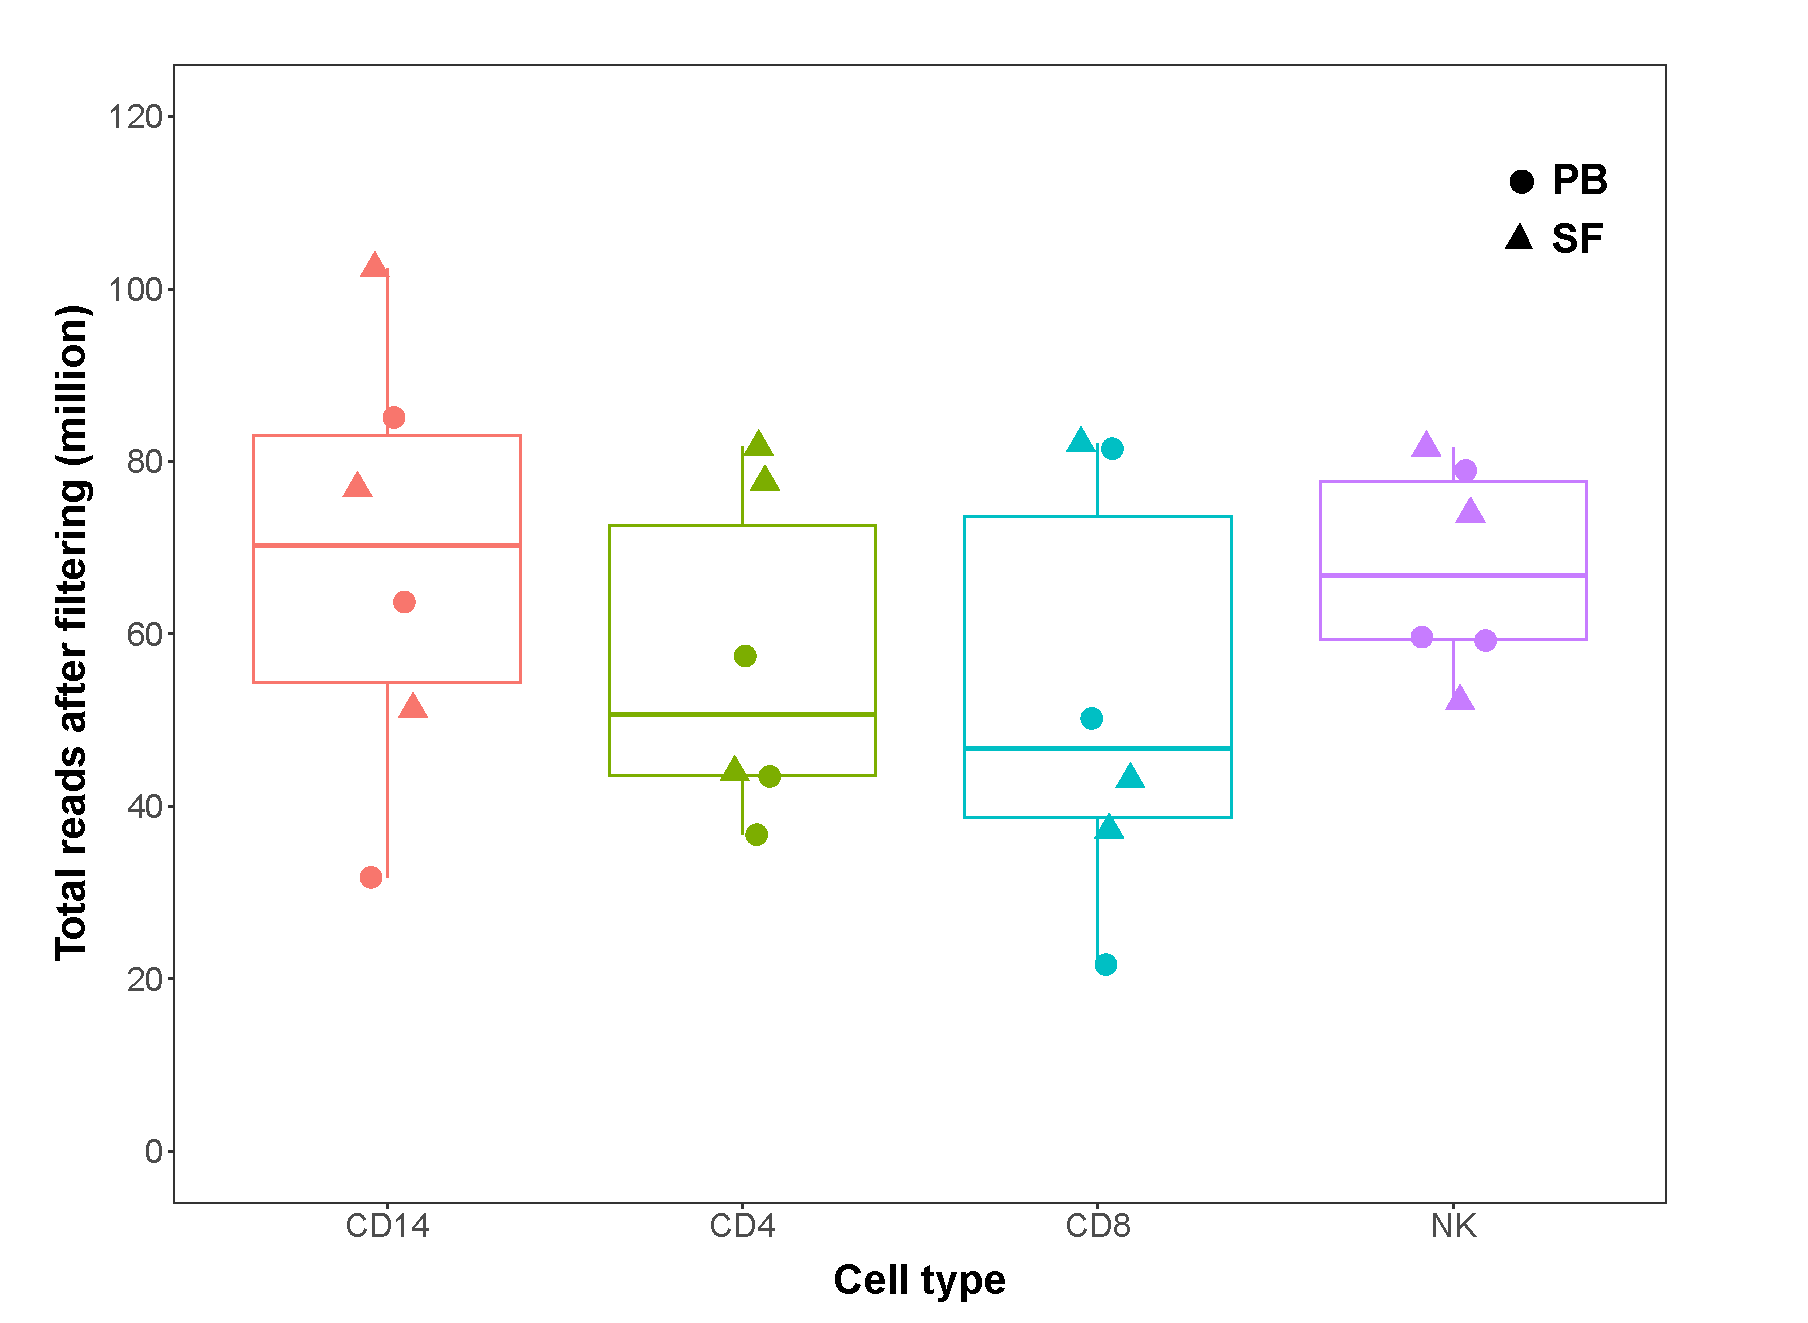
\includegraphics[width=\textwidth]{./Results3/pdfs/ATAC_PSA_total_filtered_reads_boxplot}
\caption{}
\end{subfigure}
~
\begin{subfigure}[b]{0.48\textwidth}
\centering 
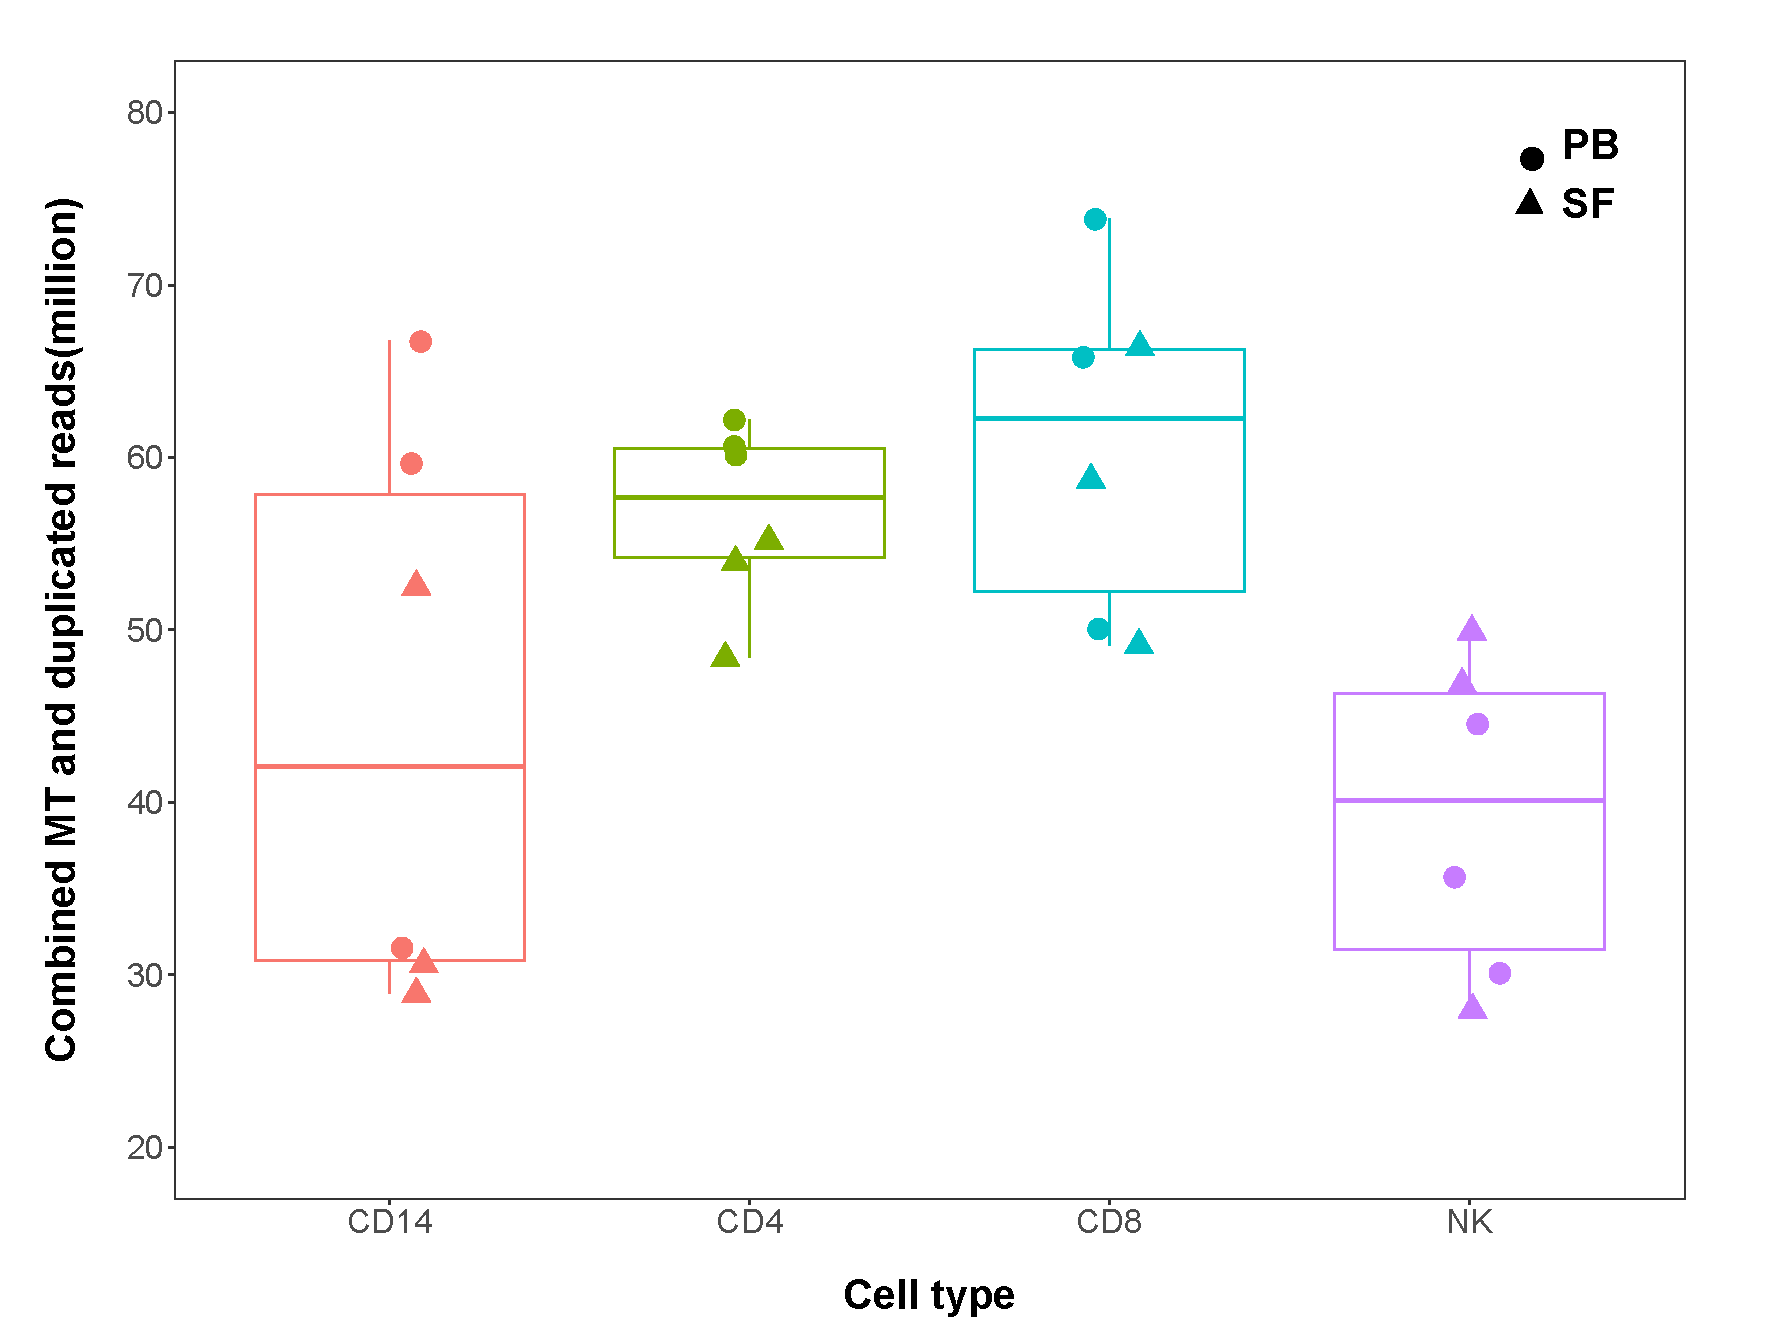
\includegraphics[width=\textwidth]{./Results3/pdfs/ATAC_PSA_pcnt_dups_and_MT_reads_boxplot}
\caption{}
\end{subfigure}
~
\begin{subfigure}[b]{0.48\textwidth} 
%the [b] prevents offset in subcaptions
\centering
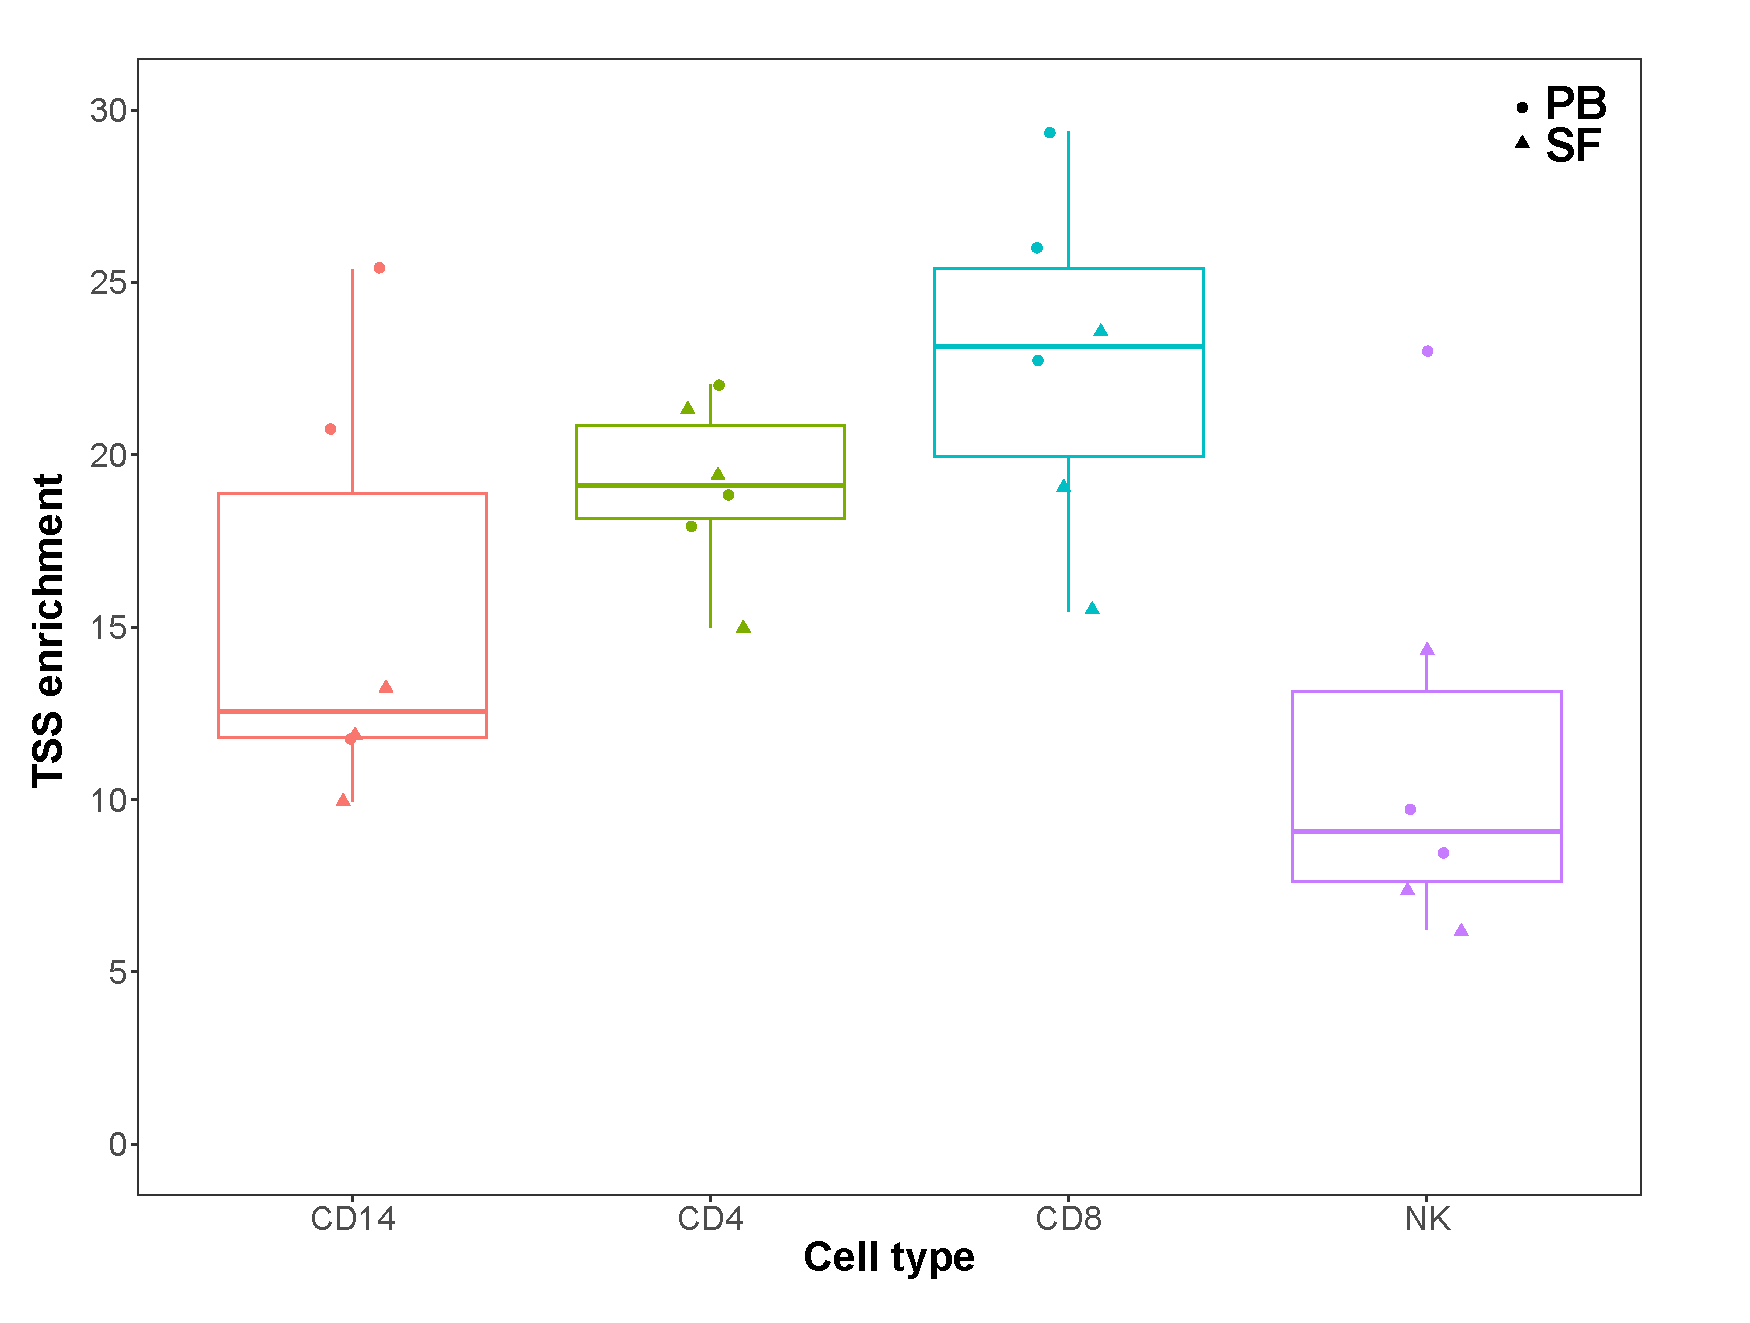
\includegraphics[width=\textwidth]{./Results3/pdfs/ATAC_PSA_all_TSS_max_per_cell_type}%
\caption{}
\end{subfigure}
\begin{subfigure}[b]{0.48\textwidth} 
%the [b] prevents offset in subcaptions
\centering
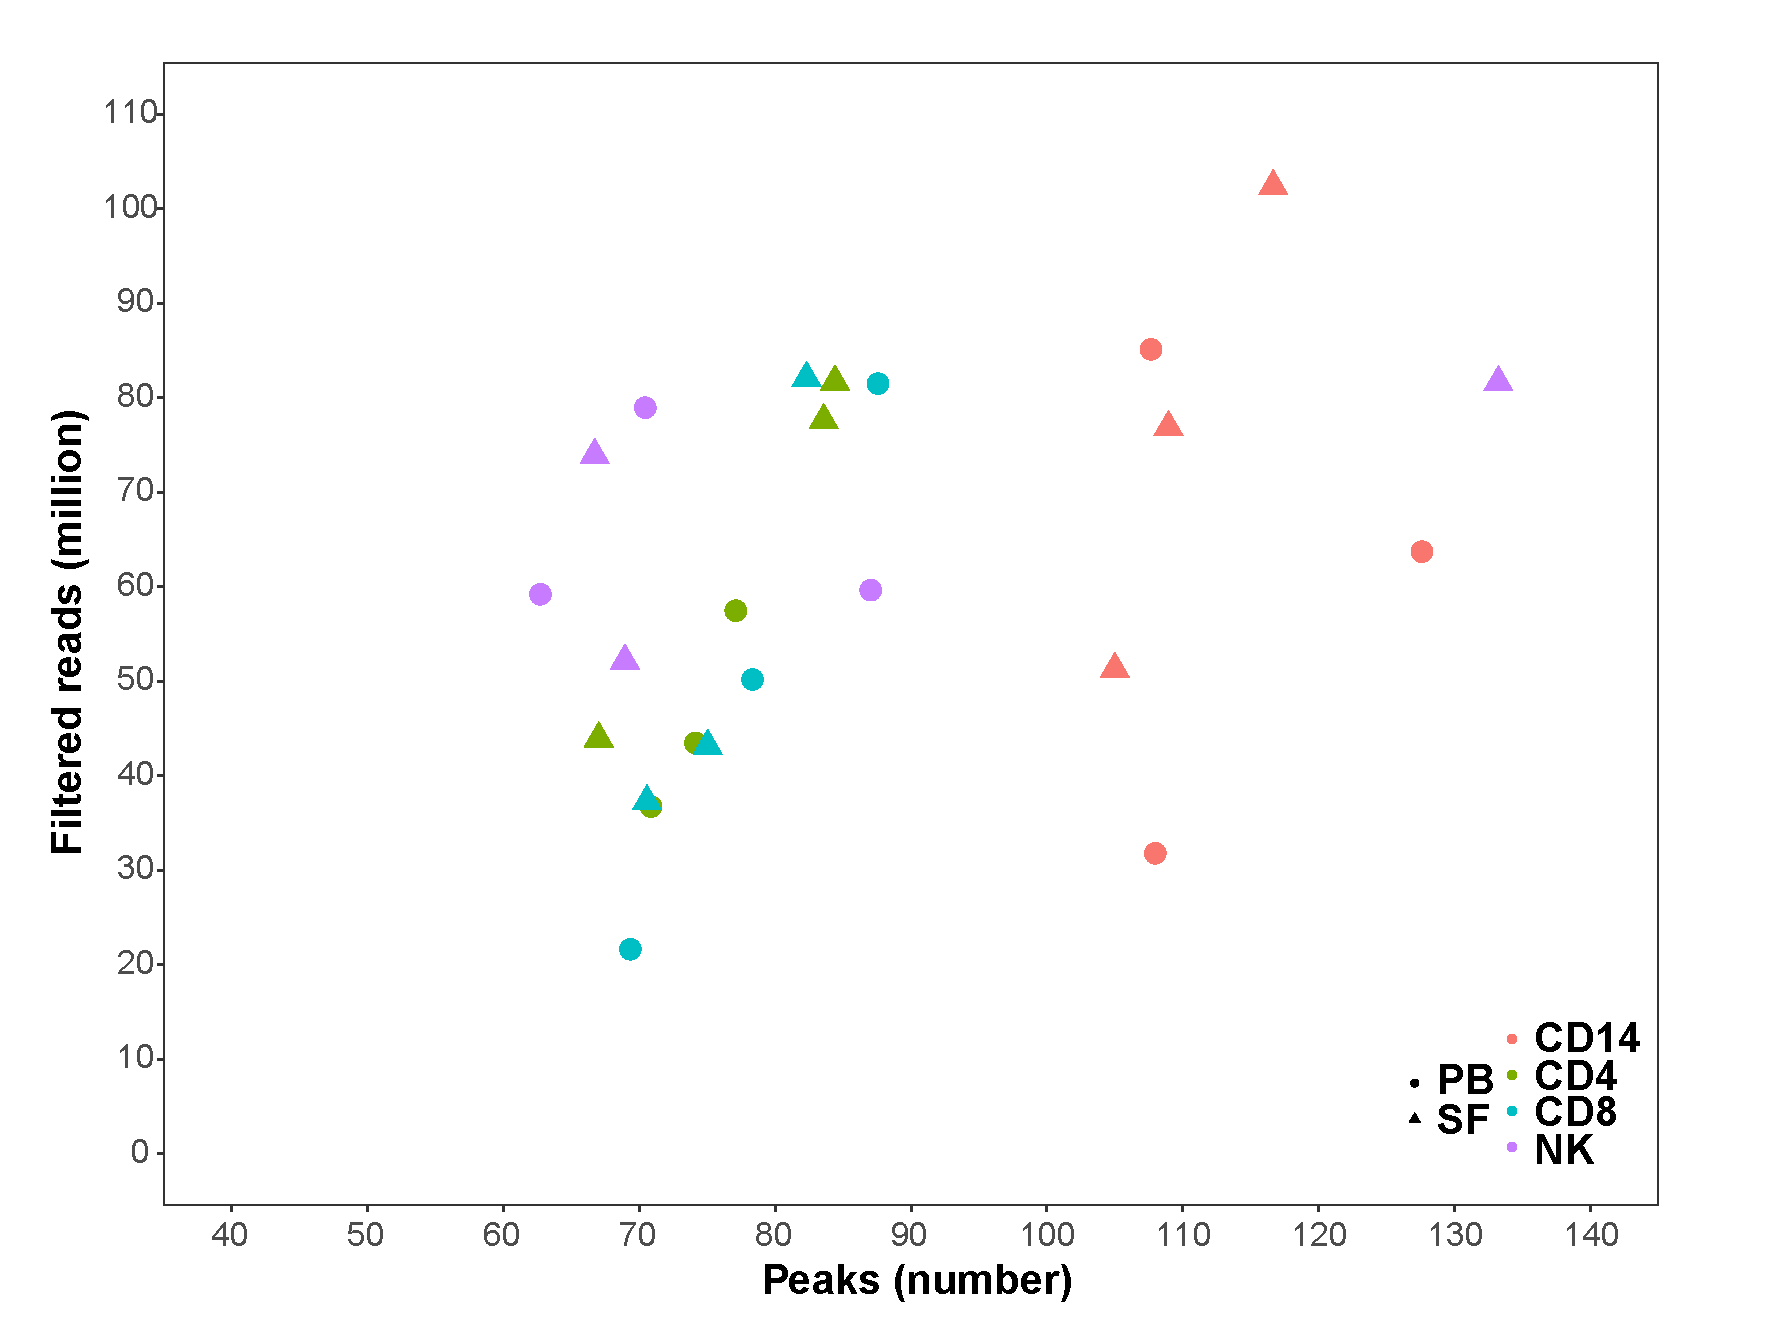
\includegraphics[width=\textwidth]{./Results3/pdfs/ATAC_PSA_all_peaks_vs_num_reads}%
\caption{}
\end{subfigure}
\caption[Quality control assessment of ATAC data generated in four immune cell types isolated from PB and SF of PsA patients samples.]{\textbf{Quality control assessment of ATAC data generated in four immune cell types isolated from PB and SF of PsA patients samples.} For each of the cell types and samples, boxplots representing a) million of reads after filtering, b) million of duplicated and MT reads combined and c) values for fold-enrichment of ATAC fragments across the Ensembl annotated TSS. In c) the dashed red line indicates the recommended Encode threshold for TSS enrichment values. d) Representation of the  number of significant peaks based on IDR optimal pval versus the total million reads after filtering for each of the samples. For each point, colour codes for cell type and shape for tissue (SF or PB).}
\label{figure:PsA_FAST_ATAC_QC}
\end{figure}


When identifying open chromatin regions by peak calling followed by pval filtering based on IDR analysis, the number of accessible regions per sample ranged approximately between 24x10$^3$ and 97x10$^3$ (Figure \ref{figure:PsA_FAST_ATAC_QC} d). The total number of called peaks passing filtering varied across cell types and was influenced by the quality sample, as previously demonstrated in Chapter \ref{ref:Results1}. Overall, appropriate number of peaks were called in all the samples and no concerning outliers were identified.
%For example, CD14$^+$ was the cell type with greatest number of called peaks (108.4$x10^3$) as well as the greater median of reads remaining after filtering when compared to the other three cell types (Figure \ref{figure:PsA_FAST_ATAC_QC} a). 
%For example, the two NK samples with the greatest TSS enrichment (PSA1718 SF and PB) showed larger number of called peaks when compared to the other NK samples with similar number of reads but lower quality measured by TSS enrichment. This observation was consistent with the correlation between sample quality and the number of identified accessible chromatin regions previously demonstrated in Chapter \ref{ch:Results1}. 


\subsubsection{Accessible chromatin reflects cell type specificity and functional relevance}
A consensus master list of accessible chromatin regions identified across all the samples and cell types (ML\_all) was built, as previously explained in Chapter \ref{ch:Mat} and Chapter \ref{ch:Results1}. PCA analysis based on the normalised counts for each region of the ML\_all showed that most of the variability (PC1 65.6\% of the variability) in the chromatin landscape correlated with cell type, leading to sample separation in four cluster (Figure \ref{figure:PsA_FAST_ATAC_PCA}). The myeloid (CD14$^+$ monocytes) and lymphoid (mCD4$^+$ and mCD8$^+$) clusters appeared as the most different between them based on the Fast-ATAC profile. Conversely,the mCD4$^+$ and mCD8$^+$ clusters were the most similar between them, altogether supporting the ability of Fast-ATAC to capture cell type chromatin accessibility features. In addition to this, modest separation between SF and PB samples was also found in the mCD4$^+$, mCD8$^+$ and NK clusters (Figure \ref{figure:PsA_FAST_ATAC_PCA}).

\begin{figure}[H]
\centering
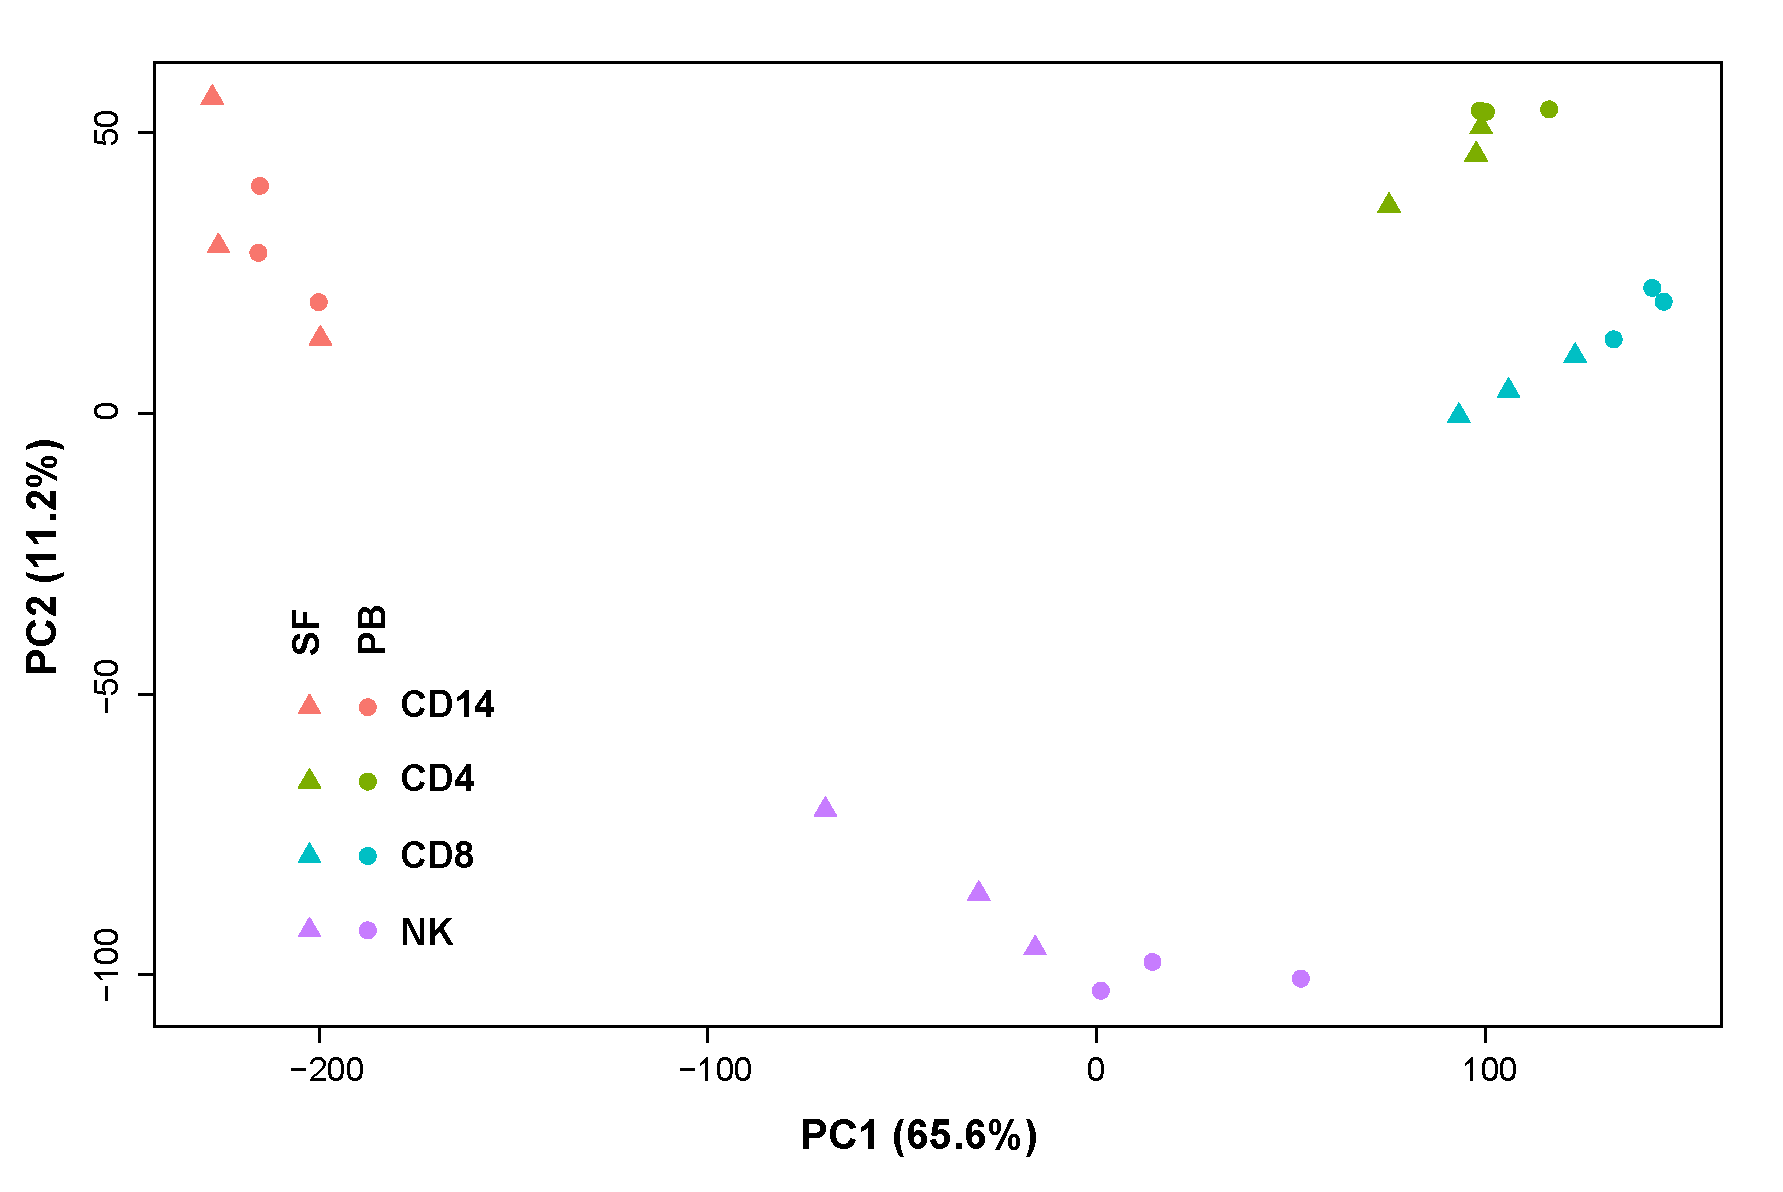
\includegraphics[width=0.6\textwidth]{./Results3/pdfs/ATAC_PSA_all_DESEq2_PCA}
\caption[PCA analysis based on the ATAC chromatin accessibility landscape in four immune cell types isolated from blood and SF.]{\textbf{PCA analysis based on the ATAC chromatin accessibility landscape in four immune cell types isolated from blood and SF.} PCA analysis was performed using the normalised counts from the combined consensus master list (ML\_all) across the four cell types (CD14$^+$ monocytes, mCD4$^+$, mCD8$^+$ and NK cells) and two tissues (SF and PB) of interest. The first two PCs (x-axis and y-axis, respectively) for the ATAC peaks included in the ML\_all are plotted. Each point represents a sample, where colour indicates cell type and shape tissue (SF and PB). The proportion of variation explained by each principal component is indicated.}
\label{figure:Core_ATAC_all_conditions_PCA}
\label{figure:PsA_FAST_ATAC_PCA}
\end{figure}



The ability to capture putative regulatory regions within the identified accessible chromatin regions was also explored. Enrichment analysis of different eQTL publicly available datasets for the regions contained in the MASTER\_ALL list was performed. Amongst the GTEx eQTL data, the largest (z-score) and most significant (-log$_10$FDR) enrichment was found for the venous blood data set (red dot), consistent with the cell types included in the study (Figure \ref{figure:PsA_FAST_ATAC_eQTL_enrichment} a). In terms of publicly available eQTLs studies in immune cells, the strongest enrichment for the MASTER\_ALL regions were found for CD14$^+$ monocytes (importantly unstimulated, LPS 2h and IFN-$\gamma$ 24h) followed by mCD8$^+$ T cells (Figure \ref{figure:PsA_FAST_ATAC_eQTL_enrichment} b). eQTLs in B cell appeared as the least enriched when compared to the other datasets, consistently with the absence of this cell type in the ATAC experiments, and reinforcing the cell specificity captured by this assay.

\bigskip
\begin{figure}[H]
\centering
\begin{subfigure}[b]{0.5\textwidth}
\centering 
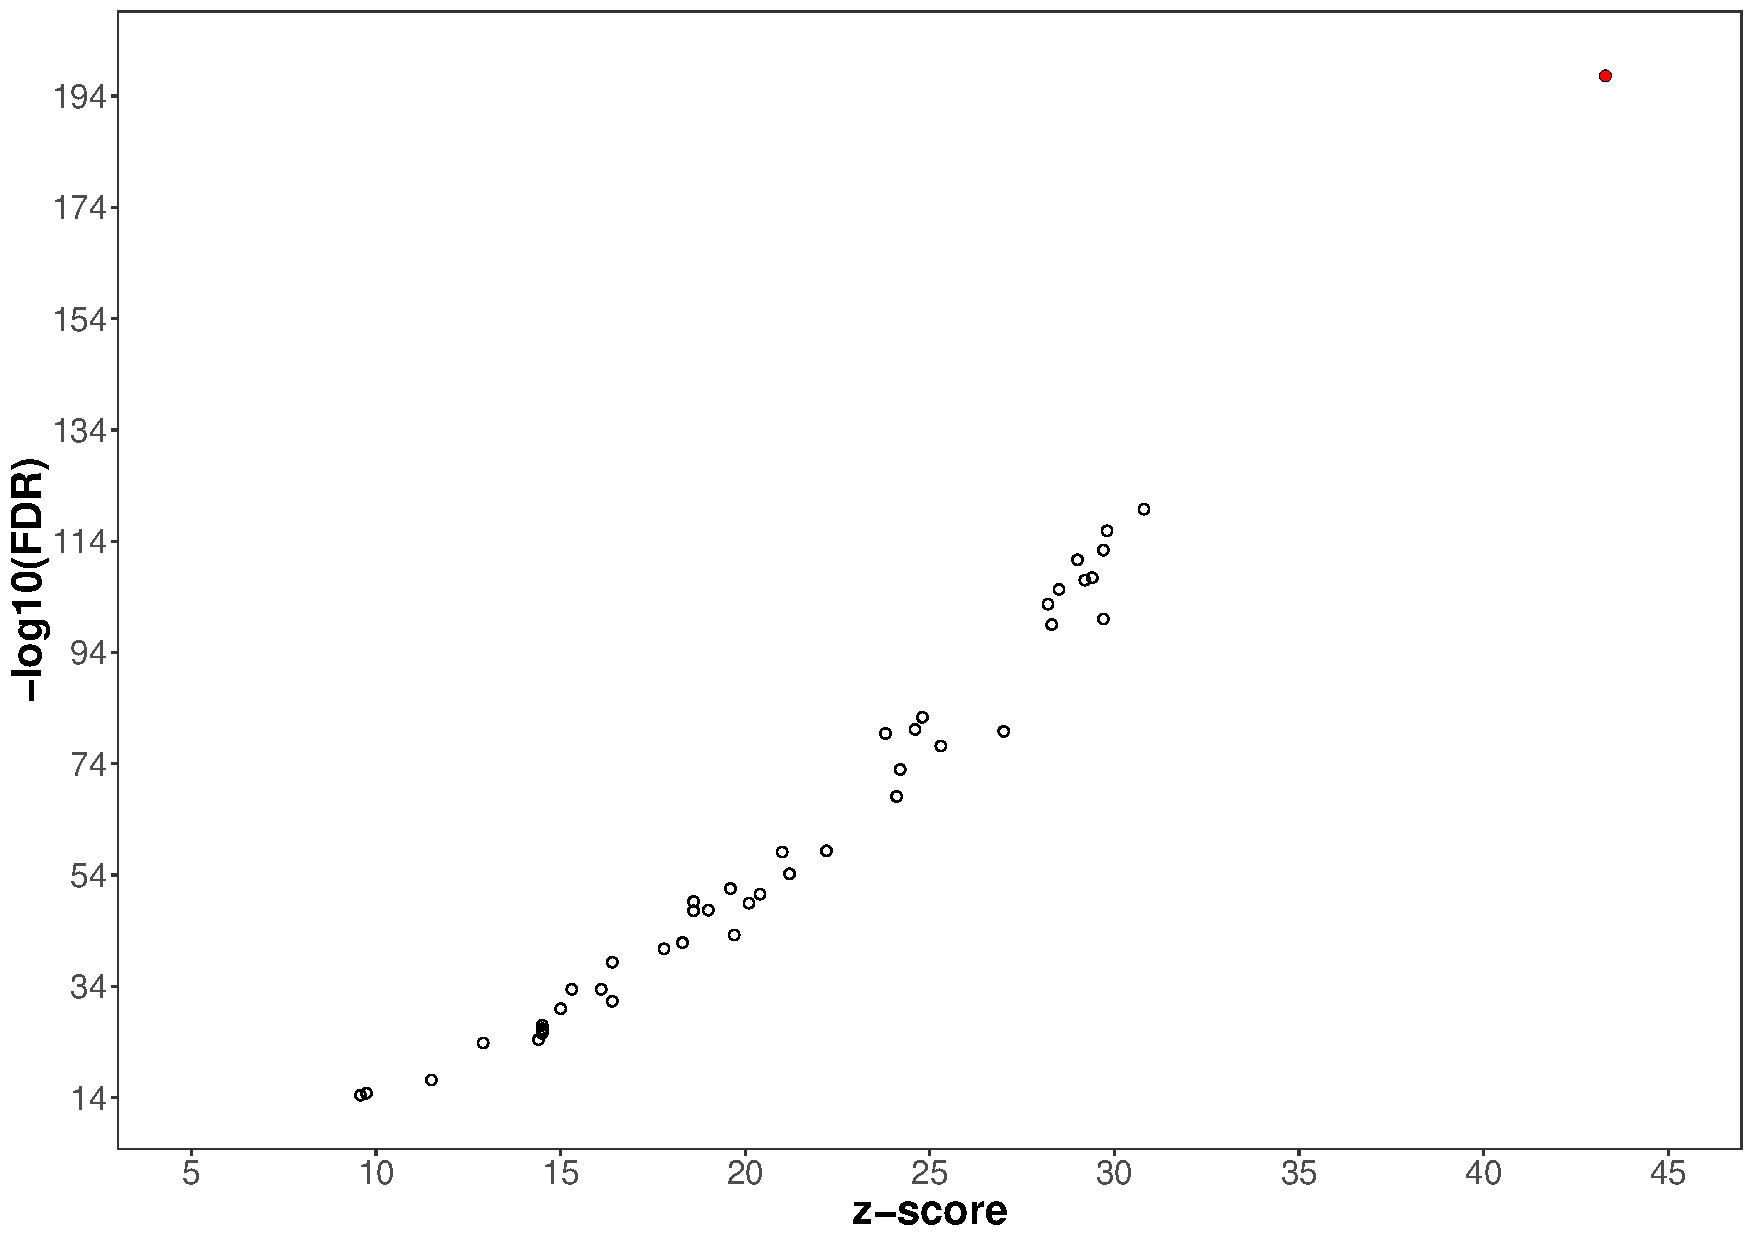
\includegraphics[width=\textwidth]{./Results3/pdfs/ATAC_PSA_all_GTeX_eQTL_enrichment_dotplot}
\caption{}
\end{subfigure}%
\begin{subfigure}[b]{0.5\textwidth} 
%the [b] prevents offset in subcaptions
\centering
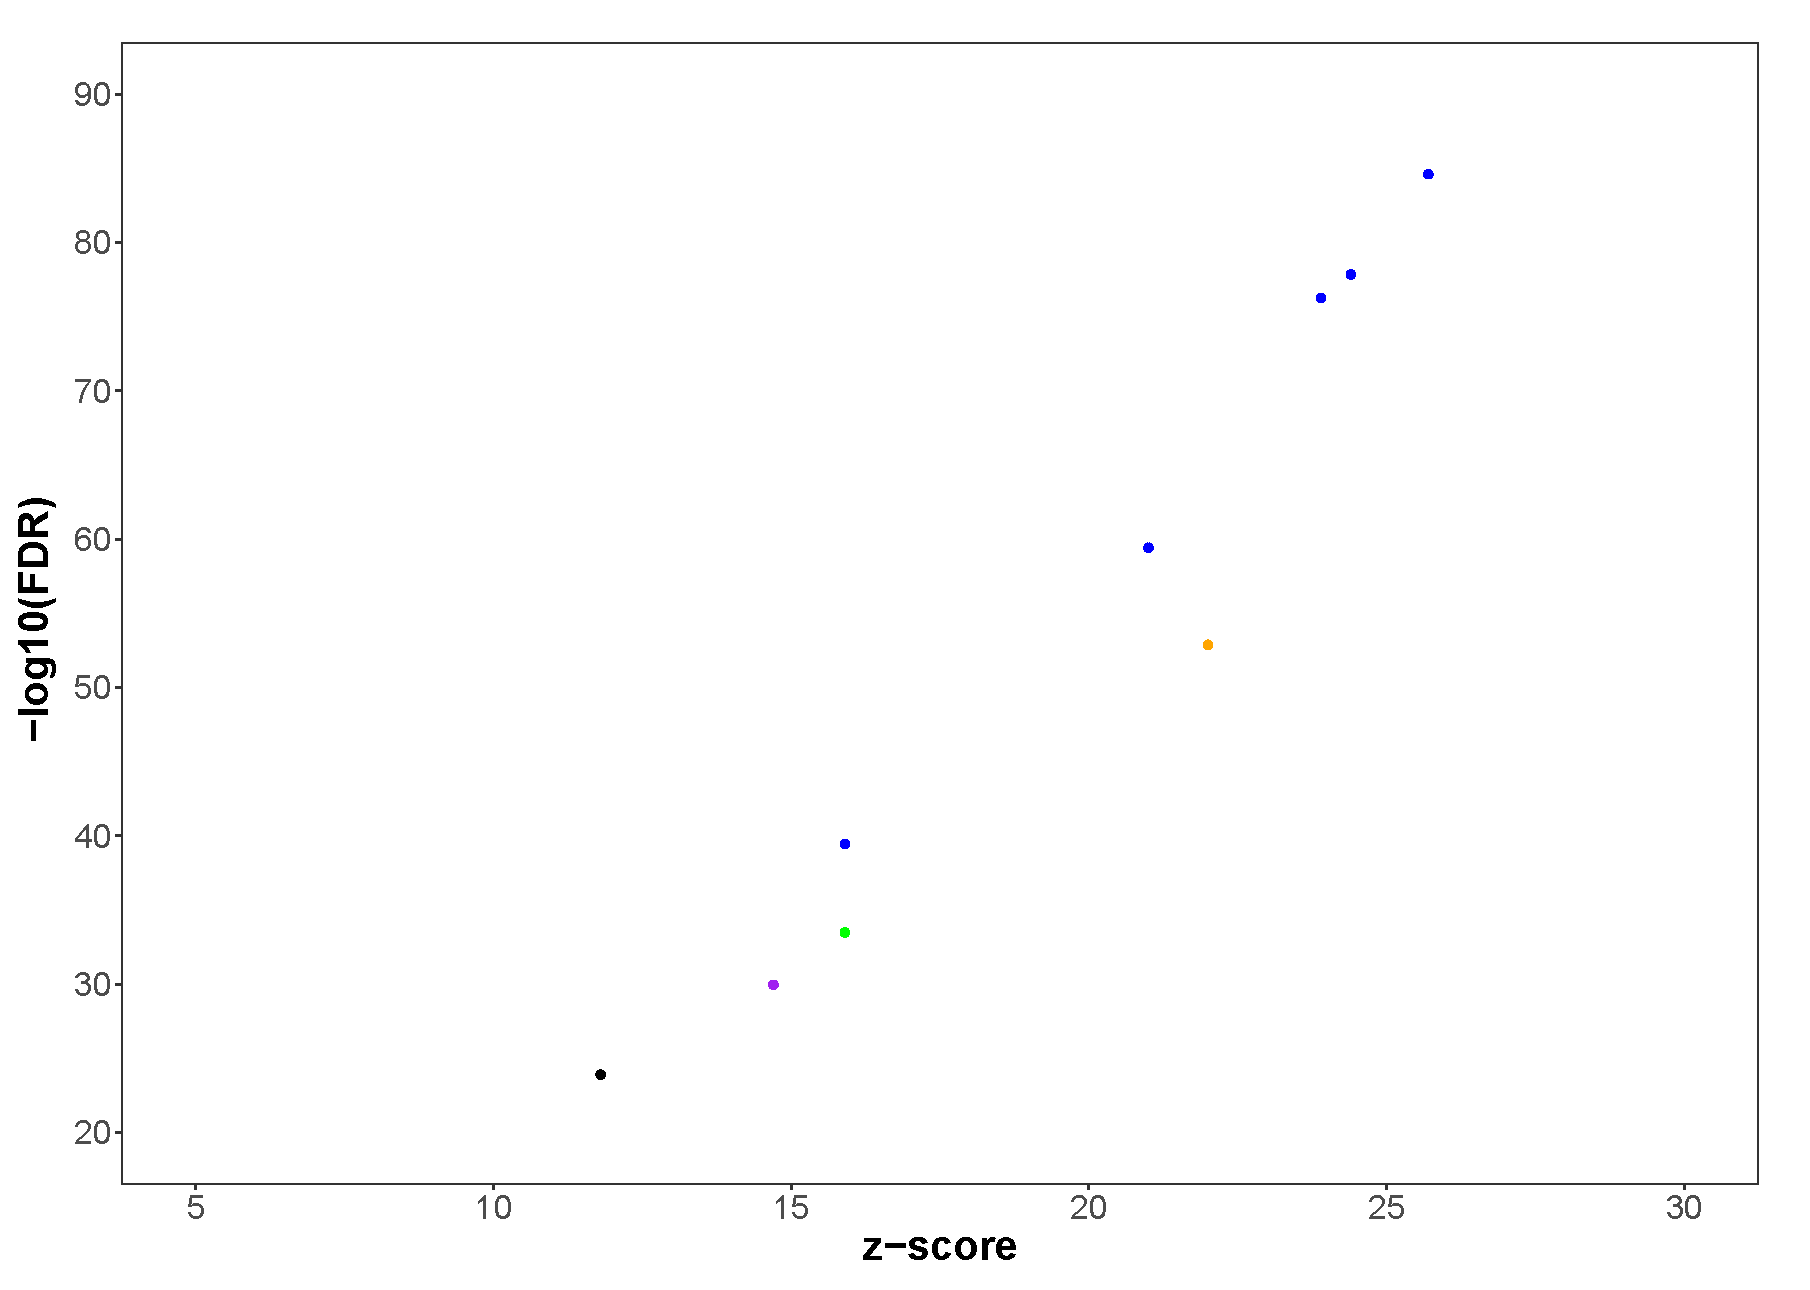
\includegraphics[width=\textwidth]{./Results3/pdfs/ATAC_PSA_all_Jknight_eQTL_enrichment_dotplot}
\caption{}
\end{subfigure}
\caption[Enrichment of eQTLs publicly available data in the combined cell type and tissue chromatin accessibility master list for the PsA cohort.]{\textbf{Enrichment of eQTLs publicly available data in the combined cell type and tissue chromatin accessibility master list for the PsA cohort.} The dot plots showed the z-score values of the enrichment analysis in the x-axis and the significance (-log${_10}$FDR) in the y-axis for a) GTEx eQTL datasets and b) non-GTEx immune-related cell types including CD14$^+$ monocytes (unstimulated, LPS 2h, LPS 24h and 24h IFN$\gamma$ stimulated), B cells, tCD4$^+$, tCD8$^+$ and neutrophils. Dots are colour-coded by cell type.}
\label{figure:PsA_FAST_ATAC_eQTL_enrichment}
\end{figure}



\subsubsection{CD14$^+$ monocytes present the greatest proportion of changes in chromatin accessibility}
A consensus master list of chromatin accessible regions was built for each of the four cell types of interest (ML\_CD14, ML\_CD4, ML\_CD8 and ML\_NK). Differential chromatin accessibility analysis between SF and PB was performed on the normalised counts retrieved for each of the cell type master lists using DESeq2 and a paired design (Table \ref{tab:PSA_DOCs_results}). A 80\% cut-off for background noise was used to filter the count matrix, as previously explained in Chapter \ref{Results3}. %Only differentially accessible regions (DARs) identified with DESeq2 and also shared with quantile normalisation limma voom analysis where considered downstream. 
The CD14$^+$ monocytes and NK were the two cell types presenting the greatest total number (5,285 and 2,314, respectively) and proportion of DARs (23.3 and 8.9\%, respectively). For each cell type, DARs were divided in DARs more open in SF compared to PB (SF open DARs) and DARs less open in SF compared to PB (PB open DARs). In CD14$^+$ monocytes the number of SF open DARS were notably larger than the number of PB open DARs (3,779 and 1,506DARs, respectively) (Table \ref{tab:PSA_DOCs_results}). Conversely, the number of SF and PB open DARs were similar for the other three cell types.


\begin{table}[htbp]
%\setlength{\tabcolsep}{20pt} only to stretch the columns if you want
%\renewcommand{\arraystretch}{1.5}
\centering
\begin{tabular}{@{}c c c c c}
\toprule
\textbf{Cell type}  & \textbf{Total DARs} &  \textbf{Proportion}  & \textbf{SF open} & \textbf{PB open} \\
                    &                     &  \textbf{DARs (\%)}  & \textbf{DARs} & \textbf{DARs} \\
\midrule
\midrule
CD14$^+$ & 5,285 & 23.3 & 3,779 & 1,506 \\
CD4$^+$  & 1,329 & 4.3 & 621 & 708 \\
CD8$^+$  & 1,570 & 4.5 & 807 & 763 \\
NK       & 2,314 & 8.9 & 1,223 & 1,091 \\
\bottomrule
\end{tabular}
\medskip %gap
\caption[Summary results of the differential chromatin accessibility analysis between SF and PB in PsA samples.]{\textbf{Summary results of the differential chromatin accessibility analysis between SF and PB in PsA samples.} For each of the cell types the total number of DARs and the proportion represented by DARs over all the regions included in the differential analysis are reported. The total number of DARs are further divided in those more accessible in SF (DARs open in SF) when compared to PB and those less accessible in SF when compared to PB (DARs open in PB).}
\label{tab:PSA_DOCs_results}
\end{table}

Permutation analysis was used to determine if the large number of DARs (particularly by comparison to limited finding in the psoriasis analysis) were more than would be expected by chance. None of the ten possible permutations demonstrated a greater number of DARs than the ones identified for the true groups, reinforcing the robustness of the differential analysis results (Figure \ref{figure:PsA_perm_analysis}).

  
Genomic annotation of the DARs identified in each the cell types revealed that 80\% or more of all regions with differential accessibility were located at intronic and intergenic regions (Figure \ref{figure:PsA_FAST_ATAC_DOCS_annotation} a). Universal promoter regions was the third most represented genomic feature, accounting for the annotation of approximately between 5 to 15\% of the DARs in each cell type. In addition to this, the chromatin states from the Roadmap Epigenomics maps were also used for annotation (Figure \ref{figure:PsA_FAST_ATAC_DOCS_annotation} b). For all four cell types,  between 44.96 and 72.11\% of the DARs were annotated as weak enhancers, which represented the most prominent category and the most significantly enriched (data not shown). The over-representation of enhancers was consistent with large percentage of introns and intergenic regions found for the genomic features annotation, as those are the preferred location for enhancer elements. Modest percentages of DARs were annotated as heterochromatin and repetitive regions but not significant enrichment for these two chromatin states was found for any of the four cell types (Figure \ref{figure:PsA_FAST_ATAC_DOCS_annotation} b).
%

\bigskip
\begin{figure}[H]
\centering
\begin{subfigure}[b]{0.5\textwidth}
\centering 
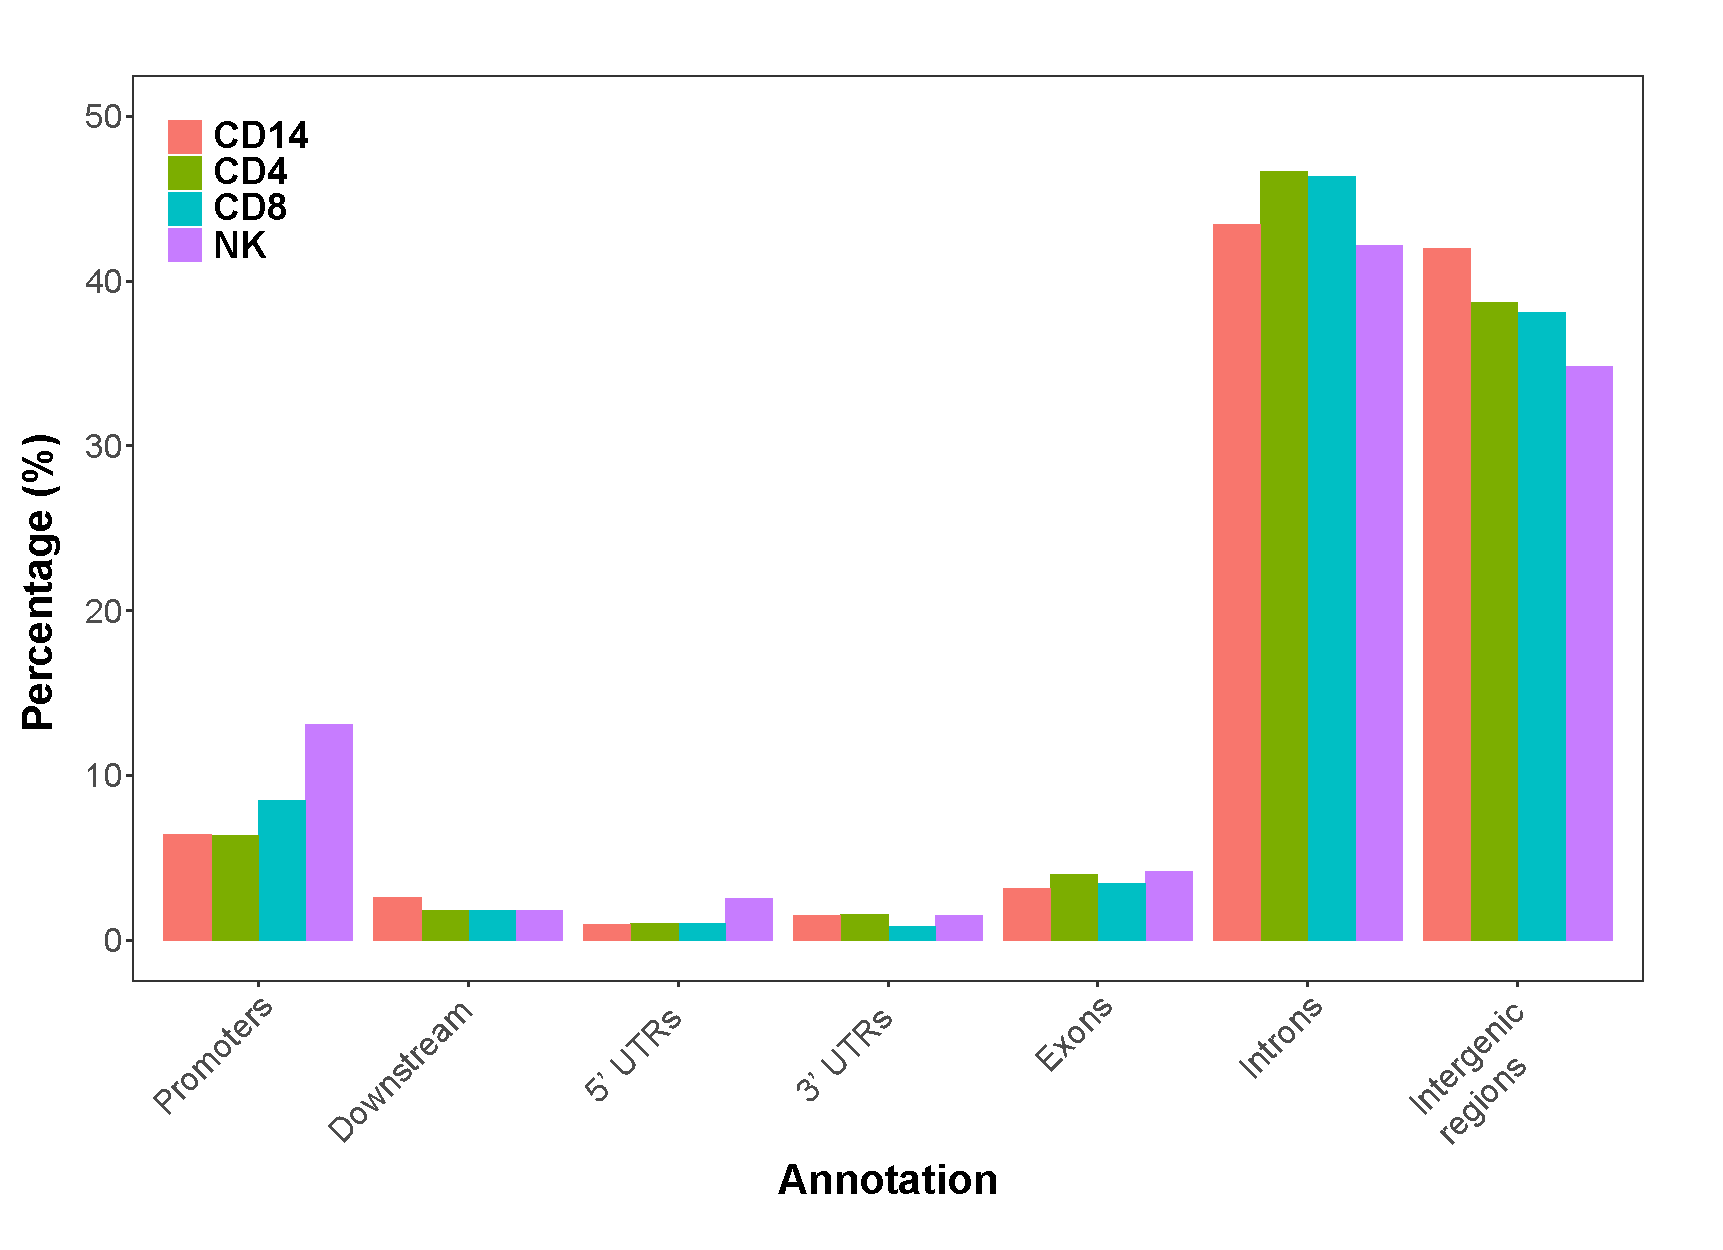
\includegraphics[width=\textwidth]{./Results3/pdfs/ATAC_PSA_DOCS_per_cell_type_general_annotation}
\caption{}
\end{subfigure}
~
\begin{subfigure}[b]{0.6\textwidth} 
%the [b] prevents offset in subcaptions
\centering
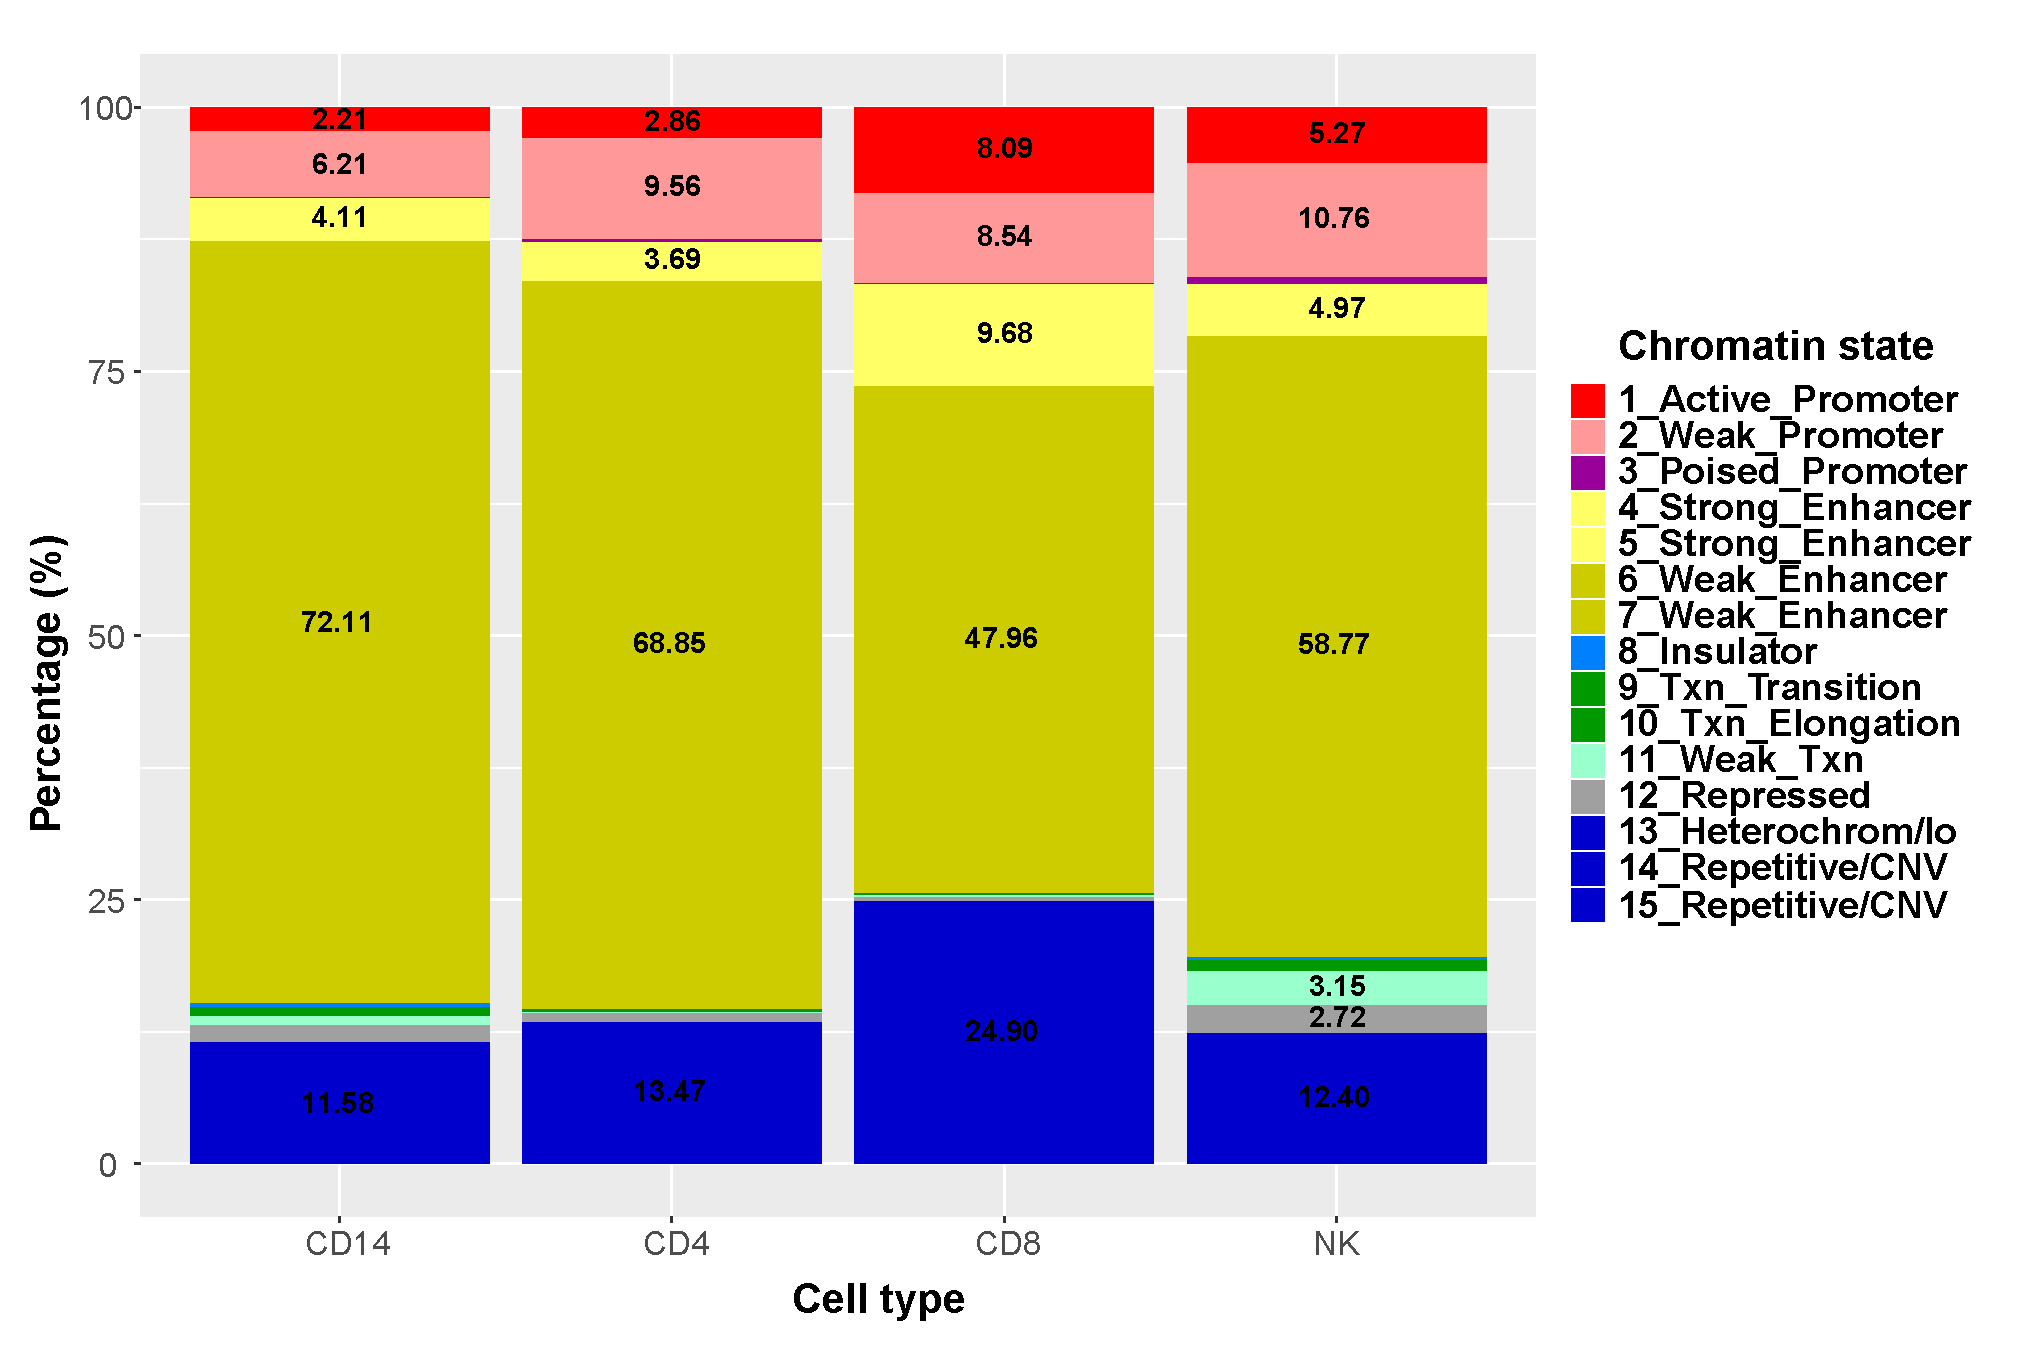
\includegraphics[width=\textwidth]{./Results3/pdfs/ATAC_PSA_DOCS_chromatin_states_stacked_barplot}
\caption{}
\end{subfigure}
\caption[Annotation of the PsA DARs identified in the four cell types with genomic annotations and chromatin states.]{\textbf{Annotation of the PsA DARs identified in the four cell types with genomic annotations and chromatin states.} a) Barplot illustrating the percentage of nucleotides within DARs for each cell type that are annotated as promoters, downstream (regions at $\leq$1,000bp to a promoter), exons, introns, 5' or 3'UTR and intergenic regions. b) Stacked barplot representing the percentage of DARs annotated for each of the fifteen chromatin states defined in each of the four relevant cell types by Epigenome Roadmap chromatin segmentation maps (CD14$^+$ PB isolated monocytes, mCD4$^+$, mCD8$^+$ and NK cells).}
\label{figure:PsA_FAST_ATAC_DOCS_annotation}
\end{figure}


%Try to overlap the enhancer FANTOM data to id those regions whith evidence of eRNA expression
The functional relevance of the differential chromatin accessibility in terms of regulation of gene expression was further investigated by integration of the eRNA data from the FANTOM5 project. Statistically significant enrichment for robust and permissive enhancers was found for the DARs in all four cell types (Figure \ref{figure:PSA_FANTOM}).  Moreover, DARs from all four cell types also presented significant enrichment for the corresponding cell type eRNA set. The proportion of DARs overlapping the appropriate cell type set of expressed eRNAs ranged between 19.8\% (83 open in SF and 160 open in PB) in NK and 31.8\% (83 open in SF and 160 open in PB) in CD4$^+$ cells.


\begin{figure}[htbp]
\centering
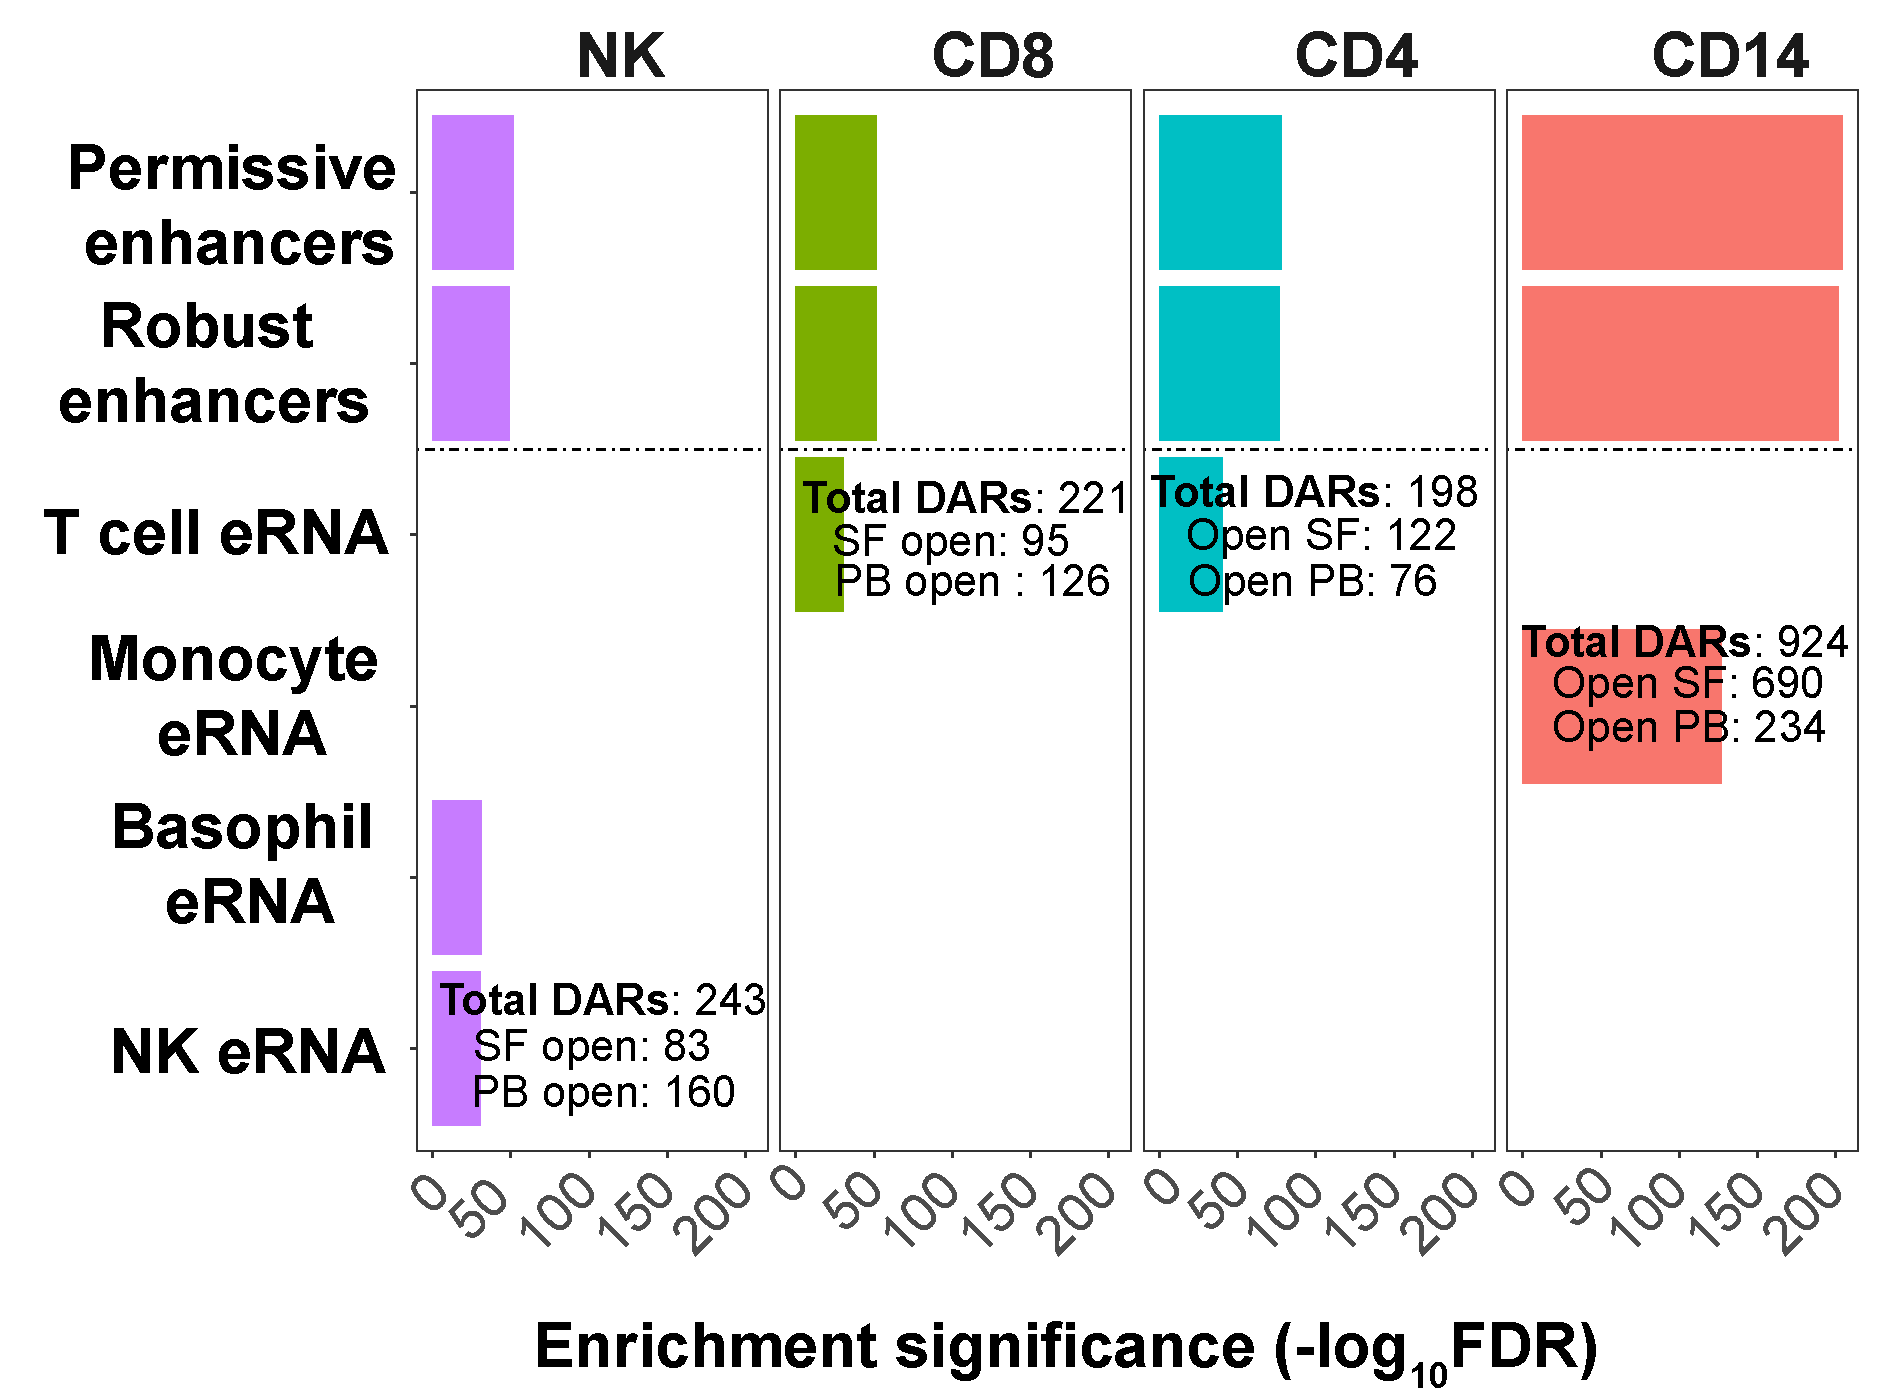
\includegraphics[width=0.6\textwidth]{./Results3/pdfs/ATAC_PsA_FANTOM_enhancer_enrichment_all_cell_types}
\caption[Enrichment of PsA DARs for the FANTOM5 eRNA dataset.]{\textbf{Enrichment of PsA DOCs for the FANTOM5 eRNA dataset.} Robust enhancers have been defined as those detected at the genome-wide significant level in at least one primary cell type or tissue. Permissive enhancers are all detected eRNAs but not passing genome-wide filtering criteria \parencite{Andersson2014}. Robust enhancers represent a subset of the permissive enhancers. Significance is considered for FDR$<$0.01.}
\label{fig:PSA_FANTOM}
\end{figure}

From the differential analysis between SF and PB, a number of DARs were overlapping a gene body (Table \ref{tab:PSA_DOCs_gene_body}). Interestingly, the majority were located within introns instead of untranslated regions (UTRs) annotated as weak or strong enhancers according to the cell type specific chromatin segmentation map previously illustrated. 

%Similarly, more accessible chromatin in SF compared to PB was identified in five regions of the \textit{IL15} gene, annotated as promoter and enhancers in CD14$^+$ monocytes. 
% Check differences at both gene locations were CD14$^+$ cell type specific is this region HiC annotated with the gene? and maybe include example overlapping eRNA
%e.g LMNA4 which is CD14 cell specific and more expressed in SF in Dolcino paper. Maybe use it later

\begin{table}[htbp]
%\setlength{\tabcolsep}{20pt} only to stretch the columns if you want
%\renewcommand{\arraystretch}{1.5}
\centering
\begin{tabular}{@{} c c c c c}
\toprule
\textbf{Cell type} & \textbf{DARs in} &  \textbf{Gene with more}     &\textbf{Enhancers} & \textbf{Introns} \\
                   & \textbf{gene body} &  \textbf{than one one DAR} &                   &                   \\
\midrule
\midrule
CD14$^+$ & 2,357 & 744 & 1,775 & 1,920 \\
CD4$^+$ & 700 & 99 & 504 & 577 \\
CD8$^+$ & 831 & 118 & 503 & 666 \\
NK   & 1,246 & 235 & 782 & 937 \\   
\bottomrule
\end{tabular}
\medskip %gap
\caption[Characterisation of the DARs located within genes in each of the four cell types from PsA samples.]{\textbf{Characterisation of the DARs located within genes in each of the four cell types from PsA samples.} The numbver of DARs that overlapping a gene body for each of the cell types are indicated together with those genes harbouring more than one DARs. Further details about those regions includes specification of the number located at introns and those annotated as enhancers according to the Epigenome Roadmap chromatin segmentation maps of each appropriate cell type.}
\label{tab:PSA_DOCs_gene_body}
\end{table}

For example, NK analysis identified a PB open DAR located in an intron of the \textit{VAV3} gene and also significantly expressed as eRNA (Figure \ref{figure:PsA_FAST_ATAC_gene_boy_DOCS_CD14_NK} a). Additionally, a number of gene entities contained more than one DAR, showing the same direction of chromatin accessibility between SF and PB. For example, in CD14$^+$ two DARs located at the 5' and 3' UTRs of \textit{IL7R} gene were more accessible in SF compared to PB (Figure \ref{figure:PsA_FAST_ATAC_gene_boy_DOCS_CD14_NK} b). 

\bigskip
\begin{figure}[H]
\centering
\begin{subfigure}[b]{0.60\textwidth}
\centering 
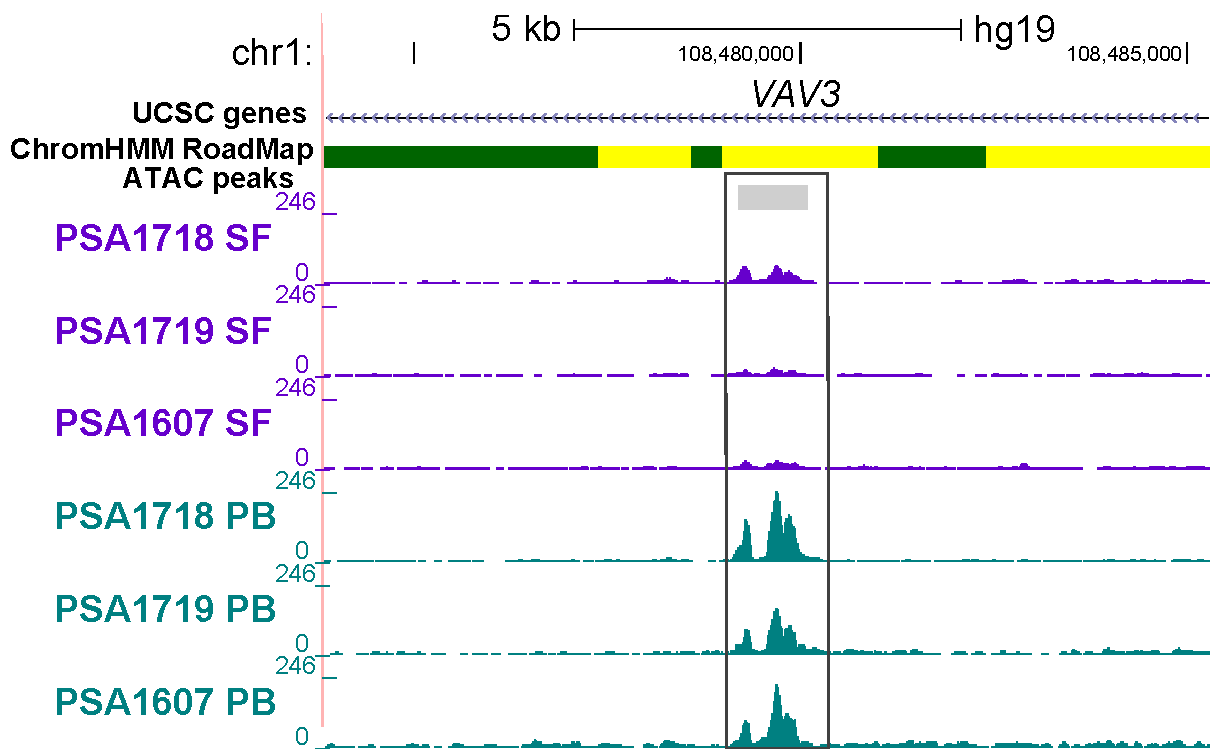
\includegraphics[width=\textwidth]{./Results3/pdfs/ATAC_PSA_NK_VAV3}
\caption{}
\end{subfigure}
~
\begin{subfigure}[b]{0.60\textwidth} 
%the [b] prevents offset in subcaptions
\centering
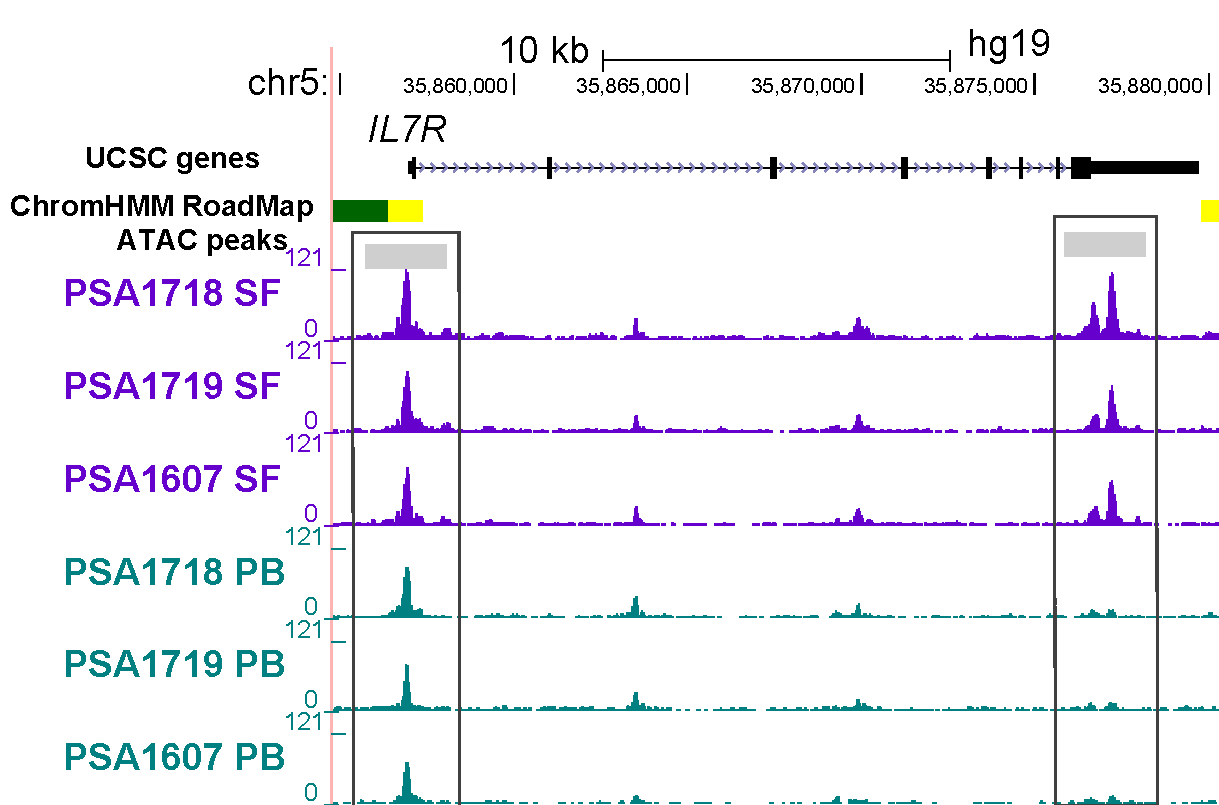
\includegraphics[width=\textwidth]{./Results3/pdfs/ATAC_PSA_CD14_IL7R}
\caption{}
\end{subfigure}
\caption[Differentially accessible regions located within gene bodies in CD14$^+$ monocytes and NK cells from PsA patients.]{\textbf{Differentially accessible regions located within gene bodies in CD14$^+$ monocytes and NK cells from PsA patients.} UCSC Genome Browser view illustrating the normalised ATAC read density (y-axis) in a) DAR located at an intron of \textit{VAV3} gene (x-axis) in NK (less accessible in SF compared to PB) and b) two DARs mapping to the 5' and 3'UTR of the \textit{IL7R}, respectively, in CD14$^+$ monocytes (both more accessible in SF compared to PB). Tracks are colour-coded by tissue (SF=purple and PB=turquoise). The Epigenome Roadmap chromatin segmentation track for the appropriate cell type are also shown. All DARs were significant based on FDR$<$0.01 and FC$>$1.5.}
\label{figure:PsA_FAST_ATAC_gene_boy_DOCS_CD14_NK}
\end{figure}



% GWAS overlap maybe indicate an example in CD14 that can be relevant with pathway analysis
%The relevance of the differences in chromatin accessibility in the context of psoriasis and PsA GWAS hits was also addressed. Enrichment analysis of psoriasis and PsA GWAS hits for the DARs in each cell type was performed using XGR co-localisation and permutation analysis. At the SNP level, no significant enrichment was reported between DARs and GWAS lead SNPs and those in LD r$^2$$\geq$8. When the enrichment analysis was performed for the psoriasis and PsA LD blocks, significant enrichment (2-fold enrichment and empirical p-val 0.043) was observed only for the CD14$^+$ DARs.

In all four cell types, overlap between putative psoriasis and PsA GWAS genes and proximal ($\leq$5Kb) DARs were found. CD14$^+$ monocytes presented the largest number of overlaps (12), followed by mCD8$^+$ (9), NK$^+$ (8) and mCD4$^+$ (4). For example, DARs proximal to \textit{ELMO1} and \textit{RUNX3} were found for all the cell types. Co-localisation and permutation analysis to explore the enrichment of DARs for PsA and psoriasis GWAS LD blocks only found significance in CD14$^+$ monocytes (empirical pval=0.043).

\subsection{Pathway enrichment analysis highlights tissue functional differences in chromatin accessibility}

Pathway enrichment analysis was conducted separately for SF open DARs and PB open DARs in each cell type. Gene annotation of the DARs was performed by physical proximity, as detailed in Chapter \ref{ch:Mat}. Despite commonalities, differences in significant enriched pathways (FDR$<$0.01 or 0.05) were also identified within the same cell type between SF and PB open DARs (Figure \ref{figure:PSA_ATAC_pathway_analysis_all_DOC}). In CD14$^+$ monocytes SF open DARs presented enrichment for pathways involved in regulation of immunity, inflammation and cell survival such as the NF-$\kappa$B pathway and cytokine related pathways, including IL-2 and IL-3, 5 and granulocyte-macrophage colony–stimulating factor (GM-CSF) signalling (Figure \ref{figure:PSA_ATAC_pathway_analysis_all_DOC} a). 

mCD4$^+$ SF open DARs compared to PB open DARs showed enrichment for TCR signalling as well as chemokine signalling, which included, amongst others, DARs in proximity to IFN-$\gamma$ or \textit{CXCL13} and \textit{CXCR6}, respectively (Figure \ref{figure:PSA_ATAC_pathway_analysis_all_DOC} b). T cell signaling pathway appeared only enriched for SF open DARs in mCD4$^+$; however PB open DARs in this cell type were also enriched for focal adhesion members, also involved in the T cell activation \parencite{Dustin2001}. Enriched pathways for SF or PB open DARs in mCD8$^+$ were only significant when using an FDR$<$0.05 threshold. (Figure \ref{figure:PSA_ATAC_pathway_analysis_all_DOC} c). The G protein coupled receptor (GPCR) signalling, with varied roles in regulation of inflammation and mediation of the chemotactic recruitment of T cells to the inflamed tissue, was enriched for mCD8$^+$ PB open DARs. mCD8$^+$ SF open DARs showed enrichment for the Wnt signaling pathway involved in the production of memory cells with enhanced proliferative potential and stronger protective capacity \parencite{Boudousquie2014,}. 

NK SF open DARs presented enrichment for Fc-gamma receptor (FC$\gamma$R)-mediated phagocytosis (Figure \ref{figure:PSA_ATAC_pathway_analysis_all_DOC} d). Moreover, members of the HIF-1 pathway involved in oxygen homeostasis were also enriched in NK SF open DARs, in line with the hypoxic environment found in joint inflammation. Interestingly, enrichment of open PB DARs in the proximity of genes involved in NK-mediated toxicity was unveiled. 
% NK CD56 bright subsets and tissue http://www.jimmunol.org/content/196/7/2923.long
% Production of IgG in PsA http://www.jrheum.org/content/41/12/2421.long
% NK phagocytisis FCgamma R III https://www.ncbi.nlm.nih.gov/pmc/articles/PMC1550276/, https://www.sciencedirect.com/science/article/pii/S0022202X15300373#bb0030, https://www.sciencedirect.com/science/article/pii/S0022202X15300373#bb0185
%Joint hypoxia https://www.ncbi.nlm.nih.gov/pmc/articles/PMC3683428/
%Skin hypoxia https://www.sciencedirect.com/science/article/pii/S0022202X15331328?via%3Dihub

\begin{figure}[H]
\centering
\begin{subfigure}[b]{0.45\textwidth}
\centering 
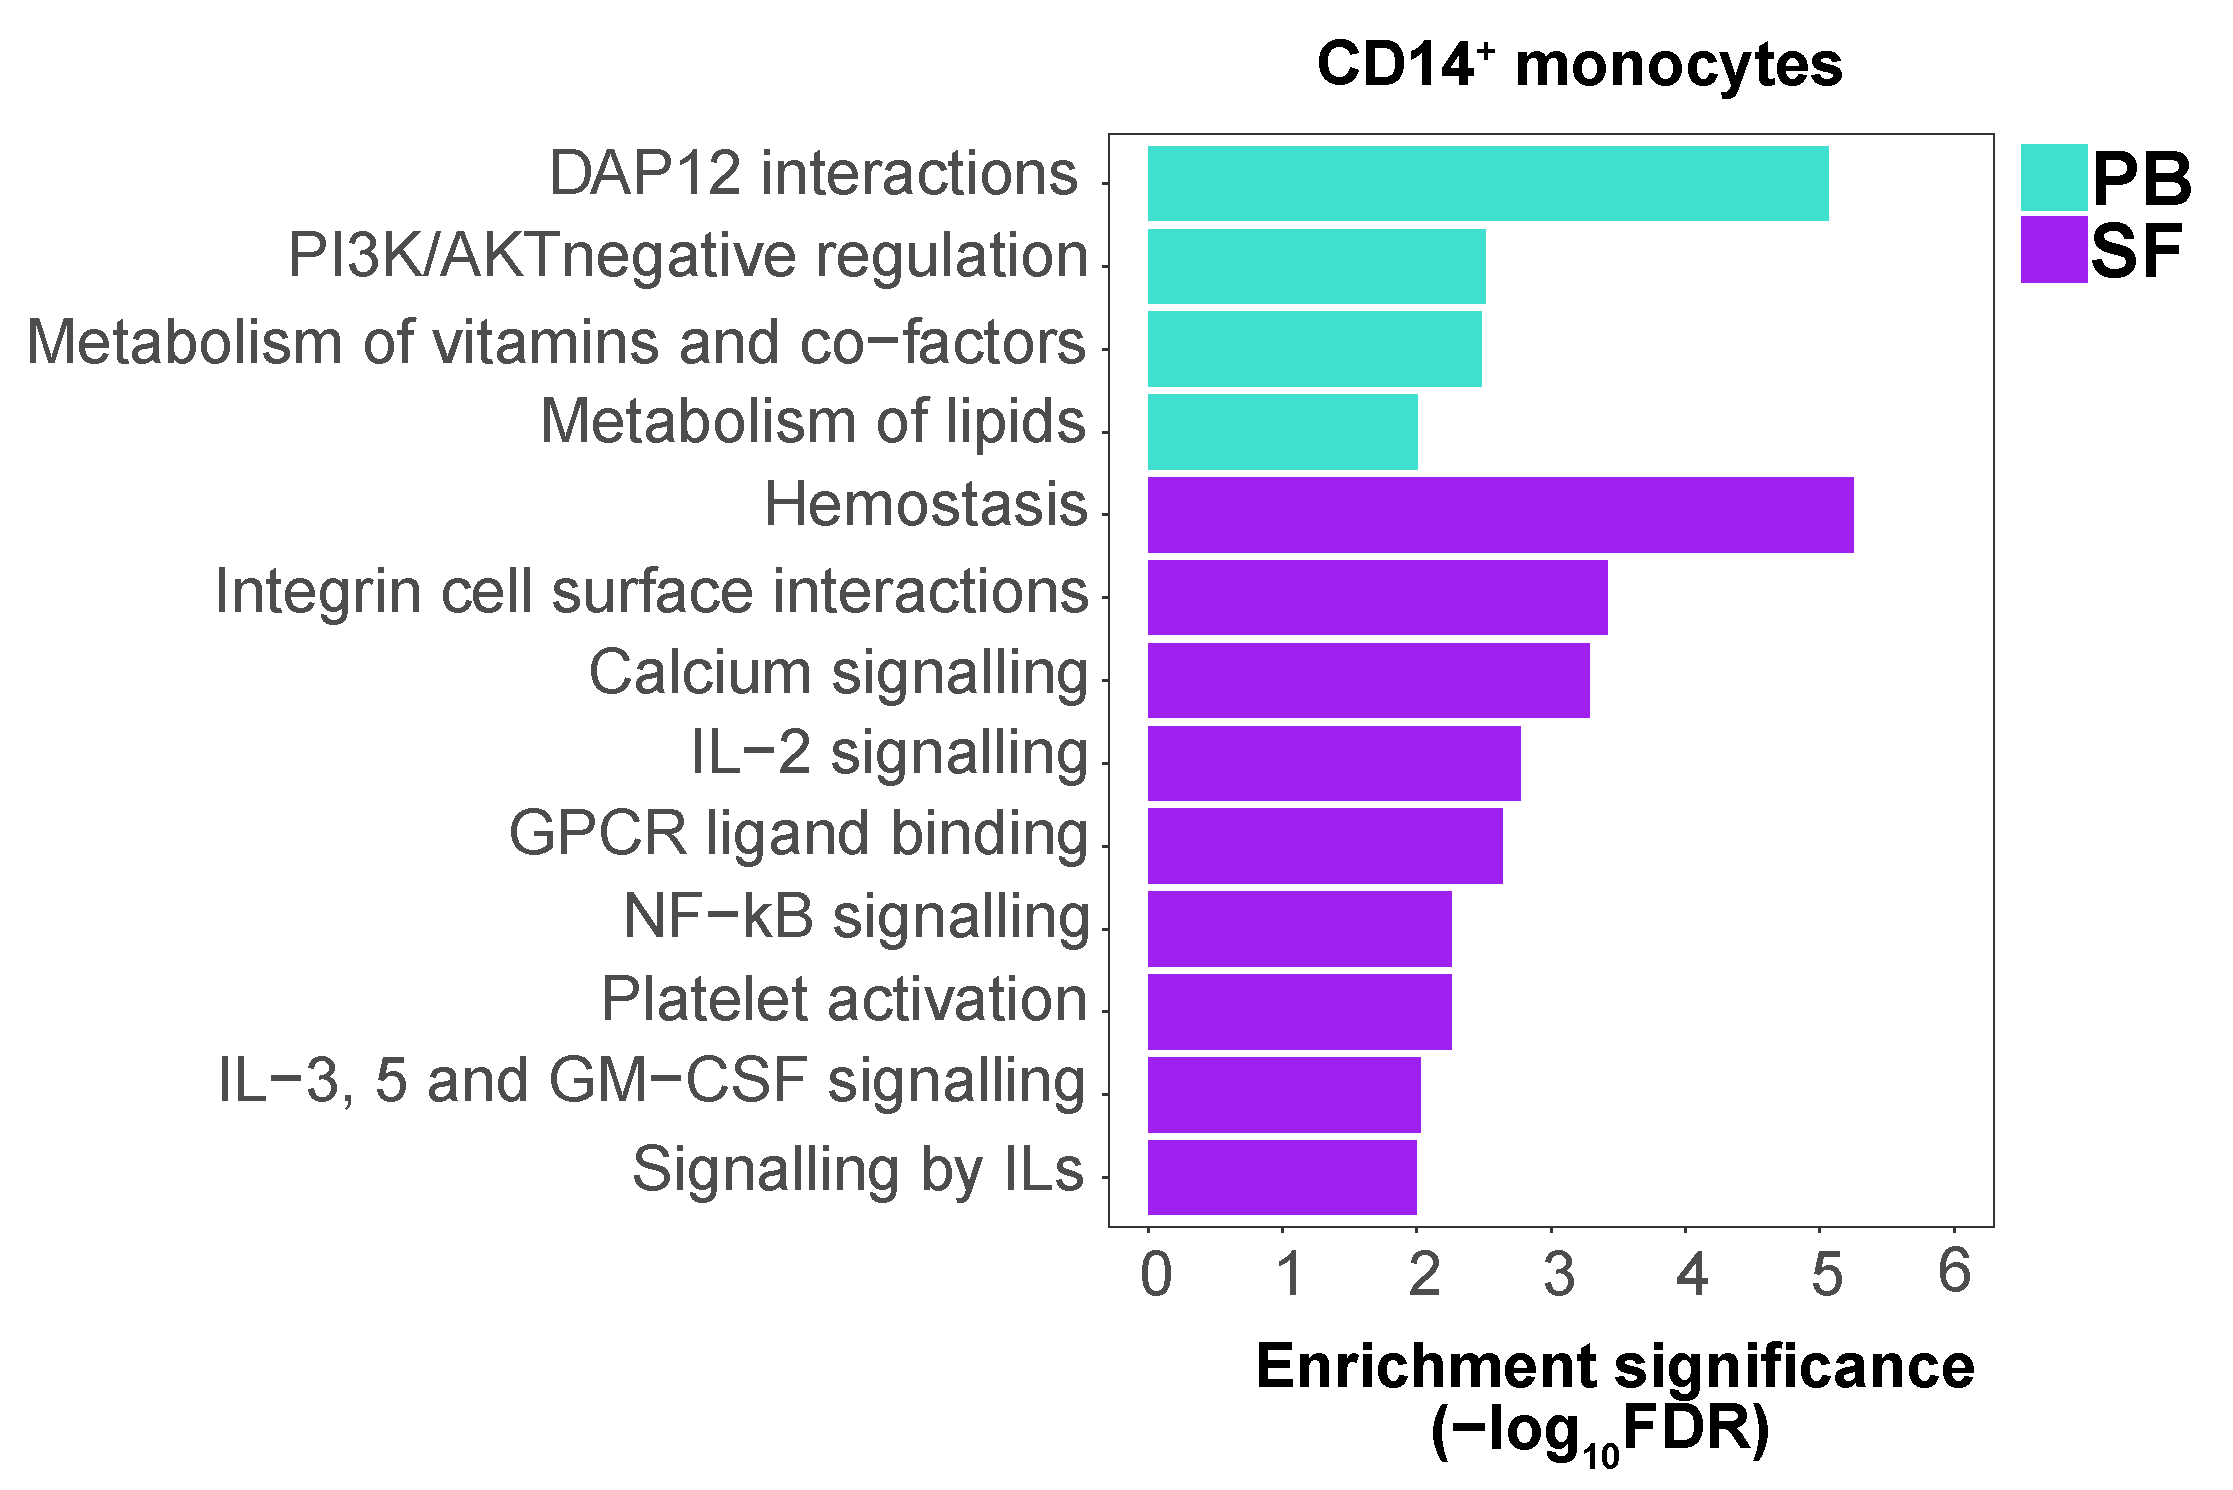
\includegraphics[width=\textwidth]{./Results3/pdfs/ATAC_PSA_CD14_pathways_barplot_all_DOCS_proximity}
\caption{}
\end{subfigure}
~
\begin{subfigure}[b]{0.45\textwidth}
\centering 
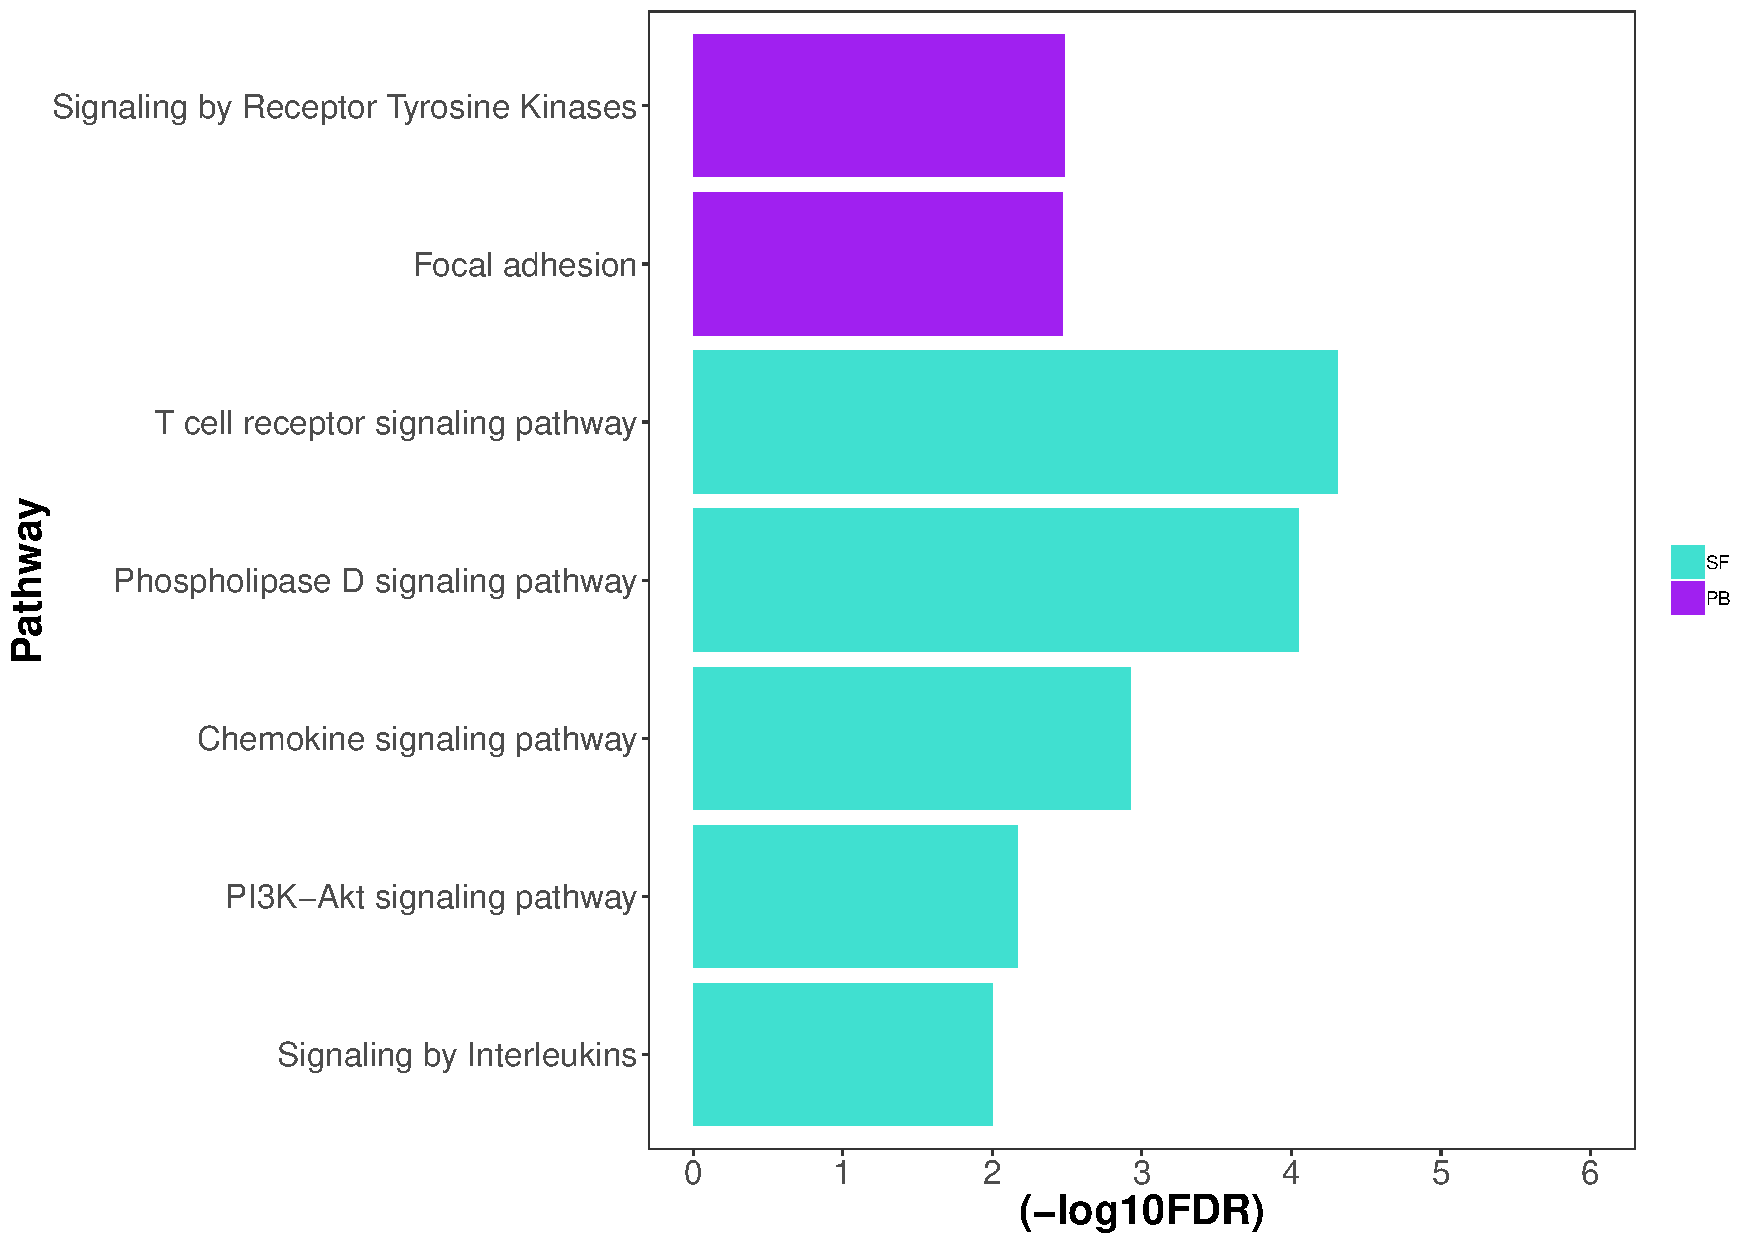
\includegraphics[width=\textwidth]{./Results3/pdfs/ATAC_PSA_CD4_pathways_barplot_all_DOCS_proximity}
\caption{}
\end{subfigure}
~
\begin{subfigure}[b]{0.45\textwidth} 
%the [b] prevents offset in subcaptions
\centering
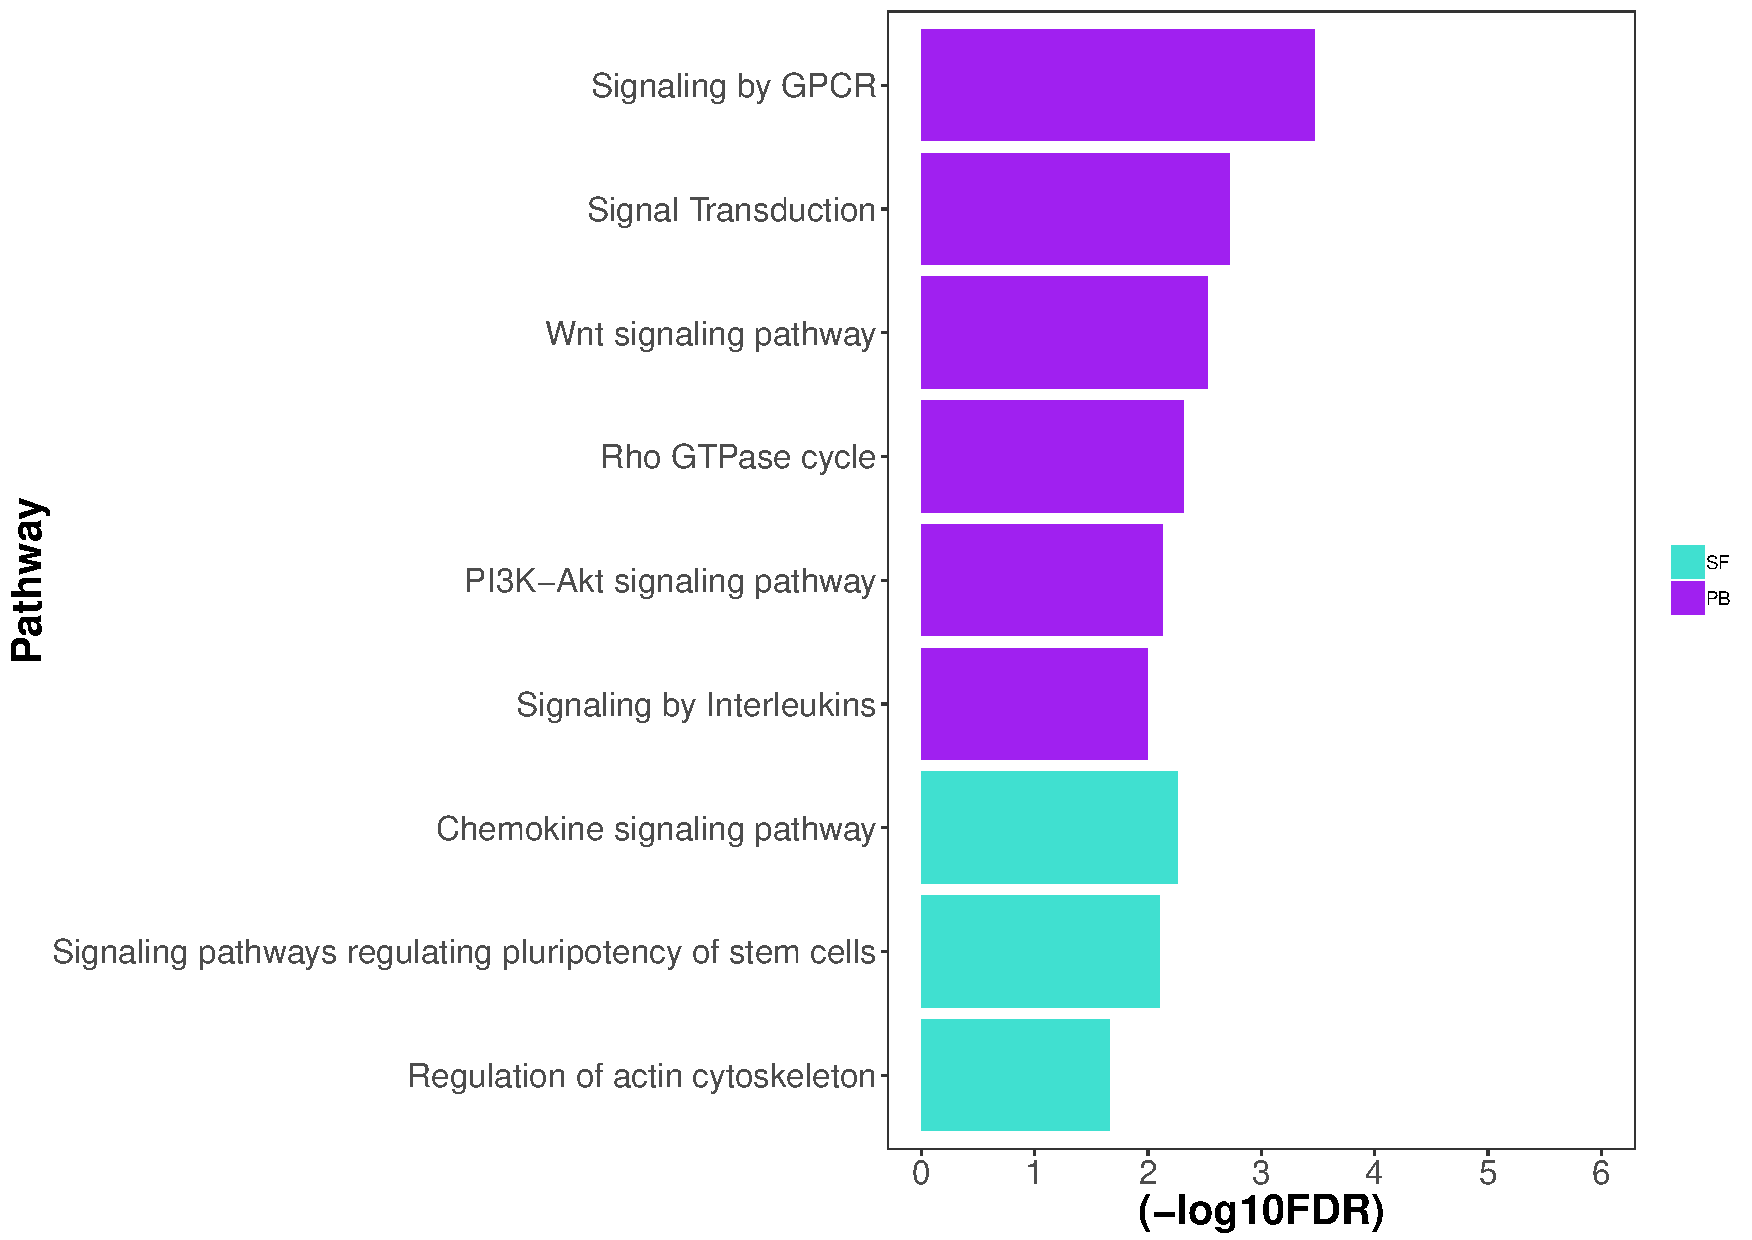
\includegraphics[width=\textwidth]{./Results3/pdfs/ATAC_PSA_CD8_pathways_barplot_all_DOCS_proximity}%
\caption{}
\end{subfigure}
\begin{subfigure}[b]{0.45\textwidth} 
%the [b] prevents offset in subcaptions
\centering
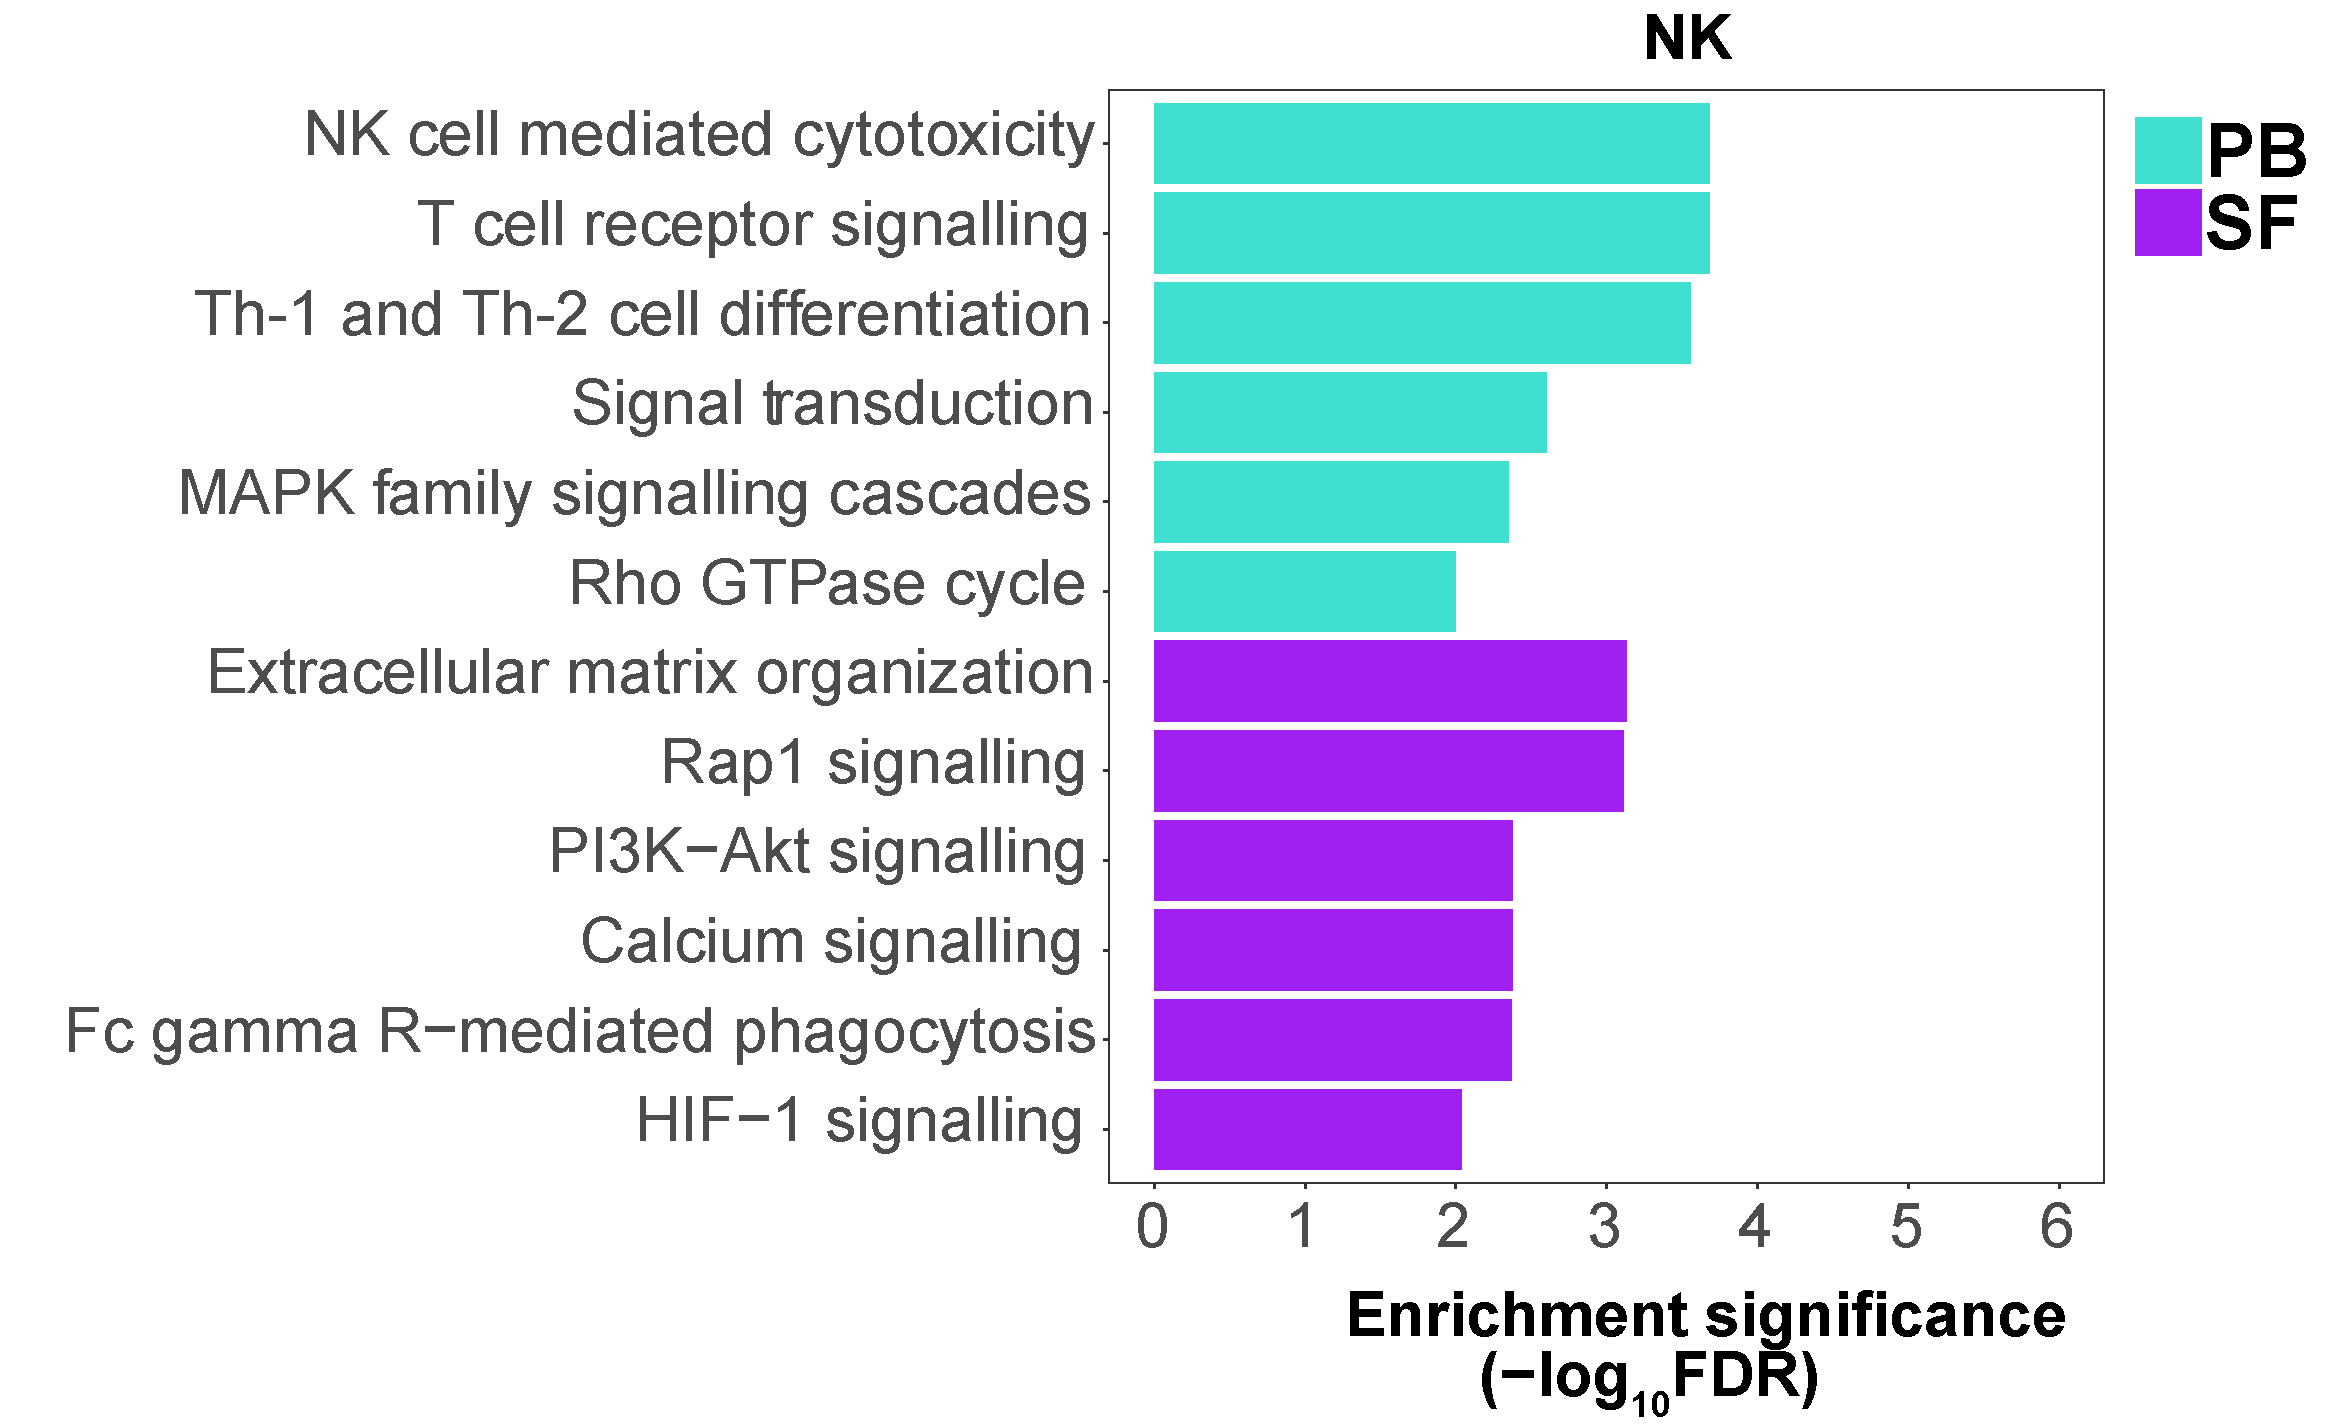
\includegraphics[width=\textwidth]{./Results3/pdfs/ATAC_PSA_NK_pathways_barplot_all_DOCS_proximity}%
\caption{}
\end{subfigure}
\caption[Distinct functional pathways enriched for DARs open in SF or open in PB in CD14$^+$ monocytes, CD4m$^+$,CD8m$^+$ and NK.]{\textbf{Distinct functional pathways enriched for DARs open in SF or open in PB in CD14$^+$ monocytes, CD4m$^+$,CD8m$^+$ and NK.} Enrichment analysis was performed separately for the DARs open in SF and DARs open in PB separately in a) CD14$^+$ monocytes, b) mCD4$^+$, c) mCD8$^+$ and d) NK. The pathways presenting significant enrichment (FDR $<$0.01) only in open SF or open PB DARs are shown here.}
\label{figure:PSA_ATAC_pathway_analysis_all_DOC}
\end{figure}


%Decide if table or barplots
%\begin{landscape}
%\begin{center}
%\begin{longtable}[ht]{c c c }
%\caption[Distinct enriched pathways in CD14$^+$, mCD4$^+$, mCD8$^+$ and NK between SF and PB]{\textbf{Distinct enriched pathways in CD14$^+$, mCD4$^+$, mCD8$^+$ and NK between SF and PB.} All pathways shown have an FDR $<$0.01.}
%\\
%\label{table:PSA_ATAC_pathway_analysis_all_DOC} \\
%\toprule
%\textbf{Cell type} & \textbf{SF} & \textbf{PB} \\						
%\midrule
%\midrule
%CD14$^+$ & Hemostasis, Platelet activation, Signaling by VEGF & DAP12 interactions, Metabolism of lipids, \\ 
         %& GPCR ligand binding, IL-2 signaling pathway, & Metabolism of vitamins and co-factors, \\ 
         %& Integrin cell surface interactions,NF-kappa B signaling pathway & Negative regulation of the PI3K/AKT network. \\ 
         %& IL-2 family signaling, IL-3, 5 and GM-CSF signaling. & \\ 
%\midrule
%\textbf{mCD4$^+$} & T cell receptor signaling pathway, Phospholipase D signaling pathway ,& Signaling by Receptor Tyrosine Kinases,\\ 
									%& Chemokine signaling pathway, PI3K-Akt signaling pathway, & Focal adhesion.\\ 
									%& Signaling by interleukins. & \\
%\midrule
%\textbf{mCD8$^+$} & Chemokine signaling pathway, Signaling by GPCR  & Signal transduction, Wnt signaling pathway,\\ 
									%& Signaling pathways regulating pluripotency of stem cells & Rho GTPase cycle, PI3K-Akt signaling pathway, \\ 
									%& Regulation of actin cytoskeleton. & Signaling by interleukins. \\ 
%\midrule
%\textbf{NK$^+$} & Extracellular matrix organization, Rap1 signaling pathway, & Th1 and Th2 cell differentiation, Rho GTPase cycle,\\ 		
								%& Calcium signaling pathway, PI3K-Akt signaling pathway,     & T cell receptor signaling pathway, Signal Transduction,\\ 
								%& Fc gamma R-mediated phagocytosis, HIF-1 signaling pathway. & Natural killer cell mediated cytotoxicity,  \\
								%&                                                            & MAPK family signaling cascades.	\\ 								
%\bottomrule
%\medskip
%\end{longtable}
%\end{center}
%\end{landscape}



%\begin{figure}[htbp]
%\centering
%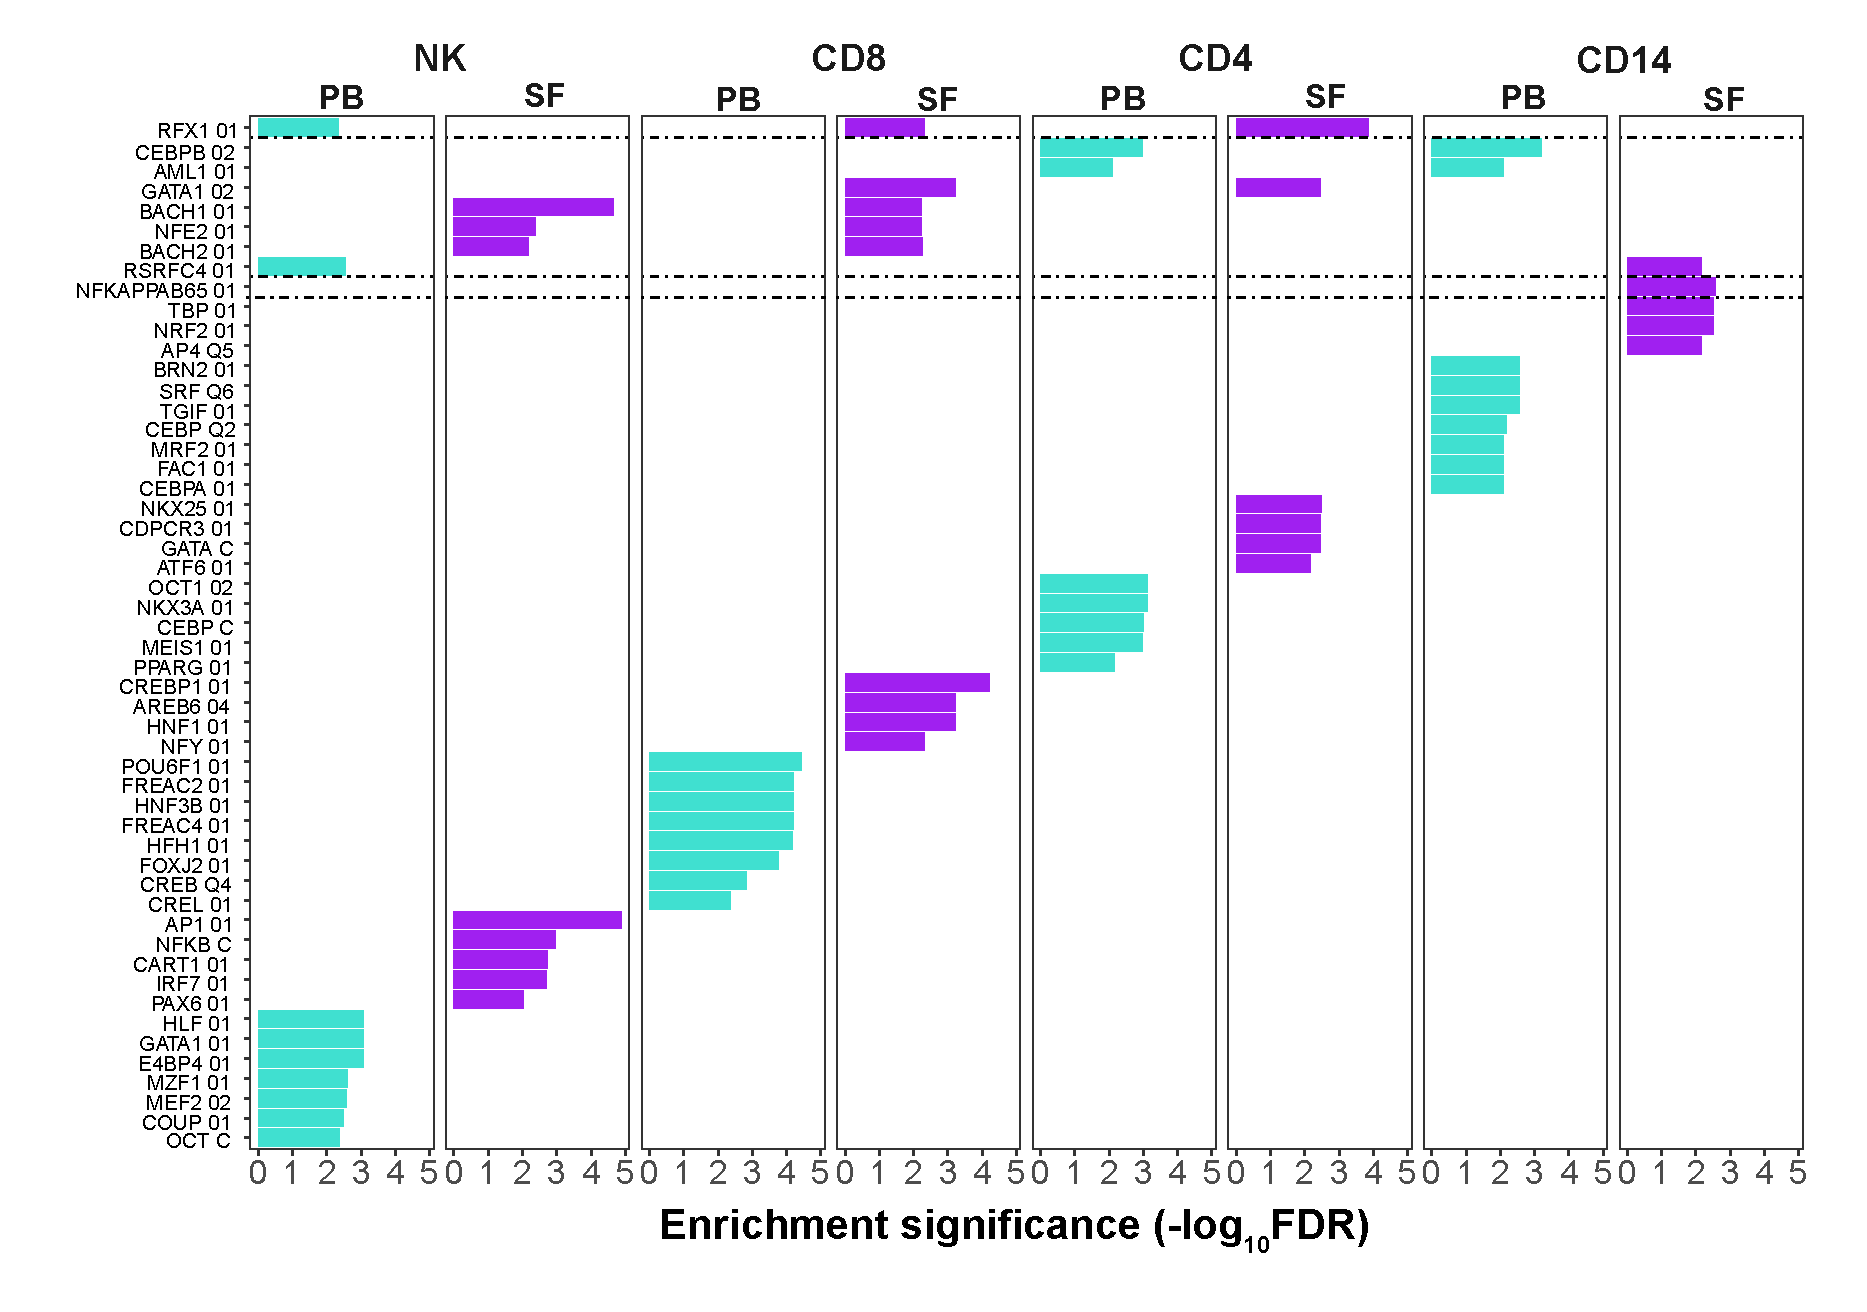
\includegraphics[width=0.8\textwidth]{./Results3/pdfs/ATAC_PSA_enrichment_conserved_TFBS_barplots_cell_type_specific_DOCS_all_cell_types_per_tissue}
%\caption[Enrichment of eRNA cell type-specific PsA DARs for conserved TFBS.]{\textbf{Enrichment of eRNA cell type-specific PsA DARs for conserved TFBS.} xxxx }
%\label{figure:PSA_TFBS}
%\end{figure}



\subsection{Differential gene expression analysis in paired circulating and synovial immune cells}

\subsubsection{Immune-relevant gene expression by qPCR}
%Introductory paragraph to link to ATAC-seq data
Mapping chromatin accessibility represents an informative tool to identify regulatory elements undergoing histone modifications, DNA methylation and TF binding, as previously explained. All those elements are involved in the regulation of gene expression, making the study of chromatin accessibility a good proxy for the inference of gene expression. Nevertheless, the characterisation of the chromatin landscape also presents some limitations, including the discordance between open chromatin and functionality of the regulatory element, shown by CAGE studies, as well as the identification of the target gene regulated by a particular element. 

In order to contextualise the ATAC-seq data, qPCR gene expression analysis for 370 key genes in the inflammatory and autoimmune response was conducted in CD14$^+$ monocytes, mCD4$^+$ and mCD8$^+$ cells isolated from SF and PB of three PsA patients (Table \ref{tab:PSA_datasets_per_sample}). Those appeared as the most abundant cell types in PB and SF from patients, and particularly mCD4$^+$ and mCD8$^+$ cells have been shown to expand in PsA inflammed synovium, as previously mentioned. The PCR array represented a cost-effective approach to study gene expression between PB and SF focusing in a relevant subset of genes of notably importance, given the inflammatory component in PsA. For each cell types, FC in expression was calculated pair-wise for SF respect to PB within each sample for each individual genes (detailed in Chapter \ref{ch:Mat}). Likely due to the small sample size,the majority of the modulated genes between SF and PB lacked of significance (FDR$<$0.05) after multiple testing correction. Therefore, to explore the biological relevance of this data, a less stringent pval$<$0.05 was used as the filtering threshold. 

% Since I am not used corrected pval Hai mentioned that I can not talk about differentially expressed
When considering the significantly modulated genes (pval$<$0.05) in at least one cell type, 
differences in magnitude and reproducibility in FCs were observed across samples and cell types (Figure \ref{figure:PSA_PCR_array_5pcnt_heatmap}). Some of the modulated genes showed up-regulation (FC$>$1.5) in SF compared to PB across the three cell types, for example \textit{FN1}, \textit{SPP1} or \textit{CCL2}, amongst others (Figure \ref{figure:PSA_PCR_array_5pcnt_heatmap} orange box). On the other hand, a number of genes presented reduced expression in SF (FC$<$1.5) in at least one of the three cell types, including \textit{FOS}, \textit{IL16}, \textit{PPBP} and \textit{TPST1} (Figure \ref{figure:PSA_PCR_array_5pcnt_heatmap} purple box). Also, a number of genes were only consistently modulated in the three CD14$^+$ monocyte samples but not in T cells (Figure \ref{figure:PSA_PCR_array_5pcnt_heatmap} dark blue box). 

\begin{landscape}
\begin{figure}[H]
\centering
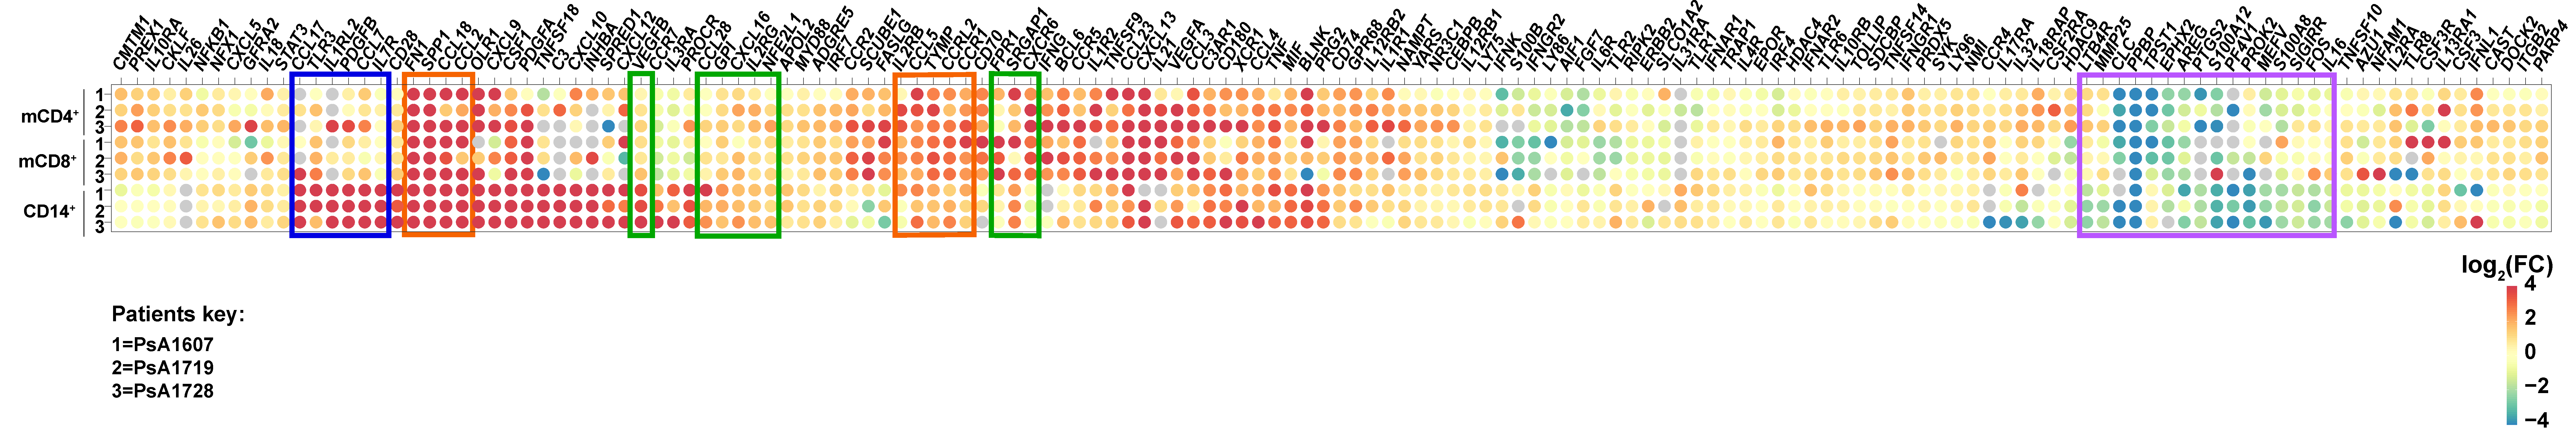
\includegraphics[width=1.5\textwidth]{./Results3/pdfs/PCR_array_PSA_SF_vs_PB_filtered_5_percent_genes_heatmap_New}
\caption[Heatmap of gene expression FCs between SF and PB for those gene significantly modulated (pval$<$0.05) in at least one cell type.]{\textbf{Heatmap of gene expression FCs between SF and PB for those gene significantly modulated (pval$<$0.05) in at least one cell type.} Amongst the 370 genes measured by qPCR, the FC in gene expression between the SF and PB for each pair of samples has been represented only those genes which were consistently modulated across the three PsA samples (pval$<$0.05) in at least one of the cell types. Each column represents a genes and each row a pair of SF-PB PsA samples. The log${_2}FC$ in gene expression between SF and PB is colour-coded. Overall, the heatmap allows to observe the change in gene expression as well as the magnitude between SF and PB for each gene in each of the the three pairs of PsA samples in CD14$^+$ monocytes, mCD4$^+$ and mCD8$^+$ cells.}
\label{figure:PSA_PCR_array_5pcnt_heatmap}
\end{figure}
\end{landscape}

For example, \textit{CCR7} and \textit{IL7R} were up-regulated in SF CD14$^+$ monocytes compared to PB; however changes between SF and PB were not consistent across patients in mCD4$^+$ and mCD8$^+$. Moreover, differences in the magnitude of FCs were also observed for some of the genes modulated in the same direction across the three cell types, for instance \textit{VEGFB} and \textit{CXCR6} (Figure \ref{figure:PSA_PCR_array_5pcnt_heatmap_New} green box).


Filtering of all the genes tested for expression in the qPCR array based statistical significance (pval$<$0.05) and mean FC$>$1.5 revealed CD14$^+$ monocytes and mCD8$^+$ presenting greater number of significantly modulated genes (72 and 77, respectively) compared to mCD4$^+$ cells (46 genes) (Figure \ref{figure:PSA_PCR_array_vulcano_plots} a, b and c). For the three analysed cell types, the majority of modulated immune genes showed up-regulation in the SF (Figure \ref{figure:PSA_PCR_array_vulcano_plots} a, b and c). For example, 56 out of the 70 significantly modulated genes in CD14$^+$ monocytes showed mean FC$>$1.5 versus the 14 genes with mean FC$<$1.5 (Figure \ref{figure:PSA_PCR_array_vulcano_plots} a).



% May need a bit more of biology there
\begin{figure}[htbp]
\centering
\begin{subfigure}{0.5\textwidth}
\centering
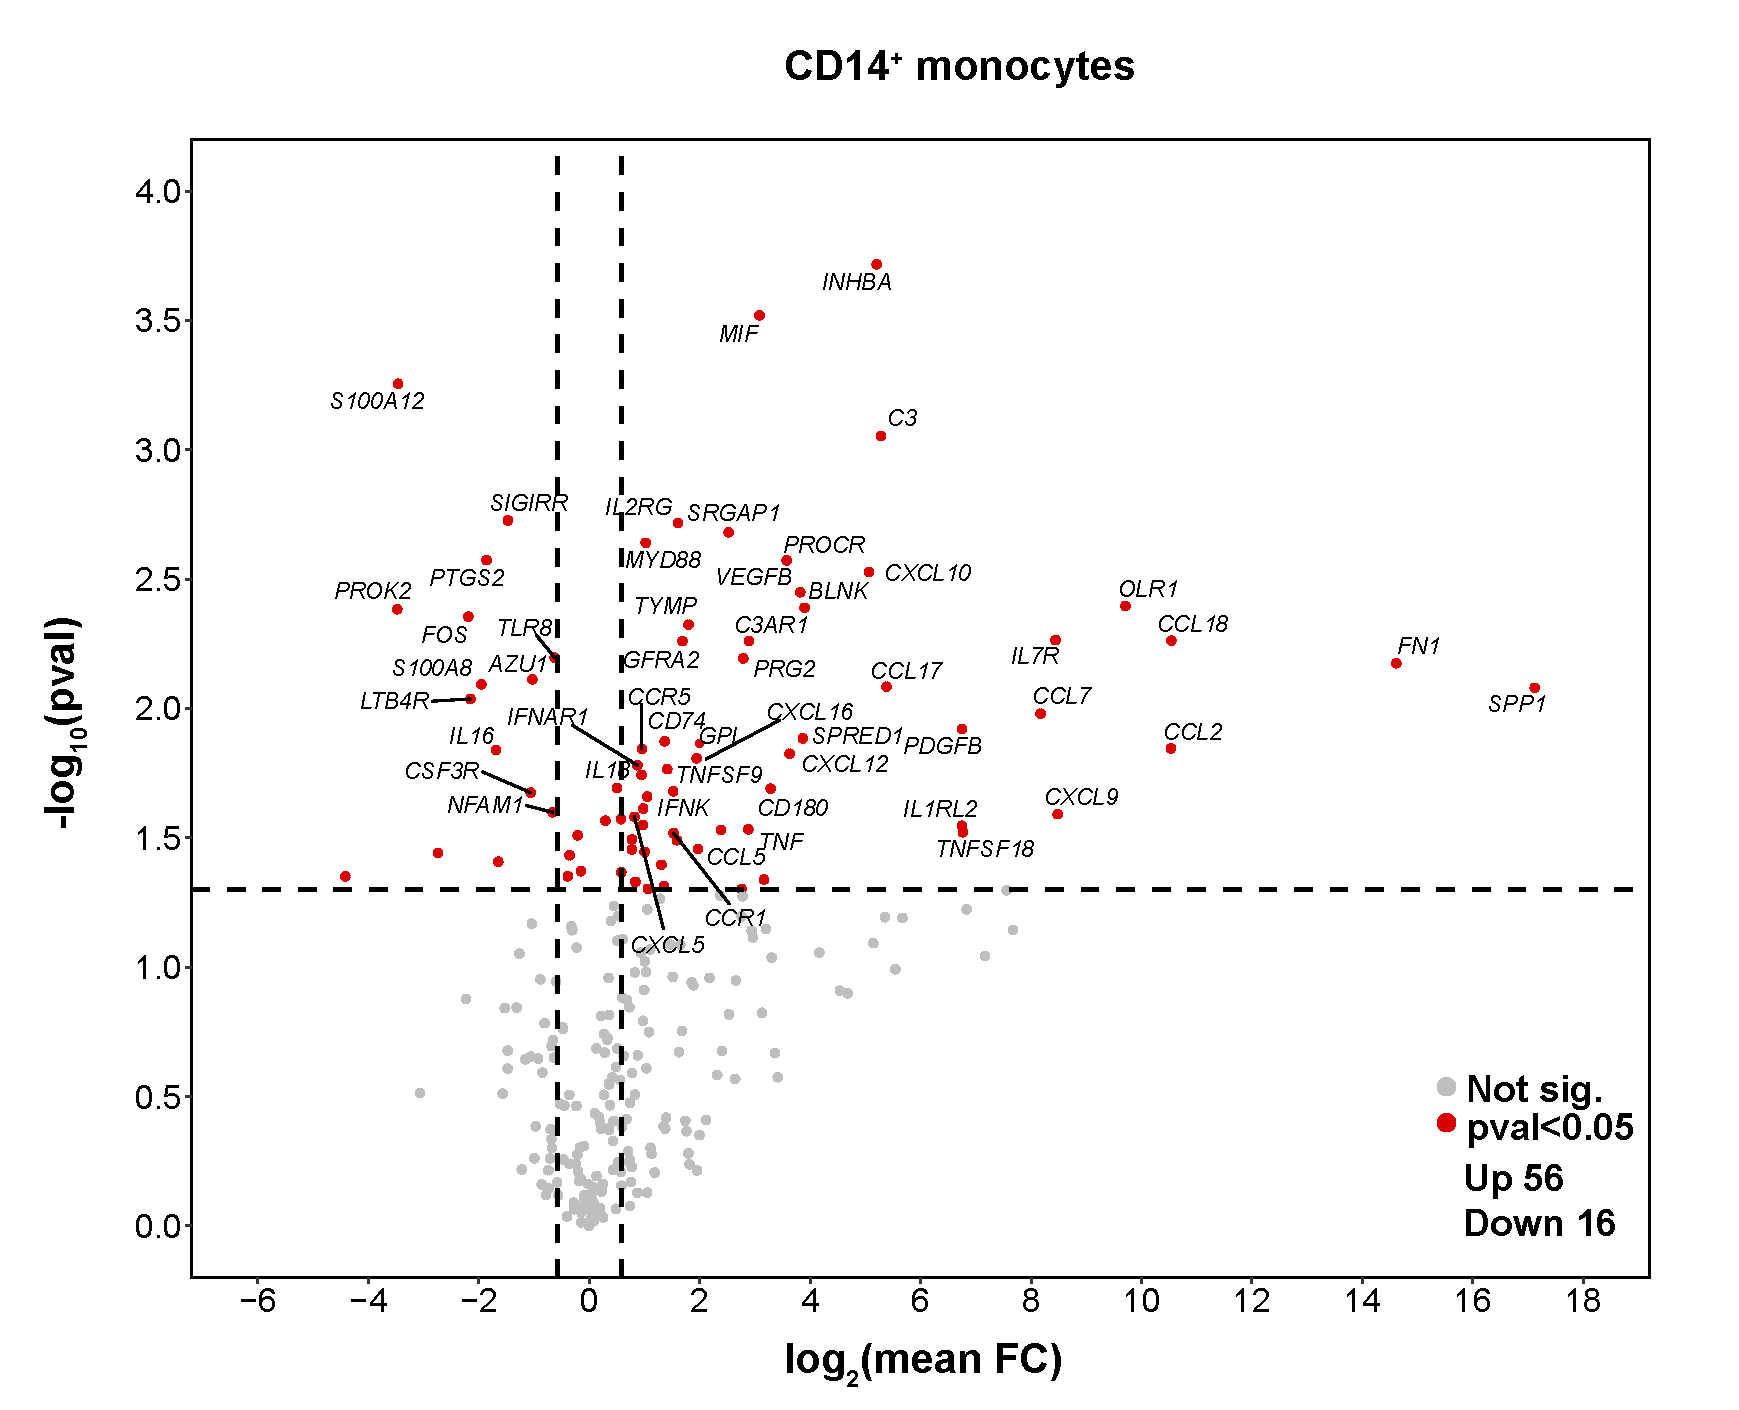
\includegraphics[width=\textwidth]{./Results3/pdfs/PSA_CD14_vulcano_plot_PCR_array_mean_FC}
\caption{\textbf{}}
% The percentage sign indicated that the other subfig goes side by side
\end{subfigure} \\
\begin{subfigure}{0.5\textwidth}
\centering
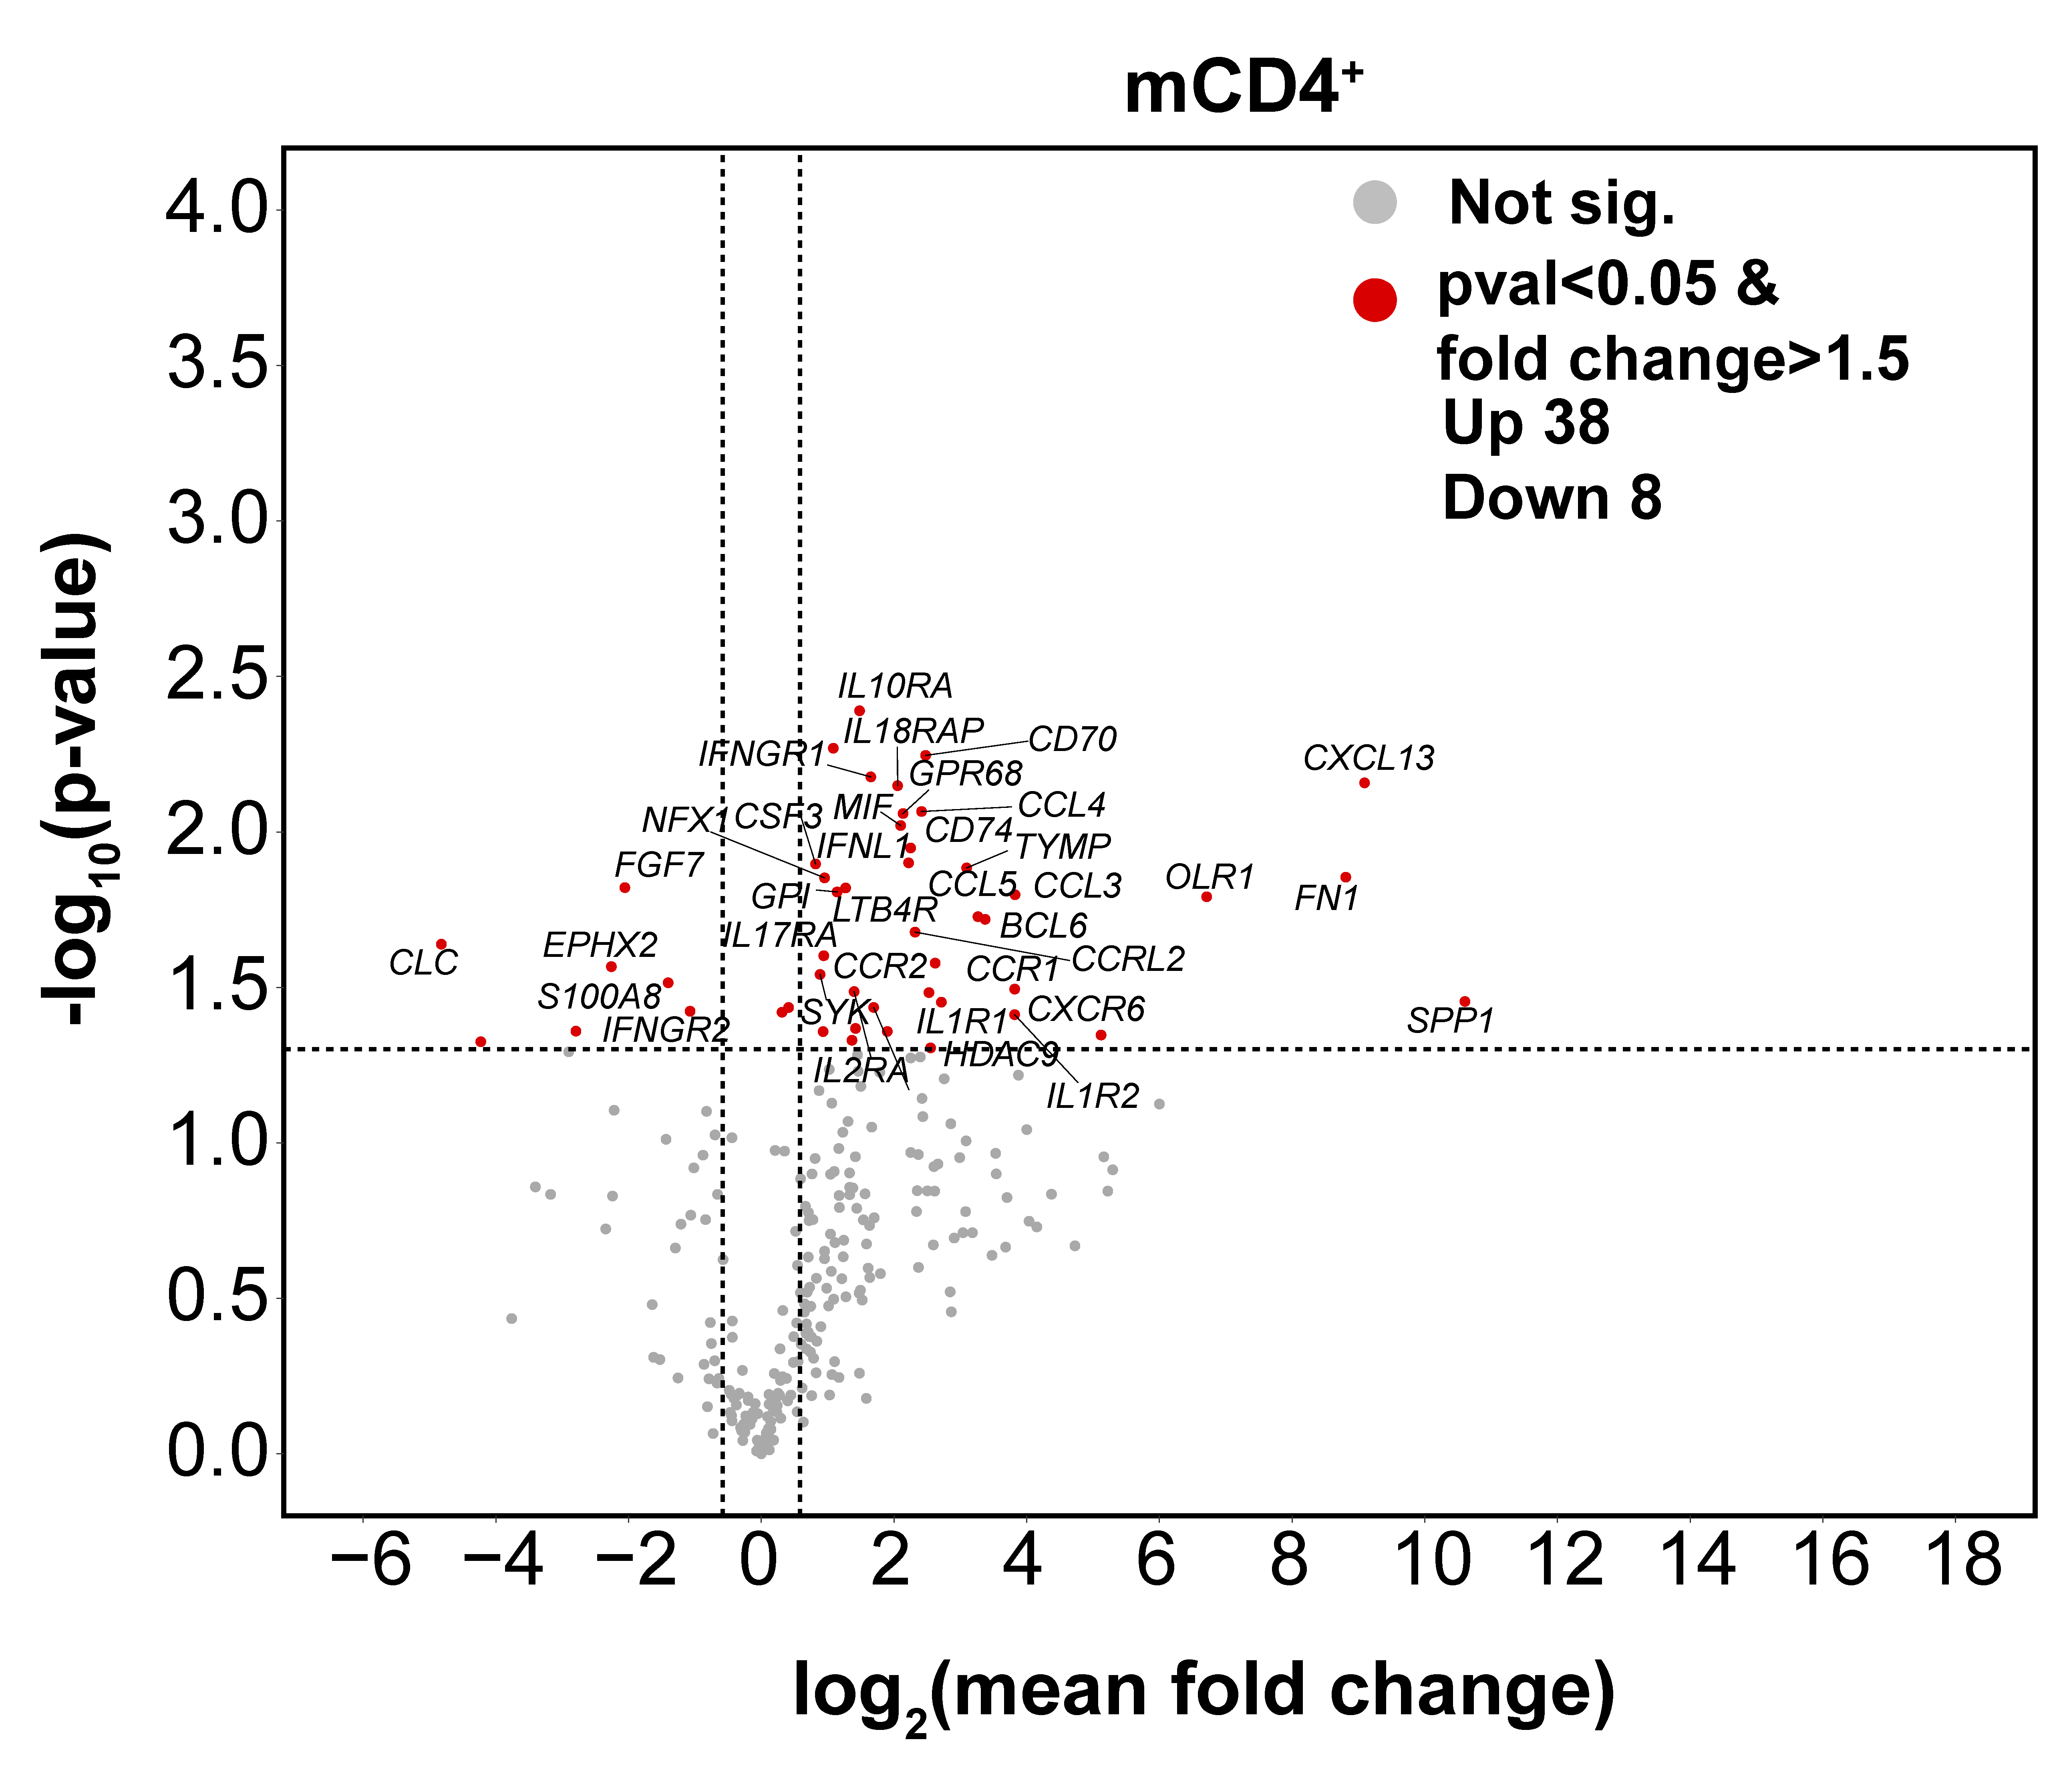
\includegraphics[width=\textwidth]{./Results3/pdfs/PSA_CD4_vulcano_plot_PCR_array_mean_FC}
\caption{\textbf{}}
\end{subfigure} %
\begin{subfigure}{0.5\textwidth}
\centering
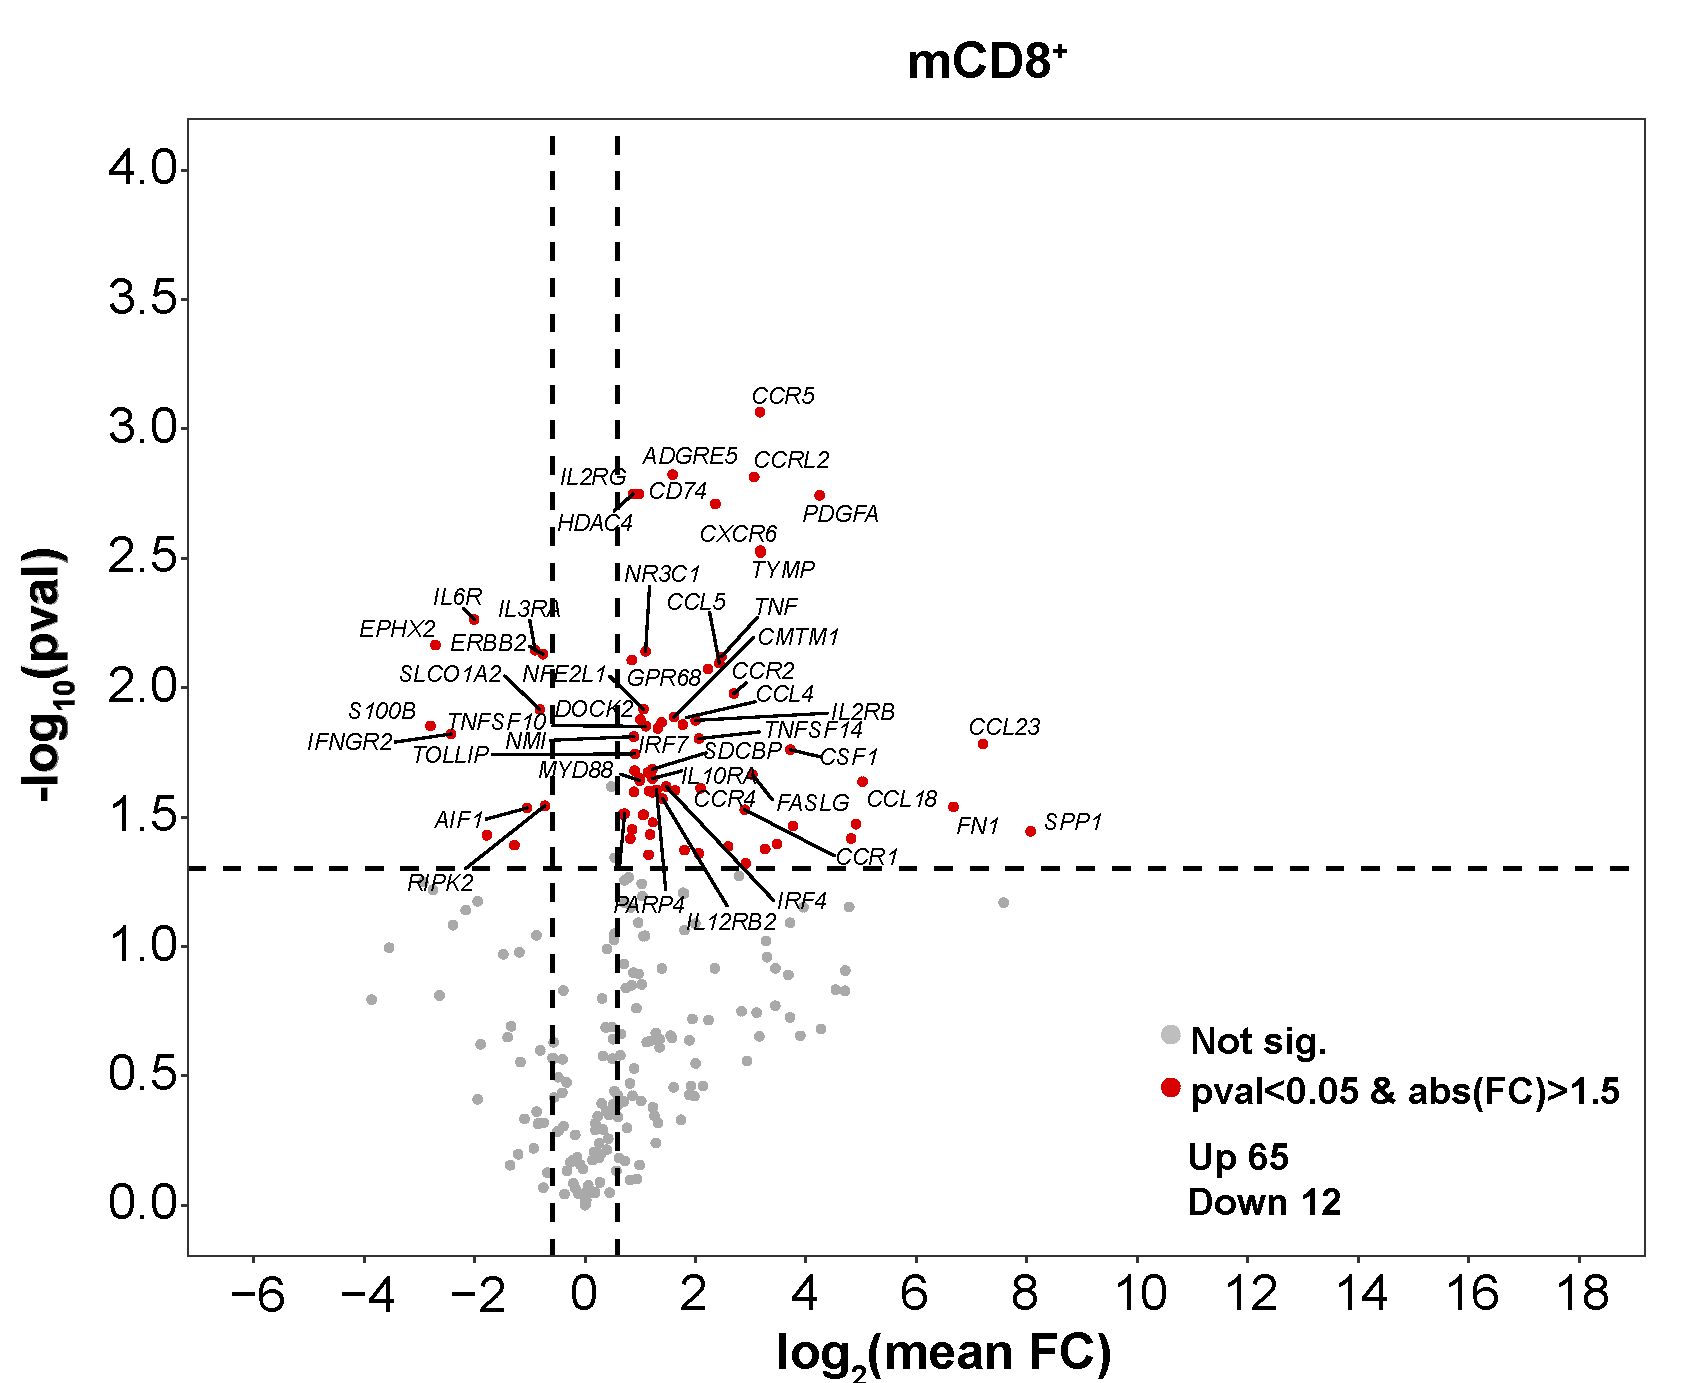
\includegraphics[width=\textwidth]{./Results3/pdfs/PSA_CD8_vulcano_plot_PCR_array_mean_FC}
\caption{\textbf{}}
\end{subfigure}
\caption[Gene expression changes in immune-relevant genes between SF and PB in CD14$^+$ monocytes, mCD4$^+$ and mCD8$^+$ cells.]{\textbf{Gene expression changes in immune-relevant genes between SF and PB in CD14$^+$ monocytes, mCD4$^+$ and mCD4$^+$ cells.} Vulcano plots showing differences in gene expression measured by qPCR array between SF and PB for a) CD14$^+$ monocytes, b) mCD4$^+$ and c) mCD8$^+$ cells. The significance (log${_10}$pval) of the modulation in gene expression between the two tissues (y-axis) is plotted against the log${_2}$ of the mean FC across the three PsA patients. Positive FC indicates higher expression in SF. Genes showing pval$<$0.05 and mean FC$>$1.5 are coloured in red, with the most significant genes labelled.}
\label{figure:PSA_PCR_array_vulcano_plots}
\end{figure} 




\subsubsection{Correlation between gene expression and chromatin accessibility}
% ATAC overall overlap
Overlap between differentially modulated genes and DARs in the proximity were observed in the three cell types (Table \ref{tab:PSA_gene_expression_ATAC_overlap}). The overlap in CD14$^+$ monocytes revealed significant enrichment of modulated genes between SF and PB for DARs with the same direction of change (Fisher exact test pval=0.028). In contrast to CD14$^+$ monocytes, the observed overlap between gene expression and chromatin accessibility did not appear to be significant in mCD4$^+$ and mCD8$^+$ cells (Fisher exact test pval=0.466 and 0.173, respectively).


\begin{table}[htbp]
%\setlength{\tabcolsep}{20pt} only to stretch the columns if you want
%\renewcommand{\arraystretch}{1.5}
\centering
\begin{tabular}{@{} c c c}
\toprule
\textbf{Cell type} & \textbf{Genes up-regulated and}        &  \textbf{Genes down-regulated and} \\
                   & \textbf{overlapping open chromatin}   &  \textbf{overlapping closed chromatin} \\
									 &	\textbf{in SF}				               &  \textbf{in SF} \\
\midrule
\midrule
          & 13 (\textit{BLNK}, \textit{CCL2$^\ast$}, \textit{CCR1$^\ast$}, \textit{CD180}, & 2 (\textit{FOS}, \textit{PROK2$^\ast$}) \\      CD14$^+$  & \textit{CXCL10}, \textit{FN1}, \textit{IL18}, \textit{IL31RA$^\ast$},    & \\
monocytes & \textit{IL7R$^\ast$}, \textit{NFKB1$^\ast$}, \textit{PRG2}, \textit{SRGAP1}, & \\
				  & \textit{STAT3}) & \\
				
\midrule
mCD4$^+$ & 3 (\textit{CXCL13}, \textit{CXCR6$^\ast$}, \textit{IL2RA}) & 0 \\

\midrule
mCD8$^+$ & 6 (\textit{CCL3}, \textit{CCR2}, \textit{CCR5} ,\textit{IRF4} & 1 (\textit{EPHX2}) \\
         & \textit{TNFSF10}, \textit{YARS}) & \\

\bottomrule
\end{tabular}
\medskip %gap
\caption[Immune genes with significant modulated expression in SF and proximal to a DAR in Fast-ATAC.]{\textbf{Immune genes with significant modulated expression in SF and proximal to a DAR in Fast-ATAC.} An overlap is defined by significant change in expression (pval$<$0.05) of a particular gene where there is also a proximal DAR showing changes in chromatin accessibility in the same direction. ($^\ast$) indicates that the proximal DAR overlapping an eRNA identified by FANTOM5 project in that particular cell type (see subsection Characterisation of the differential accessible chromatin regions).}
\label{tab:PSA_gene_expression_ATAC_overlap}
\end{table}

In CD14$^+$ monocytes, 13 out of the 56 significantly up-regulated genes in SF overlapped with SF open DARs. For example, the increased expression of \textit{IL7R} in SF correlated with increased chromatin accessibility at the 5' and 3' UTR of this gene, previously shown (Figure \ref{figure:PsA_FAST_ATAC_gene_boy_DOCS_CD14_NK} b). Another relevant example was the \textit{FN1} gene, which up-regulated expression in synovial biopsies compared to PB has already been reported by others \parencite{Dolcino2015}. In this cohort, \textit{FN1} expression was up-regulated in SF for all three cell types with the greater FC found in CD14$^+$ monocytes (Figure \ref{figure:PSA_PCR_array_vulcano_plots} a), concomitantly with more accessible chromatin at the promoter and downstream the 3' UTR of the gene (Figure \ref{figure:PSA_CD14_ATAC_FN1}). Lesser overlap between up-regulated gene expression and open chromatin in SF compared to PB was observed in mCD4$^+$ and mCD8$^+$ (6 and 3 hits, respectively). Only CD14$^+$ monocytes and mCD8$^+$ cells presented overlap between SF down-regulated genes and proximal less accessible in SF (2 and 1, respectively). Notably, none or very few genes presented opposite direction of change in gene expression and chromatin accessibility on a proximal DAR (4 in CD14$^+$ monocytes, 0 in mCD4$^+$ and 2 in mCD8$^+$), reinforcing the biological relevance of the observed overlaps. 
%decide which example to use: I have included IL7R in monocytes and maybe could use FN1 to complete
	%Example expression in CD14 FOS,FN1,CCL2,CXCL10
	
\begin{figure}[htbp]
\centering
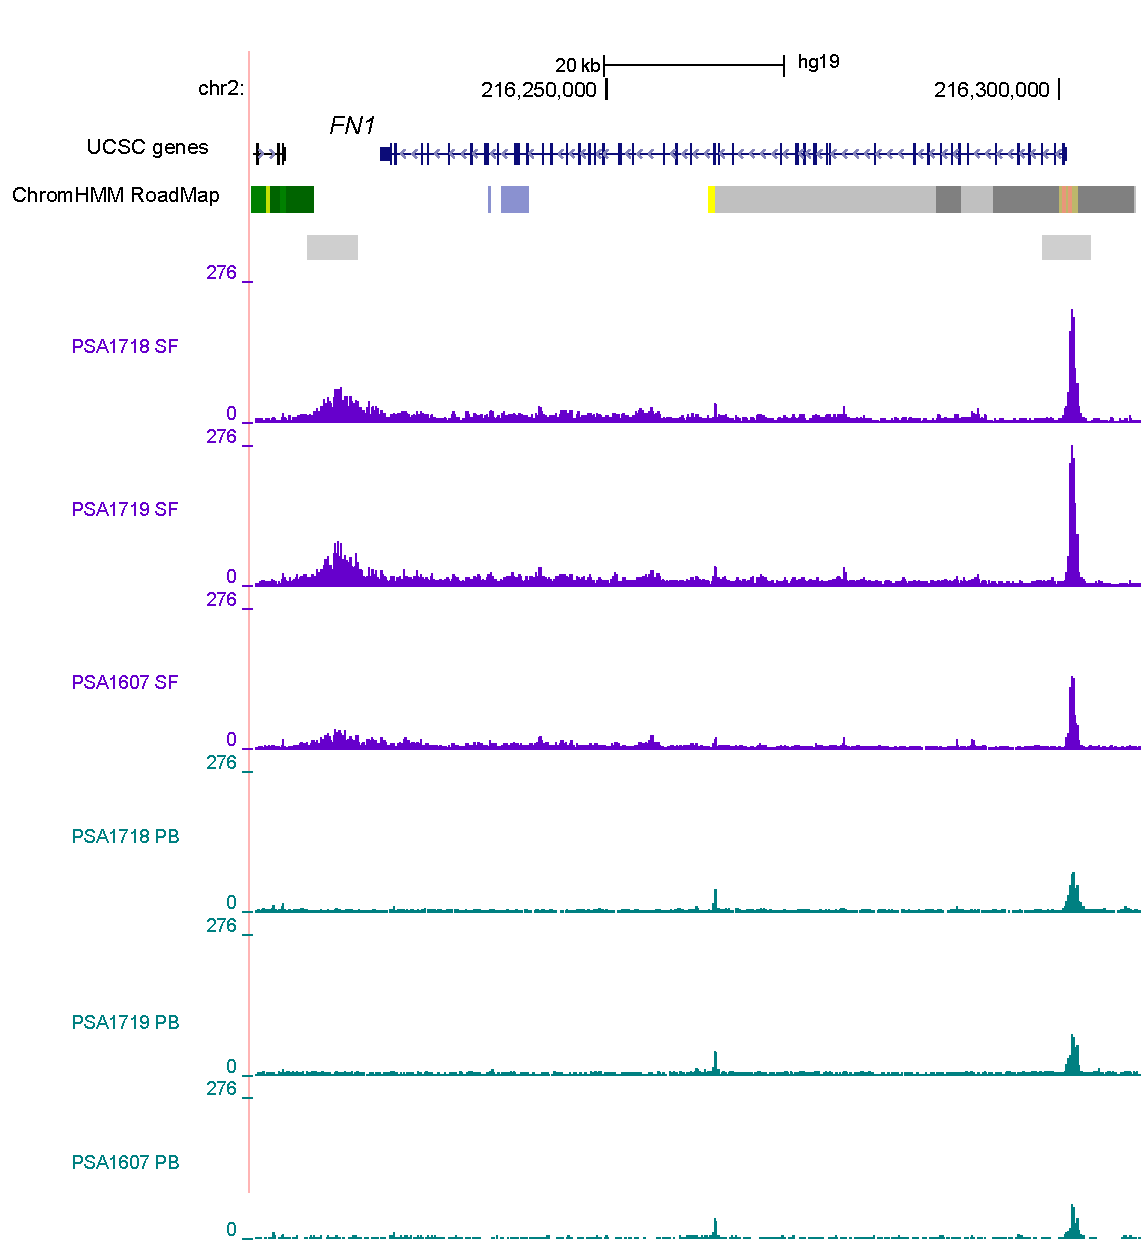
\includegraphics[width=0.6\textwidth]{./Results3/pdfs/PSA_CD14_ATAC_FN1_paired_gene_expression}
\caption[Chromatin accessibility landscape at the qPCR differentially expressed \textit{FN1} gene in CD14$^+$ monocytes.]{\textbf{Chromatin accessibility landscape at the qPCR differentially expressed \textit{FN1} gene in CD14$^+$ monocytes.} UCSC Genome Browser view illustrating the ATAC normalised read density (y-axis) in two DARs located at the promoter and downstream the 3' UTR of the \textit{FN1} gene (x-axis) in CD14$^+$ monocytes from SF and PB in three PsA patients. Both DARs were more accessible in SF when compared to PB. Tracks are colour-coded by tissue (SF=purple and PB=turquoise). The Epigenome Roadmap chromatin segmentation track for PB isolated CD14$^+$ monocytes is also shown. All DARs were significant based on FDR$<$0.01 and FC$>$1.5.}
\label{figure:PSA_CD14_ATAC_FN1}
\end{figure}


\subsubsection{Pathway enrichment and network analysis highlights the role of synovial CD14$^+$ monocytes in cytokine and chemokine production}
%Describe pathway analysis results and curate the pathway of interest
To identify relevant pathways amongst the modulated genes between SF and PB, enrichment analysis was performed for each individual cell type. Up-regulated and down-regulated genes showing abs mean FC$>$1.5 and pval$<$0.05 were used as input for the enrichment analysis. Interestingly, the modulated genes between SF and PB in CD14$^+$ monocytes were enriched for chemokine, NOD-like signalling and TLR signalling pathways (Table \ref{table:PSA_PCR_array_pathway_analysis}). All three pathways are involved in the activation of cytokines and chemokines gene expression, leading to T cell recruitment and inflammatory response. 

The TLR signalling pathways enrichment involved the \textit{FN1} (previously mentioned) and \textit{SPP1}, two of the top differentially expressed genes found in this pilot study (Table \ref{table:PSA_PCR_array_pathway_analysis}). Together with \textit{FN1}, \textit{SPP1} was highly up-regulated (mean FC$>$16) in the three cell types, showing the greatest FC in monocytes (Figure \ref{figure:PSA_PCR_array_vulcano_plots} a). Moreover, some of the genes driving enrichment, such as \textit{CCL5} and \textit{NFKB}, were also shared across the three pathways of interest. Others genes, including \textit{TNF}, \textit{IRF7} and \textit{MYD88}, highlighted the cross-link between the NOD-like and the TLR signalling pathways. 

Accordingly, the enrichment of SF open DARs in CD14$^+$ monocytes for the NF$\kappa$B pathway is closely related to the enrichment for TLR and NOD-like signalling pathways at the transcriptomic level, since both pathways lead to the activation of the NF$\kappa$B TF  (Figure \ref{figure:PSA_ATAC_pathway_analysis_all_DOC} a). %Both, TLR and NOD-like pathways lead to the activation of the NF$\kappa$B TF, which induces transcriptional activation of pro-inflammatory cytokines, further supported by the enrichment of SF open DARs in the proximity of genes from the IL-2, IL-3, IL-5 and GM-CSF pathways (Figure \ref{figure:PSA_ATAC_pathway_analysis_all_DOC} a). Moreover, the pivotal role of NF$\kappa$B in the immune transcriptional profile of SF CD14$^+$ monocytes is additionally sustained at the chromatin accessibility level by the enrichment of SF accessible chromatin sites for this TF (Figure \ref{figure:PSA_TFBS}).  

The enrichment for the chemokine pathway in CD14$^+$ monocytes (Table \ref{table:PSA_PCR_array_pathway_analysis}) included modulated genes highly up-regulated (mean FC$>$16) in SF compared to PB (e.g \textit{CCL18} and \textit{CCL2}) for all three cell types (Figure \ref{figure:PSA_PCR_array_vulcano_plots}) as well as genes only consistently modulated between SF and PB in CD14$^+$ monocytes (e.g \textit{CCL28}, Figure \ref{figure:PSA_PCR_array_5pcnt_heatmap} green box). %The chemokine pathway includes production of chemotractant molecules involved in the recruitment of leukocytes to the site of inflammation and reactive oxygen species (ROS) through Ca$^2$$^+$ mobilisation, a pathway that has previously presented to be enriched in SF open DARs in CD14$^+$ monocytes (Figure \ref{figure:PSA_ATAC_pathway_analysis_all_DOC} a).

At the transcriptional level, significantly modulated genes between SF and PB in mCD4$^+$ T cells were enriched for the IL-10 signalling pathway (Table \ref{table:PSA_PCR_array_pathway_analysis}), in lines with the enrichment for IL signalling of open chromatin in SF cells (Figure \ref{figure:PSA_ATAC_pathway_analysis_all_DOC} b). % Add reference to this pathway in disease


\begin{landscape}
\begin{center}
\begin{longtable}[ht]{c c c }
\caption[Pathway enrichment analysis for the modulated genes between SF and PB in CD14$^+$ and mCD4$^+$.]{\textbf{Pathway enrichment analysis for the modulated genes between SF and PB in CD14$^+$ and mCD4$^+$.} The analysis was performed using only those genes showing pval$<$0.05 and mean FC$>$1.5. Reported enriched pathways were significant at an FDR $<$0.05.}
\label{table:PSA_PCR_array_pathway_analysis} \\
\toprule
\textbf{Cell type} & \textbf{Pathway} & \textbf{Genes} \\						
\midrule
\midrule
\textbf{CD14$^+$} & Chemokine signalling & \textit{CCL17}, \textit{CCL18}, \textit{CCL2}, \textit{CCL28}, \textit{CCL5}, \textit{CCL7}, \textit{CCR1}, \textit{CCR5},\textit{CXCL10} \\  
									&                             & \textit{CXCL12}, \textit{CXCL16}, \textit{CXCL5}, \textit{CXCL9}, \textit{NFKB1}, \textit{PPBP}, \textit{PF4V1}, \textit{STAT3}, \textit{XCR1}\\
									
									& NOD-like receptor signalling & \textit{CCL2}, \textit{CCL5}, \textit{IFNAR1}, \textit{IL18}, \textit{IRF7}, \textit{MEFV}, \textit{MYD88}, \textit{NFKB1}, \\
									&                                         & \textit{NAMPT}, \textit{TNF} \\

									& TLR signalling   & \textit{CCL5}, \textit{CXCL10}, \textit{CXCL9}, \textit{IFNAR1}, \textit{IRF7}, \textit{MYD88}, \textit{NFKB1}, \textit{SPP1},\textit{FOS},\\ 
									&                                         & \textit{TLR1}, \textit{TLR2}, \textit{TLR8}, \textit{TNF}\\

\midrule
\textbf{mCD4$^+$} & IL-10 signaling & \textit{CCL3}, \textit{CCL4}, \textit{CCL5}, \textit{CCR1}, \textit{CCR2}, \textit{CSF1}, \textit{CSF3}, \textit{IL10RA}, \\
									&									& \textit{IL1R1}, \textit{IL1R2}\\
\bottomrule
\medskip
\end{longtable}
\end{center}
\end{landscape}

In addition to pathway enrichment, network analysis was performed to understand the interaction and relationship of the genes with modulated expression between SF and PB. A gene subnetwork was identified from the STRING functional interaction database using as input all the genes from the qPCR array (regardless pval significance and FC) and ranking them based on the best pval across the three analysed cell types. The identified subnetwork predominantly included significant modulated genes between SF and PB in at least one of the cell types. Amongst the most interesting nodes was the single Ig and Toll-interleukine domain containing gene (\textit{SIGIRR}), which is a negative regulator of the TLR signalling pathway (Figure \ref{figure:PSA_PCR_network_analysis}). \textit{SIGIRR} was significantly down-regulated in SF CD14$^+$ monocytes only and it is consistent with the significant up-regulation (pval<0.05) of the \textit{TLR1}, \textit{TLR2}, \textit{MYD88} genes in SF as well as the enrichment for the TLR pathway in this cell type (Figure \ref{figure:PSA_PCR_array_5pcnt_heatmap} and \ref{table:PSA_PCR_array_pathway_analysis}). Moreover, the significant up-regulation of \textit{NFKB} and \textit{TNF} in the SF CD14$^+$ monocytes appeared as a downstream result of the functional connection with TLR pathway members such as \textit{MyD88}, previously mentioned . Conversely, in mCD4$^+$ and mCD8$^+$ the modulation of these members did not appear to be significant between SF and PB.% however, in mCD8$^+$, \textit{TNF} expression is also significantly up-regulated in the synovium compared to PB. 

Another interesting part of the network is the connection of the TLR pathway and the chemokine production through \textit{NF$\kappa$B}, \textit{TNF} and \textit{CCL2} (Figure \ref{figure:PSA_PCR_network_analysis}). \textit{CCL2} is connected to \textit{CXCL10} and subsequently with \textit{CCL18} and \textit{CCR5}, all chemokines and chemokine receptors regulating migration and infiltration of monocytes and memory T cells at the sites of inflammation. This network analysis also highlighted relationship between \textit{IL7R} and \textit{IL2RG} coding for the two chains of the IL-7R. %Interestingly, these two nodes were only significantly up-regulated in SF CD14$^+$ monocytes when compared to PB, supporting the novel cell and context specific role of IL-7R and IL-7R polymorphism under inflammatory conditions in CD14$^+$ monocytes\parencite{Al-Mossawi2018}.

% I could also talk about the FOS, PROK2 and PTGS2

\begin{figure}[htbp]
\centering
\includegraphics[width=\textwidth]{./Results3/pdfs/PSA_PCR_array_network_analysis}
\caption[Protein network analysis based on the immune qPCR array expression data.]{\textbf{Protein network analysis based on the immune qPCR array expression data.} The list of all the genes quantified in the qPCR array genes together with the best pval for significance of the mean FC across the three cell types was used to perform gene network analysis. STRING interaction network (including known and predicted protein–protein interactions) was used to superpose the aforementioned list of genes and obtain a 30 gene size subnetwork common for all three cell types. This included maximal number of significant genes (pval$<$0.05) in at least one cell type and minimal presence of non-significant genes as linkers in the network. In the left hand panel, for each cell type each of the nodes (proteins) of the identified subnetwork (the same for each cell type, as previously explained) are colour-coded by the change of expression (log${_2}$ mean FC) for the corresponding gene in the qPCR analysis. On the right hand panel, each of the nodes in the same subnetwork are colour-coded by the level of significance (pval) for the reported modulation in gene expression (log${_2}$ mean FC) in the qPCR array.}
\label{figure:PSA_PCR_network_analysis}
\end{figure}



Overall, the integration of the chromatin accessibility and immune transcriptional data reinforced a relevant role of synovial CD14$^+$ monocytes in the production of cytokines and chemokines, likely leading to activation of the innate immune response and the recruitment of T cells to this site of inflammation. 



\subsubsection{Tissue and disease specificity in gene expression modulation and relevant biological pathways}

In order to better understand the disease and tissue specificity of the prior transcriptomic results, gene expression was analysed in CD14$^+$ monocytes, mCD4$^+$ and mCD8$^+$ isolated from PB in three healthy controls using the same qPCR array. In each of the cell types, the FC in was calculated for the mean PB expression across the three PsA patients compared to the mean expression of the three healthy controls (as detailed in Chapter \ref{ch:Mat}). Similar to the previous analysis, pvals for the FC significance were calculated for each particular genes. Integration of the previous results of modulated gene expression between SF and PB in PsA (see Immune-relevant gene expression by qPCR) with this analysis allowed the identification of three group of genes (Figure \ref{figure:PSA_PCR_array_HC_FC_correlation}). First, the genes only significantly modulated (based on pval and FC threshold criteria) in PB between controls and PsA were designated as systemic genes (Figure \ref{figure:PSA_PCR_array_HC_FC_correlation} green dots). Those genes were not significantly modulated in the prior analysis comparing SF versus PB within PsA patients and could then be considered as the circulating disease "footprint". In this respect, CD14$^+$ monocytes was the cell type with lower number of systemic modulated genes (14), compared to mCD8$^+$ (23) and mCD4$^+$ (42) (Figure \ref{figure:PSA_PCR_array_HC_FC_correlation}a, b and c). Amongst these genes were \textit{CCL24} and \textit{CCL27} in CD14$^+$ monocytes, \textit{CCR7} and \textit{TLR4} in mCD4$^+$ cells and \textit{CCR10} in mCD8$^+$ cells.  


\begin{figure}[htbp]
\centering
\begin{subfigure}{0.45\textwidth}
\centering
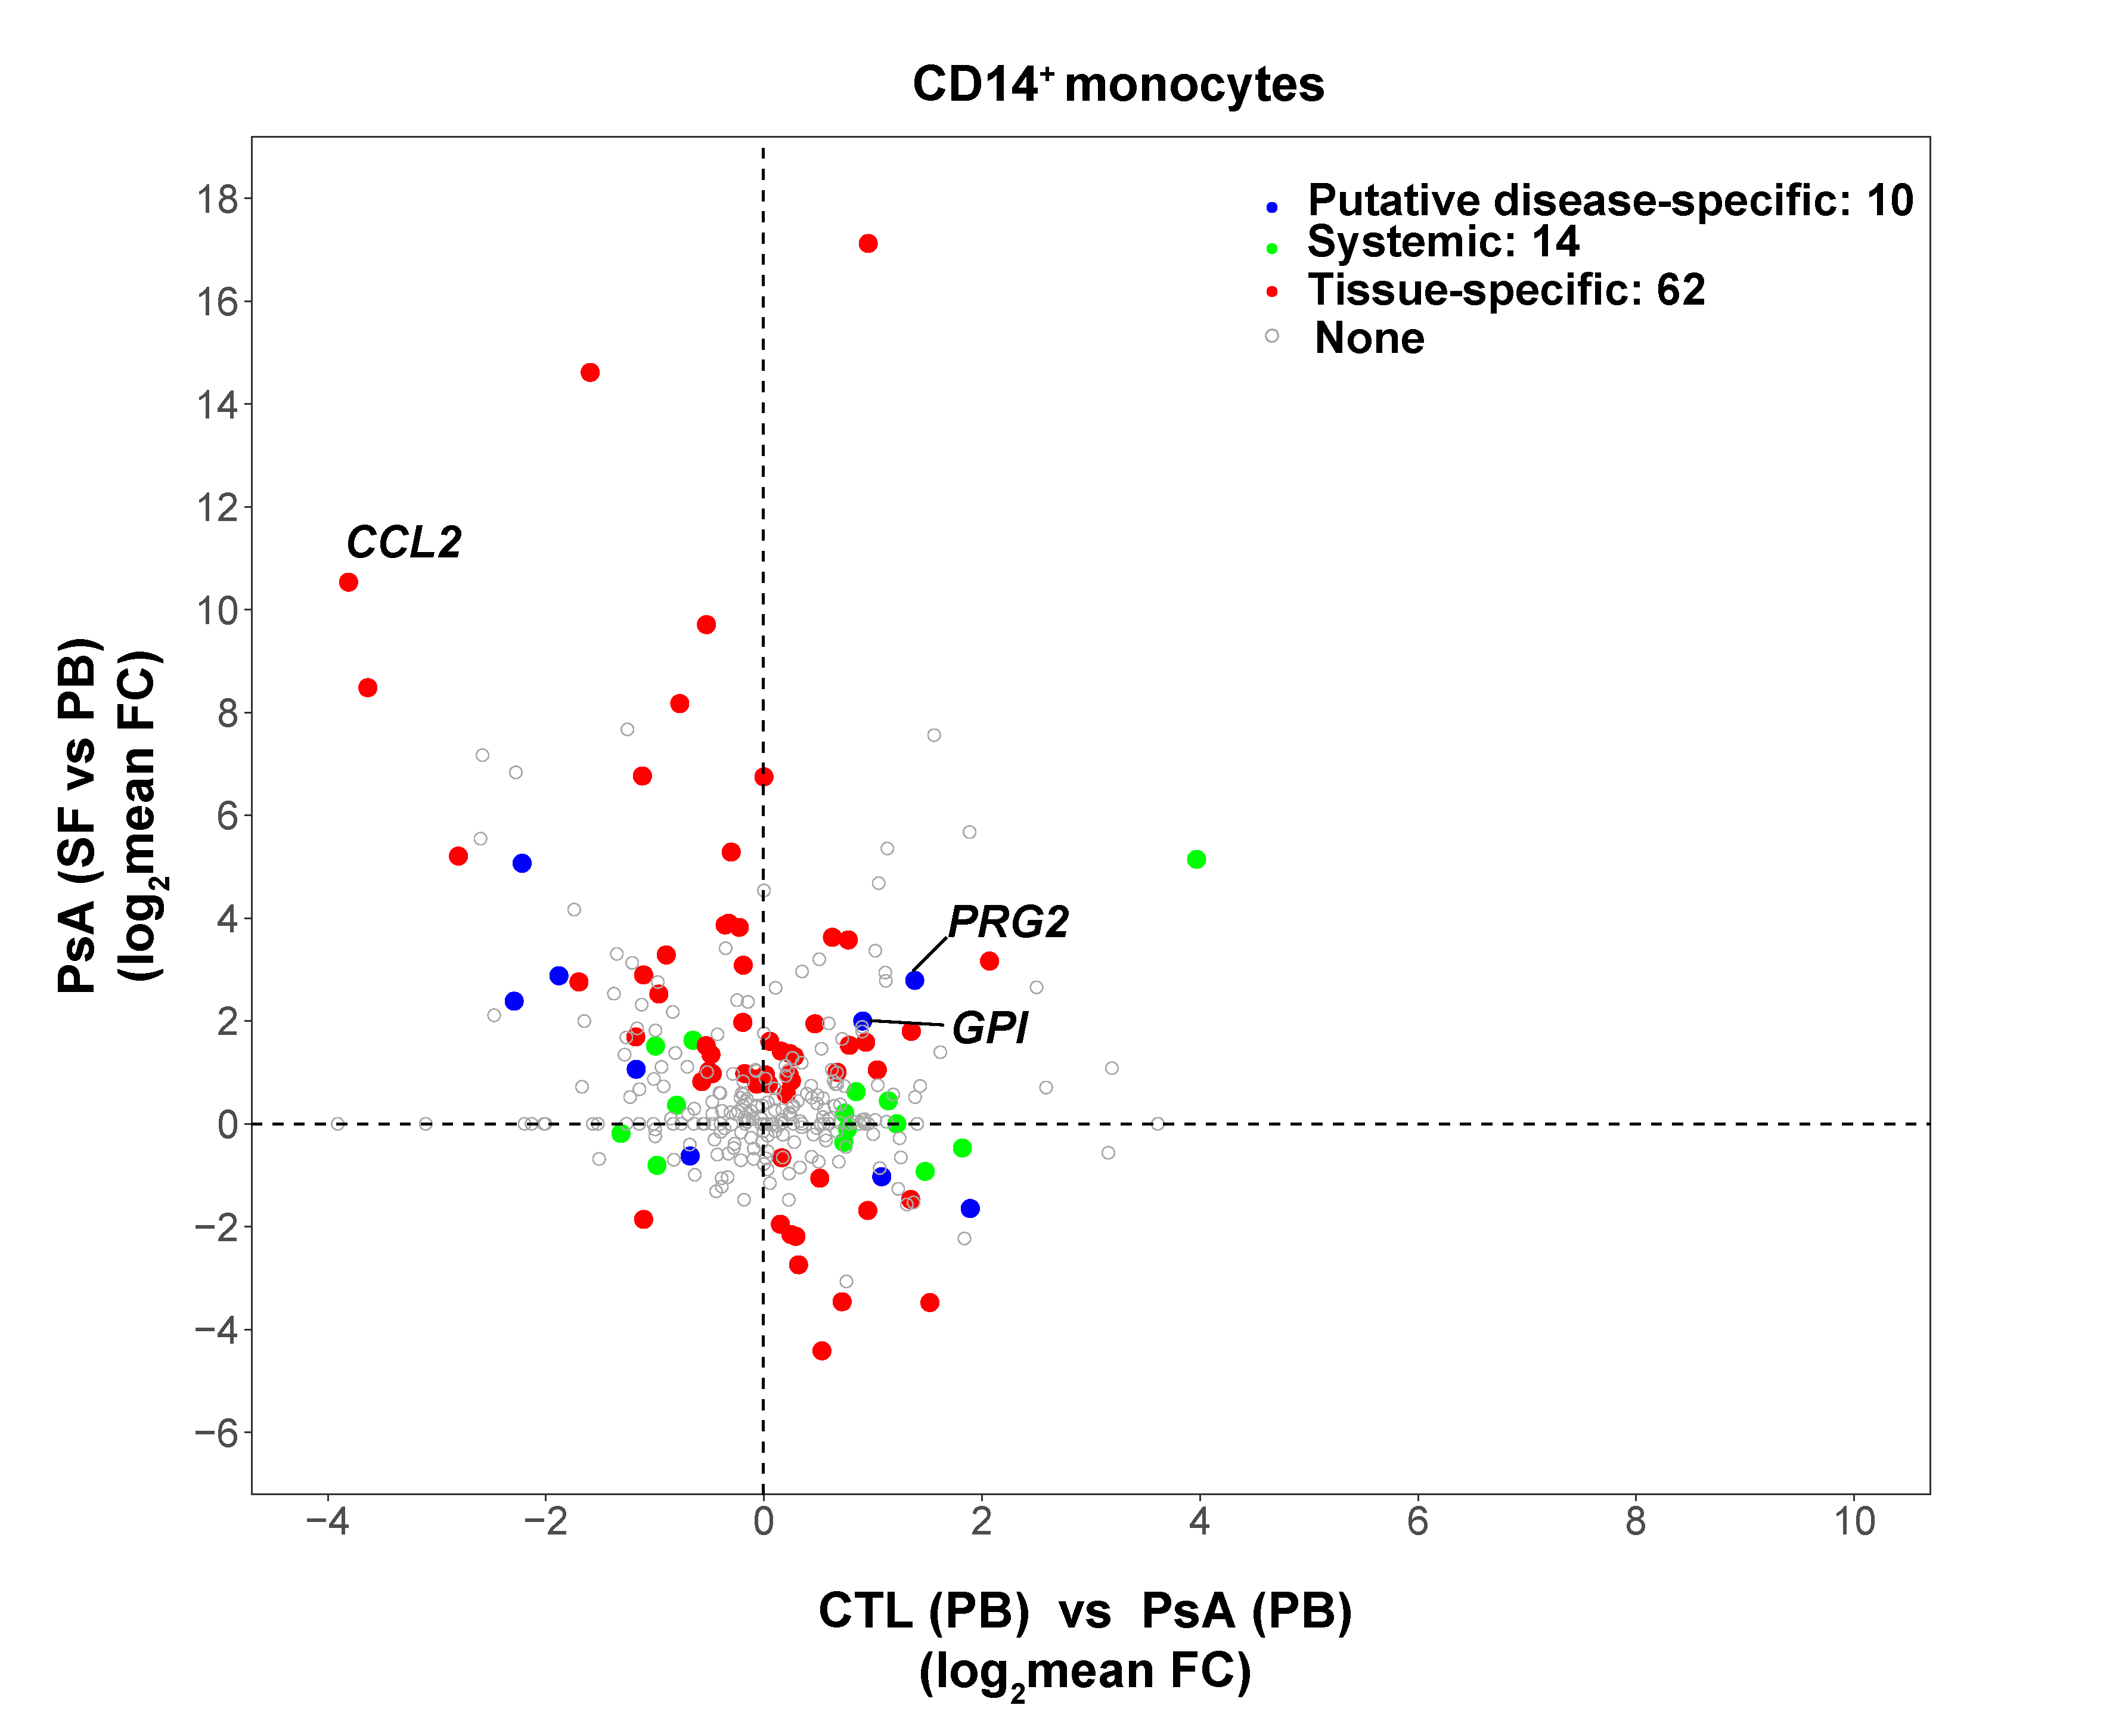
\includegraphics[width=\textwidth]{./Results3/pdfs/PSA_array_correlation_CD14_FC_HVPsA_vs_SFPBPsA_t}
\caption{\textbf{}}
% The percentage sign indicated that the other subfig goes side by side
\end{subfigure} \\
\begin{subfigure}{0.45\textwidth}
\centering
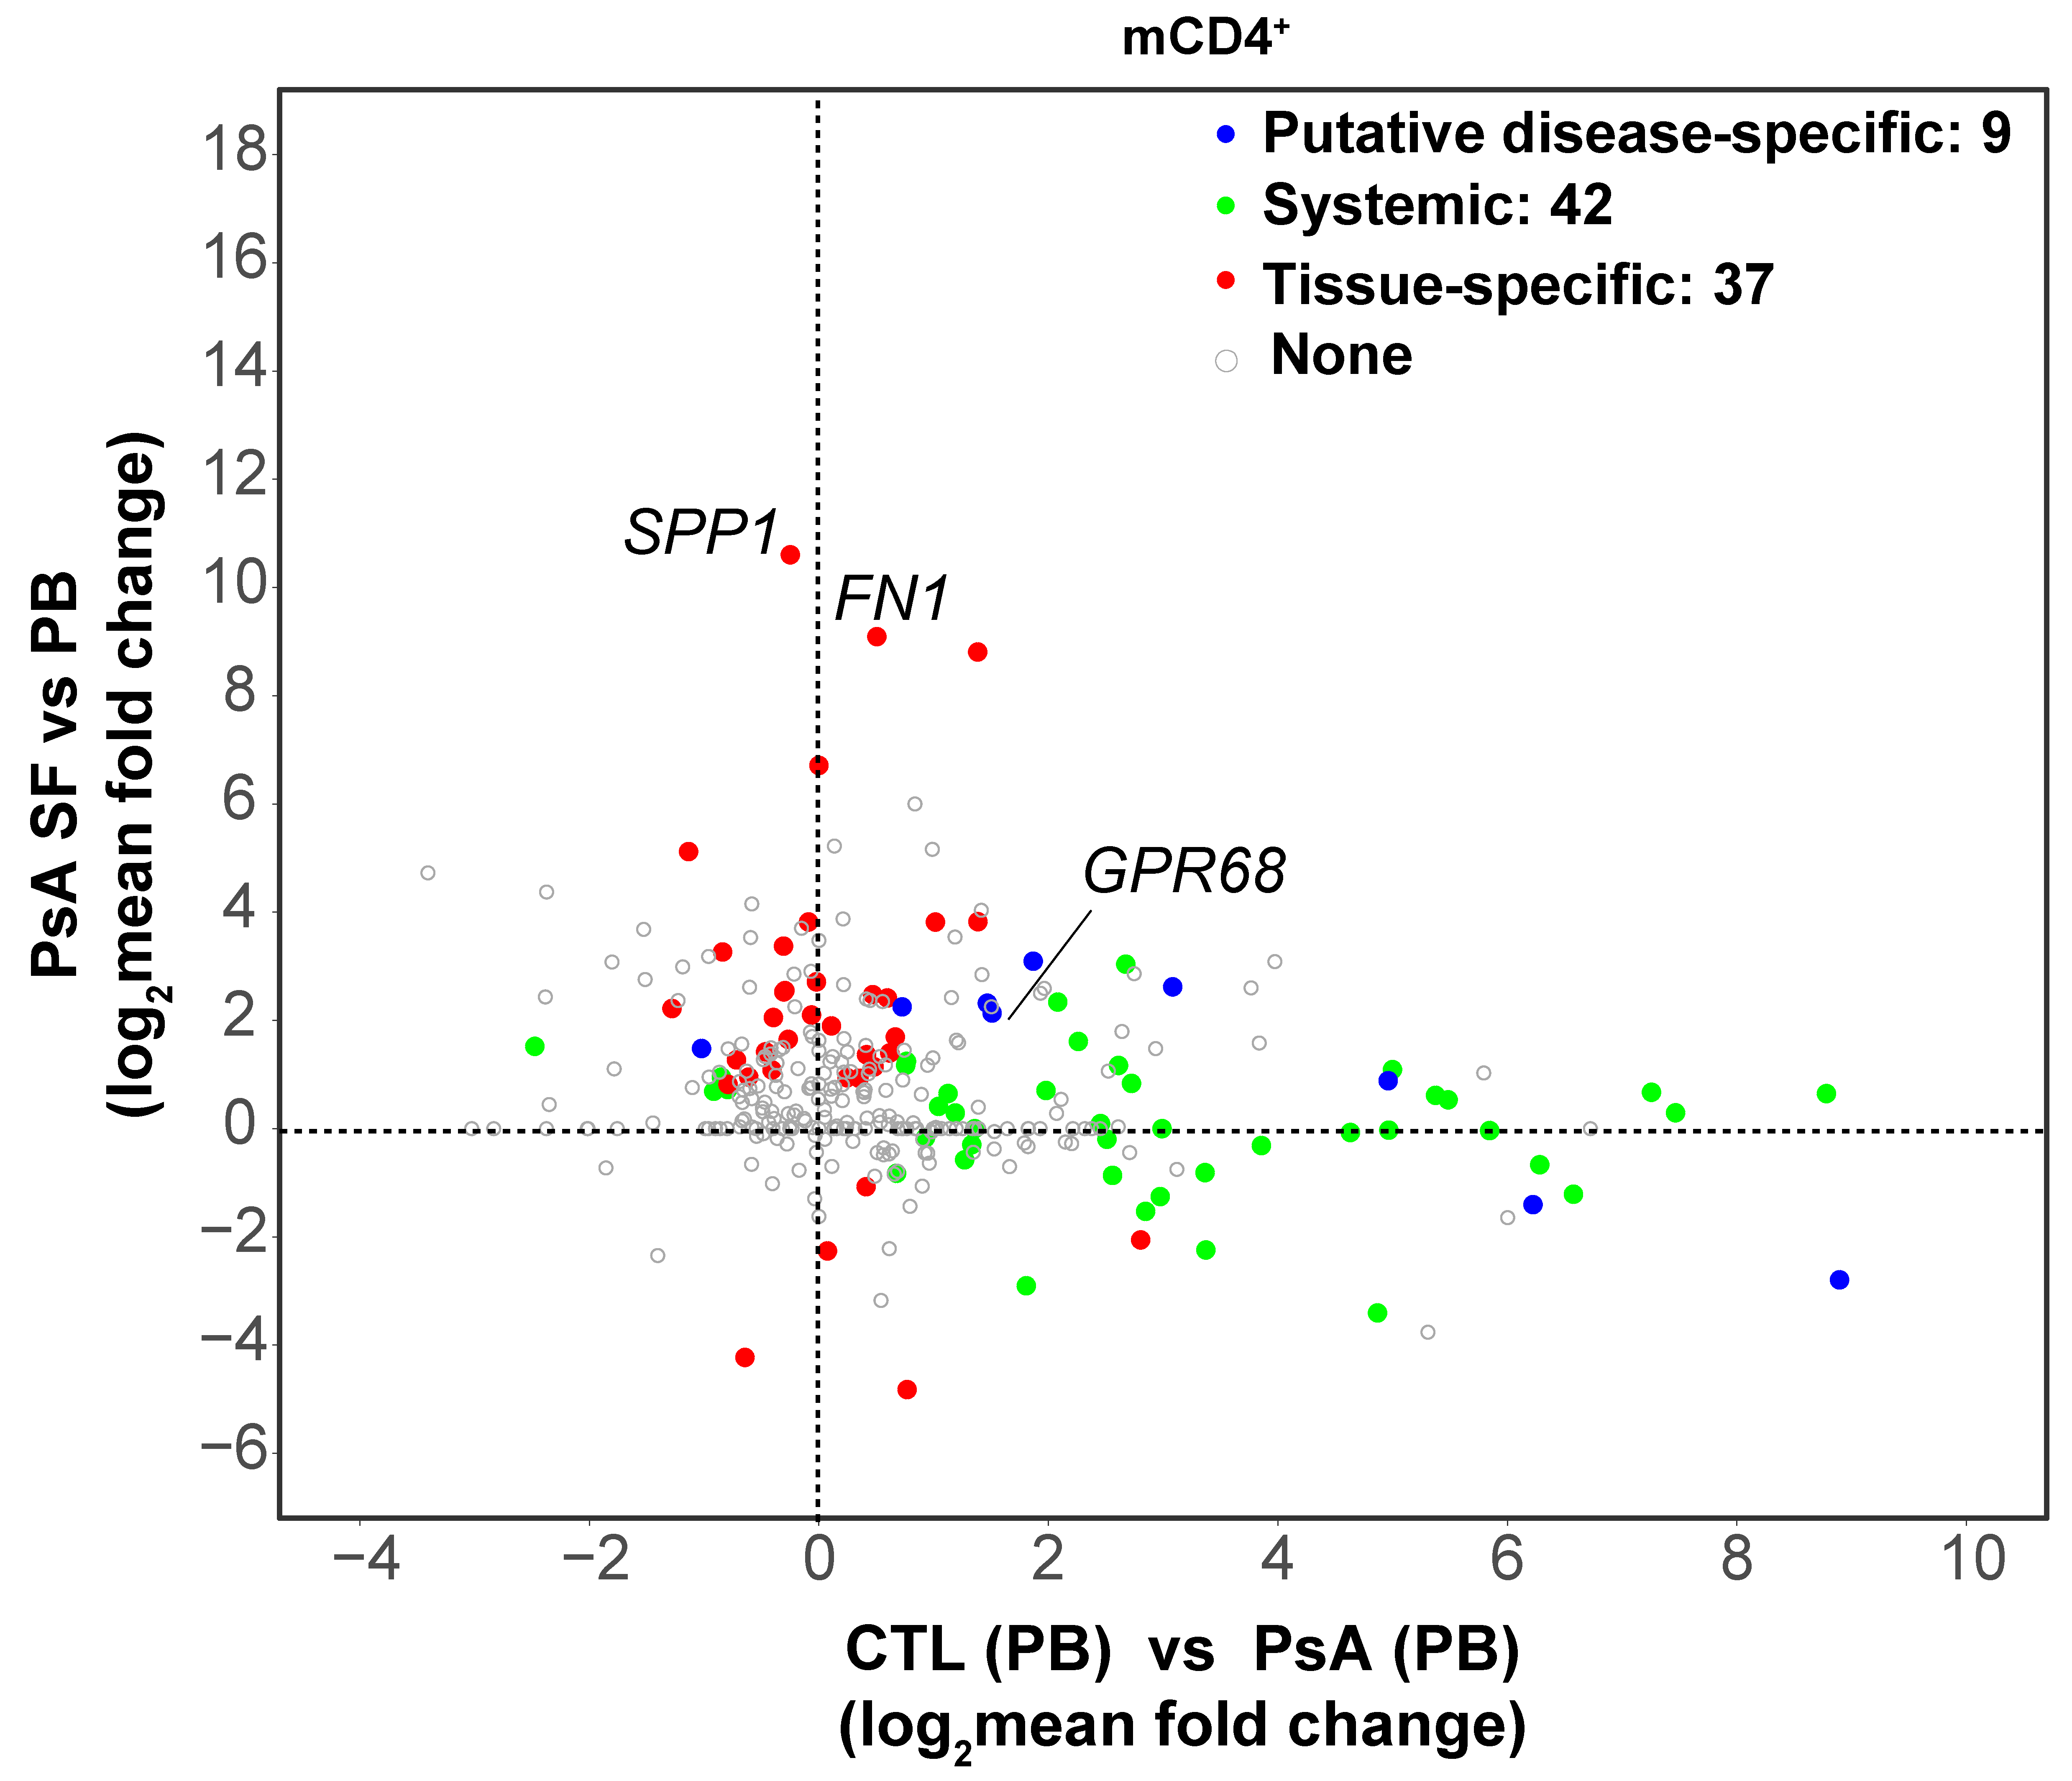
\includegraphics[width=\textwidth]{./Results3/pdfs/PSA_array_correlation_CD4_FC_HVPsA_vs_SFPBPsA}
\caption{\textbf{}}
\end{subfigure} %
\begin{subfigure}{0.45\textwidth}
\centering
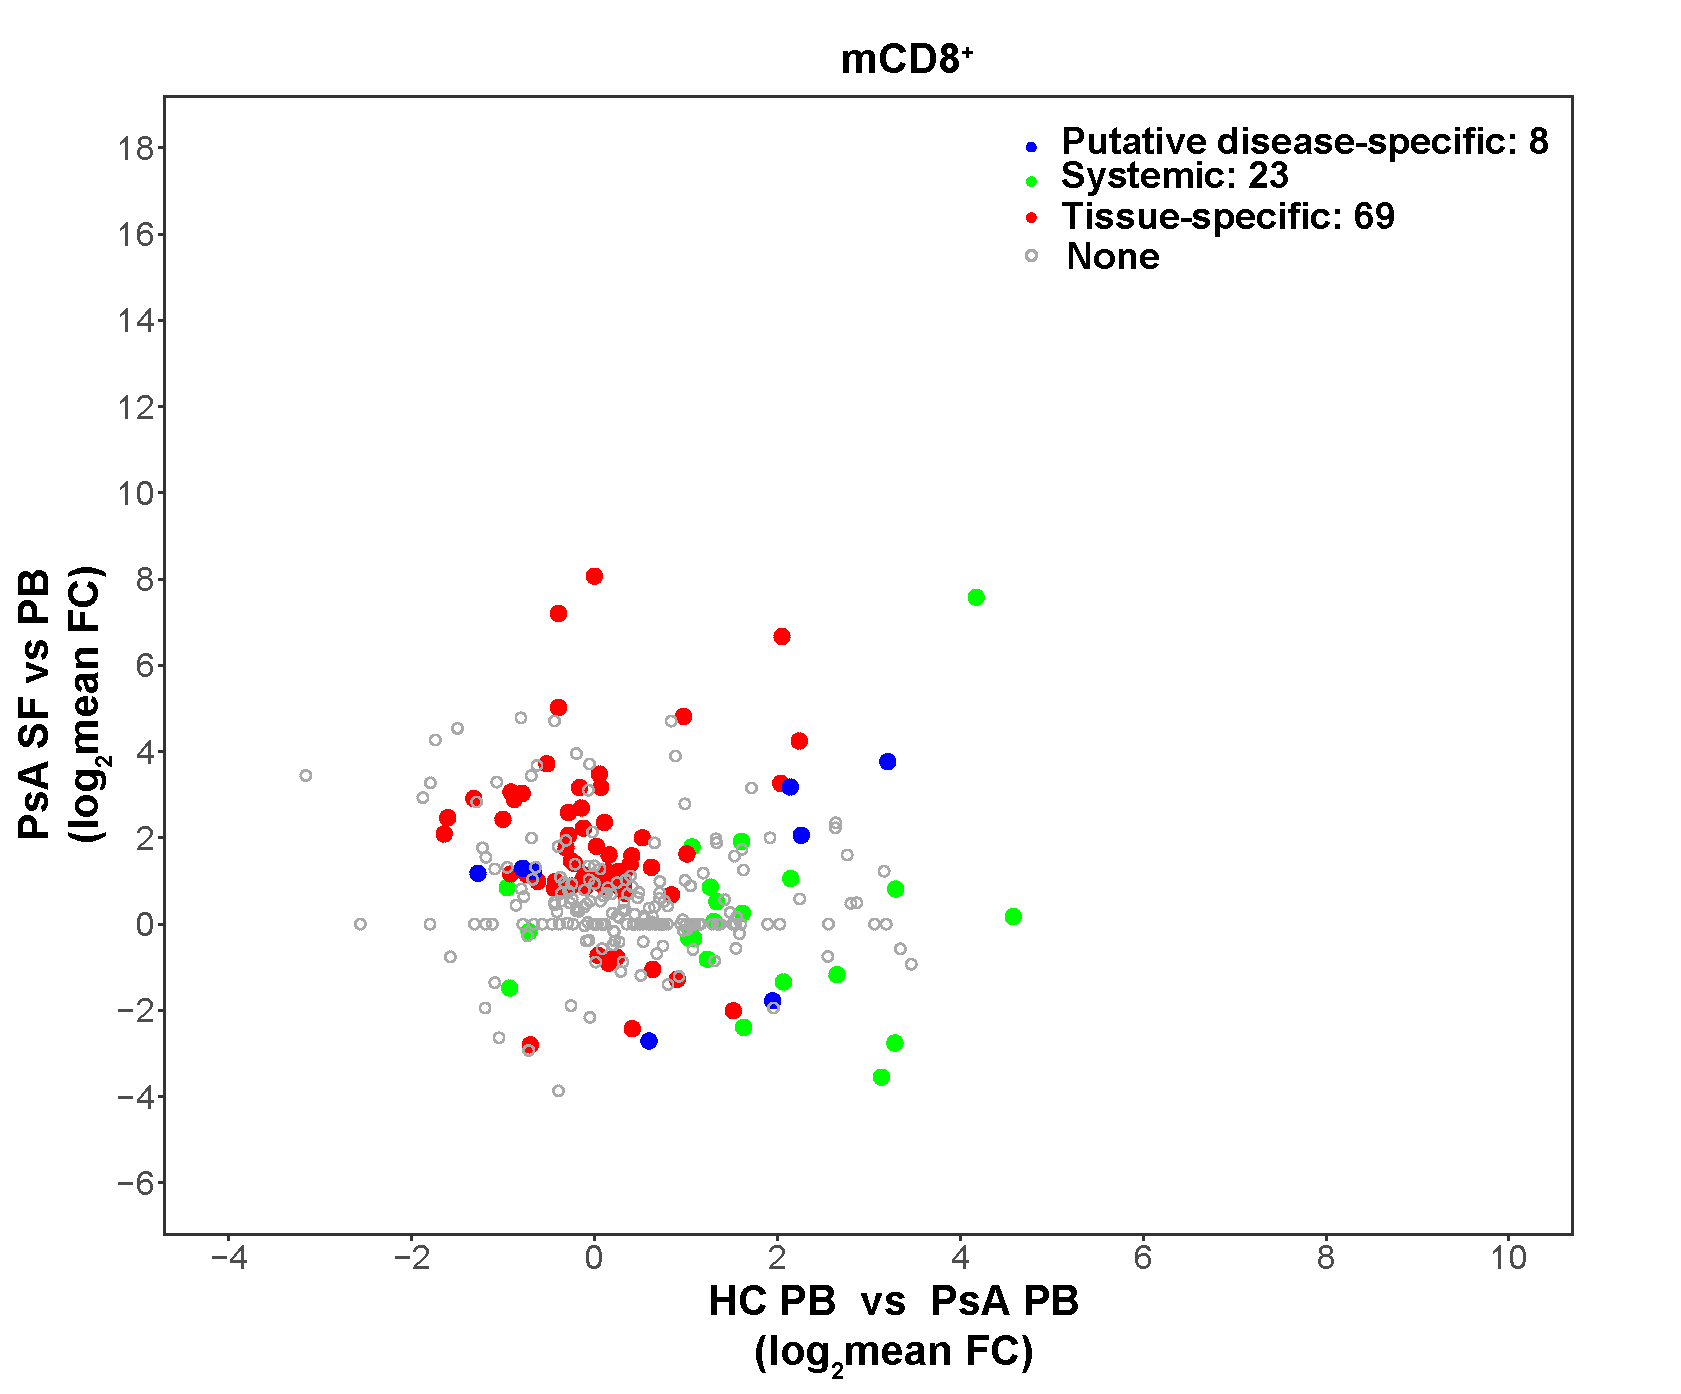
\includegraphics[width=\textwidth]{./Results3/pdfs/PSA_array_correlation_CD8_FC_HVPsA_vs_SFPBPsA}
\caption{\textbf{}}
\end{subfigure}
\caption[Comparison of immune-relevant gene expression modulation across PsA tissues (SF vs PB) and in PsA patients verus healthy controls.]{\textbf{Comparison of immune-relevant gene expression modulation across PsA tissues (SF vs PB) and in PsA patients verus healthy controls.} The qPCR log${_2}$ mean FC for each of the genes in the PsA SF vs PB contrast are plotted against the log${_2}$ mean FC for the same genes in the PsA PB vs healthy control PB contrast in a) CD14$^+$ monocytes, b) mCD4$^+$ and c) mCD8$^+$ cells. The genes are colour-coded based three categories of genes built according by comparison of changes in gene modulation between the two contrasts: only significantly modulated in PB between controls and PsA (systemic genes), only significantly modulated between SF and PB in PsA patients (tissue-specific) and significantly modulated between controls and PsA patients in PB as well as between SF and PB in PsA patients (putative disease-specific).}
\label{figure:PSA_PCR_array_HC_FC_correlation}
\end{figure} 



A second group of genes were designated as tissue-specific, since they were significantly modulated between SF and PB in PsA patients but did not show significant changes between controls and PsA at the circulating level (Figure \ref{figure:PSA_PCR_array_HC_FC_correlation} red dots). Interestingly, in CD14$^+$ monocytes the tissue specific modulated genes considerably outnumbered the systemic ones (62 versus 14), showing a more pronounced change in the expression profile of immune genes across patients' tissues than between healthy and diseased PB (Figure \ref{figure:PSA_PCR_array_HC_FC_correlation} a red dots). For example, the aforementioned \textit{NFKB} and \textit{MYD88}, \textit{TLR2} genes were only up-regulated in PsA SF CD14$^+$ monocytes and their expression was not significantly modulated between healthy controls and PsA circulating CD14$^+$ monocytes.  Similarly to CD14$^+$ monocytes, mCD8$^+$ cells also presented greater disease tissue-specific modulation than genes differentially expressed when compared to controls in PB (Figure \ref{figure:PSA_PCR_array_HC_FC_correlation} c red dots). For all three cell types, the two genes presenting the greatest FC between SF and PB \textit{SPP1} and \textit{FN1} appeared to be tissue-specific genes and no significant changes in PB between PsA and healthy controls were identified.
%Some more biology?
% talk about limitations in acknowledging these genes as dissease-tissue specific due to the fact that we don't know if they also change between PB and Sf in HV

The third category comprised genes significantly modulated for each cell type between controls and PsA patients in PB as well as between SF and PB in PsA patients. These genes defined as putative disease-specific genes presented similar numbers across CD14$^+$ monocytes, mCD4$^+$ and mCD8$^+$ (10, 9 and 8, respectively) (Figure \ref{figure:PSA_PCR_array_HC_FC_correlation} blue dots in a, b and c). In CD14$^+$ monocytes two of those genes, \textit{GPI} and \textit{PRG2}, were up-regulated in both comparisons, with further exacerbation in SF (Figure \ref{figure:PSA_PCR_array_HC_FC_correlation} a). Evidence of the glucose-6-phosphate isomerase \textit{GPI} up-regulation in disease has been found in RA synovial fibroblasts and linked to increased levels of TNF-$\alpha$ and IL-1$\beta$ in the synovium \parencite{Zhong2015}. % GPI fibroblasts https://www.ncbi.nlm.nih.gov/pmc/articles/PMC4422595/
Another example of exacerbated up-regulation in SF was the expression of \textit{GPR68} in mCD4$^+$. This gene was up-regulated in PsA PB mCD4$^+$ when compared to the control counterparts and further up-regulated in SF when compared to PB in PsA individuals (Figure \ref{figure:PSA_PCR_array_HC_FC_correlation} b). %\textit{GPR68} is a G protein-coupled receptor, expressed in T cells, amongst other cells, that undergoes activation through pH acidification, characteristic of synovial tissues under inflammation \parencite{Biniecka2016}. \textit{GPR68} activation leads to an increase of Ca$^2$$^+$ levels and subsequent activation of immune-related pathways \parencite{Saxena2011}. 
\textit{GPR68} was also up-regulated in SF compared to PB in mCD8$^+$ cells, reinforcing the relevance of this gene in the synovial pathophysiological aspect of PsA. Amongst the genes presenting an opposite behavior is the epidermal growth factor-like amphiregulin (\textit{AREG}), which in mCD8$^+$ is significantly up-regulated in PsA PB compared to the controls but is down-regulated in PsA individuals when comparing SF versus PB (Figure \ref{figure:PSA_PCR_array_HC_FC_correlation} c). %\textit{AREG} deficiency in mouse models have shown an impaired immunosupressive response by Treg cells \parencite{Zaiss2013}, which could be contributing to the exacerbated immune response in the synovium. 
% GPR68 https://ard.bmj.com/content/73/Suppl_2/511.2
%GPR68 Hypoxia Positively Regulates the Expression of pH-Sensing G-Protein–Coupled Receptor OGR1 (GPR68)
%talk about limitations of those genes to be identified as disease specific. This would need an additional comparison between HV SF and PsA SF to make sure that those genes are not modulated in SF of HV and therefore are a lanmark of disease in both tissues
Despite the interesting aforementioned findings, the identification of disease-specific and disease tissue-specific genes is clearly limited by the impossibility of obtaining healthy controls SF to include in the experimental design. 

When performing pathway enrichment analysis using the significantly modulated genes between healthy controls and PsA patients PB in the qPCR array, only the Reactome immune system pathway appeared as significant for CD14$^+$ monocytes and mCD4$^+$ cells. This result reinforced the tissue-specificity of the pathways enriched for the modulated genes between SF and PB in CD14$^+$ monocytes PsA patients and clearly suggest a more pronounced inflammatory phenotype of the pathological CD14$^+$ monocytes in SF compared to PB.



\subsection{Characterisation of the CD14$^+$ monocyte heterogeneity in PsA using scRNA-seq}
According to the analysis of chromatin accessibility and immune-related gene expression in this pilot cohort, the CD14$^+$ monocytes showed the greatest changes in chromatin accessibility and the most reliable modulation of expression for pro-inflammatory chemokines and cytokines between PB and SF. Monocytes are very plastic cells which initiate differentiation into macrophages at the site of inflammation. Therefore, exploring differences at the single-cell level may identify subpopulations with particular phenotypes of interest and may also highlight differences in the immune response driven by this cell type in circulation and at the inflamed synovium.


\subsubsection{scRNA-seq reveals two main subpopulations in SF and PB combined CD14$^+$ monocytes}
%Explain how I did the analysis
ScRNA-seq was performed in paired PBMCs and SFMCs isolated from three PsA patients (Table \ref{tab:PSA_datasets_per_sample}). scRNA-seq data from each of the PBMCs and SFMCs samples, were filtered as explained in \ref{ch:Mat} and CD14$^+$ monocytes were subset from the rest of cell populations by expression of \textit{CD14} and \textit{LYZ}, two of the most accurate expression markers defining this cell population (Figure \ref{figure:PsA_scRNAseq_SF_an_PB_monocytes_identification_from_bulk} a and b). Across all six samples (three SFMCs and three PBMCs), 2,459 cells were CD14$^+$ monocytes cells, representing approximately 17\% of the bulk SFMCs and PBMCs cells included in the analysis and in line with the proportion of CD14$^+$ monocytes previously reported using cell surface markers by mass cytometry  (Figure \ref{figure:PsA_cell_composition}). The CD14$^+$ monocytes identified in each of the three  paired PBMCs-SFMCs PsA samples were combined using CCA to correct for intrinsic batch effect, unavoidable due to patient samples recruitment in different days and generation of SFMCs and PBMCs 10X libraries separately. CCA alignment of the six CD14$^+$ monocytes populations was followed by conservative unpervised clustering (using resolution 0.1) and t-SNE visualisation. 

\bigskip
\begin{figure}[H]
\centering
\begin{subfigure}[b]{0.60\textwidth}
\centering 
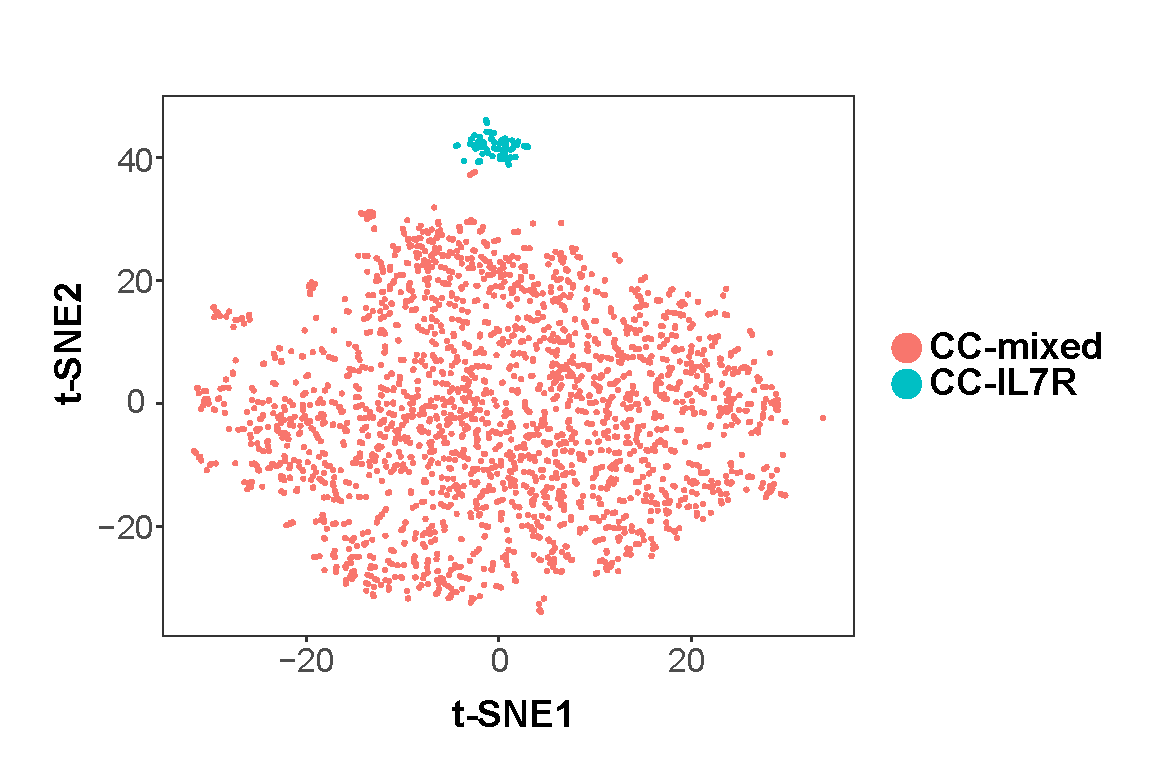
\includegraphics[width=\textwidth]{./Results3/pdfs/PSA_scRNAseq_tSNE_CC_mixed_and_IL7R}
\caption{}
\end{subfigure}
~
\begin{subfigure}[b]{0.75\textwidth} 
%the [b] prevents offset in subcaptions
\centering
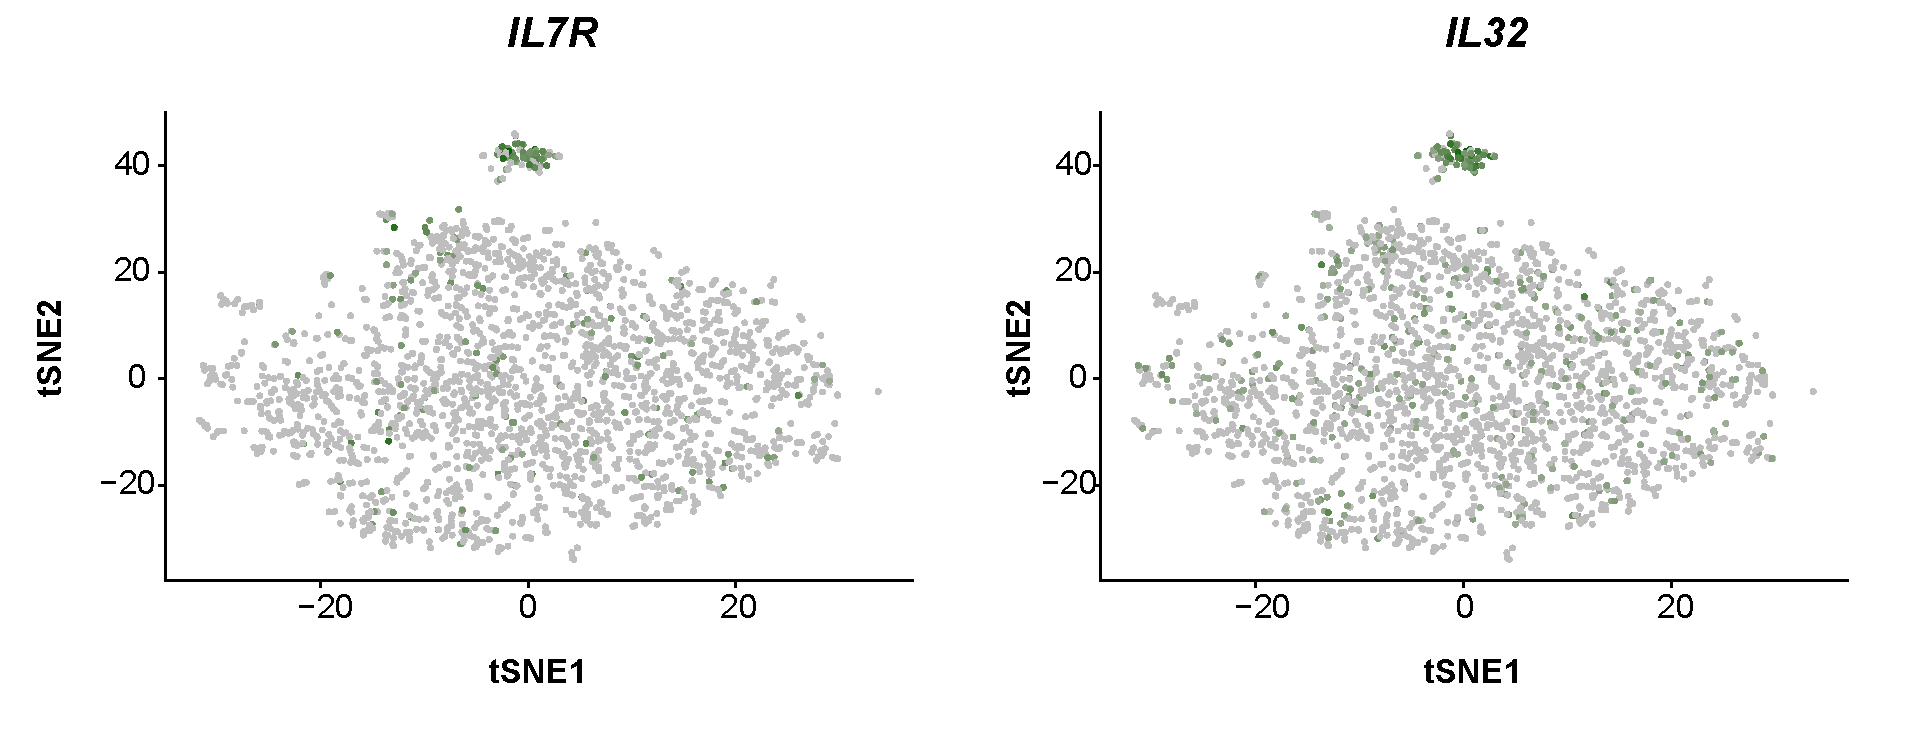
\includegraphics[width=\textwidth]{./Results3/pdfs/PSA_scRNAseq_CC_mixed_and_IL7R_overlay_markers}
\caption{}
\end{subfigure}
\caption[Identification of two main CD14$^+$ monocytes subpopulations in the SF and PB combined analysis]{\textbf{Identification of two main CD14$^+$ monocytes subpopulations in the SF and PB combined analysis.} a) Visualisation using t-SNE dimensional reduction of the two cluster (CC-mixed and CC-IL7R) identified in the combined SF and PB CD14$^+$ monocyte cells using a very conservative resolution (res=0.1) for the unsupervised clustering analysis. Ech of the dots represents a cell, colour-coded by the cluster membership (pink=CC-mixed and turquoise=CC-IL7R). b) Overlap of \textit{IL7R} and \textit{IL32} expression intensities (green) on the t-SNE representation of the SF and PB CD14$^+$ monocytes.\textit{IL32} and \textit{IL7R} gene expression appeared as markers for the CD14$^+$ monocytes from the CC-IL7R cluster.}
\label{figure:PsA_scRNAseq_SF_an_PB_monocytes_identification_from_bulk}
\end{figure}

%Say that using a conservative approach to find cluster two main groups were identified: No IL7R vs IL7R
%Probably more heterogeneity could be found within the big cluster but given number of replicates and intensive analysis required to make sure clusters are estable we decided to only trust these two main groups
Using this conservative approach for cluster definition, two robust clusters were identified (Figure \ref{figure:PsA_scRNAseq_SF_an_PB_monocytes_identification_from_bulk} a). The smallest cluster, named a CC-IL7R, was characterised by the expression of \textit{IL7R}, \textit{IL32} and \textit{CCL5}, amongst others, and was formed by a total of 72 cells (43 from SF versus 29 from PB) (Figure \ref{figure:PSA_scRNAseq_CC_mixed_and_IL7R_overlay_markers} b and \ref{figure:PSA_scRNAseq_CC_mixed_and_IL7R_markers_heatmap}) (\parencite{Al-Mossawi2018}, in revision). The proportion of IL7R$^+$CD14$^+$ monocytes when compared to the totalCD14$^+$ monocyte population was very similar in SF and PB (3 and 2.7\%, respectively) in this data. The largest cluster, named as CC-mixed, consisted of 2,387 (1,356 SF and 1,031 PB). CC-mixed was an heterogeneous cluster, without consistent expression pattern for those genes identified as cluster markers (Figure \ref{figure:PSA_scRNAseq_CC_mixed_and_IL7R_markers_heatmap}). When using a less conservative approach for cluster definition by increasing the resolution (resolution 0.4, 0.6 and 0.8), additional clusters were identified. Similarly to the observation in the most conservative approach, no consistency was found in the expression of the top genes defined as markers by cells of the same cluster (data not shown). Due to the moderate cohort size, limitation in accounting for batch effect for cluster identification and the complexity in the definition and identification of stable clusters this analysis could only yield limited information about monocytes subpopulations.  Increasing cohort size and a implementation of more exhaustive analysis and alternative methods could lead to identification of additional subpopulations within the combined SF and PB CD14$^+$ monocytes in the CC-mixed cluster (see \ref{Discussion_scRNAseq}). For the scope of this project, downstream analysis, including DGE between the two tissues, was performed in the CC-mixed and CC-IL7R clusters identified by the most conservative approach (resolution 0.1).




\subsubsection{Differential gene expression between SF and PB CD14$^+$ monocytes in CC-mixed and CC-IL7R}
%DGE was performed between tissues within each cluster
DGE analysis was performed in order to explore differences between SF and PB within each of these two main CD14$^+$ monocyte subpopulations. For the CC-mixed cluster, a total of 251 genes were differentially expressed at an FDR$<$0.01 and FC$>$1.5 between SF and PB, of which 149 and 102 presented up- and down-regulation, respectively (Figure \ref{figure:PsA_scRNAseq_vulcano_plots_mixed_and_IL7R_clusters} a). Differential analysis within the CC-IL7R cluster revealed a total of 37 modulated genes, with the majority (35 out of 37) up-regulated in SF compared to PB (Figure \ref{figure:PsA_scRNAseq_vulcano_plots_mixed_and_IL7R_clusters} a). Due to the low number of cells in the CC-IL7R cluster and the limited sample size (n=3), the analysis only identified as significantly differentially expressed (FDR$<$0.01) genes presenting FC$>$1.5. Out of the 37 DEGs in the CC-IL7R cluster between the two tissues, 30 were also shared by the CC-mixed cluster. The seven distinctly modulated genes in the CC-IL7R cluster included \textit{CD44} (receptor of the protein product of \textit{SPP1}), \textit{MT-CO2} or S-ribosomal protein (RPS) genes (\textit{RPS29} and \textit{RPS27}). 


\bigskip
\begin{figure}[H]
\centering
\begin{subfigure}[b]{0.55\textwidth}
\centering 
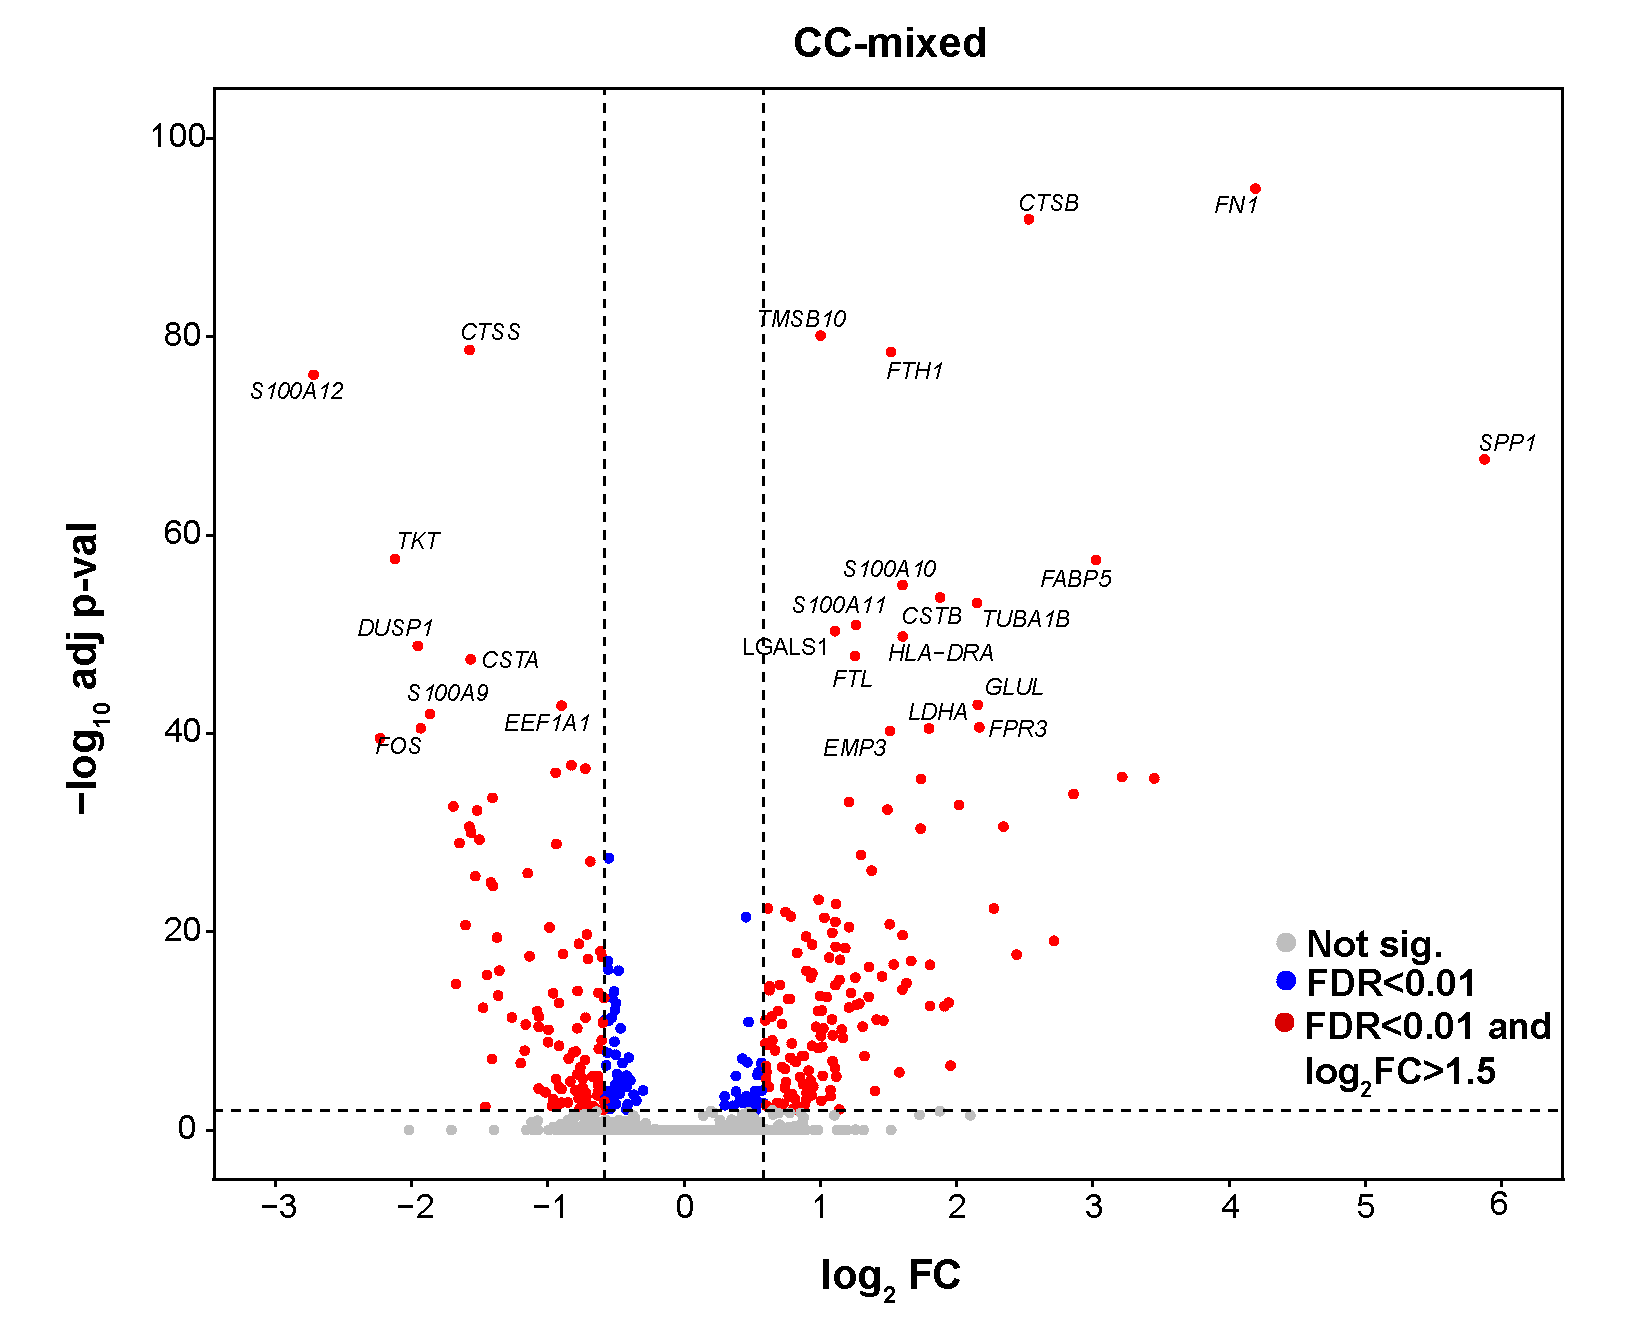
\includegraphics[width=\textwidth]{./Results3/pdfs/PSA_10X_all_combined_aligned_monocytes_DGE_SF_vs_PB_cluster_0_vulcano_plot}
\caption{}
\end{subfigure}
~
\begin{subfigure}[b]{0.55\textwidth} 
%the [b] prevents offset in subcaptions
\centering
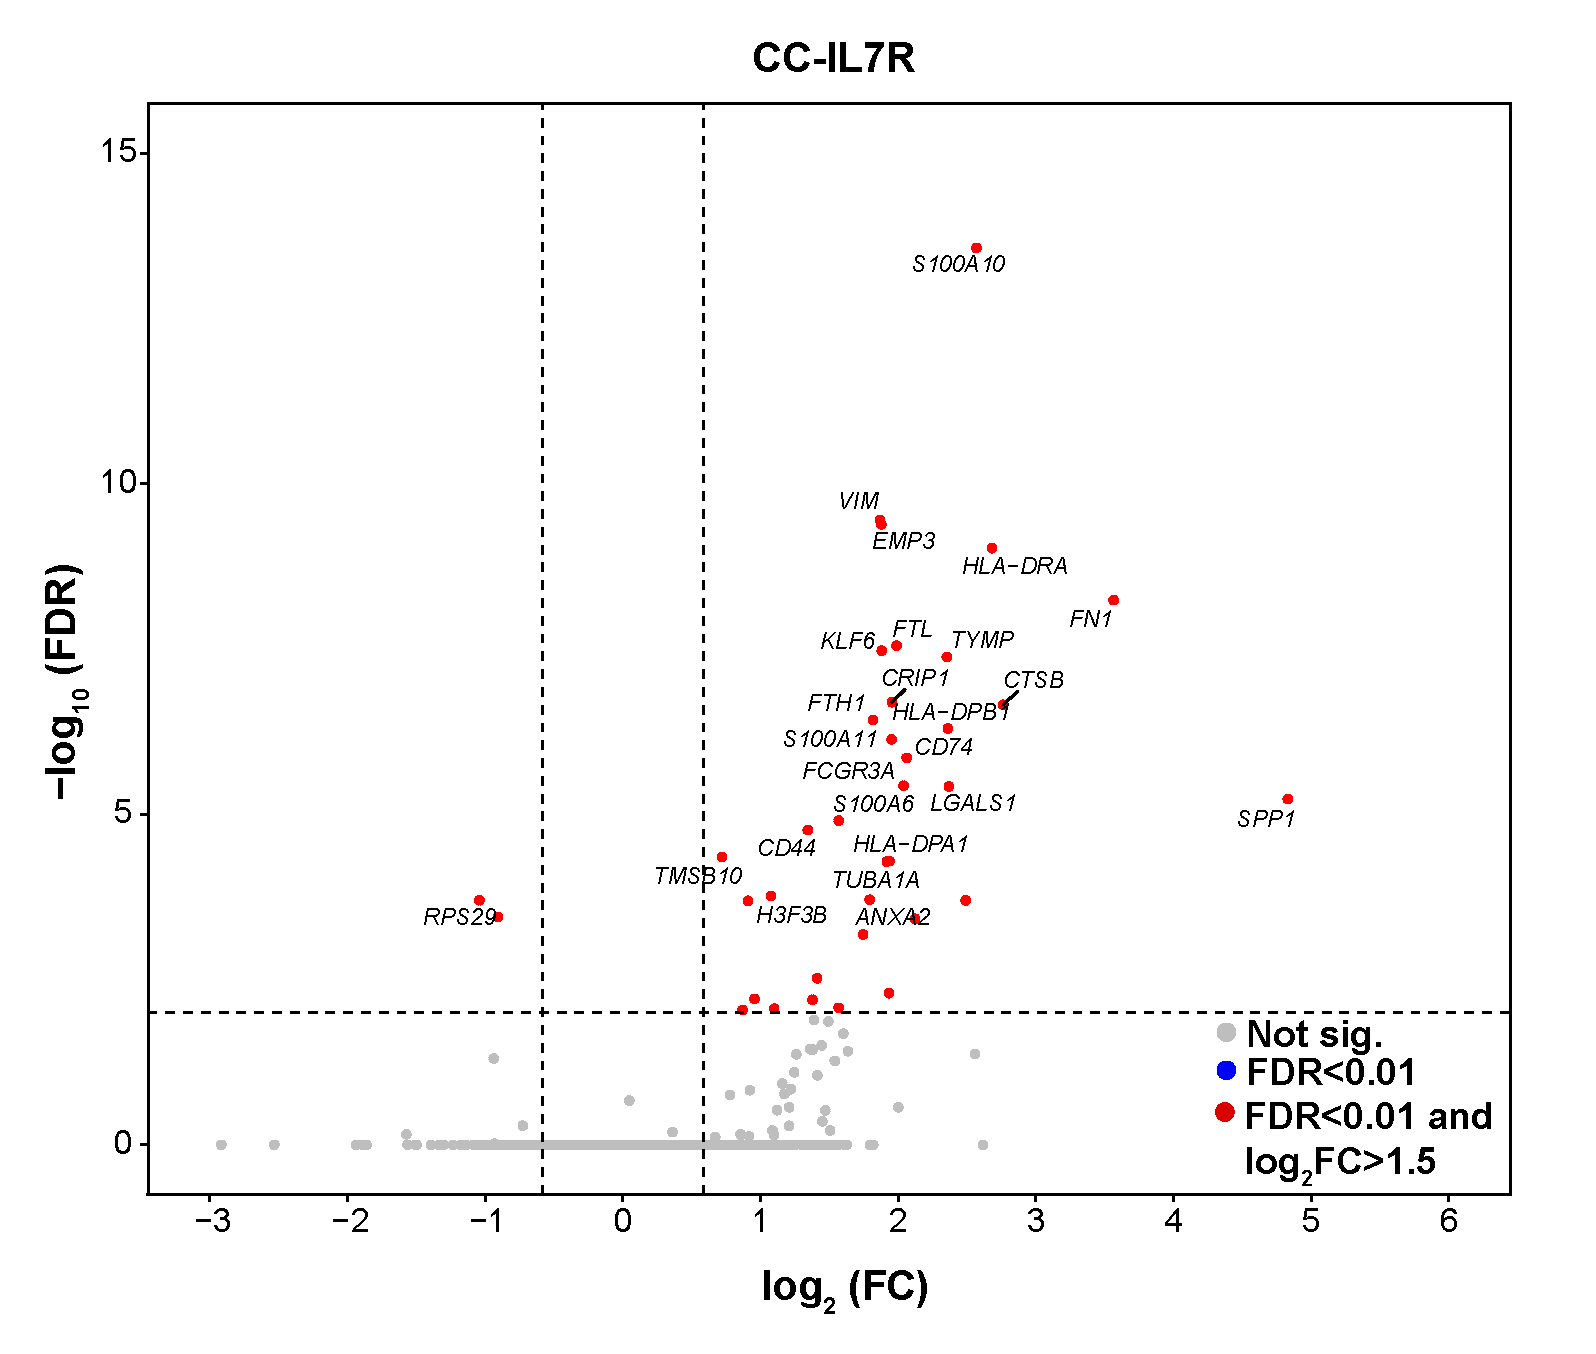
\includegraphics[width=\textwidth]{./Results3/pdfs/PSA_10X_all_combined_aligned_monocytes_DGE_SF_vs_PB_IL7R_vulcano_plot}
\caption{}
\end{subfigure}
\caption[Sc-RNA-seq differential gene expression results between SF and PB in the CC-mixed and CC-IL7R CD14$^+$ monocytes subpopulations.]{\textbf{Sc-RNA-seq differential gene expression results between SF and PB in the CC-mixed and CC-IL7R CD14$^+$ monocytes subpopulations.} Vulcano plots showing differences in gene expression between SF and PB a) CC-mixed and b) CC-IL7R CD14$^+$ monocyte cluster. In a and b, the significance (log${_10}$FDR) of the differential expression (y-axis) is plotted against the log${_2}$FC. A positive FC indicates higher expression in CD14$^+$ monocytes from SF compared to PB. Genes showing FDR$<$0.01 are coloured in blue and genes presenting and FDR$<$0.01 and FC$>$1.5 are coloured in red. The most significant genes are labelled.}
\label{figure:PsA_scRNAseq_vulcano_plots_mixed_and_IL7R_clusters}
\end{figure}



Comparison with the qPCR expression analysis revealed a modest overlap between the two assays, particularly for the DEGs in the CC-IL7R. Amongst the 72 DEGs (pval$<$0.05) detected by qPCR between SF and PB in CD14$^+$ monocytes, only 12 and 4 genes were also differentially expressed (FDR$<$0.01 and no FC threshold) in the CC-mixed and CC-IL7R clusters, respectively (Figure \ref{:figure:PsA_scRNAseq_qPCR_ATAC_correlation} a). Genes with reproducible differential expression between SF and PB by the two approaches included genes with the largest FCs in both assays, such as \textit{SSP1}, \textit{FN1}, \textit{OLR1} and \textit{S100A12}, being the direction of change also consistent for all of them. %add something about cell type specificity
%Regarding the low number of qPCR DEGs between SF and PB in total CD14$^+$ monocytes reproduced by the scRNA-seq in any of the two main clusters identified could be explained by the differences in the cell sorting (FACS versus \textit{in silico} expression markers), the low number of replicates for each assay as well as different sensitivity of the two technologies. 
%The limited overlap between qPCR and scRNA-seq DEGs could also partly explain the absence of overlap between enriched pathways across the two gene expression analysis. 
   
\bigskip
\begin{figure}[H]
\centering
\begin{subfigure}[b]{0.50\textwidth}
\centering 
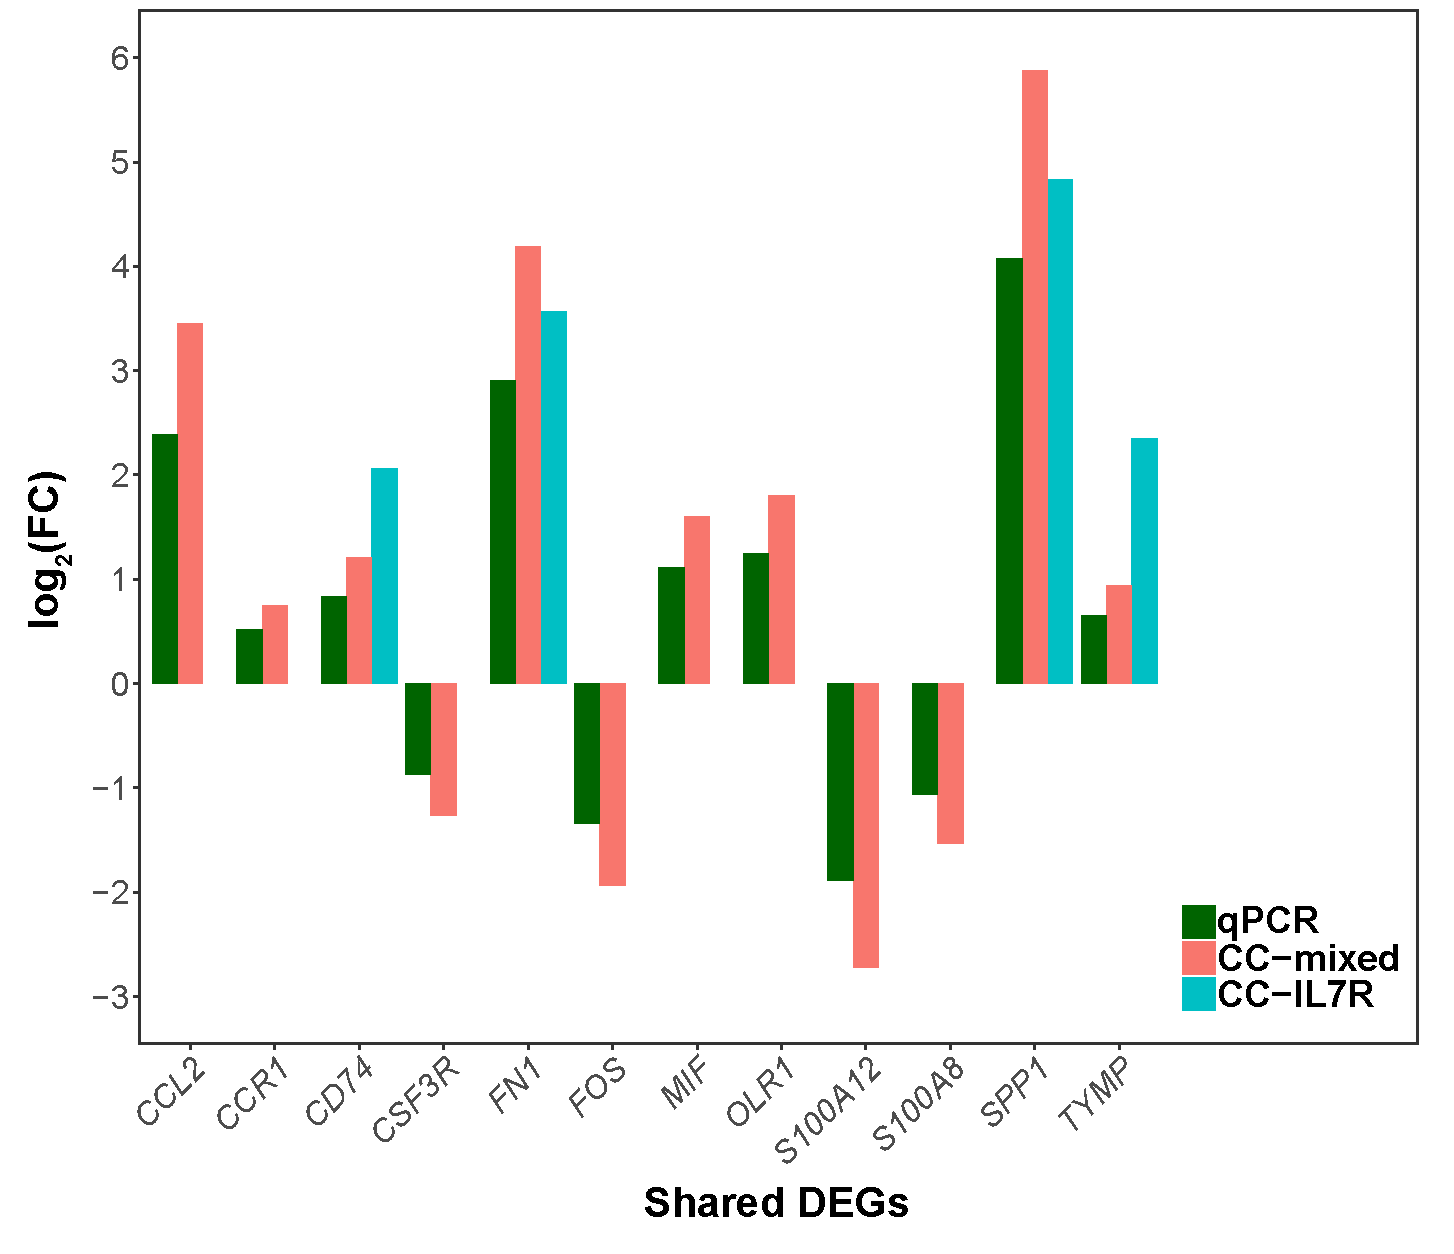
\includegraphics[width=\textwidth]{./Results3/pdfs/PSA_scRNAseq_PCR_array_overlapping_genes_log2FC}
\caption{}
\end{subfigure}
~
\begin{subfigure}[b]{0.70\textwidth} 
%the [b] prevents offset in subcaptions
\centering
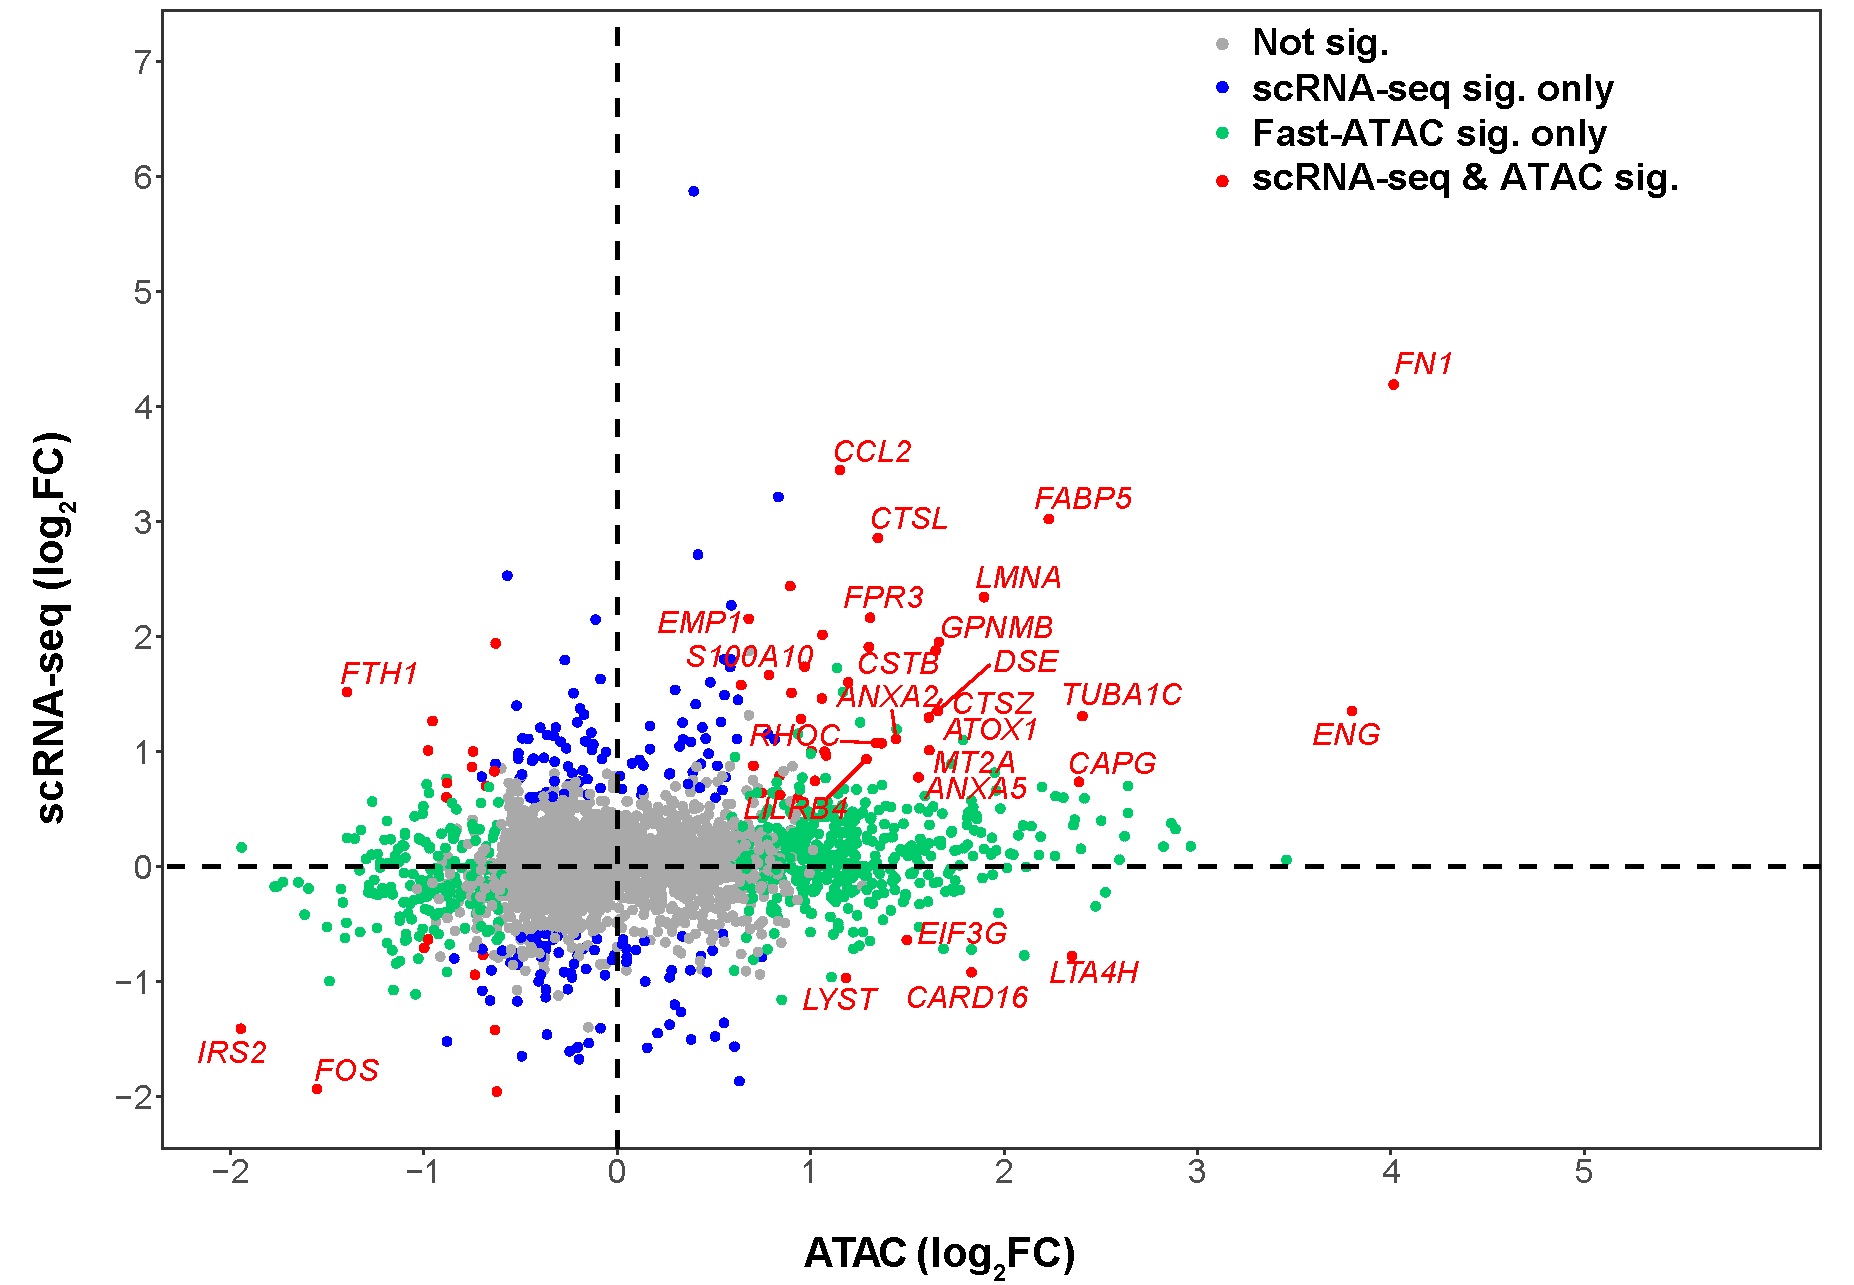
\includegraphics[width=\textwidth]{./Results3/pdfs/PSA_ATAC_scRNA_CD14_correlation_plot}
\caption{}
\end{subfigure}
\caption[Correlation between scRNA-seq, qPCR and chromatin accessibility in PsA CD14$^+$ monocytes.]{\textbf{Correlation between scRNA-seq, qPCR and chromatin accessibility in PsA CD14$^+$ monocytes.} a) Overlap between the scRNA-seq DEGs (significant based only on FDR$<$0.01) from the CC-mixed and CC-IL7R CD14$^+$ monocyte cluster in SF versus PB and the corresponding DEGs (pval<0.05) detected by qPCR in the bulk CD14$^+$ monocytes population. For each of the shared DEGs, the log$_2$FCs from the qPCR and the 10X scRNA-seq analysis are represented. b) Correlation plot comparing SF and PB differences in scRNA-seq expression of the CC-mixed CD14$^+$ monocytes and ATAC chromatin accessibility in total CD14$^+$ monocytes. The log$_2$FCs for scRNA-seq differential expression of all transcripts in the CC-mixed CD14$^+$ monocytes are plotted against the log$_2$FC for total CD14$^+$ monocytes ATAC differential chromatin accessibility analysis in regions proximal ($\leq$5Kb) to the same genes. Blue colouring indicates significant differential expression in scRNA-seq only; green represents ATAC significant DAR only; red indicates significant differential expression and chromatin accessibility; grey indicates no significant differential expression or chromatin accessibility in CD14$^+$ monocytes. Significance is based on FDR and FC thresholds (FDR$<$0.01 and FC$>$1.5) in both assays.}
\label{figure:PsA_scRNAseq_qPCR_ATAC_correlation}
\end{figure}


%Interestingly, latest studies have involved RPS proteins in immune signalling and modulation of the NF-$\kapa$B response \parencite{Zhou2015}


% Pathway analysis
Pathway enrichment analysis was performed for the significantly DEGs between SF and PB in the CC-mixed and CC-IL7R subpopulations. The DEGs in the CC-mixed cluster were significantly enriched (FDR$<$0.01) a number of pathways (Table \ref{tab:PSA_scRNAseq_CD14_DEGs_pathway_analysis} and \ref{tab:PSA_scRNAseq_CC_mixed_and_IL7R_additional_pathways}), some of them of particular pathological relevance (Table \ref{tab:PSA_scRNAseq_CD14_DEGs_pathway_analysis}). 

\begin{table}[htbp]
%\setlength{\tabcolsep}{20pt} only to stretch the columns if you want
%\renewcommand{\arraystretch}{1.5}
\centering
\begin{tabular}{@{} c c c}
\toprule
\textbf{Cluster} & \textbf{Pathways} \\
\midrule
\midrule
         & Ag processing and presentation via MHC-II \\
				 & Extracellular matrix and extracellular \\
				 & matrix-associated proteins \\
CC-mixed & Phagosome and lysosome formation \\
				 & IFN signalling \\
				 & Cytokine signalling $^\ast$ \\
				 & Apoptosis \\
				 & Innate immunity \\
\midrule				
         & Adaptive immunity \\
         & Ag processing and presentation \\
CC-IL7R	 & Phagosome \\
         & Extracellular matrix and extracellular \\
				 & matrix-associated proteins \\
\bottomrule
\end{tabular}
\medskip %gap
\caption[Most relevant enriched pathways for the DEGs between SF and PBCD14$^+$ monocytes in CC-mixed and CC-IL7R.]{\textbf{Most relevant enriched pathways for the DEGs between SF and PBCD14$^+$ monocytes in CC-mixed and CC-IL7R.} Significantly DEGs based on the FDR and FC threhold were used for the analysis. Most relevant enriched pathways based on FDR$<$0.01. ($^\ast$) Enrichment for FDR$<$0.05. Additional pathways included in Table \ref{tab:PSA_scRNAseq_CC_mixed_and_IL7R_additional_pathways}.}
\label{tab:PSA_scRNAseq_CD14_DEGs_pathway_analysis}
\end{table}


One of those pathways was for the Ag processing and presentation pathway, contributed by up-regulated expression in SF CD14$^+$ monocytes of \textit{CD74} and genes from the \textit{HLA-D} family such as \textit{HLA-DQA1} and \textit{HLA-DRB1} (Table \ref{tab:PSA_scRNAseq_CD14_DEGs_pathway_analysis}). Enrichment for IFN signalling was driven differential expression of genes such as \textit{IFI6}, \textit{IFITM3}, \textit{ISG15} and the TF \textit{STAT1}, all of them up-regulated in SF when compared to PB CD14$^+$ monocytes. Another relevant enriched pathway was the extracellular matrix and extracellular matrix-associated proteins, which involve genes of the S100 family (including \textit{S100A8}, \textit{S100A9}, \textit{S100A10}, \textit{S100A11} and S100A12, that interact with the receptor for advance glycosylation end products (RAGE) and induce production of matrix-degrading enzymes. The phagosome and lysosome formation pathway also appeared to be more active in SF CD14$^+$ monocytes, with up-regulation of genes such as \textit{CTSL}, which is involved in protein degradation in lisosomes and phagocytosis of apoptotic cells. Lastly, enrichment for cytokine signalling was not driven by differential expression of cytokines but was contributed by up-regulation of pro-inflammatory TFs such as \textit{STAT1}, amongst other genes. The most functionally relevant significantly enriched pathways identified for DEGs in the CC-IL7R subpopulation were common to the ones found in the CC-mixed cluster (Table \ref{tab:PSA_scRNAseq_CD14_DEGs_pathway_analysis}).



\subsubsection{Moderate genome-wide correlation correlation between chromatin accessibility and scRNA-seq expression in the CC-mixed cluster}
In order to determine the overall correlation between scRNA-seq expression and chromatin accessibility, comparison between the log$_2$FCs for all the expressed genes in the CC-mixed CD14$^+$ monocytes cluster and all the accessible chromatin regions in bulk CD14$^+$ monocytes between SF and PB was conducted . Changes in expression and chromatin accessibility only presented a moderate correlation in this data (R=0.214, pval=2x10$^{-16}$)(Figure \ref{figure:PsA_scRNAseq_qPCR_ATAC_correlation} b). In the CC-mixed cluster, 64 genes out of the 251 DEGs (FDR$<$0.01 and FC$>$1.5) were proximal ($\leq5$Kb) to one or more ATAC DARs (Table \ref{tab:PSA_10X_CD14_clusters_and_ATAC_overlap}). This overlap was significant and highlighted the enrichment (Fisher exact test pval=1.5x10$^-3$) of DEGs in the CC-mixed cluster for proximal DARs identified by ATAC in bulk CD14$^+$ monocytes. The majority of the overlaps corresponded to matched increase or decrease (40 and 12 genes, respectively) of gene expression and chromatin accessibility in SF vs PB. However, 14 DEGs in the CC-mixed cluster showed opposite direction of change between expression and chromatin accessibility (Table \ref{tab:PSA_10X_CD14_clusters_and_ATAC_overlap}). 


  
\begin{table}[htbp]
%\setlength{\tabcolsep}{20pt} only to stretch the columns if you want
%\renewcommand{\arraystretch}{1.5}
\centering
\begin{tabular}{@{} c c c c}
\toprule
\textbf{Cluster} & \textbf{Up-regulated genes}        &  \textbf{Up-regulated genes }  & \textbf{Opposite direction} \\
                   & \textbf{with proximal}           &  \textbf{with proximal}      & \textbf{in expression } \\
									 &	\textbf{SF open DAR}				    &  \textbf{PB open DAR}        & \textbf{and DAR}\\
\midrule
\midrule
 CC-mixed         & 40                                       &  10                                & 14 \\
 CC-IL7R          & 9                                        &  0                                 & 4 \\
\bottomrule
\end{tabular}
\medskip %gap
\caption[scRNA-seq DEGs in SF versus PB CD14$^+$ monocytes proximal to a DAR in Fast-ATAC.]{\textbf{scRNA-seq DEGs in SF versus PB CD14$^+$ monocytes proximal to an ATAC DAR.}. For each of the two CD14$^+$ monocytes cluster identified by scRNA-seq analysis, an overlap is defined when a gene is differentially expressed (FDR$<$0.01 and FC$>$1.5) between SF and PB and a proximal significant DAR ($\leq$5Kb) showing same or opposite direction of change is also found.}
\label{tab:PSA_10X_CD14_clusters_and_ATAC_overlap}
\end{table}

Amongst the DEGs in the CC-mixed cluster overlapping a proximal DAR were \textit{CCL2} and \textit{FN1} (Figure \ref{figure:PsA_scRNAseq_qPCR_ATAC_correlation} b). Both genes were up-regulated in SF compared to PB in the CC-mixed cluster, proximal to a SF open DAR, and found up-regulated in the same direction by the qPCR expression analysis in SF bulk CD14$^+$ monocytes compared to PB (Figure \ref{figure:PsA_scRNAseq_qPCR_ATAC_correlation} a). 

Similarly to the CC-mixed results, the DEGs in the CC-IL7R cluster between SF and PB were also enriched for those genes with at least one DARs nearby (Fisher exact test pval=1.85x10$^-9$). Amongst the 22 DEGs overlapping a proximal DAR, 13 of them had correlated dysregulation of expression and chromatin accessibility only 4 presented opposite directionality in the variation of the two features (Table \ref{tab:PSA_10X_CD14_clusters_and_ATAC_overlap}). The CC-IL7R cluster and CD44 data not shown.


Overall, this results have shown only moderate correlation between gene expression and proximal chromatin accessibility, which may highlight causality to some extent for the dysregulation of the chromatin landscape in the alteration of gene expression between CD14$^+$ monocytes in the two tissues.





%The biological relevance of the IL7R does not show distinct differences in gene expression between tissues and its relevance may be related to the distinctive biological function of this subset in both tissues. Seems more abundant in SF and that would make sense with the differences in the PCR array in bulk expression.



\subsection{Mass cytometry reveals differences in protein expression consistent with the chromatin accessibility and transcriptomic profile in PsA CD14$^+$ monocytes.}

To determine the effect of chromatin accessibility and genes expression differences in CD14$^+$ monocytes between SF and PB at the protein level mass cytometry was conducted in collaboration with Dr Hussein Al-Mossawi and Dr Nicole Yager. For those samples with paired ATAC and/or qPCR expression data, intra-cellular staining for relevant cytokines was performed before and after treatment with BFA, which blocks cytokine release and enables identification of cells actively producing cytokines in absence of additional inflammatory stimuli (see Chapter \ref{ch:Mat}). Due to technical problems, only a limited number of intra-cellular cytokine staining passed QC, being TNF-$\alpha$ amongst the more relevant ones. 

Mass cytometry expression of CD14$^+$ versus TNF-$\alpha$ demonstrated greater intensity of TNF$\alpha$ staining after 6h of BFA treatment in SF (Figure \ref{figure:PsA_monocytes_percentage_TNFa} a blue dots bottom panel) when compared to PB CD14$^+$ monocytes in all three PsA patients (Figure \ref{figure:PsA_monocytes_percentage_TNFa} a blue dots top panel). Furthermore, the percentage of TNF-$\alpha$ producing cells in each tissue was quantified as the difference of TNF-$\alpha^+$ cells before and after BFA treatment for 6h (6h minus 0h). In PB, the resulting percentage of CD14$^+$ monocytes TNF-$\alpha^+$ did not surpass the 1\%, indicating a very low increment of TNF$\alpha$ producing cells after BFA treatment. Conversely, SF CD14$^+$ cells showed a larger percentage of cells actively producing TNF-$\alpha$, ranging between 1.5 and 11.8\% (Figure \ref{figure:PsA_monocytes_percentage_TNFa} b). This observation was consistent with increased chromatin accessibility nearby genes of the NF-$\kappa$B signalling pathway as well as with increased expression of a number of genes in the TLR and NOD-like signalling in SF compared to PB, which were hypothesised to result into enhanced NF$\kappa$B activation and cytokine production. Nevertheless, this trend of increased CD14$^+$ cells producing TNF-$\alpha$ in SF compared to PB did not reach significance (pval=0.25), likely due to the small sample size.
  


\bigskip
\begin{figure}[H]
\centering
\begin{subfigure}[b]{0.6\textwidth}
\centering 
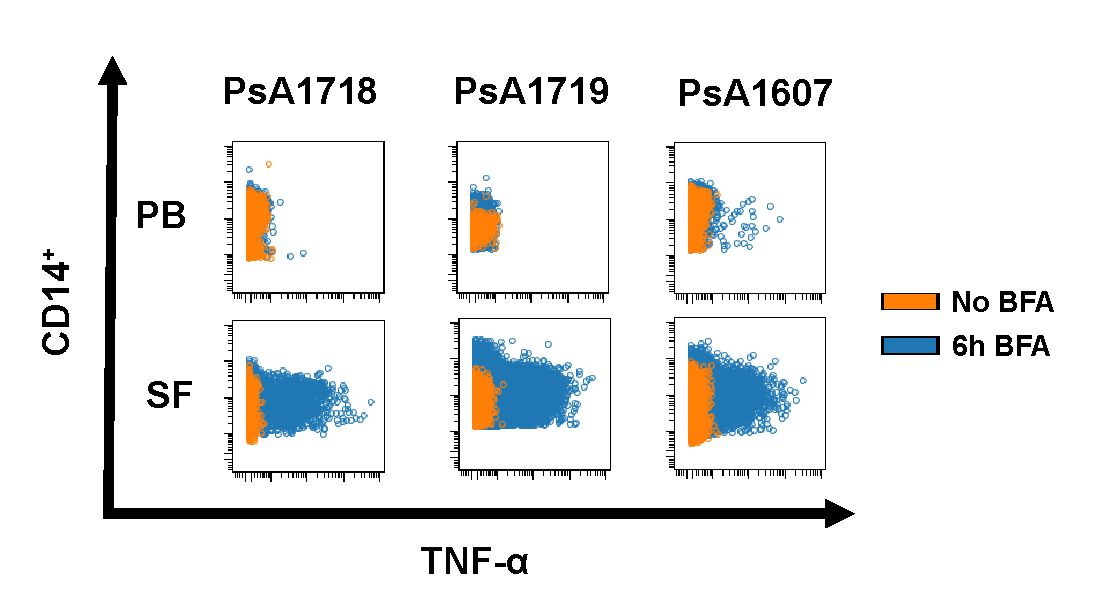
\includegraphics[width=\textwidth]{./Results3/pdfs/PSA_0h_6h_BFA_TNFa_mass_cytometry_PSA1718_PSA1719_PSA1607}
\caption{}
\end{subfigure}
~
\begin{subfigure}[b]{0.45\textwidth} 
%the [b] prevents offset in subcaptions
\centering
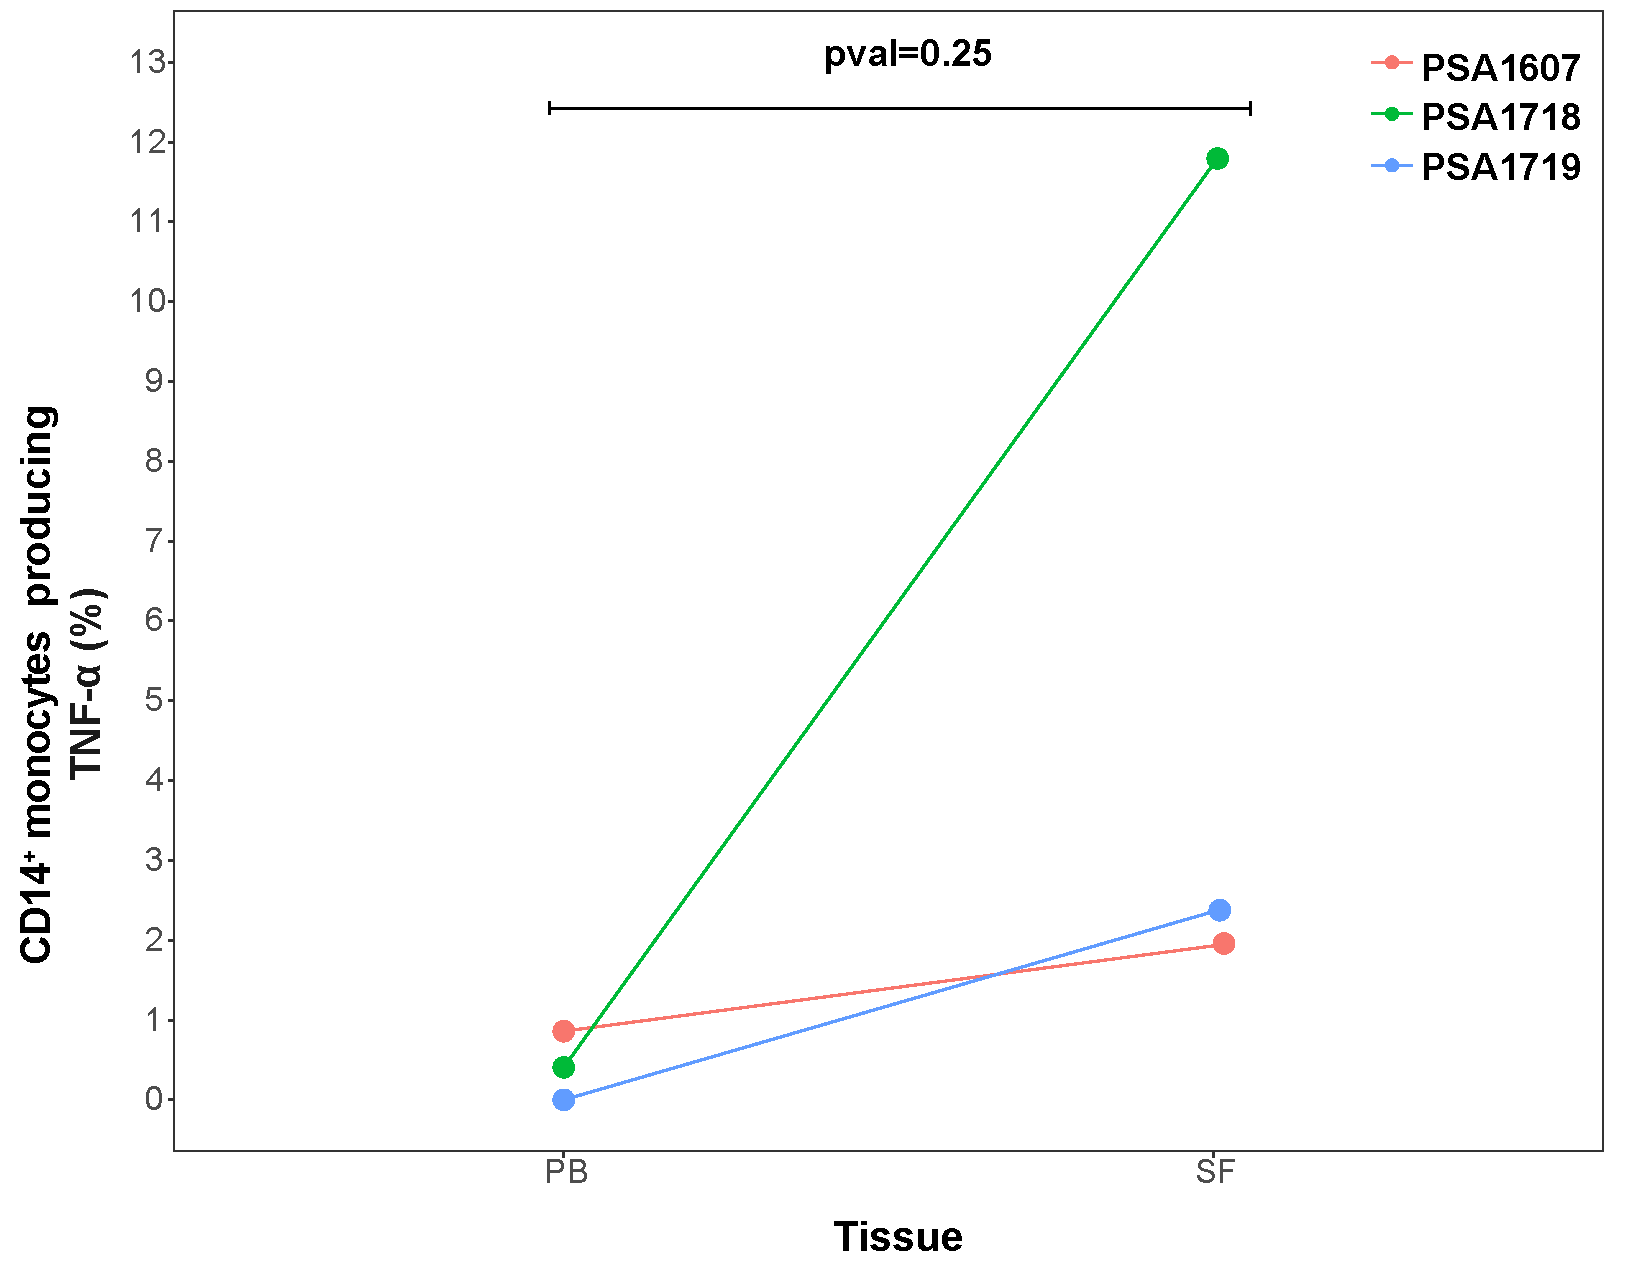
\includegraphics[width=\textwidth]{./Results3/pdfs/CyTOF_PSA1607_PSA1718_PSA1719_TNFa_percentage}
\caption{}
\end{subfigure}
\caption[Comparison of TNF-$\alpha$ expression in SF and PB CD14$^+$ monocytes before and after protein transport blockade with BFA using mass cytometry.]{\textbf{Comparison of TNF-$\alpha$ expression by SF and PB CD14$^+$ monocytes before and after protein transport blockade with BFA using mass cytometry.} a) For each of the three PsA patients, representation of CD14$^+$ (y-axis) versus TNF-$\alpha$ (x-axis) intensity of expression in matched SF and PB without protein transport blockade (blue dots) or after 6h treatment with BFA (orange dots). b) Percentage of CD14$^+$ monocytes producing TNF-$\alpha$ in SF and PB.For each tissue and sample shown in a, this percentage is calculated as the increment in cells producing TNF-$\alpha$ before and after protein transport blockade with BFA (6h minus 0h).}
\label{figure:PsA_monocytes_percentage_TNFa}
\end{figure}



In order to validate this observation and also assess other cytokines of interest, mass cytometry was conducted in PB and SF from another ten PsA patients. This validation cohort included the patients for which scRNA-seq data was presented in this chapter (Table \ref{tab:PSA_datasets_per_sample}). As previously, percentage of CD14$^+$ monocytes producing TNF-$\alpha$ , MCP-1 (protein product of \textit{CCL2} and osteopontin (protein product of \textit{SPP1}) was computed as the difference between percentage of cells producing each of the cytokines before and after BFA treatment. The percentage of CD14$^+$ monocytes producing TNF-$\alpha$ was greater in SF compared to PB (pval=0.048) (Figure \ref{figure:CyTOF_cytokines_validation_cohort} a), reinforcing the results from the previous cohort. Likewise, a larger percentage of CD14$^+$ monocytes producing osteopontin and MCP-1 (pval=0.001 and pval=0.003, respectively) were also observed in SF compared to PB (Figure \ref{figure:CyTOF_cytokines_validation_cohort} b and c), in line with the up-regulated expression of these two genes in SF compared to PB in bulk CD14$^+$ monocytes and in the CC-mixed scRNA-seq cluster. The percentage of cells producing cytokines in SF was particularly moderate for TNF-$\alpha$ and MCP-1, not exceeding of 1.8 and 3, respectively, for the majority of the PsA samples (Figure \ref{figure:CyTOF_cytokines_validation_cohort} a and c). However, one of the patients (PSA1505) appeared to have particularly higher percentage of SF CD14$^+$ monocytes producing all three cytokines when compared to the rest of the patients in the cohort. Although no justification was found to remove this sample, the statistical significance (pval$<$0.05) in the differences found between percentage of cell producing TNF-$\alpha$, MCP-1 and osteopontin in SF versus PB remained when repeating the analysis in absence of PSA1505.



\bigskip
\begin{figure}[H]
\centering
\begin{subfigure}[b]{0.40\textwidth}
\centering 
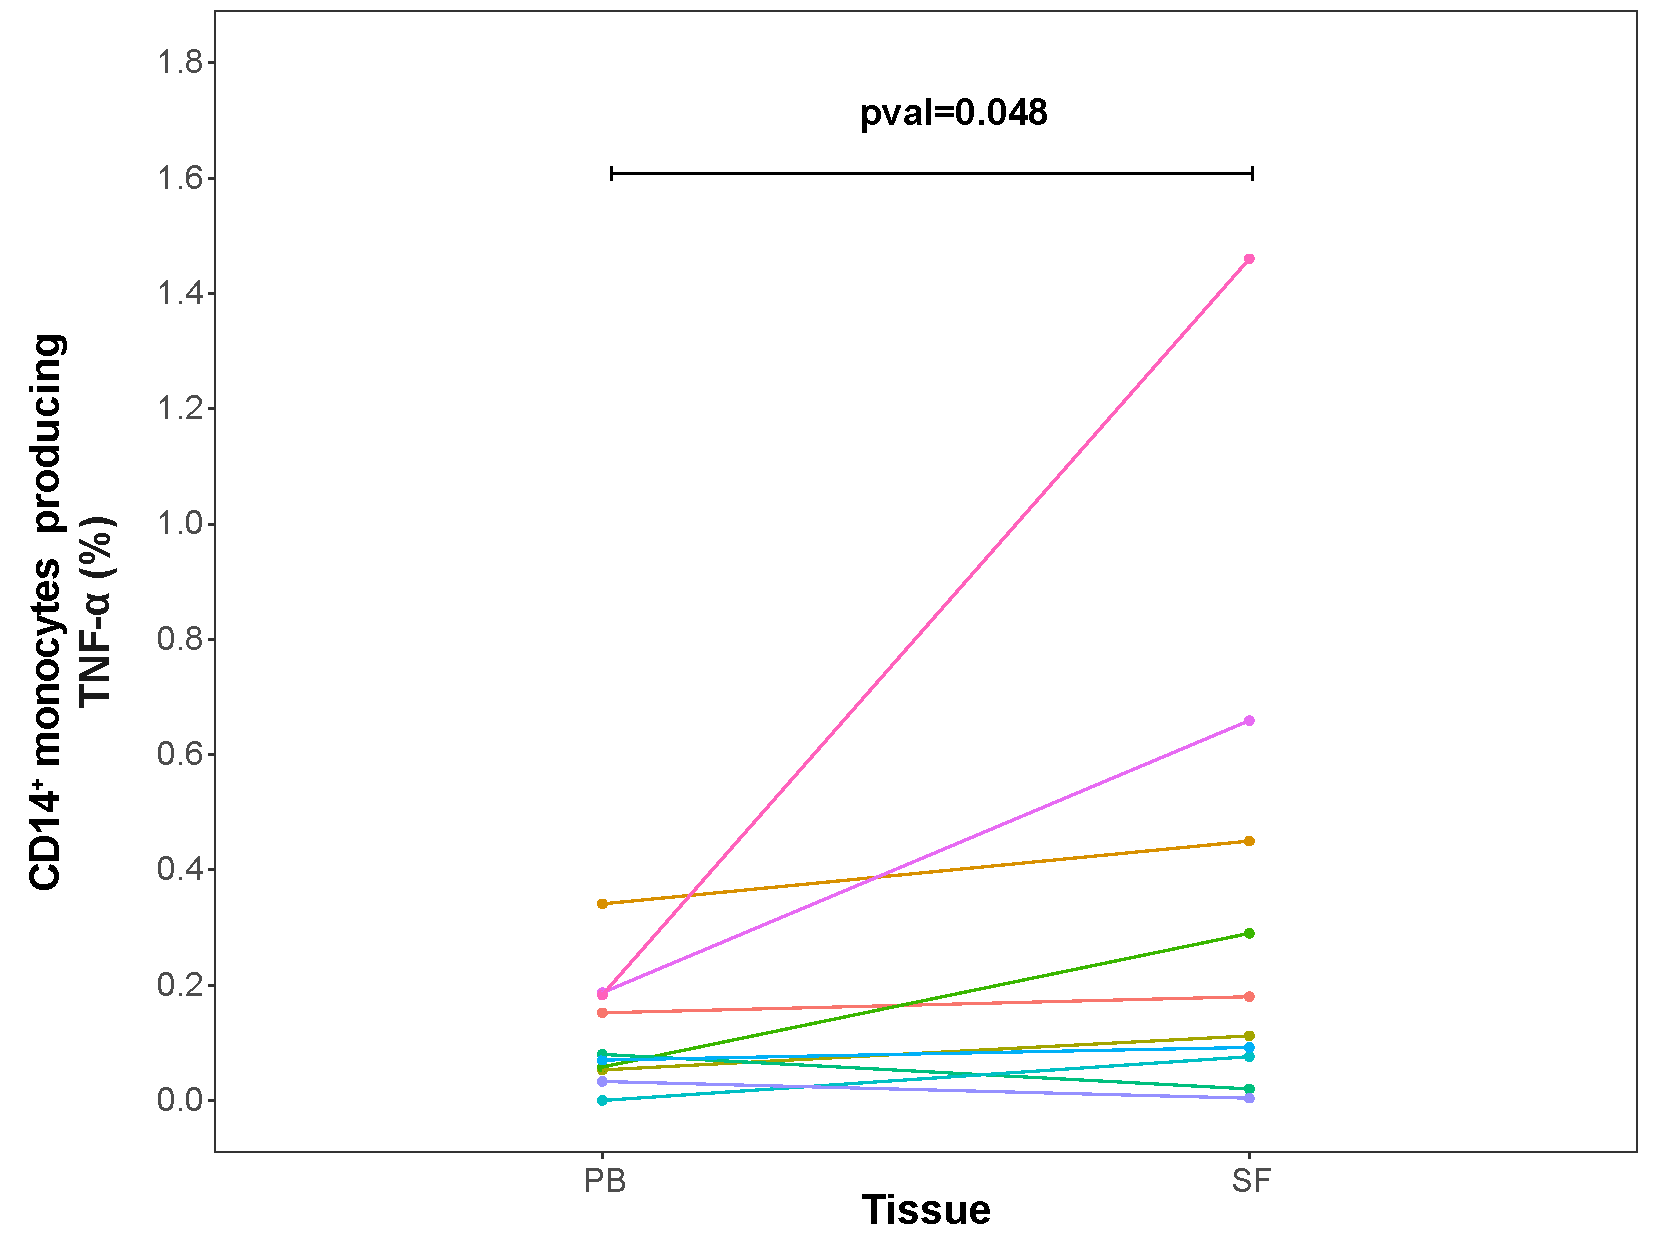
\includegraphics[width=\textwidth]{./Results3/pdfs/CyTOF_validation_cohort_TNFa_percentage}%
\caption{}
\end{subfigure}
~
\begin{subfigure}[b]{0.40\textwidth}
\centering 
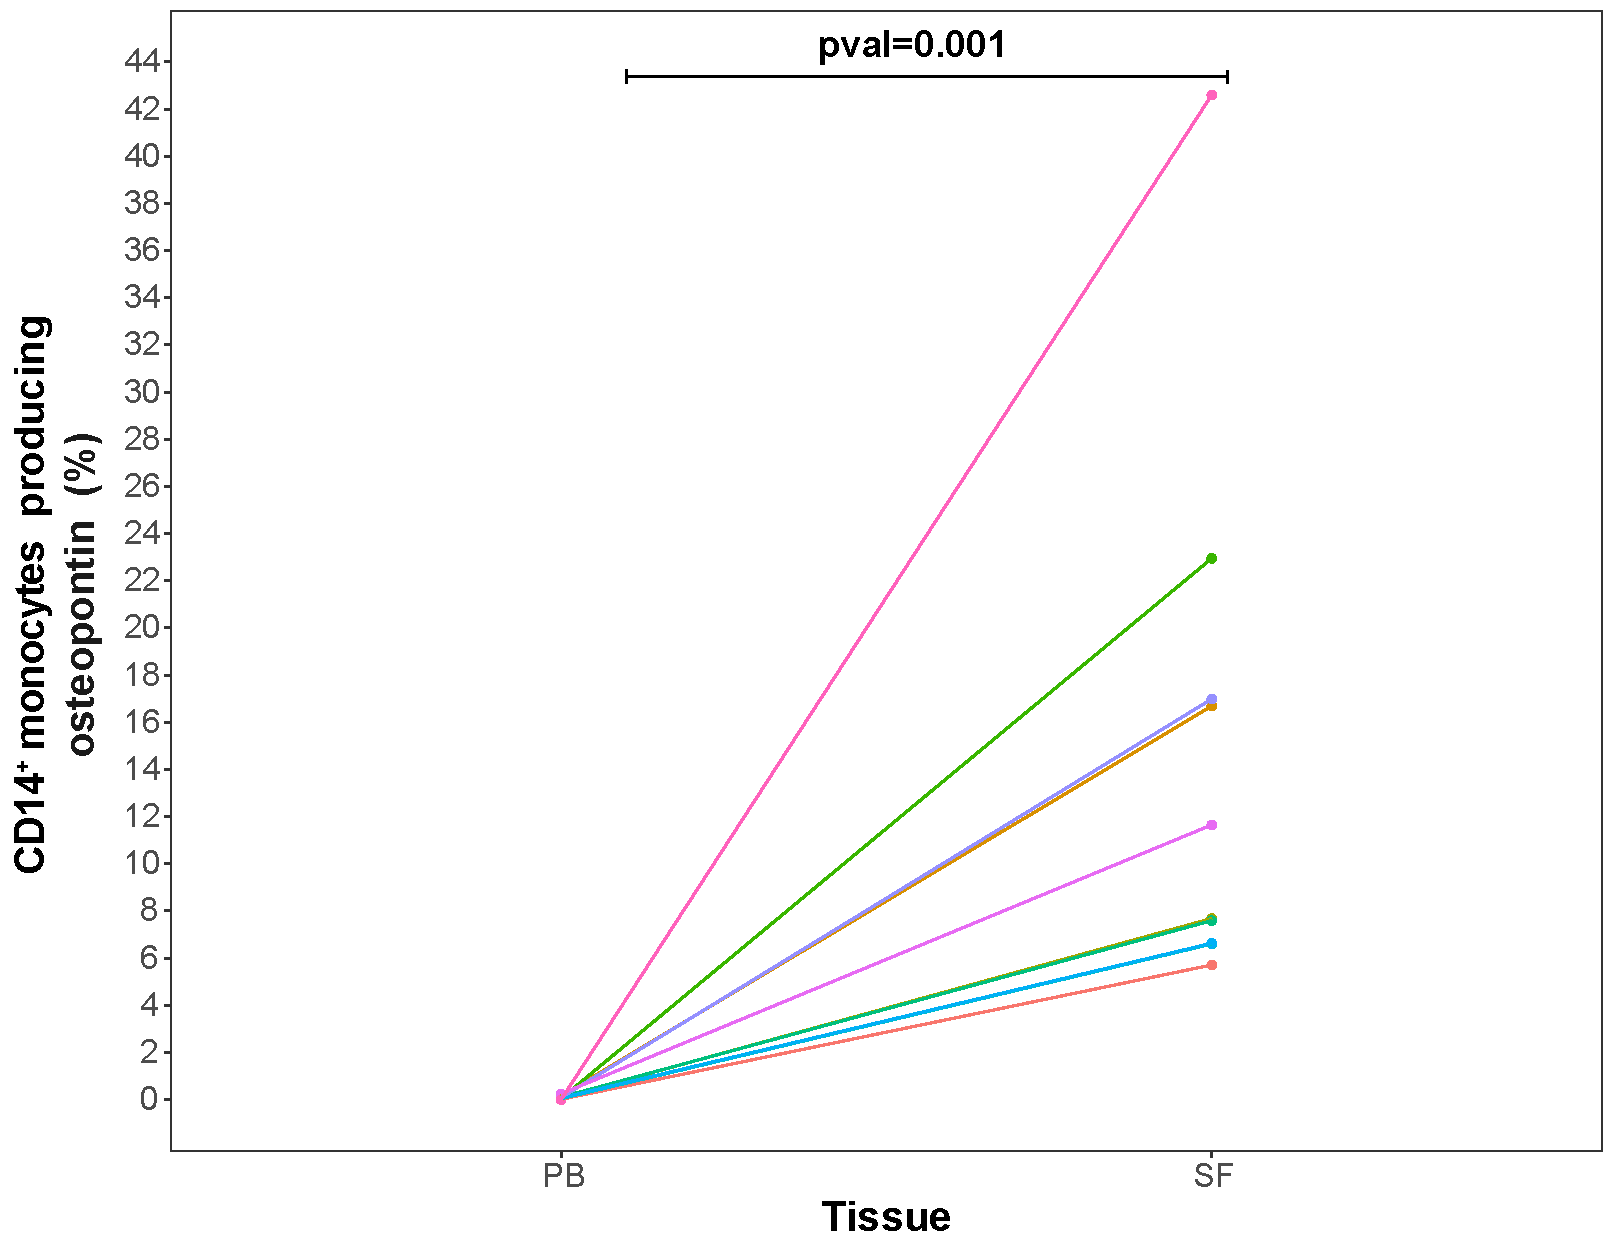
\includegraphics[width=\textwidth]{./Results3/pdfs/CyTOF_validation_cohort_osteopontin_percentage}
\caption{}
\end{subfigure}
~
\begin{subfigure}[b]{0.45\textwidth} 
%the [b] prevents offset in subcaptions
\centering
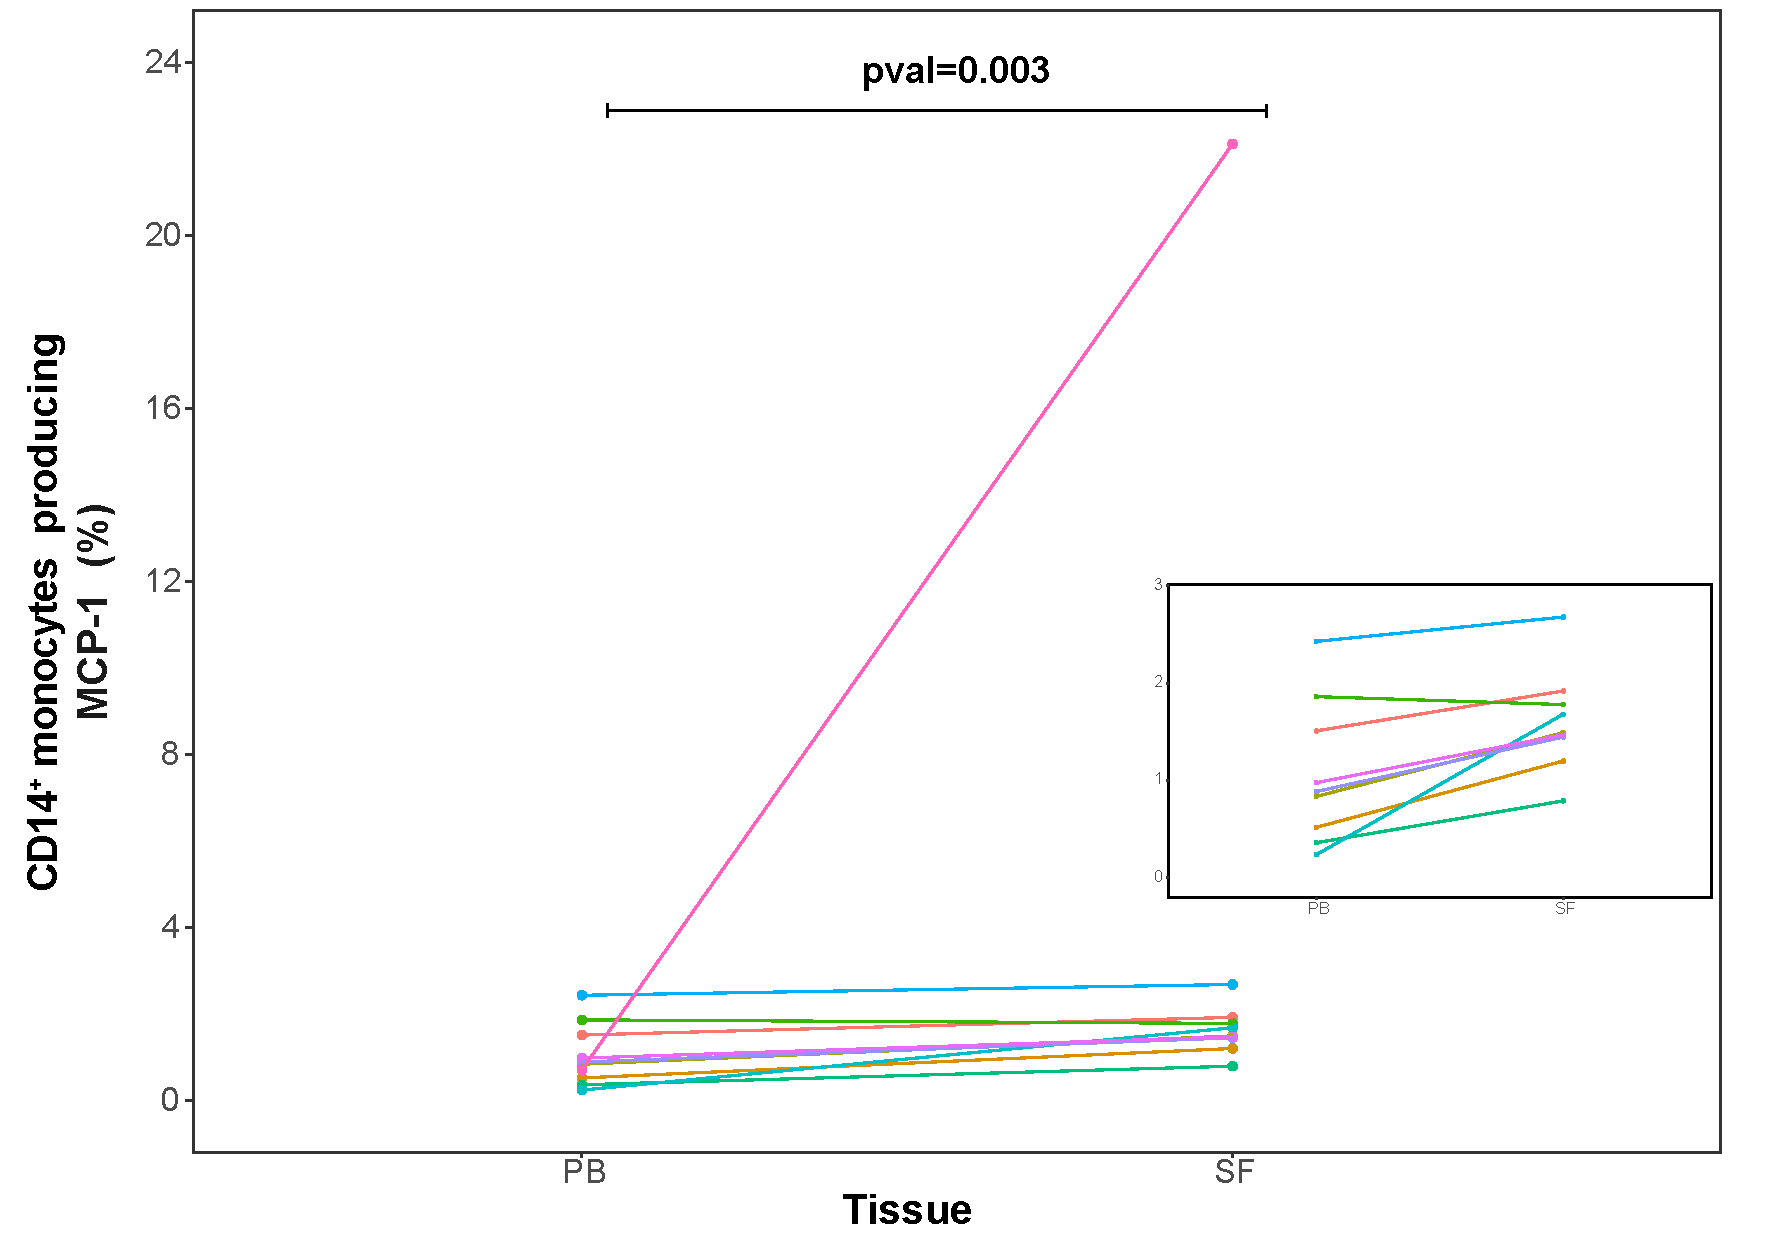
\includegraphics[width=\textwidth]{./Results3/pdfs/CyTOF_validation_cohort_CCL2_percentage}
\caption{}
\end{subfigure}
\caption[Percentage of CD14$^+$ monocytes producing TNF-$\alpha$, osteopontin and MCP-1 in SF and PB in a validation cohort of ten PsA samples.]{\textbf{Percentage of CD14$^+$ monocytes producing TNF-$\alpha$, osteopontin and MCP-1 in SF and PB in a validation cohort of ten PsA samples.} The percentage of CD14$^+$ monocytes producing a) TNF-$\alpha$, b) osteopontin and c) MCP-1 in SF and PB are shown for each of the ten samples in a PsA cohort used to validate cytokine production by mass cytometry. In each sample and tissue, this percentage is calculated as the increment in cells producing the relevant cytokine before and after protein transport blockade with BFA (6h minus 0h). In c), a zoom in for the percentage of CD14$^+$ monocytes producing MCP-1 in all patients minus PSA1505 is included for further detail on the differences across SF and PB for these samples.}
\label{figure:CyTOF_cytokines_validation_cohort}
\end{figure}


\subsubsection{\textit{CCL2}-\textit{CCR2} signalling: an example of multi-omics correlation}

The differences in percentage of CD14$^+$ monocytes producing MCP-1 between SF and PB represent an example of a putative correlation between changes observed in the chromatin accessibility landscape, bulk and scRNA-seq expression and protein production. Differential chromatin accessibility analysis between SF and PB identified a statistically significant cell type-specific SF open DAR upstream \textit{CCL2} gene (Figure \ref{figure:PsA_10X_qPCR_ATAC_CD14_CCL2}). This SF open DAR region is annotated as enhancer according to Epigenome Roadmap chromatin segmentation and overlaps a eRNA reported by FANTOM5 in CD14$^+$ monocytes. The expression of \textit{CCL2} was shown to be significantly modulated (pval$<$0.05 and mean FC$>$1.5) between SF and PB by qPCR in CD14$^+$ monocytes only, whereas no significant changes were observed for mCD4$^+$ and mCD8$^+$ in this data from the same patients (Figure \ref{figure:PSA_PCR_array_vulcano_plots} a, b, c and Table \ref{tab:PSA_gene_expression_ATAC_overlap}). Up-regulation of \textit{CCL2} was not found in PB CD14$^+$ monocytes compared to PsA patients and healthy controls, being defined as one of the tissue-specific genes in the previous analysis (Figure \ref{figure:figure:PSA_PCR_array_HC_FC_correlation} a).  Furthermore, \textit{CCL2} was also identified by scRNA-seq as one of the up-regulated genes in the CC-mixed cluster (Figure \ref{figure:PsA_scRNAseq_vulcano_plots_mixed_and_IL7R_clusters} a and \ref{figure:PsA_scRNAseq_qPCR_ATAC_correlation} a and b). Expression of \textit{CCR2}, the receptor for the chemokine MCP-1 (protein product of \textit{CCL2}), appeared up-regulated by qPCR in SF mCD4$^+$ and mCD8$^+$ cells in the same individuals, which could suggest increased chemotaxis driven by CD14$^+$ monocytes and leading to T cell infiltration in the synovium. Interestingly, in this data no significant up-regulation of \textit{CCR2} was observed in PsA PB when compared to healthy controls in any of the three cell types.   


\bigskip
\begin{figure}[H]
\centering
\begin{subfigure}[b]{0.55\textwidth}
\centering 
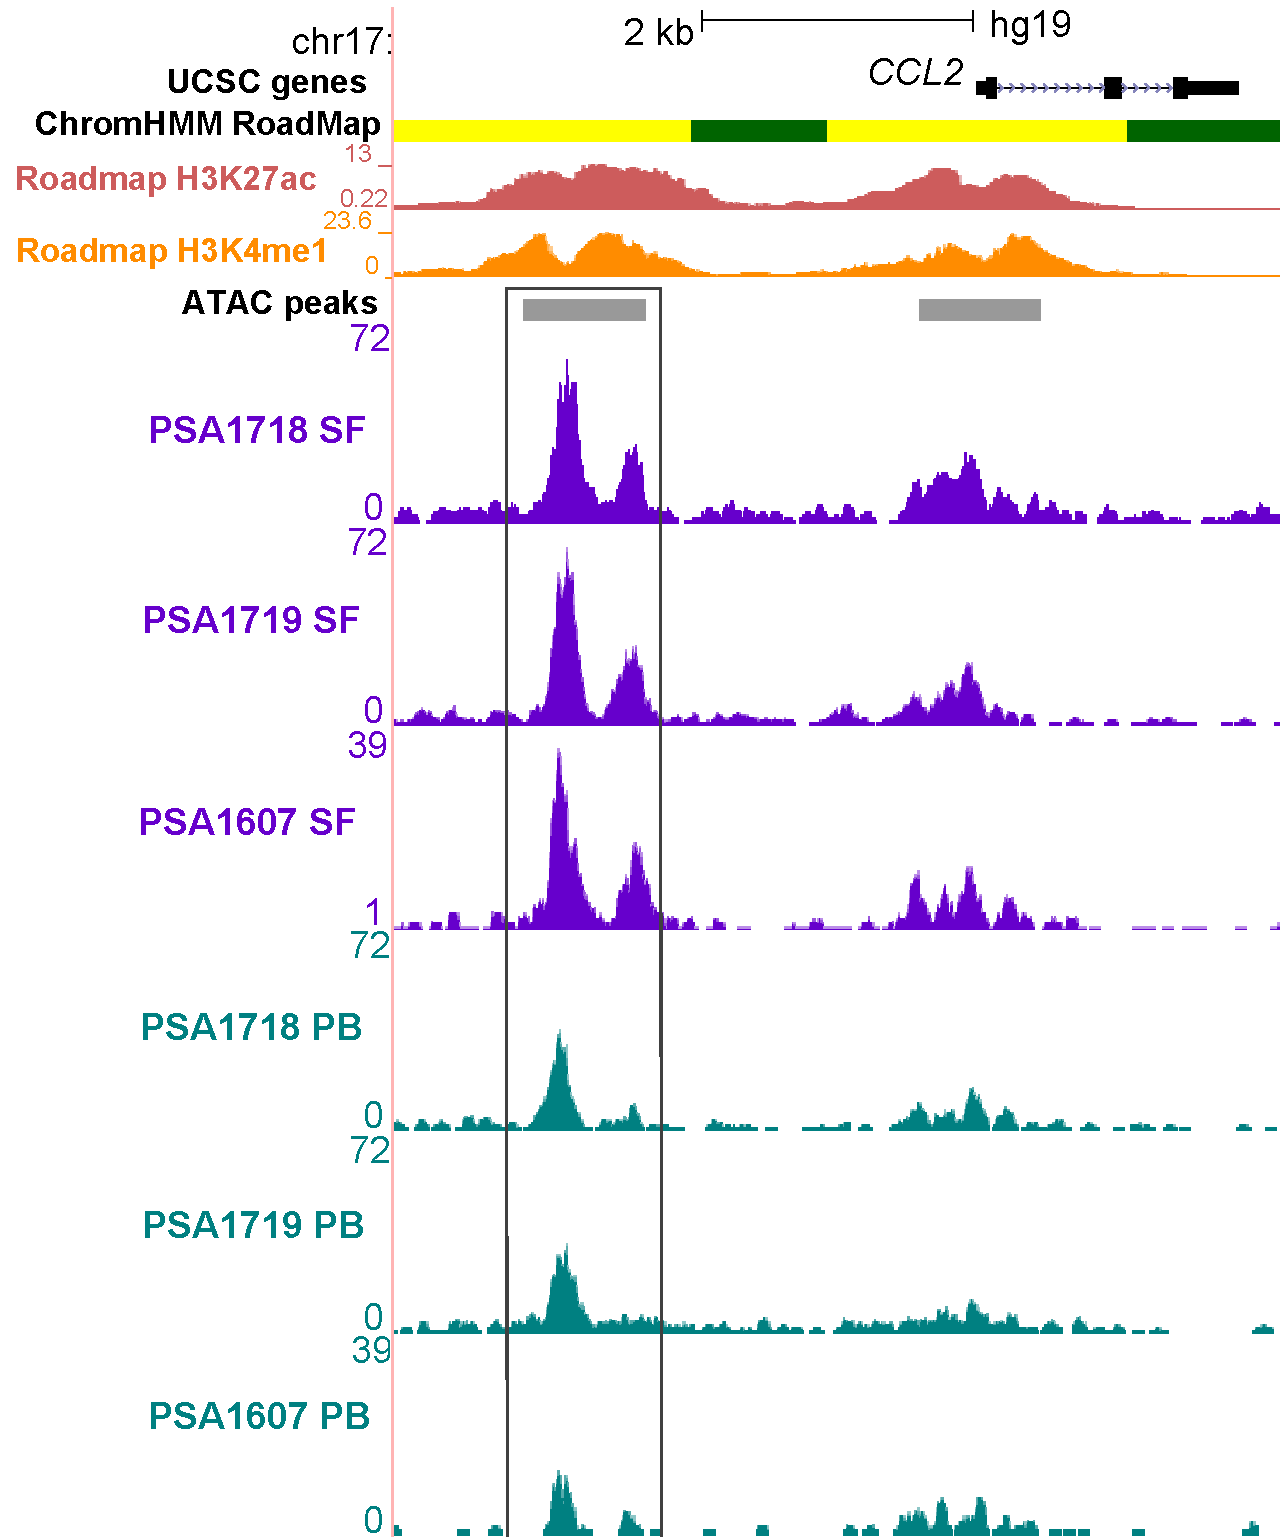
\includegraphics[width=\textwidth]{./Results3/pdfs/ATAC_PSA_CD14_UCSC_CCL2_track}
\caption{}
\end{subfigure}
\caption[Chromatin landscape in CD14$^+$ monocytes upstream the differentially expressed gene \textit{CCL2}.]{\textbf{Chromatin landscape in CD14$^+$ monocytes upstream the differentially expressed gene \textit{CCL2}.} UCSC Genome Browser view illustrating the normalised ATAC read density (y-axis) for two ATAC peaks at the promoter and upstream the \textit{CCL2} gene (x-axis) in SF and PB CD14$^+$ monocytes from three PsA patients. The ATAC peak upstream \textit{CCL2} (black rectangle) appeared as a significant DAR (FDR$<$0.01 and FC$>$1.5) in the differential analysis, being more more accessible in SF when compared to PB. Tracks are colour-coded by tissue (SF=purple and PB=turquoise). Additional epigenetic tracks of PB isolated CD14$^+$ monocytes from the Epigenome Roadmap, including chromatin segmentation map and the enhancer marks H3Kme1 and H3K27ac, are also included.}
\label{figure:PsA_10X_qPCR_ATAC_CD14_CCL2}
\end{figure}



In addition to the mass cytometry data, collaborators in Basel have performed measurements of cytokine levels in PB and SF from same ten patients in the validation cohort. High levels of MCP-1 (approximately 1,000 pg/mL) were also reported in SF whereas this cytokine was below the lower detection level in the assay in plasma, supporting additional evidence of \textit{CCL2} up-regulated expression at the protein level (Figure \ref{figure:ELISA_SF_PsA}). Overall, the data here presented suggests a tissue and cell type specific dysregulation of \textit{CCL2} expression in the CC-mixed CD14$^+$ monocytes cluster that may be related to alterations in the chromatin accessibility of an enhancer in the proximity to this gene.



\subsection{Prioritisation and interpretation of PsA GWAS SNPs}

The generation of epigenetic and expression data from different cell types isolated from SF and PB aims to contribute to the general understanding of disease pathophysiology and differences between affected and non-affected tissue. Furthermore, overlapping this data derived from clinical samples with fine-mapped credible sets of SNPs may be more informative for refining the number of putative functional causal variants in non-coding or intergenic GWAS associations, compared to the only integration of epigenetic data from cell lines or healthy controls.


\subsubsection{Bayesian fine-mapping using genotyping data}

In order to further refine the PsA Immunochip GWAS signals identified by Bowes and colleagues, Bayesian fine-mapping was conducted using genotype data from 1,103 patients and 8,900 controls, which corresponds to the PsA Immunochip UK cohort from Bowes \textit{et al.}, 2015. Bowes and colleagues performed fine-mapping for some of the loci and reported the number of independent signals for each locus as well as the number of SNPs in the credible set \parencite{Bowes2015} accounting for 99\% of the association in that regions. Nevertheless, \textit{de novo} fine-mapping was conducted here to obtain the exact identity of the SNPs in the credible set and integrate them with the chromatin accessibility data generated in this chapter. 

Fine-mapping was performed in 36 loci reported in Bowes \textit{et al.}, all showing at least nominal significance in their GWAS study. Out of the 36 loci, 22 showed log$^{_10}ABF$ under 3 (cut-off used in \parencite{Bunt2015}) for the lead SNP in the fine-mapping association analysis (Table \ref{tab:PsA_loci_no_fine_mapping}). The majority corresponded to GWAS signals with the lowest significance for the lead SNP (pval$>10^{-4}$) in Bowes \textit{et al.} study, such as \textit{RSPH3/TAGAP} or \textit{ELMO1} (Table \ref{tab:PsA_loci_no_fine_mapping}) and they were not fine-mapped either by Bowes \textit{et al.},2015. Some of those regions with pval$<10^{-4}$, for example \textit{DDX58}, were also discarded by Bowes and colleagues for fine-mapping based on marker density being lower than 100 SNPs. 
 

\begin{landscape}
\begin{center}
%\begin{longtable}[ht]{p{.25\textheight} p{.40\textheight} p{.25\textheight} p{.60\textheight}}
\begin{longtable}[ht]{c c c c c c c c c c}
\caption[Summary table of the PsA GWAS loci presenting log${_10}ABF>3$ for the fine-mapping lead SNP.]{\textbf{Summary table of the PsA GWAS loci presenting -log${_10}$ABF$>$3 for the fine-mapping lead SNP.} For 12 PsA loci log${_10}ABF$ of the fine-mapping lead SNP was 3 or greater. In 4 of those loci ($^{\ast}$) the fine-mapping lead SNP was in low LD (r${^2}<0.5$) with the PsA GWAS SNP and/or did not contain it in the credible set. FM=fine-mapping; MAF= minor allele frequency; OR=odds ratio; ABF=approximate Bayes factor; PP=posterior probability.}
\label{tab:PsA_fine_mapping_summary} \\
\toprule
\textbf{chr} & \textbf{Closer} & \textbf{FM} & \textbf{MAF} & \textbf{OR} & \textbf{log${_10}ABF$} & \textbf{PP} & \textbf{90\% credible} &\textbf{Bowes FM} & \textbf{Bowes 90\%}\\
    & \textbf{gene} & \textbf{lead SNP} & & \textbf{FM} & \textbf{FM lead SNP} &  & \textbf{set} &\textbf{lead SNP} & \textbf{credible set} \\
\midrule
\midrule
2	 &\textit{IFIH1}	       & rs13406089$^{\ast}$	&0.33	&0.78	&4.58	&0.48	&2	&rs35667974	&4 \\
5	 &\textit{IL12B/ADRA1B}  & rs2546890	&0.48	&0.76	&6.53	&0.6	&23	&rs4921482	&3 \\
5	 &\textit{IL13}	         &rs2069616$^{\ast}$	  &0.44	&1.25	&5.16	&0.05	&55	&NA	 &NA \\
1	 &\textit{IL23R}	       &rs12044149	&0.25	&1.41	&9.83	&0.14	&29	&rs12044149	&34 \\
1	 &\textit{IL28RA/GRHL3}  &rs2135755$^{\ast}$	&0.50	&1.20	&3.06	&0.03	&49	&NA	&NA \\
19 &\textit{ILF3}	         &rs11085727$^{\ast}$	&0.30	&0.79	&3.83	&0.22	&35	&NA	&NA \\
17 &\textit{PTRF/STAT3}    &rs730086$^{\ast}$ &0.34 &0.81 &3.39 &0.39 &400	&NA	&NA \\
1	 & \textit{RUNX3}	       & rs6600250	&0.50	&1.20	&3.07	&0.03	&48	&rs7523412	&52 \\
12 &\textit{STAT2/IL23A}	 &rs12368739	&0.06	&1.70	&4.04	&0.02	&110 &	rs2020854	&121 \\
6	 & \textit{TRAF3IP2}	   &rs33980500	&0.07	&1.71	&8.26	&0.87	&2	&rs33980500	&7 \\
19 &	\textit{TYK2}	       &rs11085727	&0.30	&0.79	&3.83	&0.21	&32	&rs34725611	&5 \\
5	 & \textit{CSF2/P4HA2}	 &rs11242104  &0.48 &1.24 &5.31 &0.07 &58	&rs715285 &35 \\
\bottomrule
%\medskip
\end{longtable}
\end{center}
\end{landscape}


Amongst the loci that failed to be fine-mapped in this analysis, 4 (\textit{B3GNT2}, \textit{NOS2A}, \textit{REL} and \textit{TNIP1}) had been successfully fine-mapped by Bowes and colleagues (Table \ref{tab:PsA_loci_no_fine_mapping}). This is consistent with the dependence of fine-mapping success on sample size \parencite{Bunt2015} and highlighted the reduced power of the analysis presented here, limited by a smaller sample size (only UK cohort as previously mentioned).


Of the 12 loci passing the log${_10}ABF\geq3$ cut-off, 5 showed fine-mapping lead SNPs in very low LD (r${^2}<0.5$) with the PsA GWAS lead SNP and/or did not contain the GWAS lead SNP in the credible set (Table \ref{tab:PsA_fine_mapping_summary} labelled with $\ast$). In some cases this was the result of the association analysis identifying spurious signals or signals from other loci nearby. For example, the association analysis performed for the fine-mapping of the \textit{IL13} locus was confounded by the \textit{TYK2} signal. The additional 7 signals successfully fine-mapped in this study contained the lead GWAS SNP and Bowes and colleagues fine-mapped lead SNPs in the credible sets and ranged between 2 and 110 SNPs in the 90\% credible set (Table \ref{tab:PsA_fine_mapping_summary}). Moreover, two of those loci,\textit{IL23R} and \textit{TRAF3IP2}, presented the same fine-mapping lead SNPs as the reported by Bowes \textit{et al.},2015. Regarding additional independent signals, a secondary signal reported by Bowes and colleagues in the \textit{IL12B} locus was also identified here by step-wise conditional analysis. 


\subsubsection{Integrating fine-mapped SNPs and chromatin accessibility from PsA samples}
The union of the 90\% credible sets for the 7 successfully fine-mapped loci comprised a total of 292 unique SNPs. These SNPs were used to perform overlap with the significant (FDR$<$0.01 and FC$>$1.5) DARs identified between SF and PB in CD14$^+$ monocytes, mCD4$^+$, mCD8$^+$ and NK cells. Unfortunately, none of the 292 SNPs were contained by a DAR in any of these cell types. Additional overlap was performed between these SNPs and the accessible chromatin regions (consensus peaks without filtering based on the differential analysis) in each of the four cell types assayed by ATAC. The largest number of SNPs (17) was found to overlap accessible chromatin in CD14$^+$ monocytes, followed by mCD8$^+$, mCD4$^+$ and NK cells (Table \ref{tab:PSA_fine_mapping_ATAC_overlap}). The 43 unique SNPs from the 90\% credible set overlapping ATAC accessible chromatin were distributed across the \textit{CSF2} (8), \textit{IL12B} (3), \textit{IL23R} (4), \textit{RUNX3} (6), \textit{STAT2} (14), \textit{TRAF3IP2} (1) and \textit{TYK2} (7) loci. A number of these SNPs were found to only overlap accessible chromatin in one particular cell type. Interestingly, for the \textit{TRAF3IP2} locus, which was fine-mapped with the greatest resolution, none of the two SNPs of the 90\% credible set overlapped accessible chromatin in any of the four studied cell types.


\begin{table}[htbp]
%\setlength{\tabcolsep}{20pt} only to stretch the columns if you want
%\renewcommand{\arraystretch}{1.5}
\centering
\begin{tabular}{@{} c c c}
\toprule
\textbf{ATAC cell type} & \textbf{90\% credible set}   &  \textbf{Cell type specific}  \\
\textbf{master list}    & \textbf{overlapping SNPs}    &   \textbf{overlap}   \\
									      &	\textbf{(number)}				     &                            \\
\midrule
\midrule
 CD14$^+$ monocytes    & 32                            &  \textit{STAT2} (5), \textit{TYK2}(2)\\ 
                       &                               &  \textit{RUNX3}(1),\\
											 &                               &  \textit{TRAF3IP2}(1) \\
 mCD4$^+$              & 29                            &  \textit{CSF2}(1), \textit{IL23R}(1) \\
 mCD8$^+$              & 28                            &  \textit{RUNX3} (1)        \\
 NK                    & 19                            &  \textit{TYK2} (1)       \\
\bottomrule
\end{tabular}
\medskip %gap
\caption[PsA fine-mapped SNPs from the 90\% credible sets overlapping accessible chromatin identified by ATAC in four cell types.]{\textbf{PsA fine-mapped SNPs from the 90\% credible sets overlapping accessible chromatin identified by ATAC in four cell types.} The number of SNPs in the 90\% credible set union from the eight fine-mapped loci overlapping each cell type ATAC master list are reported. Furthermore, the number of SNPs only found to overlap open chromatin in one cell type are indicated together with the locus in which the SNP was fine-mapped.}
\label{tab:PSA_fine_mapping_ATAC_overlap}
\end{table}


SNPs from the fine-mapping credible set were significantly enriched in ATAC peaks when compared to all other GWAS Catalog SNPs and SNPs in LD (r$^2$=8) in all four cell types (Fisher exact test: CD14$^+$ monocytes pval=7.12x$10^{-8}$, mCD4$^+$ pval=1.69x$10^{-10}$, mCD8$^+$ pval=6.40x$10^{-9}$ and NK pval=1.86x$10^{-5}$). Notably, the GWAS Catalog SNPs overlapping ATAC accessible regions were significantly enriched (FDR$<$0.001) for particular terms from the Experimental Factor Ontology (EFO) (Figure \ref{figure:GWAS_traits_enriched_for_ATAC_ML}). The EFO is a hierarchical tree-like ontology where each term represents a (disease) trait or group of related (disease) traits with which disease-risk SNPs may be annotated (Figure \ref{figure:GWAS_traits_enriched_for_ATAC_ML}). Enrichment for general terms (towards the root of the tree) including autoimmune diseases, rheumatic diseases and skin diseases were found across all four cell types. Disease-specific terms (amongst the branches of the tree) related to these general terms, such as CD and IBD, were also found to be enriched for SNPs overlapping ATAC in all four cell types. Conversely, other "branches" from more general terms, including psoriasis and MS, presented significant enrichment (FDR$<$0.001) only in CD14$^+$ monocytes and mCD4$^+$ cells, respectively. Overall, this reinforced the specificity of the overlap between GWAS Catalog genetic variants not included in the fine-mapping credible set with accessible chromatin across the immune cell types investigated in this chapter.




%This enrichment of GWAS Catalogue SNPs overlapping mCD4$^+$ ATAC peks for MS is consistent with the key role of this cell type in the pathophysiology \parencite{Bielekova2000}.   



\begin{figure}[htbp]
\centering
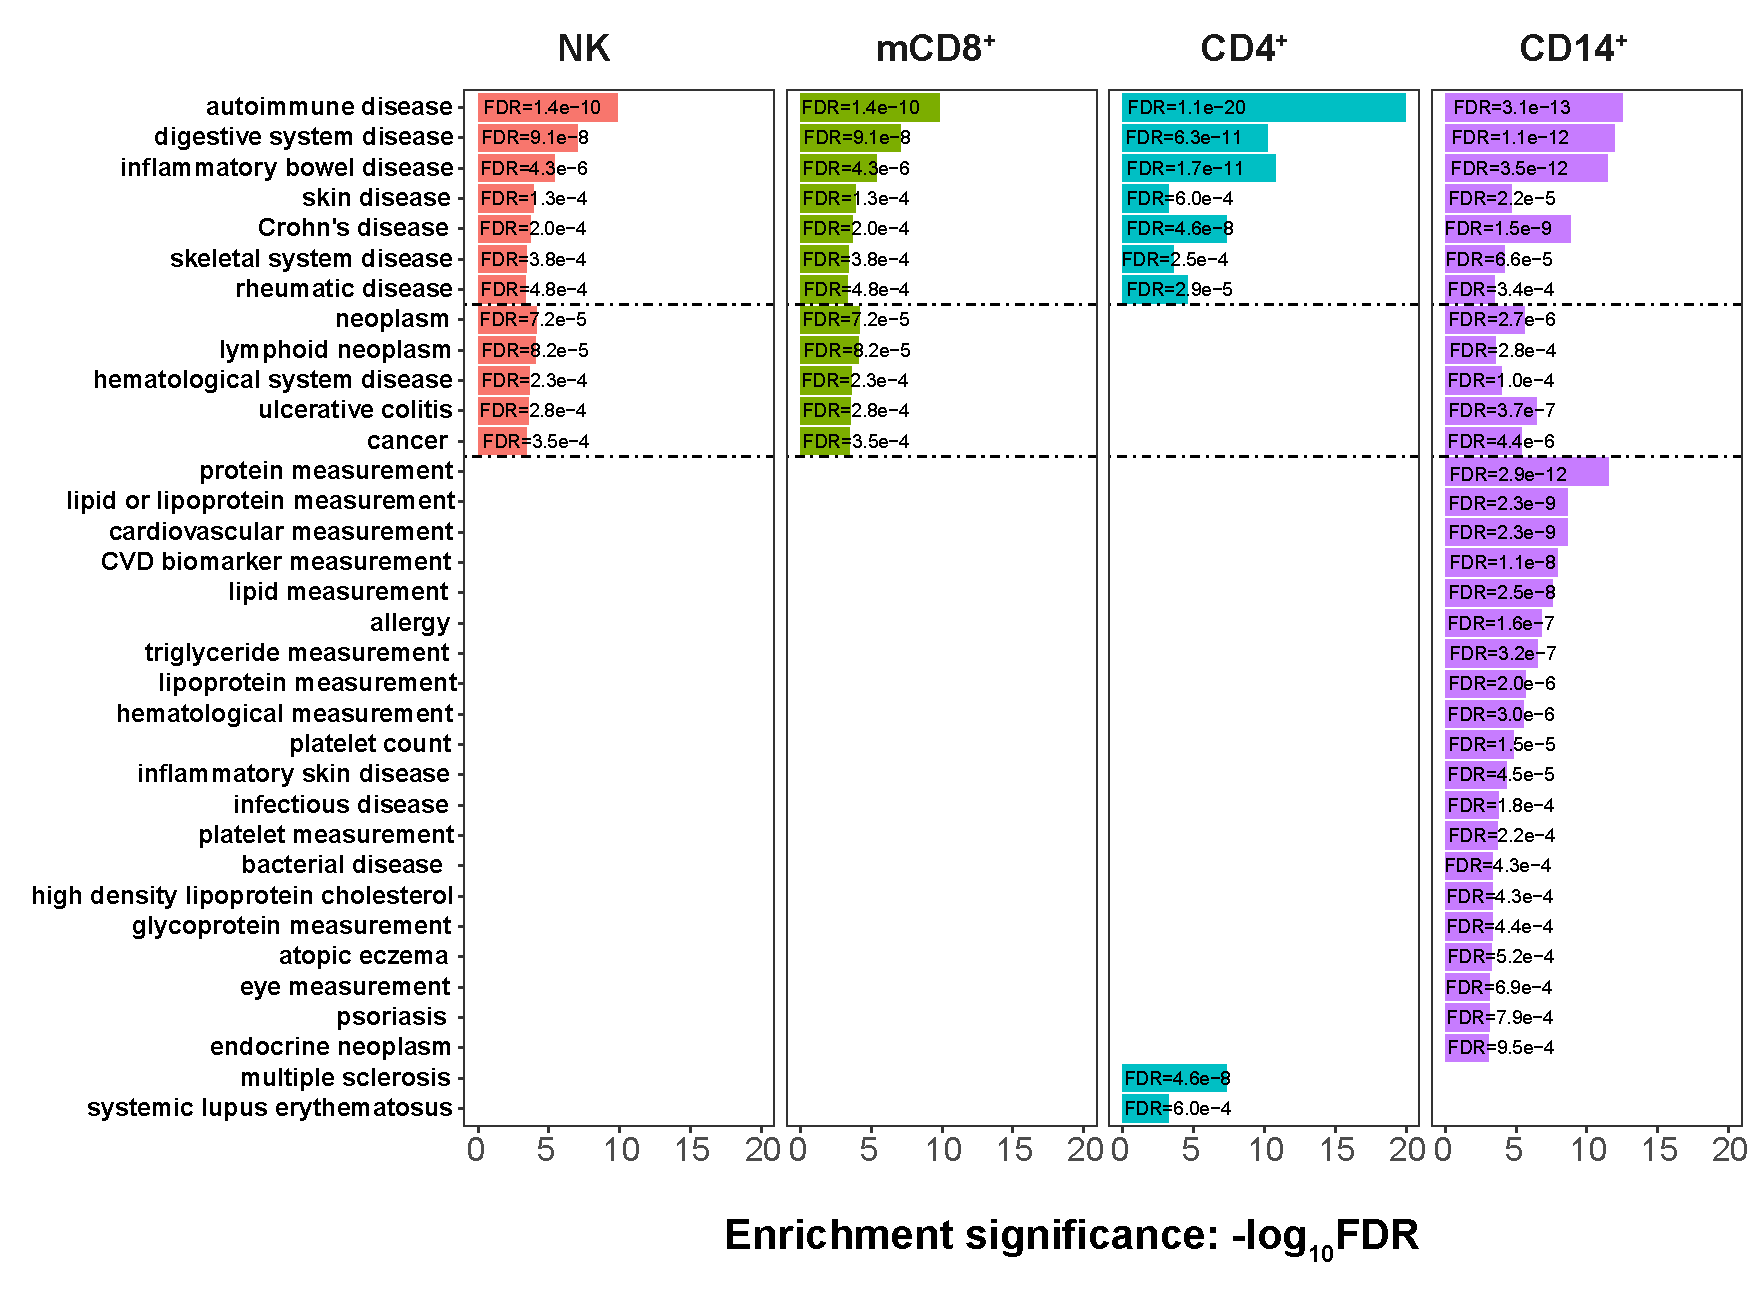
\includegraphics[width=0.75\textwidth]{./Results3/pdfs/Enrichment_for_FM_GWAS_cat_SNPs_overlapping_ATAC}
\caption[Experimental Factor Ontology terms enriched in GWAS Catalog SNPs overlapping ATAC regions in four cell types.]{\textbf{Experimental Ontology Factor terms enriched for GWAS Catalog SNPs overlapping ATAC regions in four cell types.} Each term annotates a set of risk SNPs associated with a disease trait or a group of related disease traits. Enrichment analysis was performed using as input data the GWAS Catalog SNPs overlapping ATAC accessible chromatin regions. A minimum of ten SNPs overlap and FDR$<$0.001 was required for enrichment to be considered significant.}
\label{figure:GWAS_traits_enriched_for_ATAC_ML}
\end{figure}



\subsubsection{Further investigating the PsA-specific 5q31 locus}
Following fine-mapping, integration of in-house ATAC and additional functional data with the 90\% set of SNPs was conducted to further investigate the 5q31 locus, harbouring the only PsA GWAS association not shared with psoriasis. Out of the 58 SNPs in the 90\% credible set, only 8 overlapped ATAC accessible chromatin in at least one of the four cell types included in this study (Figure \ref{figure:5q31_fine_mapping_SNPs_epigenetic_track} top panel). Amongst those SNPs were three (rs10065787, rs27437 and rs7721882) of the four variants highlighted by Bowes and colleagues as the most functionally relevant according to ENCODE epigenetics data. 


\begin{table}[htbp]
%\setlength{\tabcolsep}{20pt} only to stretch the columns if you want
%\renewcommand{\arraystretch}{1.5}
\centering
\begin{tabular}{@{} c c c}
\toprule
\textbf{SNP} & \textbf{Cell type ATAC}   & \textbf{Top eGene , cell type } \\
             & \textbf{overlap}          & \textbf{and condition}  \\
\midrule
\midrule
rs10065787   & CD14$^+$, mCD4$^+$        & \textit{P4HA2} (monocytes LPS2, LPS24, IFN-$\gamma$) \\
             &                           &  \textit{SLC22A5} (monocytes UT) \\
rs11242104   & All                       &     NA        \\ 
rs11242105   & All                       &     NA   \\
rs2069803    & All                       & \textit{SLC22A5} (CD4$^+$$^{(\ast)}$, CD8$^+$) \\   
rs27437      & CD14$^+$, mCD4$^+$        & \textit{SLC22A5} (CD4$^+$, CD8$^+$) \\ 
rs4705908    & All                       & \textit{SLC22A5} (CD4$^+$$^{(\ast)}$, CD8$^+$) \\
rs2089855    & All                  & \textit{P4HA2} (monocytes LPS2, LPS24, IFN-$\gamma$,) \\
             &                           & \textit{SLC22A5} (monocytes UT, IFN-$\gamma$,\\
						 &                           & CD4$^+$$^{(\ast})$, CD8$^+$$^{(\ast)}$)  \\
rs7721882    & mCD4$^+$                  & \textit{SLC22A5} (CD4$^+$$^{(\ast)}$, CD8$^+$) \\									
\bottomrule
\end{tabular}
\medskip %gap
\caption[Publicly available \textit{cis}-eQTL datasets reporting an effect for the PsA 5q31 GWAS locus fine-mapped SNPs (90\% credible set) overlapping ATAC accessible regions.]{\textbf{Publicly available and unpublished \textit{cis}-eQTL datasets reporting an effect for the PsA 5q31 GWAS locus fine-mapped SNPs (90\% credible set) overlapping ATAC accessible regions.} For each of the SNPs, the cell type for the ATAC overlap, the gene which expression is reported to be regulated by the SNP (eGene) and the cell type where the eQTL study was conducted are specified.The eQTLs datasets included in the analysis were monocytes (UT, LPS 2h, LPS 24h, IFN-$\gamma$) \parencite{Fairfax2014}, B cells \parencite{Fairfax2012}, NK untreated \parencite{Naranbhai2015}, neutrophils untreated (unpublished), tCD4$^+$ and tCD8$^+$ \parencite{Kasela2017} and whole blood \parencite{Jansen2017}. $^{(\ast)}$ for eQTLs extremely significant (FDR$<$2.2x10$^{-308}$).}
\label{tab:5q31_SNPs_ATAC_eQTL}
\end{table}

The SNP rs10065787, highlighted by Bowes \textit{et al.} for overlapping with ENCODE clusters of occupancy for TFs relevant in CD4$^+$ and CD8$^+$ biology, presented accessible chromatin in CD14$^+$ monocytes and mCD4$^+$ cells, showing also moderate enrichment for the the enhancer histone mark H3K4me1 in mCD4$^+$ (Figure \ref{figure:5q31_fine_mapping_SNPs_epigenetic_track} right hand side panel red line). Similarly, the nearby SNP rs27437 overlapped an ATAC peak in CD14$^+$ monocytes and mCD4$^+$ and the same TFBS site cluster as rs10065787 (Table \ref{tab:5q31_SNPs_ATAC_eQTL} and Figure \ref{figure:5q31_fine_mapping_SNPs_epigenetic_track} right hand side panel green line). rs10065787 appeared to be part of an eQTL signal for \textit{SLC22A5} and \textit{P4HA2} expression in unstimulated and stimulated monocytes (LPS2, LPS24, IFN-$\gamma$), respectively (Table \ref{tab:5q31_SNPs_ATAC_eQTL}). However, no \textit{cis} eQTL for tCD4$^+$ was reported for this SNP in the Kasela and colleagues dataset (Table \ref{tab:5q31_SNPs_ATAC_eQTL}). In contrast, rs27437 was part of a \textit{cis}-eQTL in tCD4$^+$ and tCD8$^+$ for \textit{SLC22A5}, the same eGene reported by Bowes and colleagues in their pilot eQTL study. Chromatin conformation data using promoter capture-HiC \parencite{Javierre2016} in unstimulated monocytes does not clearly reveal interaction for rs10065787 with the promoter of \textit{P4HA2} or \textit{SLC22A5}. Conversely, rs27437 is relatively close to the bait in the \textit{IL3} promoter, which interacts with \textit{SLC22A5}, potentially bringing this SNP in proximity with the promoter of \textit{SLC22A5}.  



Other SNPs such as rs2089855 also appeared in an eQTL signal for \textit{P4HA2} and \textit{SLC22A5} in untreated and stimulated monocytes, and were associated with \textit{SLC22A5} expression in tCD4$^+$ cells (Table \ref{tab:5q31_SNPs_ATAC_eQTL}). This SNP is proximal to rs11955347, which in Bowes \textit{et al.} presented the most significant correlation with expression of \textit{SLC22A5} in tCD4$^+$ and tCD8$^+$, and has also shown to be within the \textit{cis}-eQTL signal for \textit{SLC22A5} expression in unstimulated and IFN-$\gamma$ stimulated monocytes and for \textit{P4HA2} in monocytes stimulated with LPS (2 and 24h) \parencite{Fairfax2014}. The effect of rs11955347 genotype in modulation of \textit{SLC22A5} expression was also confirmed in the larger data set of Kasela \textit{et al.} in both tCD4$^+$ and tCD8$^+$ cells. These observations suggest a role for the 5q31 PsA-specific GWAS association in regulating expression of \textit{P4HA2} and \textit{SLC22A5} not only in T cells but also in monocytes under different conditions.

\begin{figure}[htbp]
\centering
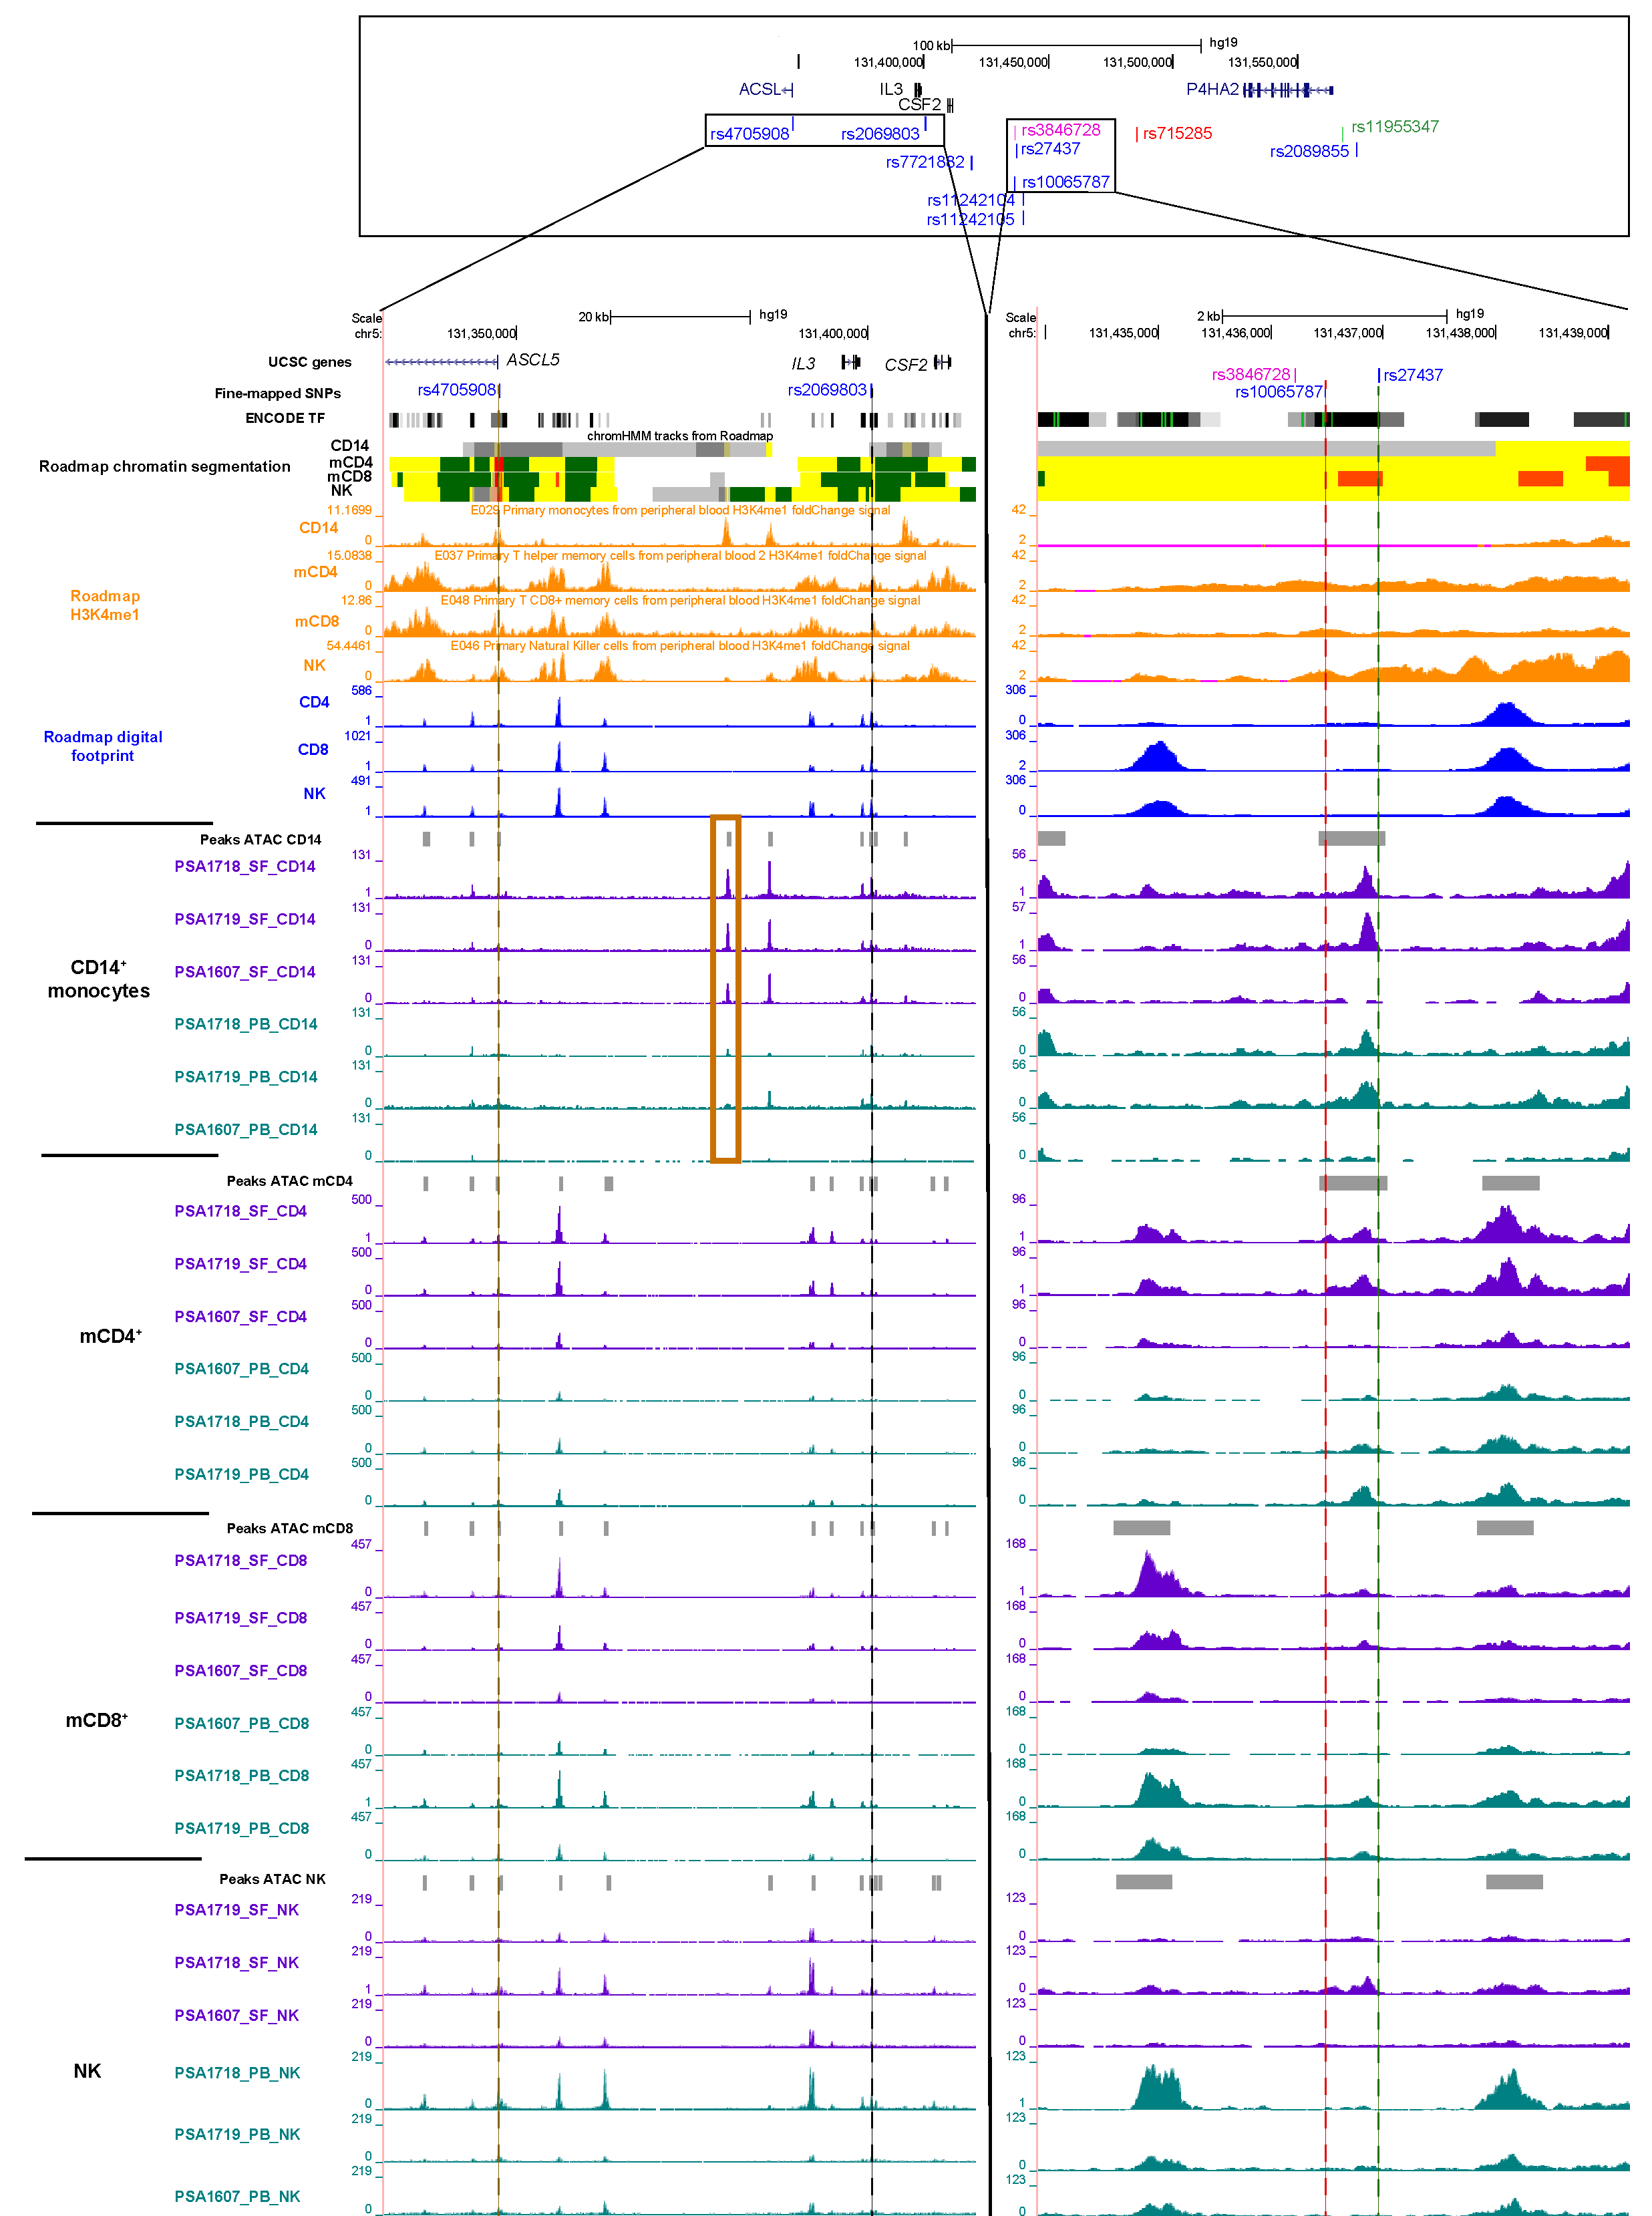
\includegraphics[width=0.7\textwidth]{./Results3/pdfs/UCSC_chr5q31_credible_set_all_cell_types_multipanel_final}
\caption[Epigenetic landscape at the genomic location of fine-mapped SNPs for the 5q31 PsA GWAS signal.]{\textbf{Epigenetic landscape at the genomic location of fine-mapped SNPs for the 5q31 PsA GWAS signal.} The top panel shows the genomic location of the six SNPs in the 5q31 fine-mapping 90\% credible set overlapping PsA ATAC accessible regions in at least one of the four cell types (in blue). The schema also includes the location of relevant SNPs for the 5q31 PsA-specific GWAS region from the Bowes \textit{et al.}, study, including the GWAS lead SNP (in red), the eQTL SNP showing the best correlation with the GWAS lead SNP (in green) and one SNPs from the credible set overlapping several ENCODE annotation features with no overlap for my PsA ATAC data (in purple). The left and right hand side panels are the UCSC visualisation of the epigenetic landscape for rs4705908 and rs2069803 (left brown and black lines, respectively) and rs1006587 and rs27437 (right, red and green lines, respectively), which represent four of the most relevant fine-mapped SNPs at the 5q31 in terms of overlap with PsA ATAC data signal for eQTLs. For each panel, all the ATAC tracks from three PsA patients and four cell types isolated from SF and PB are included. ATAC tracks are colour-coded by tissue (SF=purple and PB=turquoise). Additionally, publicly available epigenetic data (H3K4me1, chromatin segmentation maps, digital footprint and ENCODE cluster for TF binding) generated in the same cell types as the in-house ATAC are included. The yellow box highlights a DAR found in CD14$^+$ monocytes near rs2069803 and rs4705908. H3K4me1 relative fold-enrichment signal and ATAC normalised counts within each cell type are shown (y-axis).}
\label{figure:STAT2_fine_mapping_SNPs_epigenetic_track}
\end{figure}


Another two relevant SNPs from the 90\% credible set reported here were rs2069803 and rs4705908, both overlapping ATAC peaks in all four cell types (Figure \ref{figure:5q31_fine_mapping_SNPs_epigenetic_track} left hand side panel black and brown lines, respectively). rs4705908 is located upstream from the promoter of the \textit{ACSL6} gene in a region showing H3K4me1 enrichment, supporting a regulatory role. Notably, rs4705908 maps to a CTCF binding site reported in GM12878 and LCLs cell lines. Likewise, rs2069803 also overlaps moderate H3K4me1 signal in mCD4$^+$, mCD8$^+$ and NK cells (Figure \ref{figure:5q31_fine_mapping_SNPs_epigenetic_track} left hand side panel). The region has also been annotated as an enhancer and weakly transcribed in mCD4$^+$, mCD8$^+$ and NK cells by the Epigenome Roadmap chromatin segmentation maps (yellow and light green in \ref{figure:5q31_fine_mapping_SNPs_epigenetic_track} left hand side panel). Although accessible chromatin has been identified at rs2069803 and rs4705908 for all cell types, \textit{cis}-eQTL for these two SNPs have only been reported in CD4$^+$ or CD8$^+$, with the genotypes of both SNPs correlating with regulation of \textit{SLC22A5} expression with extremely high significance in tCD4$^+$ cells (Table \ref{tab:5q31_SNPs_ATAC_eQTL}). Promoter capture Hi-C data in na\'{i}ve and total CD4$^+$ CD8$^+$ cells revealed interaction of the \textit{IL3} promoter bait containing rs2069803  with the promoter of \textit{SLC22A5}. Interestingly, rs4705908 also appeared within the bait of the \textit{ACSL6} promoter interacting with the \textit{IL3} promoter bait, which also includes the previously mentioned rs2069803 variant. Overall, promoter-capture HiC data revealed potential physical interactions between rs27437, rs2069803 and rs4705908 in CD4$^+$ and CD8$^+$ cells with potential functional relevance in regulation of \textit{SLC22A5} expression.

Lastly, rs7721882 was the only SNP showing a very significant eQTL effect in tCD4$^+$ for \textit{SLC22A5} expression and overlapping with a putative mCD4$^+$ cell type specific ATAC peak (Table \ref{tab:5q31_SNPs_ATAC_eQTL}). However, additional replicates and greater sequencing depth would be required in order to confirm the robustness of this peak as well as the cell type specificity in mCD4$^+$ cells.  


In addition to epigenetic evidence, further investigation of the suitability of \textit{SLC22A5} and \textit{P4HA2}, two of the genes showing eQTLs for some of the SNPs in the 5q31 credible set, as drug targets for PsA was investigated. Dr Hai Fang has developed an algorithm named Priority Index (Pi) based on random forest to levearage genetic information in the prioritisation of putative drug targets for particular complex diseases. Interestingly, \textit{SLC22A5} appeared as the third gene in the psoriasis rank supported as eGene in several immune cell eQTLs studies, annotation by the disease ontology with related inflammatory disease terms (including CD, IBD and RA, amongs others) as well as prediction for high druggability based on protein structure data (\url{http://galahad.well.ox.ac.uk:3010/pidb/discovery/PSO/SLC22A5#bookmark_details_genomic}). In contrast, \textit{P4HA2} appeared 4,172 in the rank for psoriasis, not being such a suitable putative drug target in this disease. 

%Promoter capture-HiC from Javierre \textit{et al.} in tCD4$^+$ and tCD8$^+$ cells revealed  direct rs743564 interaction with \textit{P4HA2} and proximity to a downstream fragment that presents frequent interaction with \textit{SLC22A5} promoter in both cell types. Interestingly, rs1469149, another SNP from the credible overlapping a mCD4$^+$-specific ATAC peak (Table \ref{tab:5q31_SNPs_ATAC_eQTL}) is found to be in the same bait as rs743564 interacting with \textit{SLC22A5} promoter. The SNP rs1469149 also presents a extremely significant signal for a tCD4$^+$ eQTL regulating \textit{SLC22A5} expression and less significant eQTLs in stimulated monocytes (Table \ref{tab:5q31_SNPs_ATAC_eQTL}). 


%In contrast, rs10065787 was found to be a \textit{cis}-eQTL in stimulated monocytes (LPS 2h, LPS 24h and IFN-$\gamma$) regulating \textit{P4HA2} expression (Table \ref{tab:5q31_SNPs_ATAC_eQTL}). The nearby SNP rs27437 overlapped an ATAC peak in CD14$^+$ monocytes and mCD4$^+$ and the same TFBS site cluster than rs10065787 (Table \ref{tab:5q31_SNPs_ATAC_eQTL} and Figure \ref{figure:5q31_fine_mapping_SNPs_epigenetic_track} right hand side panel green line). The enhancer histone mark H3K4me1 was absent in CD14$^+$ monocytes and only moderate in mCD4$^+$ (Figure \ref{figure:5q31_fine_mapping_SNPs_epigenetic_track} right hand side panel). Interestingly, \textit{cis}-eQTL were only reported for tCD4$^+$ and tCD8$^+$ associated to modulation of expression for \textit{SLC22A5}, the same eGene reported by Bowes and colleagues in their pilot eQTL study. Nevertheless, chromatin conformation data has not revealed any interaction for rs10065787 with the promoter of \textit{P4HA2}. Conversely, rs27437 is relatively close to the bait in \textit{IL3} which interacts with \textit{SLC22A5}, potentially bringing this SNP in proximity with the promoter of the eQTL eGene repoted in tCD4$^+$ and tCD8$^+$ Kasela's dataset. 
%
%Another two relevant SNPs from the 90\% credible set here reported were rs2069803 and rs4705908, both overlapping ATAC peaks in all four cell types (Figure \ref{figure:5q31_fine_mapping_SNPs_epigenetic_track} left hand side panel black and brown lines, respectively). Rs4705908 is located upstream the promoter of \textit{ACSL6} gene and is overlapping a region enriched for H3K4me1, supporting a regulatory role for that region. Notably, rs4705908 is mapping to a CTCF binding site reported in GM12878 and LCLs cell lines. Likewise, rs2069803 is also overlapping open chromatin and moderate H3K4me1 signal in mCD4$^+$, mCD8$^+$ and NK cells (Figure \ref{figure:5q31_fine_mapping_SNPs_epigenetic_track} left hand side panel). The region has also been annotated as enhancer and weakly transcribed in mCD4$^+$, mCD8$^+$ and NK cells by the Epigenome Roadmap chromatin segmentation maps (yellow and light green in \ref{figure:5q31_fine_mapping_SNPs_epigenetic_track} left hand side panel). Although accessible chromatin has been identified at rs2069803 and rs4705908 for all cell types, \textit{cis}-eQTL for these two SNPs have only been reported in CD4$^+$ or CD8$^+$, with the genotypes of both SNPs correlating with regulation of \textit{SLC22A5} expression, with extremely high significance in tCD4$^+$ cells (Table \ref{tab:5q31_SNPs_ATAC_eQTL}). Promoter capture Hi-C data in na\'{i}ve and total CD4$^+$ CD8$^+$ cells revealed interaction of the \textit{IL3} promoter bait containing rs2069803  with the promoter of \textit{SLC22A5}. Interestingly, rs4705908 appeared also within the bait of the \textit{ACSL6} promoter interacting with the \textit{IL3} promoter bait, which also includes the rs2069803 as previously mentioned \parencite{Javierre2016}. Overall, promoter-capture HiC data revealed potential physical interaction between rs27437, rs2069803 and rs4705908 in CD4$^+$ and CD8$^8$ cells with potential functional relevance in gene expression regulation of \textit{SLC22A5}.

%The PsA GWAS lead SNP rs715285 was also contained in the credible set but was mapped to a region of closed chromatin and depleted signals for H3K4me1 and digital footprint in all four cell types. Likewise, the aforementioned eQTL SNP rs11955347 from Bowes study showing the strongest correlation with \textit{SLC22A5} expression also appeared in a region depleted for open chromatin and activating epigenetic marks, suggesting that one or more of the previously highlighted SNPs from the 90\% credible set may be responsible for the effect on gene expression regulation detected by eQTL studies for \textit{P4HA2} and \textit{SLC22A5} expression. 



%\subsubsection{Overview of fine-mapping and epigenetic data integration for other loci}
%In addition to the 5q31 locus (\textit{CSF2/P4HA2}), another seven loci were successfully fine-mapped in this analysis. As previously mentioned, integration of epigenetic data and fine-mapping credible set of SNPs is particularly relevant when trying to identify putative causal SNPs for GWAS signals lying in non-coding regions. An example amongst the fine-mapped loci is \textit{IL12B}, for which a PsA GWAS lead SNP as well as the fine-mapped lead SNP found in this analysis were located upstream of the gene. Out of the 52 SNPs identified in the 90\% credible set only four appeared to overlap accessible chromatin in at least two of the cell types analysed by ATAC in PsA samples and they were not in LD with common non-synonymous SNPs in \textit{IL12B}. The PsA GWAS SNP rs4921482 (primary signal in Bowes and colleagues) overlapped a strong ATAC peak in all cell types as well as H3K4me1 enhancer marks. However, none of the four SNPs in the credible set overlapping ATAC peaks was found within a \textit{cis}-eQTL signal in any of the explored datasets.
%
%
%For another two loci fine-mapped in this analysis, \textit{STAT2/IL23A} and \textit{TRAF3IP2}, previous evidence for high LD between the psoriasis GWAS signal and missense coding variants in \textit{STAT2} and \textit{TRAF3IP2}, respectively, had been reported \parencite{Tsoi2012}. For the psoriasis GWAS \textit{STAT2} signal, Tsoi \textit{et al.}, 2012 highlighted a missense mutation (rs2066807) with a predicted highly damaging effect in this gene that is in very high LD with the GWAS lead SNP (Figure \ref{figure:STAT2_fine_mapping_SNPs_epigenetic_track} purple line). This SNP also appeared in the 90\% credible set of SNPs in this analysis. Although rs2066807 did not overlap ATAC accessible chromatin in any of the four cell types, it mapped to a RUNX3 and CTCF binding site in the cell lines GM12878 and K562. SNPs from the credible set located in the vicinity of this missense variant were found within eQTL signals of interest. For example, rs2371494 overlapped an ATAC peak in all four cell types (Figure \ref{figure:STAT2_fine_mapping_SNPs_epigenetic_track} black line) and presented a highly significant eQTL effect for \textit{STAT2} expression in unstimulated monocytes (FDR=7.54x10$^{-31}$) and to a lesser significance under IFN-$\gamma$ stimulation (FDR=9.94x10$^{-6}$). Fairfax and colleagues reported a negative effect for the major allele (G) of rs2371494 and also for the PsA GWAS lead SNP rs2020854 (T) (LD r$^2$=0.79) in both conditions, indicating increased expression of \textit{STAT2} for the GWAS risk allele. Interestingly, the nearby SNP rs57870697 which is in very high LD (r${^2}\geq$0.79) with rs2371494, overlapped a CD14$^+$ monocyte specific ATAC peaks in SF and PB (Figure \ref{figure:STAT2_fine_mapping_SNPs_epigenetic_track} red line) but no eQTL for any gene has been reported at the location of this SNP.
%
%Lastly, fine-mapping for the \textit{RUNX3/SYF3} locus identified 48 SNPs in the credible set, of which six overlapped ATAC peaks in CD14$^+$ monocytes and mCD8$^+$ cells. One mapped to a discrete mCD8$^+$ specific peak at the edge of a CTCF and RELA binding site in GM12878. Nevertheless, no eQTL has been reported for any of the six SNPs overlapping ATAC in any of the datasets.



%%Fine-mapping of the PsA GWAS signal in chr2 nearby \textit{STAT2} and \textit{IL23A} genes yielded 110 SNPs in the credible set of SNPs, very similar to the size of the credible set reported by Bowes and colleagues for this locus. Out of the 110 SNPs, 8 were found to overlap with an ATAC peak in at least one cell type. Amongt those 8 SNPs, rs2371494 located upstream the \textit{IL23A} and \textit{STAT2} genes, appeared to be of particular interest. Rs2371494 overlapped an ATAC peak in all four cell types (Figure \ref{figure:STAT2_fine_mapping_SNPs_epigenetic_track} black line) and presented a highly significant eQTL effect for \textit{STAT2} expression in unstimulated monocytes (FDR=7.54x10${^-31}$) and to a lesser significance under IFN-$\gamma$ stimulation (FDR=9.94x10${^-6}$). Fairfax and colleagues reported a negative effect for the major allele (G) of rs2371494 and also for the PsA GWAS lead SNP rs2020854 (T) (LD r$^2$=0.79) in both conditions, indicating increased expression of \textit{STAT2} for the GWAS risk allele. Additional eQTLs with lower significance for other eGenes were also reported for rs2371494 and other SNPs in the credible set. 
%
%%Interestingly, rs35157967 and rs57870697, two SNPs of the credible set in the vicinity and in very high LD (r${^2}\geq$0.79) with rs2371494, were overlapping SF and PB CD14$^+$ monocyte specific ATAC peaks (Figure \ref{figure:STAT2_fine_mapping_SNPs_epigenetic_track} red and green lines). Rs35157967 is located upstream \textit{IL23A} and \textit{STAT2} genes and rs57870697 is found within a \textit{STAT2} intron. Both SNPs were also mapping to H3K4me1 in CD14$^+$ monocytes and ENCODE clusters for TFs. Notably, rs35157967 is overlapping binding sites for for STAT2 and IRF1 in K562 cell line. The fact that no eQTL for \textit{STAT2} gene has been reported for none of those two SNPs in the same conditions as for rs2371494 may be consequence of those two SNPs not having been imputed in Fairfax \textit{et al.} analysis. Hypothetical existence of an eQTL signal for \textit{STAT2} could suggest a functional role of rs35157967 and/or rs57870697 in the regulation of \textit{STAT2} expression in homeostasis and under IFN-$\gamma$ stimulation in CD14$^+$ monocytes. Nevertheless, the proximity of the SNPs in the credible set to coding SNPs
%
%%In terms of dysregulation of expression in the affected tissue, scRNA-seq analysis did not detect \textit{STAT2} or any of the proximal genes as differentially expressed between SF and PB in CD14$^+$ monocytes. Regarding the suitability of \textit{STAT2} as a psoriasis drug target, Pi showed high prioritisation for this gene as a putative drug target (position 70) in psoriasis.



% may be in LD with a coding variant?
%\begin{figure}[htbp]
%\centering
%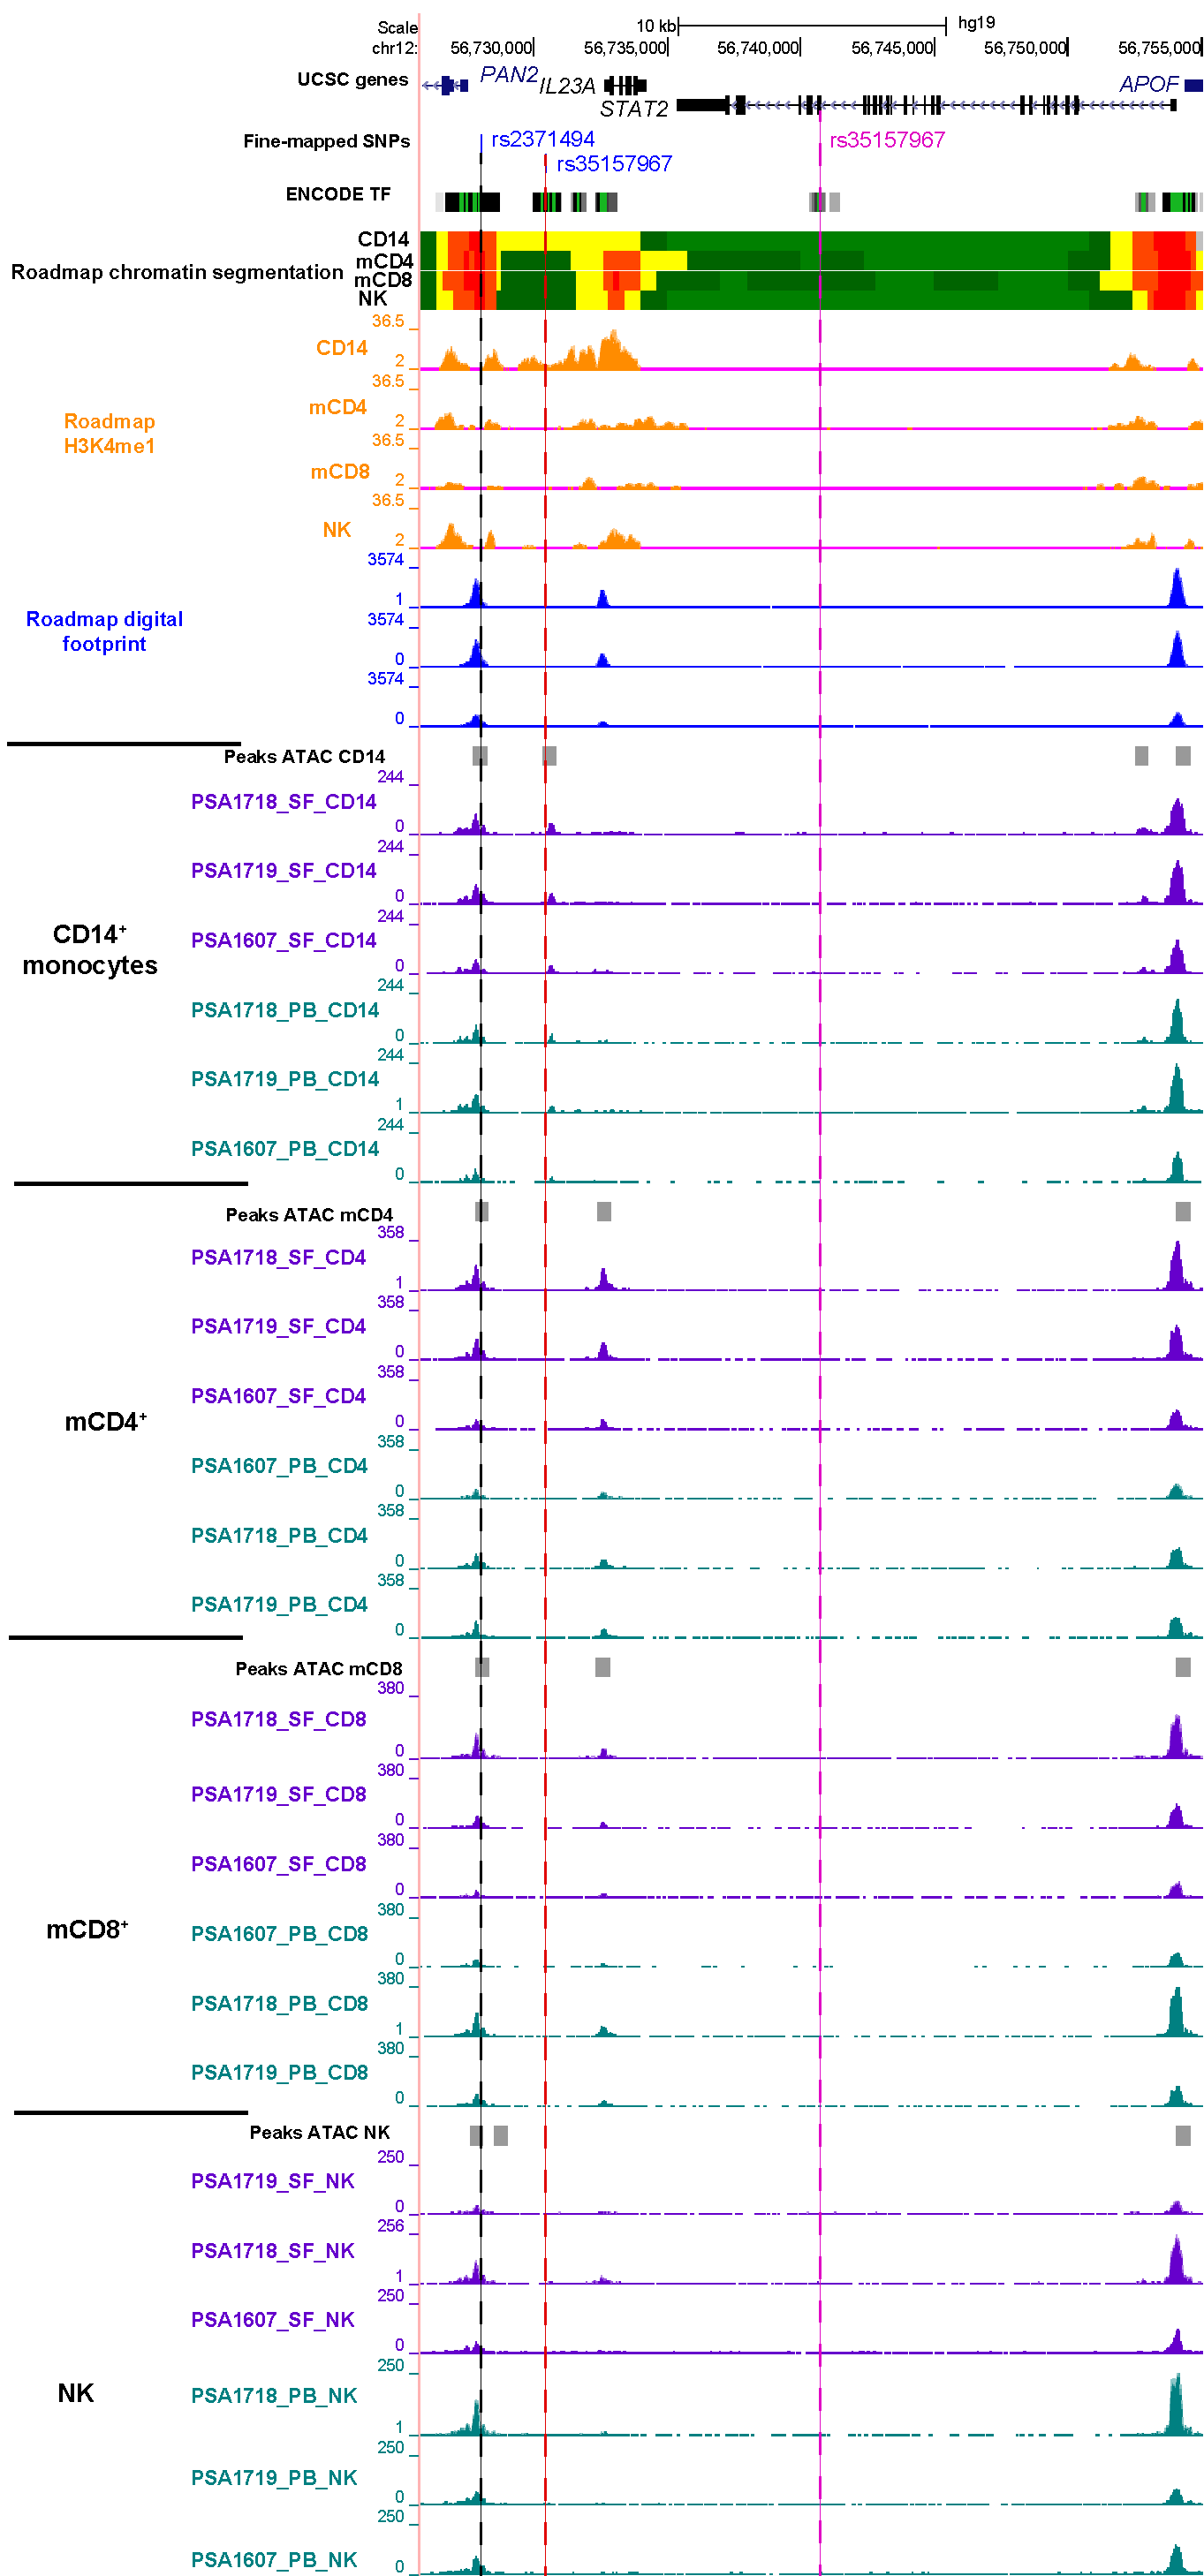
\includegraphics[width=0.6\textwidth]{./Results3/pdfs/UCSC_STAT2_IL23A_credible_set_all_cell_types_all_epigenetic_marks}
%\caption[Epigenetic landscape at the genomic location of three fine-mapped SNPs from the \textit{STAT2/IL23A} PsA GWAS signal.]{\textbf{Epigenetic landscape at the genomic location of three fine-mapped SNPs from the \textit{STAT2/IL23A} PsA GWAS signal.} UCSC visulisation of the epigenetic landscape for three relevant fine-mapped SNPs at the \textit{STAT2/IL23A} locus (x-axis), including rs2371494 (black line), rs35157967 (red line) and the missense putative damaging mutation reported by Tsoi \textit{et al.}, 2012 rs2066807 (purple line). ATAC tracks from three PsA patients and four cell types isolated from SF (purple) and PB (turquoise) are included. Publicly available epigenetic data (H3Kme1, chromatin segmentation maps, digital footprint and ENCODE cluster for TF binding) generated in the same cell types as the in-house ATAC are also included. H3K4me1 relative fold-enrichment signal and ATAC normalised counts within each cell type are shown (y-axis).}
%\label{figure:STAT2_fine_mapping_SNPs_epigenetic_track}
%\end{figure}

 

%%%%%%%%%%%%%%%%%%%%%%%%%%%%%%%%%%%%%%%%%%%%%%%%%%
\section{Discussion}


\subsection{Characterising chromatin accessibility in PsA samples}
Technological advances has enabled characterization of the epigenetic landscape in immune cells isolated from PB and SF in PsA patients. The cell types included in this study (CD14$^+$ monocytes, mCD4$^+$, mCD8$^+$ and NK) represent key players in the innate and adaptive immune response dysregulated in PsA pathophysiology. In particular, expansion of mCD4$^+$ and mCD8$^+$ cells in the synovium of PsA patients has been described, and GWAS have highlighted significant association with MHC-I and other pivotal genes involved in T cell immune response. \parencite{Taams2018}.

In this chapter I have used ATAC to identify genome-wide differences between PB and SF in four disease-relevant cell types from PsA patients. CD14$^+$ monocytes demonstrated the largest number of DARs between SF and PB (23.3\% of the investigated regions). For all the cell types, the majority of the DARs were located at intergenic and intronic regions annotated as enhancers (weak or strong), and were also enriched for eRNAs identified in each cell type by the FANTOM project \parencite{FANTOM2014}. Altogether these findings may suggest a role for the differential regions in long-range regulation of gene expression \parencite{Qu2015}. Pathway enrichment analysis of the genes proximal to the DARs revealed both commonalities and differences across cell types. In SF, enrichment for genes in the NF-$\kappa$B pathway was found in CD14$^+$ monocytes, consistent with the TNF-$\alpha$ signature and the efficacy of anti-TNF therapies already reported for PsA \parencite{Ahil2016}. Interestingly, in mCD8$^+$ T cells enrichment of DARs open in PB was found proximal to genes in the Wnt signaling pathway, such as \textit{SMAD3}. Wnt signalling is involved in many biological processes and its dysregulation is associated with a number of autoimmune diseases, such as RA \parencite{Miao2013}. In this data, the significantly increased chromatin accessibility near Wnt signalling genes in PB mCD8$^+$ cells may be related to an increased recall proliferation capacity of the circulating cells compared to the tissue-resident \parencite{Boudousquie2014}. In NK cells, increased accessibility proximal to gene members of the NK-mediated cytotoxicity pathway was found in PB compared to SF cells. NK CD56$^{bright}$ cells resident at sites of inflammation are more specialised for cytokine production than cytotoxicity \parencite{Michel2016}.  Notably, matched mass cytometry data in these patients have shown a reduced proportion of CD56$^{bright}$ cells in PB compared to SF which would be consistent with the NK-mediated cytotoxicity enrichment. 

Overall, this approach has identified robust differences in chromatin accessibility between SF and PB in relevant immune cells isolated from PsA patients. This is in line with other studies that have revealed changes in chromatin accessibility between patients and healthy controls and also across different tissues involved in disease \parencite{Scharer2016,Wang2018,Corces2016}. Although these findings suggest meaningful functional differences in chromatin accessibility between circulating and affected tissue cell populations, a limitation of pathway analysis in ATAC is linking putative regulatory regions to genes. Annotation of ATAC peaks with genes in proximity has been widely used in the literature \parencite{Scharer2016,Ackermann2016, Corces2016, Wang2018}. However, this approach fails to evaluate long range interactions, assuming accessible chromatin regulates neighbouring regions. Moreover, accessible chromatin is not a definitive marker for regulatory regions and mapping of histone marks such as H3K4me1 and H3K27ac together with eRNA quantification will help to refine the functional relevance of the identified DARs.   
   

%\subsection{Biological insights in the integration of chromatin accessibility, gene expression and proteomics data in PsA}

\subsection{Bulk gene expression profiling and integration with chromatin accessibility data}

In contrast to chromatin accessibility profiling, recent research has investigated differences in the transcriptional profile between PBMCs, bulk T cells, SFMCs and synovial tissue from PsA patients \parencite{Dolcino2015, Fiocco2015}. However, comparative analysis in matched discrete cell subpopulations from SF and PB from the same patient have yet to be reported. 

In this chapter, I have presented a pilot study characterising expression of relevant immune genes in CD14$^+$ monocytes, mCD4$^+$ and mCD8$^+$ cells isolated from SF and PB and integrated this with paired chromatin accessibility data from the same samples. CD14$^+$ monocytes and mCD8$^+$ presented the largest number of consistently modulated genes between SF and PB in this pilot analysis. The most significantly dysregulated genes between SF and PB in the four cell types were \textit{SPP1} and \textit{FN1}, the same as reported by Dolcino \textit{et al.}.  Other highly DEGs in Dolcino \textit{et al.}’s study, including \textit{TNFA}, \textit{CXCL13} or \textit{CCL18}, were also found to be modulated between SF and PB in at least one of the cell types in this pilot data. Consistent with their role in Th17 cell biology, \textit{CXCL13} and \textit{IL26} appeared significantly up-regulated in SF mCD4$^+$ and/or mCD8$^+$ cells but not in CD14$^+$ monocytes \parencite{Takagi2008}. 

The subsequent integration of transcriptome profiling with paired-ATAC data in CD14$^+$ monocytes, mCD4$^+$ and mCD8$^+$ revealed that genes with differentially modulated expression in SF and PB corresponded with nearby DARs showing changes in the same direction. Some of those DARs had also been identified as eRNAs in CD14$^+$ monocytes (e.g \textit{NFKB1}) and mCD4$^+$ cells (e.g \textit{CCR6}) by the FANTOM project. Although the characterization of those DARs as eRNAs evidences the downstream role of those regions in active transcriptional regulation, it does not unequivocally link this regulatory role to the proximal gene found to be differentially expressed between tissues by qPCR. 


The integration of differences in PB gene expression between PsA patients and controls with the cross-tissue comparison within patients led to identification of systemic, tissue-specific and putative-disease specific modulated genes in this pilot data. According to my data,  more profound transcriptional changes across PsA tissues (tissue-specific genes) were identified when compared to changes in expression between PsA patients and controls in PB for CD14$^+$ monocytes and mCD8$^+$ cells. Systemic genes for mCD8$^+$ cells included for example \textit{CCR10}, a chemokine receptor co-expressed by a subset of memory cells that preferentially migrate to skin, which has also been identified as an up-regulated gene in tCD8$^+$ cells in the psoriasis cohort (Chapter \ref{ch:Results2} and in patients with atopic dermatitis \parencite{Hijnen2005}. Interestingly, \textit{SPP1} and \textit{FN1} appeared in the tissue-specific category in the three cell types. Dolcino and colleagues had reported these genes as the two most dysregulated when comparing bulk synovial membrane transcriptome from PsA patients and healthy individuals \parencite{Dolcino2015}. My data suggests that CD14$^+$ monocytes, mCD4$^+$ and mCD8$^+$ cells may all contribute to the up-regulation of \textit{SPP1} and \textit{FN1} in the PsA synovium membranes. The \textit{SPP1} protein product, osteopontin, is a cytokine and chemokine expressed by many cell types, including monocytes/macrophages and T cells. It is involved in cell migration, adhesion and cell-mediated immune response through regulation of T cells, importantly in Th-17 \parencite{Morimoto2010}. \textit{SPP1} also plays a role in other chronic inflammatory and autoimmune diseases \parencite{Rittling2015}. \textit{FN1} encodes fibronectin-1, a main component of the cartilage matrix, involved in cell adhesion, migration, growth and differentiation and found to be highly expressed in RA inflamed synovium \parencite{Chang2005}.  Moreover, \textit{FN1} has been shown to induce bone resorption mediated by pro-inflammatory mediators, such as nitric oxyde and IL-1$\beta$ \parencite{Gramoun2010}.  In Dolcino’s data \textit{FN1} up-regulation was only found when comparing synovial membranes of PsA versus controls, and no changes were reported in PB samples, altogether suggesting the tissue-specificity of this dysregulation in PsA. Furthermore, the identification of DARs open in SF at the promoter and 3’ downstream of \textit{FN1} in CD14$^+$ monocytes may suggest a link between changes in modulation of gene expression and chromatin accessibility in this particular cell type. 

In contrast to the observation in my pilot study, Dolcino also showed moderate up-regulation of \textit{SPP1} expression in PB from PsA patients compared to controls. This could be explained by the fact that Dolcino's study was performed in bulk PBMCs and dysregulation of \textit{SPP1} in CD14$^+$ monocytes, mCD4$^+$ and mCD8$^+$ cells may be tissue-specific. However, this could also be the result of the small number of qPCR replicates and \textit{SPP1} dysregulation in PB between PsA and healthy samples failing to reach significance in my study. Overall, up-regulation of these two genes in SF cells reflect the activation of chemotaxis and  infiltration of circulating monocytes and T cells,  activation of the Th-17 immune response and dysregulation of osteoclast bone remodeling , all of which are pivotal in PsA pathophysiology, particularly at the inflamed tissue \parencite{Durham2015, Mensah2017}.

An example of an interesting putatively disease-specific gene identified by this study was \textit{GPR68}, up-regulated in mCD4$^+$ PsA PB compared to controls with expression further increased in SF. \textit{GPR68} is a G protein-coupled receptor (GPCR), expressed in T cells and others, that undergoes activation through pH acidification, characteristic of synovial tissues under inflammation \parencite{Biniecka2016, Saxena2011}. Interestingly, \textit{GPR65}, another member of the acid-sensing GPCR family, has been associated with a number of immune mediated diseases, including AS, CD and MS \parencite{Cortes2013,Lassen2016,Wirasinha2018}. GPR65 was found to be a marker of pathogenic Th17 cells in the murine and human systems \parencite{Gaublomme2015, Al-Mossawi 2017}. Unfortunately, GPR65 was not included in the gene array used in this study. Indeed, the use of a gene array rather than a transcriptomics approach using RNA sequencing is a limitation of this study. 

In terms of relevant biological processes, pathway analysis using consistently modulated genes between SF and PB in this data revealed enrichment for TLR and NOD-like signalling pathways in CD14$^+$ monocytes. This was consistent with the relevance of TLR and NOD-like receptors for rheumatic diseases \parencite{McCormack2009}. Up-regulated expression of \textit{TLR1} and \textit{TLR2} was significant in SF CD14$^+$ monocytes compared to PB and a similar trend in \textit{TLR4} expression was also observed but failed to reach significance in this pilot study.  These finding were in line with some studies that have identified increased \textit{TLR-2} and \textit{TLR-4} expression in SFMCs compared to PBMCs in patients with juvenile idiopathic arthritis \parencite{Myles2011}. The relevance of NOD-like signaling has also been highlighted in the genome-wide trancriptomic analysis in lesional and uninvolved psoriatic skin presented in Chapter \ref{ch:Results2}, reinforcing the role of NOD-like signalling in the inflammatory response at the site of inflammation. The cross-talk between the TLR and NOD-like signalling pathways was further evidenced by network-based analysis in this data highlighting increased activation of the NF$\kappa$B TF in SF, particularly in CD14$^+$ monocytes. In my data, enrichment of DARs open in SF in the proximity of genes within the NF-$\kappa$B pathway was also found and further supported transcriptionally by the consistent up-regulation of downstream genes such as \textit{TNFA}, textit{CCL2} and \textit{CCL5} in SF CD14$^+$ monocytes. Moreover, analysis for conserved TFBS motifs in the ATAC data revealed enrichment for NF-$\kappa$B binding motifs within DARs open in SF CD14$^+$ monocytes but not in DARs open in PB (data not shown).

The enrichment of differentially modulated genes between SF and PB in mCD4$^+$ for the IL-10 signalling pathway was particularly interesting in the context of flow cytometry from the same three patients evealing expansion of Tregs in SF compared to PB (data not shown). Tregs are characterised by the expression of anti-inflammatory cytokines, including IL-10 \parencite{O’Garra2004}. The qPCR transcriptomic data showed in SF mCD4$^+$ and mCD8$^+$ a significant increase in expression of the IL-10 receptor subunit $\alpha$ \textit{IL10RA} and a similar trend for \textit{IL10} up-regulation (pval=0.14 and 0.07, respectively) compared to PB. Altogether, this could suggest that inflammation in PsA is refractory to the immunomodulatory effects for IL-10 signalling in SF o counterbalanced by the immunostimulatory properties of this cytokine, which could be one of the reason for failure of IL-10 agonist therapy in CD and psoriasis \parencite{Marlow2013, Kimball2002}. 

%Overall, this work sought to characterise gene expression and chromatin accessibility differences between SF and PB, and has revealed interesting observations across all cell types. 
\subsection{The relevance of monocytes and investigation of other cell types}
In this exploratory data, CD14$^+$ monocytes showed the most DARs and confidently modulated genes between SF and PB as well as functionally relevant pathway enrichment. The work presented is part of a collaborative multi-omics PsA pilot study. In light of this thesis, and for the cohort size available at the time of analysis, CD14$^+$ monocytes were chosen as the cell type to further explore by scRNA-seq and integrate with mass cytometry data. mCD4$^+$ and mCD8$^+$ also showed relevant changes in chromatin accessibility and gene expression, and have been identified as the two cell types undergoing greater expansion in the synovium of PsA patients. Colleagues involved in this project have since performed differential TCR clonality analysis between SF and PB using PsA samples included in this thesis. Interestingly, a significant number of mCD8$^+$ TCR clones with potentially shared antigen recognition across patients were found to be enriched in SF compared to PB (manuscript in preparation).  

\subsection{Characterisation of monocytes by scRNA-seq}
Monocytes are very plastic cell populations that undergo cell differentiation at the site of inflammation, with differences that may be better captured at the single-cell level. In this pilot experiment, cluster identification in scRNA-seq from combined SF and PB monocytes using a conservative approach (see \ref{Discussion_scRNAseq}) revealed two main subpopulations (CC-mixed and CC-IL7R). CC-mixed appeared as a large heterogenous cluster in contrast to the CC-IL7R subpopulation, characterised by cells consistently expressing \textit{IL7R}, \textit{IL32} and textit{CCL5}, amongst other markers. According to the scRNA-seq data, the CC-IL7R cluster represented around 3\% of the total monocytes and had approximately the same number of cells from SF and PB (3 and 2.7\%, respectively). Conversely, flow cytometry data in PsA and AS patients have shown up to 35\% of the total SF CD14$^+$ monocyte to be IL-7R$^+$ versus approximately 1\% in PB (in revision \parencite{Al-Mossawi2018}). This could be due to discrepancies between gene expression and protein translation acknowledged in the literature but may also be a consequence of lower sensitivity of scRNA-seq in quantifying gene expression \parencite{Liu2016,Islam2014}. This may be leading to underestimate the CC-IL7R cluster size and the predominance of SF monocytes IL-7R$^+$ in the contribution towards this cluster. Differences in sensitivity between qPCR and scRNA-seq may also partly explain the limited overlap of differentially expressed genes between SF and PB when using qPCR and scRNA-seq. Although the same top dysregulated genes (including \textit{SPP1}, \textit{FN1} or \textit{OLR1}) were identified by both techniques, a modest number of significantly modulated genes found by qPCR were reproduced by the scRNA-seq analysis in the CC-mixed cluster. In terms of chromatin accessibility, the comparison of FCs from contrasting SF and PB chromatin accessibility in CD14$^+$ monocytes and scRNA-seq expression in the CC-mixed cluster only showed moderate correlation. This limited correspondence between chromatin accessibility and gene expression has also been reported by other studies and may be also the result of aforementioned limitations in annotating accessible chromatin with a putative target gene \parencite{Ackermann2016,Wang2018}.

The identification of sub-populations of monocytes expressing IL-7R$^+$ is of biological interest as \textit{IL7R} polymorphisms are associated with a number of chronic inflammatory diseases, including AS and MS \parencite{Gregory2007, Cortes2007}. Although the role of IL-7 and IL-7R in mediating the immune response was only characterised in T cells, the relevance of IL-7R in CD14$^+$ monocytes under LPS stimulation has been demonstrated in eQTL studies and also at the protein level in a manuscript under review, to which I have contributed \parencite{Fairfax2014, Al-Mossawi2018}. Al-Mossawi and colleagues identified a distinct transcriptional profile of the IL7R cluster in PsA SF monocytes very similar to the gene expression profile from IL7R$^+$ \textit{in vitro} stimulated monocytes. Interestingly the \textit{IL-7R} locus showed differentially accessible chromatin in PsA SF and was one of the top DEGs in the CD14$^+$ monocyte qPCR array. Moreover, my analysis \textit{CD44} appeared to be up-regulated in SF compared to PB in the CC-IL7R cluster. Interestingly, \textit{CD44} is the receptor for osteopontin and this observation may suggest that the SF CC-IL7R cells may be more responsive to this cytokine. Taken together, this data supports a role for IL-7 signalling in PsA circulating and tissue monocytes in chronic inflammation.

Pathway enrichment analysis using scRNA-seq DEGs between SF and PB in the CC-mixed cluster identified biologically relevant processes, including MHC-II Ag processing, IFN signaling and extracellular-matrix components, amongst others. Interestingly, up-regulation of \textit{IFI6} and \textit{IFITM3}, two of the genes contributing to the enrichment of this pathway, have also been identified as markers of a subpopulation of IFN-$\gamma$ activated monocytes in from RA synovial tissue using scRNA-seq \parencite{Zhang2018}. In addition to the IFN-$\gamma$ activated, this study identified other three cluster within RA and osteoarthritis (OA) patients monocytes; however IL-7R$^+$ were not explicitly mentioned. Genes enriched for the extracellular-matrix pathway included members of the S100 protein family, previously reported to be dysregulated in lesional skin from psoriasis patients (Chapter \ref{ch:Results2}), which are also involved in joint erosion and development of arthritis \parencite{Raghunatha2012}. Two genes of this family, \textit{S100A8} and \textit{S100A9}, were up-regulated in lesional skin compared to uninvolved, but down-regulated in SF CC-mixed monocytes in this data.  The lack of overlap between the pathways identified for the DEGs in the CC-mixed and those found by qPCR in bulk CD14$^+$ monocytes could be due the result of the qPCR array being biased to a small number of genes versus the unbiased approach of the scRNA-seq.

\subsection{Mass cytometry in CD14$^+$ monocytes and the integration with chromatin accessibility and transcriptomic data}
Single-cell mass cytometry in matched PB and SF was first conducted in the same three PsA with available paired ATAC and/or qPCR data. Despite technical limitations, mass cytometry in this samples identified a greater percentage of CD14$^+$ monocytes producing TNF-$\alpha$ in the SF compared to PB, in lines with the chromatin accessibility and transcriptomic data suggesting increased NF-$\kappa$B activation in this tissue. A cohort with additional ten SF and PB PsA samples validated with statistical significance the TNF-$\alpha$ observation. Moreover, the expanded cohort also demonstrated increased percentage of CD14$^+$ monocytes actively producing MCP-1 and osteopontin in SF compared to PB, consistently with the up-regulation in \textit{CCL2} and \textit{SPP1} expression in SF. A study using quantitative mass cytometry comparing SF from PsA and OA as control did not identify any of these three proteins to be up-regulated \parencite{Cretu2014}. Conversely, another study using enzyme-linked immunosorbent assay (ELISA) reported an increased production of TNF-$\alpha$, amongst other cytokines, in PsA SF compared to OA \parencite{Partsch1997}. 

Notably, \textit{CCL2}/MCP-1 represented a good example of correlating differences between SF and PB monocytes across chromatin accessibility, gene expression and protein production data. Dolcino’s study did not identify up-regulation of \textit{CCL2} expression in PsA synovial membranes when compared to controls, which could be due to these differences being masked by the mix of cell populations in this tissue. Interestingly, increased levels of MCP-1 in SF, similarly to the observation made by our collaborators in Basle, were previously reported, and correlation with the infiltrated levels of T cells was also demonstrated \parencite{Ross2000}. Regarding the open DAR in SF proximal to \textit{CCL2}, no eQTL or chromatin conformation data in CD14$^+$ monocytes has revealed direct evidence for a relationship between differential expression of \textit{CCL2} and changes in chromatin accessibility in this nearby region. 

\subsection{Challenges and future perspectives in multi-omic approaches}
\label{Discussion_scRNAseq}

The work presented in this chapter is an exploratory study and a proof of principle for the implementation of a multi-omics approach, which represents a very powerful strategy to dissect disease pathophysiology in a cell type specific manner. Nevertheless, a number of limitations and challenges were encountered and need to be taken into account to contextualise these results. One limitation is the small sample size (n=3) and the lack of paired data across all the techniques presented. This results from difficulties of recruiting PsA patients na\'{i}ve for any treatment, the logistical difficulties to coordinate all of the techniques from the same sample, and the high cost of this approach. A further limitation in this study is the lack of PB from healthy controls or SF from another autoimmune or non-inflammatory joint disease, as included by other studies \parencite{Fumitaka2018, Dolcino2015,Zhang2018}.  The definition and categorisation of the qPCR significantly modulated genes into systemic, tissue-specific and putative disease-specific was particularly limited by a lack of control samples to compare to the SF cells and the use of a biased transcriptomic analysis using a qPCR array.
Another challenge in this study relates to the analysis and integration of scRNA-seq and mass cytometry data. Both techniques still represent emerging fields were no consensus has been reached on the best strategy to combine samples across patients and experiments, accounting for batch effect. In this exploratory study, monocytes were identified from each SFMCs and PBMCs scRNA-seq sample and combined using CCA for further subpopulation identification. However standard resolution for cluster identification yielded potentially spurious subpopulations, leading to the adoption of a more conservative approach to define clusters in this particular analysis. This may be the consequence of remaining batch effects, and alternative methods of combining samples from the different experiments should be investigated. In this respect, the identification of robust and stable subpopulations through cluster analysis will benefit from the implementation of algorithms designed for cluster validation such as Silhouettes, which has recently been used successfully in the field of single-cell \parencite{Rousseeuw1987, Zhang2018}. In addition to this, incorporation of bulk RNA-seq data from CD14$^+$ monocytes will help interpretation and validation of the scRNA-seq results. In mass cytometry, to reduce batch effects patient samples are undergoing \textit{ex-vivo} fixation and cryopreservation followed by simultaneous staining and barcoding. Moreover, different methodologies for cluster identification and annotation are also being explored and so far no clear clusters have confidently been found.

In terms of data integration, this pilot study used relatively simplistic multi-omics data integration limited by sample size, technical aspects and time scale, and provides a platform for future validation studies. A more systematic integrative approach should be implemented for the expanded cohort to establish appropriate correlation across datasets. Currently Zhang and colleagues have presented the most exhaustive methodology to integrate bulk-RNA-seq, scRNA-seq, mass cytometry and flow cytometry into multi-modal transcriptomic and proteomics profiles, but their work is still under peer review \parencite{Zhang2018}. This strategy has revealed disease-specific functional expanded subpopulations amongst the most relevant cell types in RA pathophysiology. Additionally, the correlation between bulk ATAC and scRNA-seq is clearly limited by the different scales of the two approaches. Therefore, generation of scATAC-seq data, identification of clusters based on chromatin profiling and appropriate methods for the overlap with scRNA-seq populations should be used to have a better understanding of the correlation between chromatin accessibility and gene expression at the single-cell level \parencite{Duren2018}.


\subsection{The use of PsA functional data to inform fine-mapping GWAS loci}
Integration of epigenetic data with fine-mapped SNPs from GWAS studies has been widely demonstrated to be a powerful tool to further narrow down candidate causal variants, particularly for intergenic or intronic signals not driven by LD with missense coding SNPs \parencite{Bunt2015,Farh2014}. Although DARs between SF and PB in four cell types did not show any overlap with SNPs from the credible set, significant enrichment of fine-mapped SNPs for accessible chromatin was demonstrated in all four cell types. A number of SNPs from the 5q31 credible set in my analysis overlap accessible chromatin and eQTL signals in the same cell type. Integration of tCD4$^+$ and tCD8$^+$ eQTL from Kasela \textit{et al.} confirmed the association between SNPs from the 5q31 GWAS signal and T cells \textit{SLC22A5} expression previously reported in a smaller study by Bowes \textit{et al.}, and also suggested a potential role for the 5q31 PsA-specific GWAS association in regulating \textit{P4HA2} and \textit{SLC22A5} expression in unstimulated and stimulated monocytes. \textit{SLC22A5} is a cell membrane transporter of carnitine involved in fatty acids metabolism and has been prioritised by an in-house pipeline as the third most promising druggable candidate for the treatment of psoriasis. Supporting evidence highlights the implications of this gene in other inflammatory conditions such as CD and the potential as a druggable therapeutic target in PsA \parencite{Leung2006}.
 
Contrary to the initial hypothesis, the integration of fine-mapping data and DARs between SF and PB in PsA relevant cell types failed to show overlap in any of the four studied cell types. %For associations driven by exonic non-synonymous missense mutations, such as \textit{TRAIF3IP2}, changes in chromatin accessibility are not necessarily expected. 
For non-coding signals hypothesised to have a regulatory role, these results may suggest that fine-mapped SNPs from PsA GWAS loci do not have a tissue specific effect in chromatin accessibility changes for any of these cell types. These results may also be biased by the small size in my differential chromatin accessibility analysis and the limited power of the fine-mapping analysis using only a subset of the PsA GWAS cohort. Studying variation in chromatin accessibility upon genotype of the fine-mapped SNPs, similar to the example of chr2p15 presented in Chapter \ref{ch:Results2}, may be more informative when integrating epigenetics at a GWAS associated locus.


\subsection{Conclusions}
The strategy and analysis presented in this chapter is a proof of principle for conducting a multi-omics approach on clinical samples in a cell type and tissue-specific manner. The study of chromatin accessibility in immune cells from SF and PB of PsA patients has demonstrated differences across the two tissues and shown specific enrichment for relevant pathophysiological functional pathways. Transcriptional analysis conducted on the same samples for a number of genes involved in the immune response has also revealed differential expression between the two tissues in all the cell type and shown some of those genes to be proximal to regions presenting changes in chromatin accessibility in the same direction. In this study, both data types highlighted CD14$^+$ monocytes as the cell type presenting the largest number of significant changes in chromatin accessibility and consistent modulation of gene expression between SF and PB, with enrichment for pathways leading to inflammation through NF-$\kappa$B activation and subsequent cytokine and chemokine production. Implementation of scRNA-seq has shown the ability of this approach to identify sub-populations within SF and PB CD14$^+$ monocytes. Lastly, relatively basic integration of mass cytometry data has confirmed increased ability of SF CD14$^+$ monocytes to produce a number of cytokines and chemokines and supported differences in chromatin accessibility and gene expression between the two tissues at the protein level. Overall, this chapter has shown that in PsA the pro-inflammatory environment at the site of inflammation drive changes in chromatin accessibility, gene expression and protein production that distinguish circulating cells from those infiltrated homing the involved tissue.




%In Dolcino PSA vs HV SF comparison also detected more up genes than down in the array analysis
%Say which cell types drive more the top changed gene
%
%
%
%%NOD-like in PsA: https://www.ncbi.nlm.nih.gov/pmc/articles/PMC4792137/
%%TLR in PsA: https://www.ncbi.nlm.nih.gov/pmc/articles/PMC2787278/
%
%% SIGRR downregulation by LPS https://www.ncbi.nlm.nih.gov/pmc/articles/PMC4140261/
%% CCL2 and CXCL10 in PsA
%
%The integration of the varied types of datasets that can be generated from clinical samples of a wide range of complex diseases remains challenging. It requires the implementation or development of new algorithms in order to integrate them into a systematic way
%Machine learning has been used for RA https://onlinelibrary.wiley.com/doi/epdf/10.1002/art.40428
%CCA analysis also for RA Zhang2018	


%Regarding the low number of qPCR DEGs between SF and PB in total CD14$^+$ monocytes reproduced by the scRNA-seq in any of the two main clusters identified could be explained by the differences in the cell sorting (FACS versus \textit{in silico} expression markers), the low number of replicates for each assay as well as different sensitivity of the two technologies.   


%IL7R 3'UTR increased chromatin accessibility
%https://journals.plos.org/plosone/article?id=10.1371/journal.pone.0040828
